\chapter{Estado de Arte Detalhado}
\label{a:ea}

\section{SurveyMonkey}
\label{surveyMonkey}

O SurveyMonkey é uma plataforma \acrfull{saas} de criação de formulários online que permite recolher e visualizar informações do público alvo através de formulários.

O SurveyMonkey é uma plataforma que dispões de diversos planos de pagamento, e por isso mesmo, apesar de estar disponível um plano gratuito, tem acesso apenas a algumas das funcionalidades e em cada formulário, no máximo, poderá ter 10 perguntas ou elementos.
É necessário criar conta para aceder às funcionalidades da plataforma, dando a opção de utilizar serviços externos para esse efeito : Facebook\cite{face}, LinkedIn, Google\cite{gaccount} e Microsoft\cite{microsoft}.
No painel principal, como podemos ver na Figura \ref{fig:survey-dashboard} temos acesso rápido aos formulários recentes e a algumas métricas sobre os mesmos. Outra forma será aceder aos formulários do utilizador através da barra de navegação. 


\begin{figure}[ht!]
	\begin{center}
		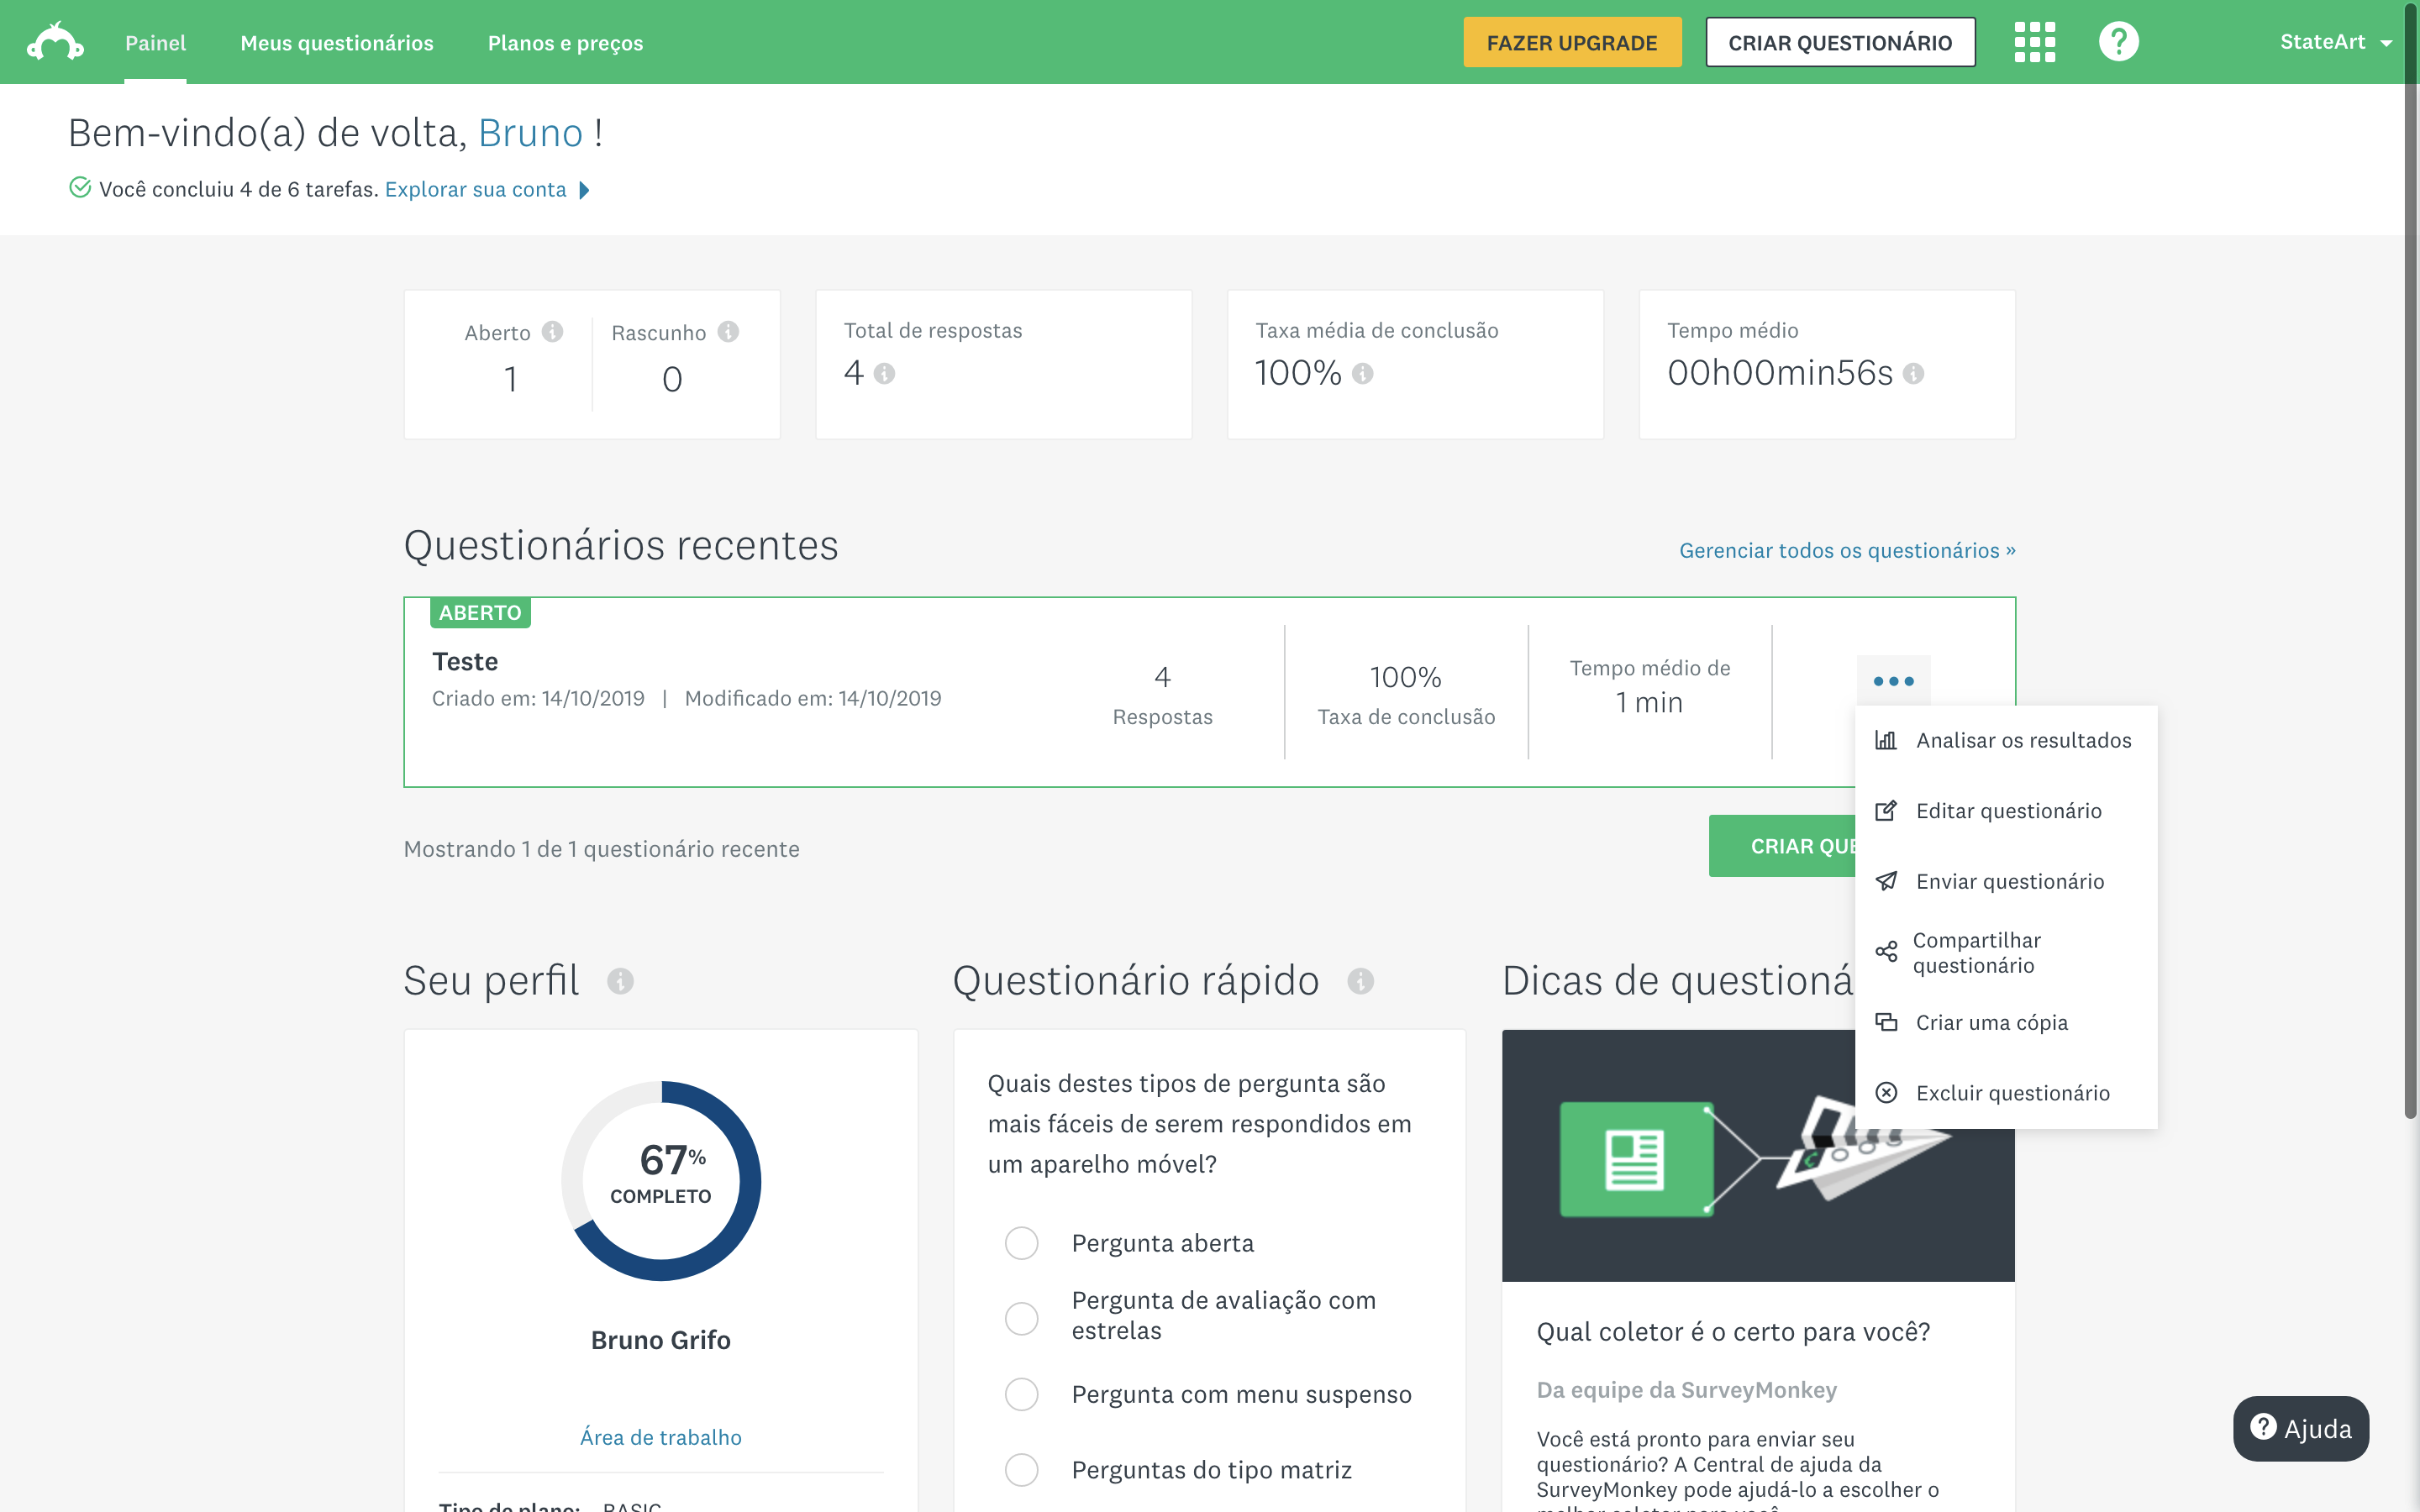
\includegraphics[width=1\textwidth]{img/sm/survey-dashboard}
		\caption{SurveyMonkey - Painel de Controle }
		\label{fig:survey-dashboard}
	\end{center}
\end{figure}

\newpage

\begin{figure}[ht!]
	\begin{center}
		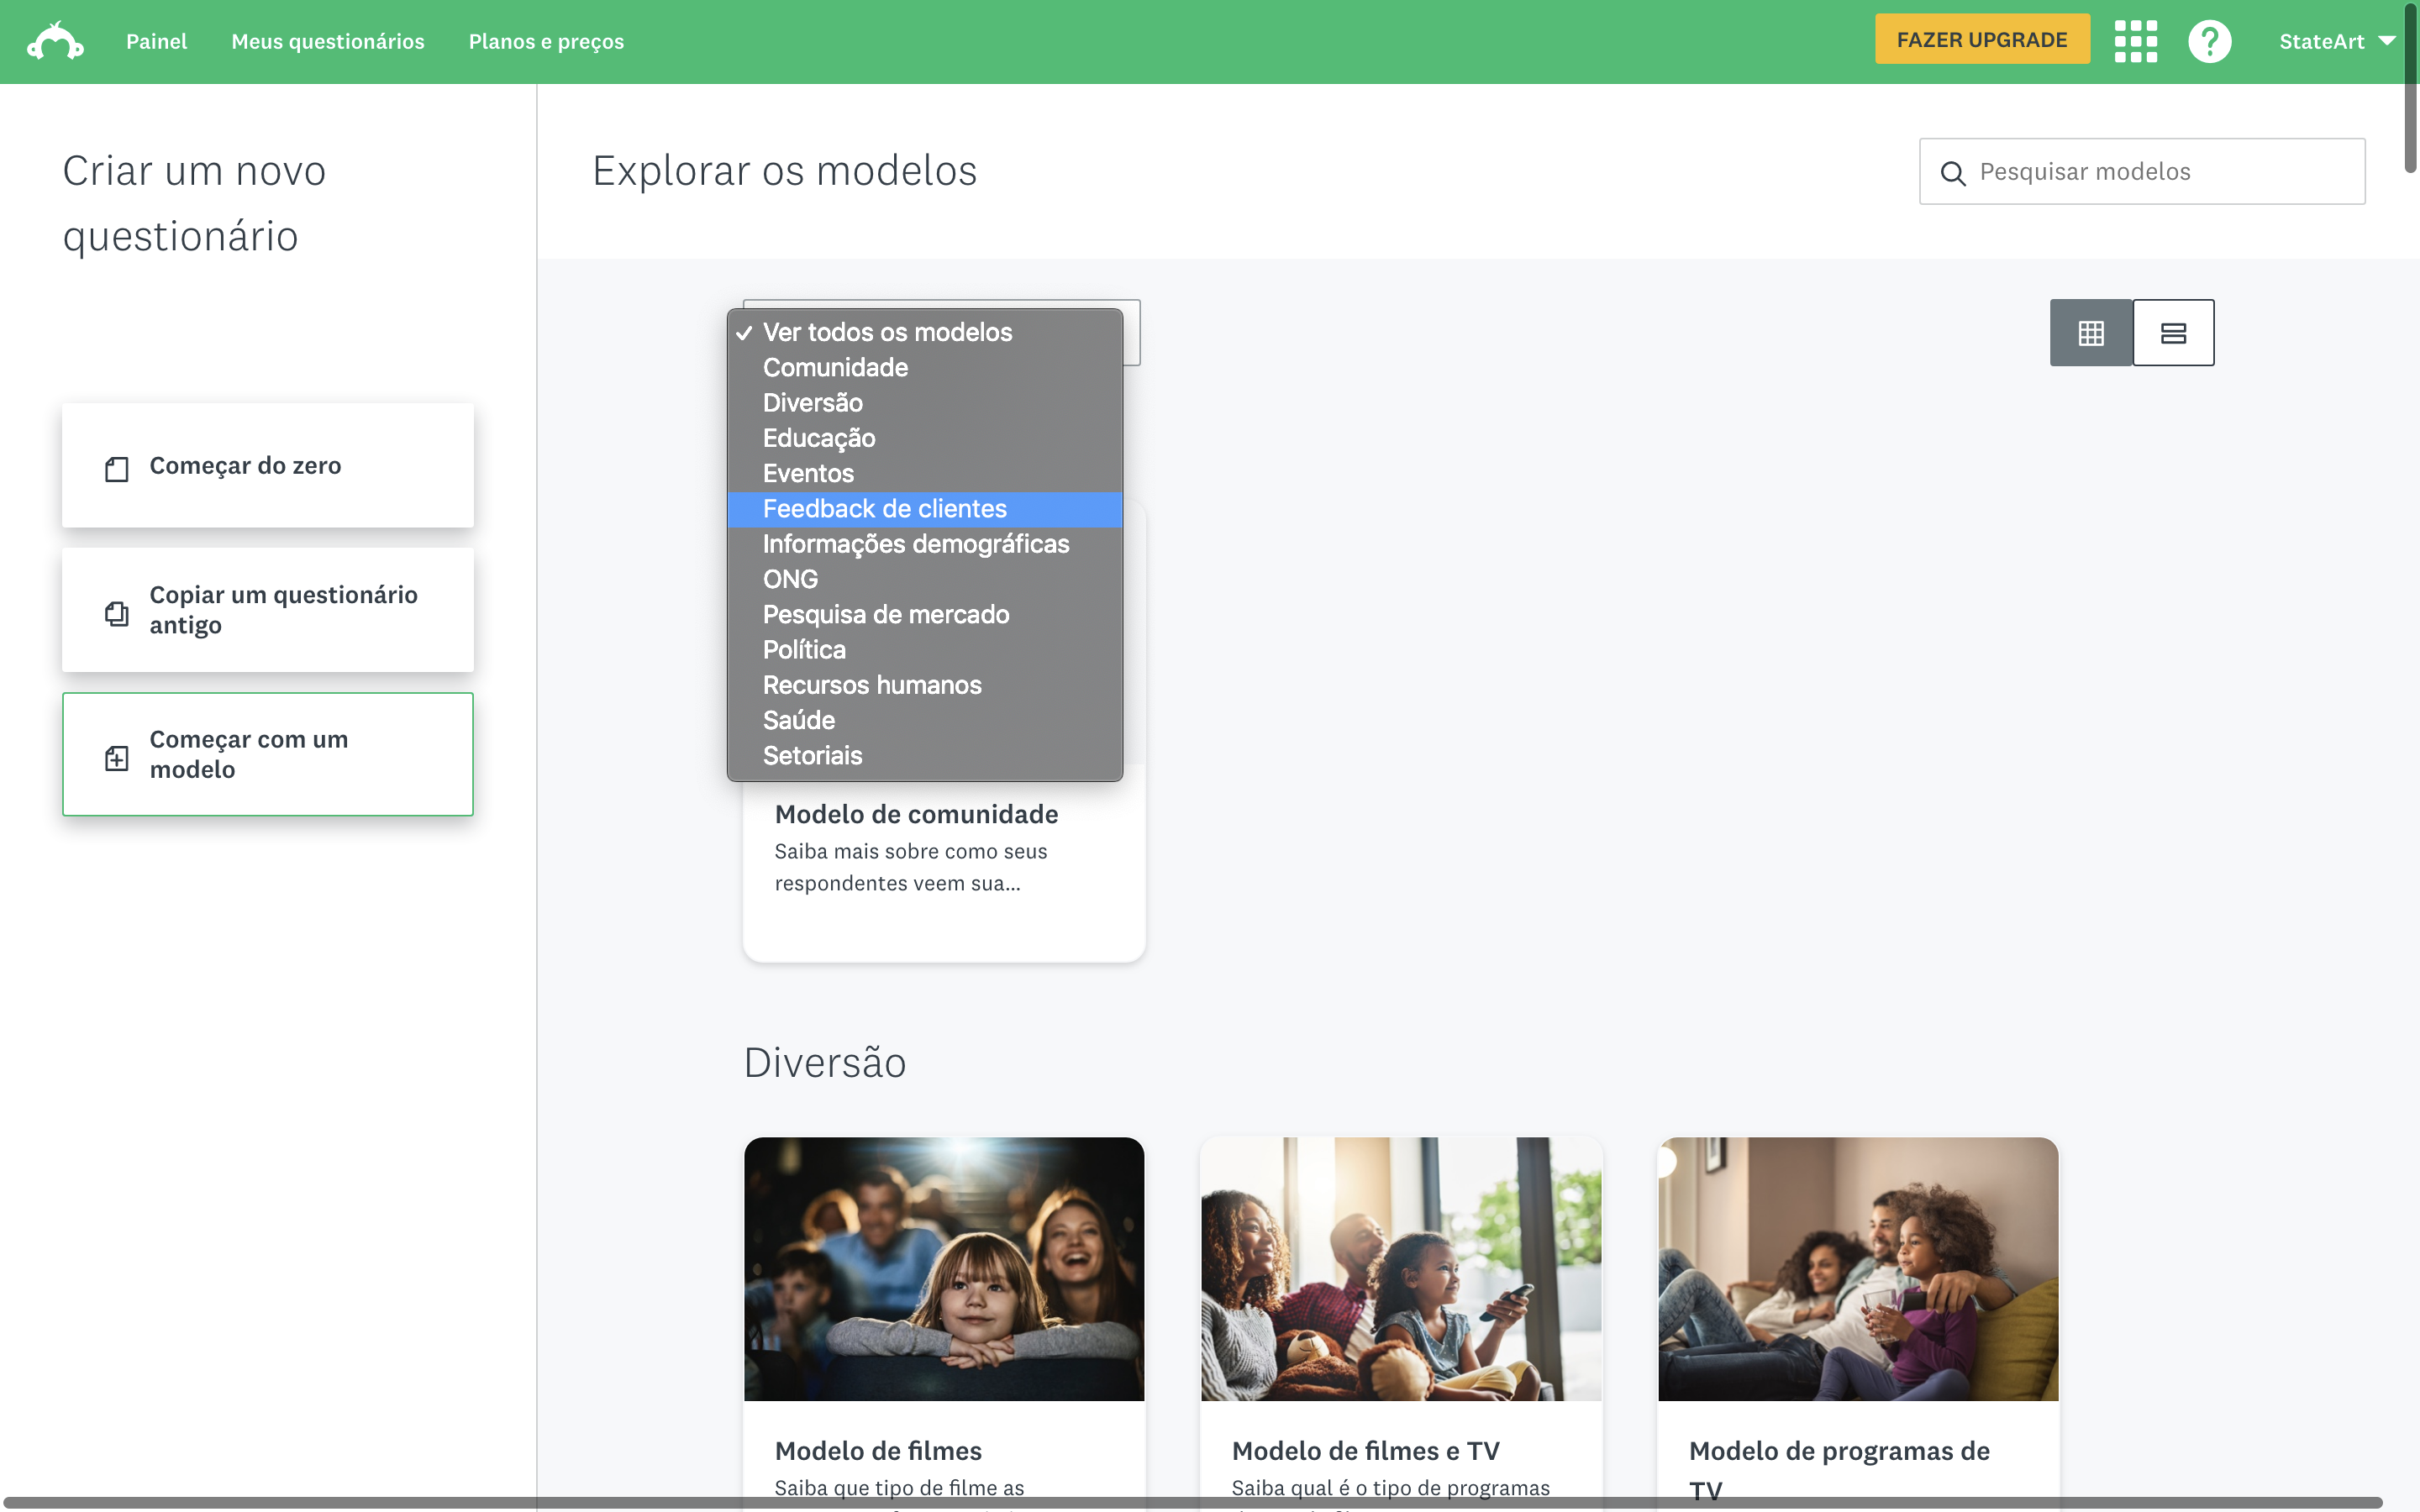
\includegraphics[width=1\textwidth]{img/sm/survey-form-create}
		\caption{SurveyMonkey - Formulários modelo }
		\label{fig:survey-form-create}
	\end{center}
\end{figure}

Quando se inicializa a criação de um novo formulário, a plataforma dá opção de começar do zero ou de utilizar um formulário modelo como podemos ver na Figura \ref{fig:survey-form-create}. Começando um formulário do zero como podemos ver na Figura \ref{fig:survey-form-banck2}, temos acesso a uma série de funcionalidades que vamos explorar e analisar em seguida.

\begin{figure}[ht!]
	\begin{center}
		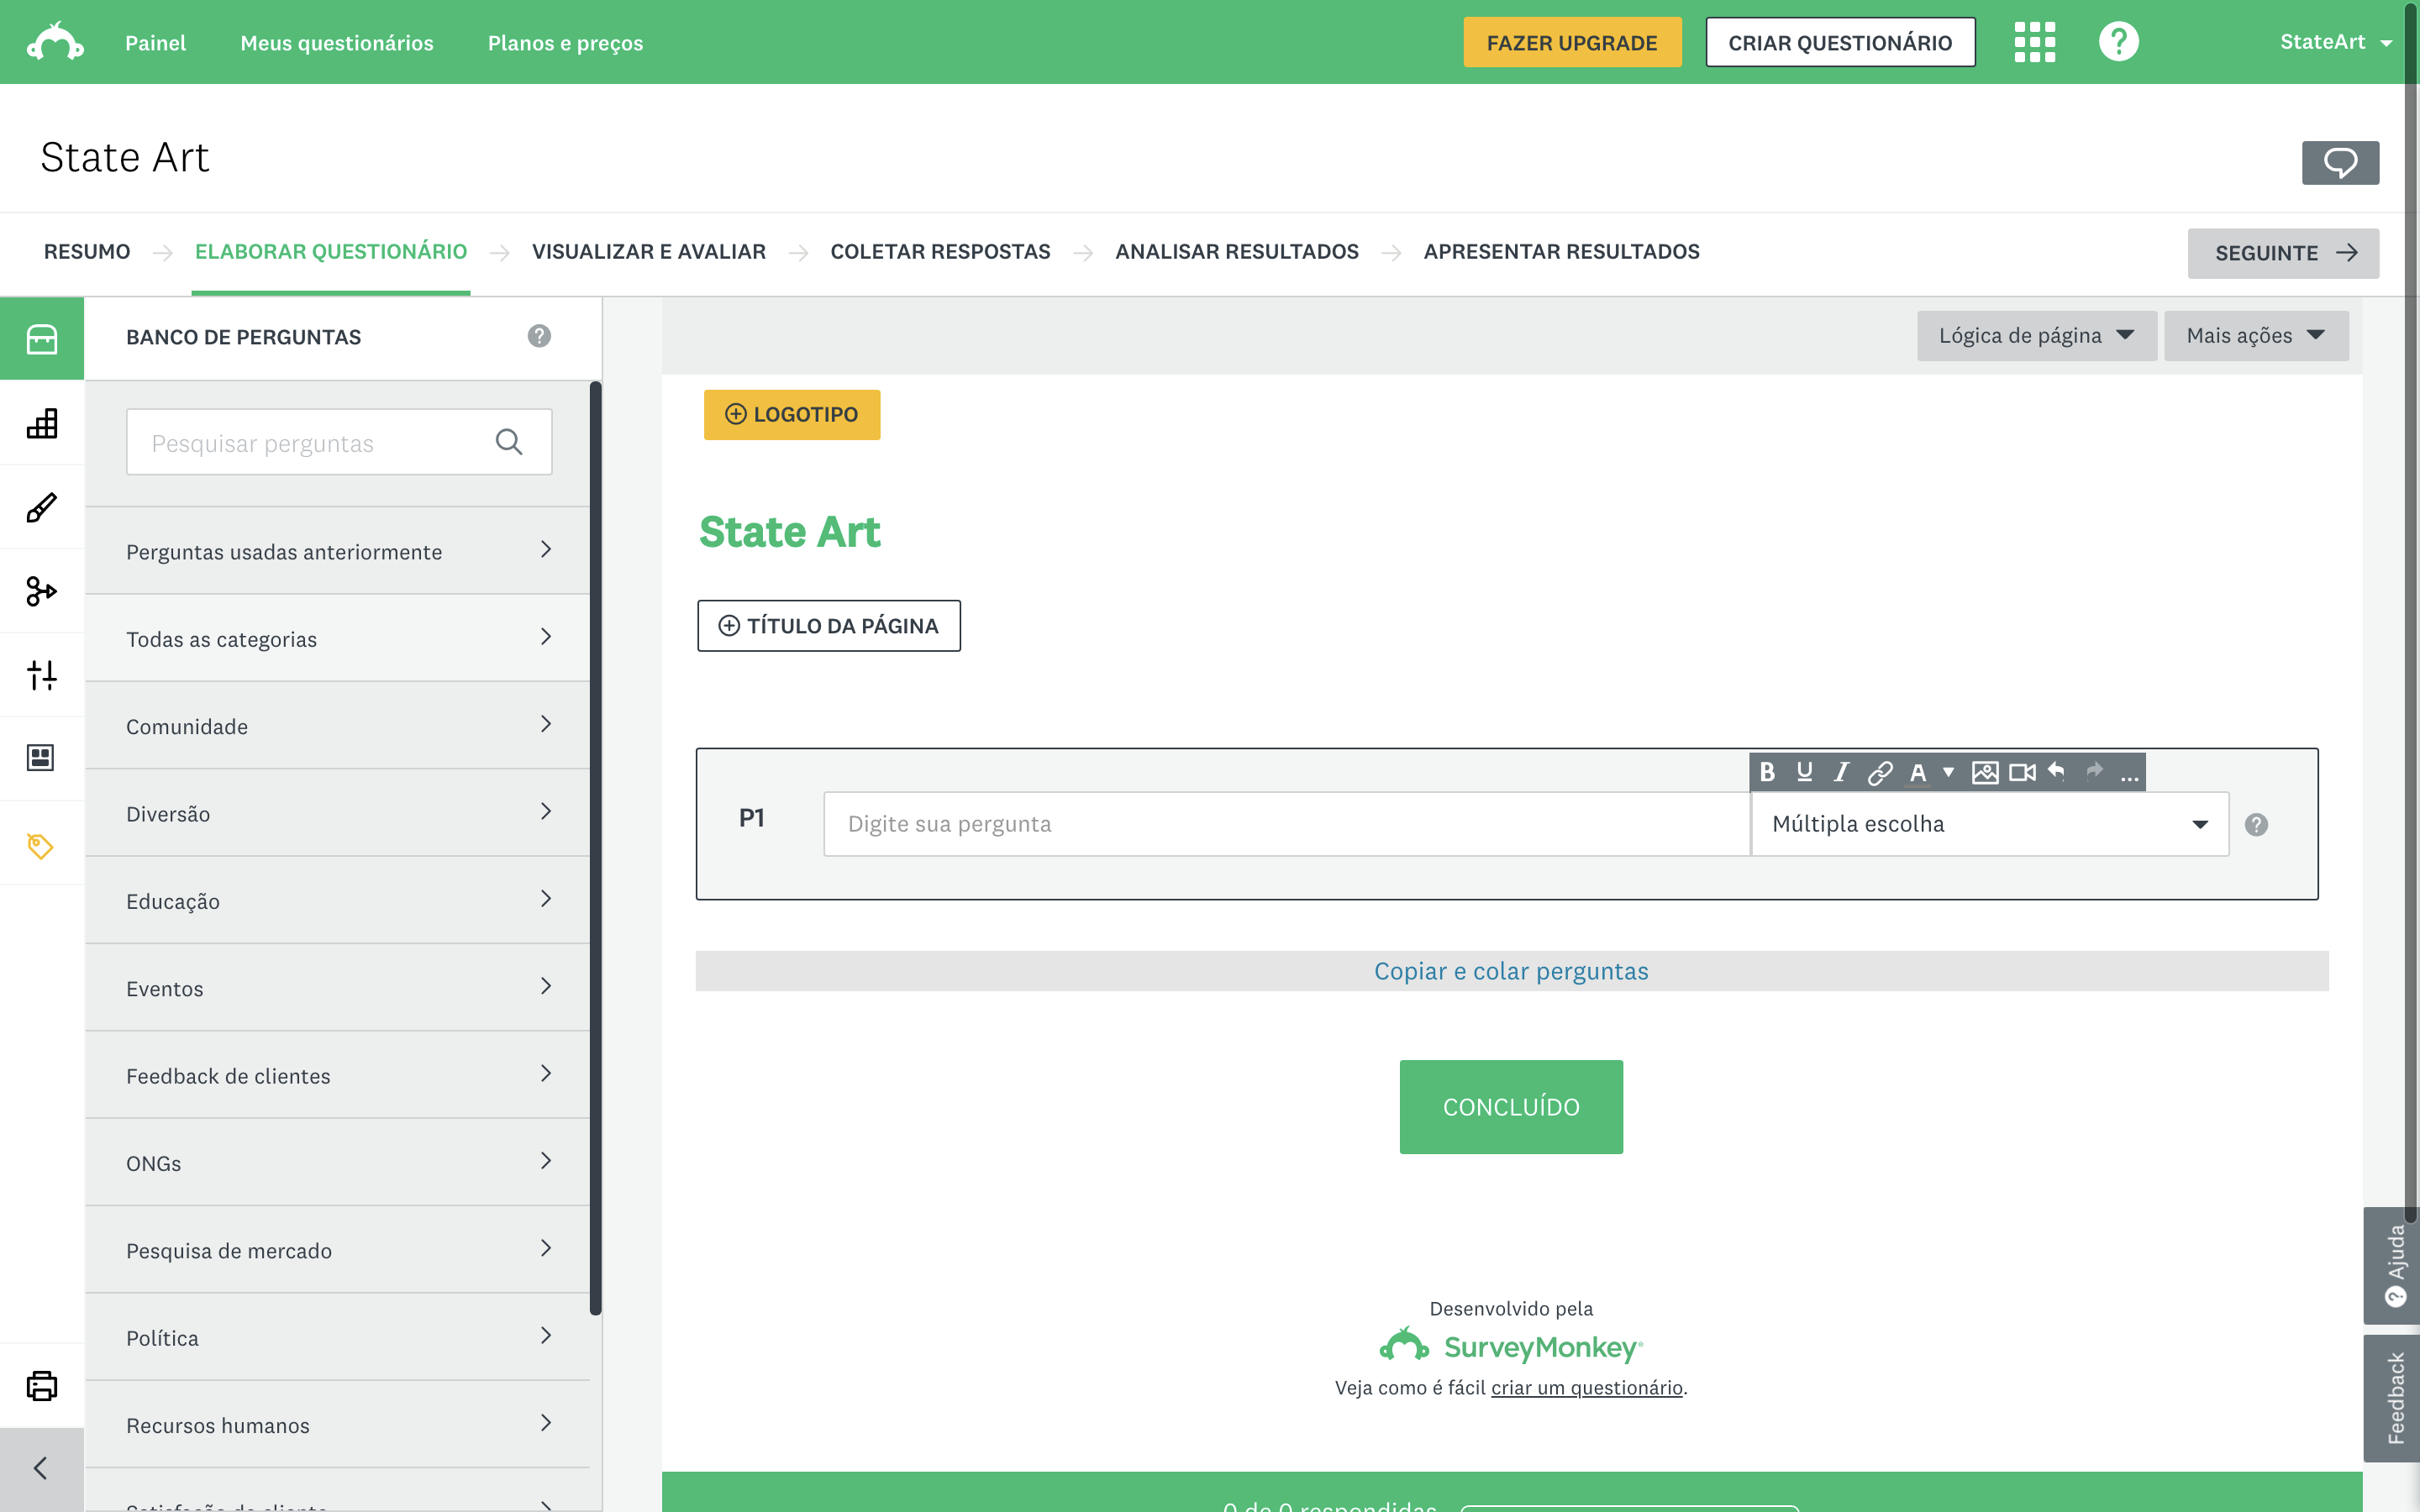
\includegraphics[width=1\textwidth]{img/sm/survey-form-bank2}
		\caption{SurveyMonkey -  Perguntas Modelo}
		\label{fig:survey-form-banck2}
	\end{center}
\end{figure}


\begin{figure}[ht!]
	\begin{center}
		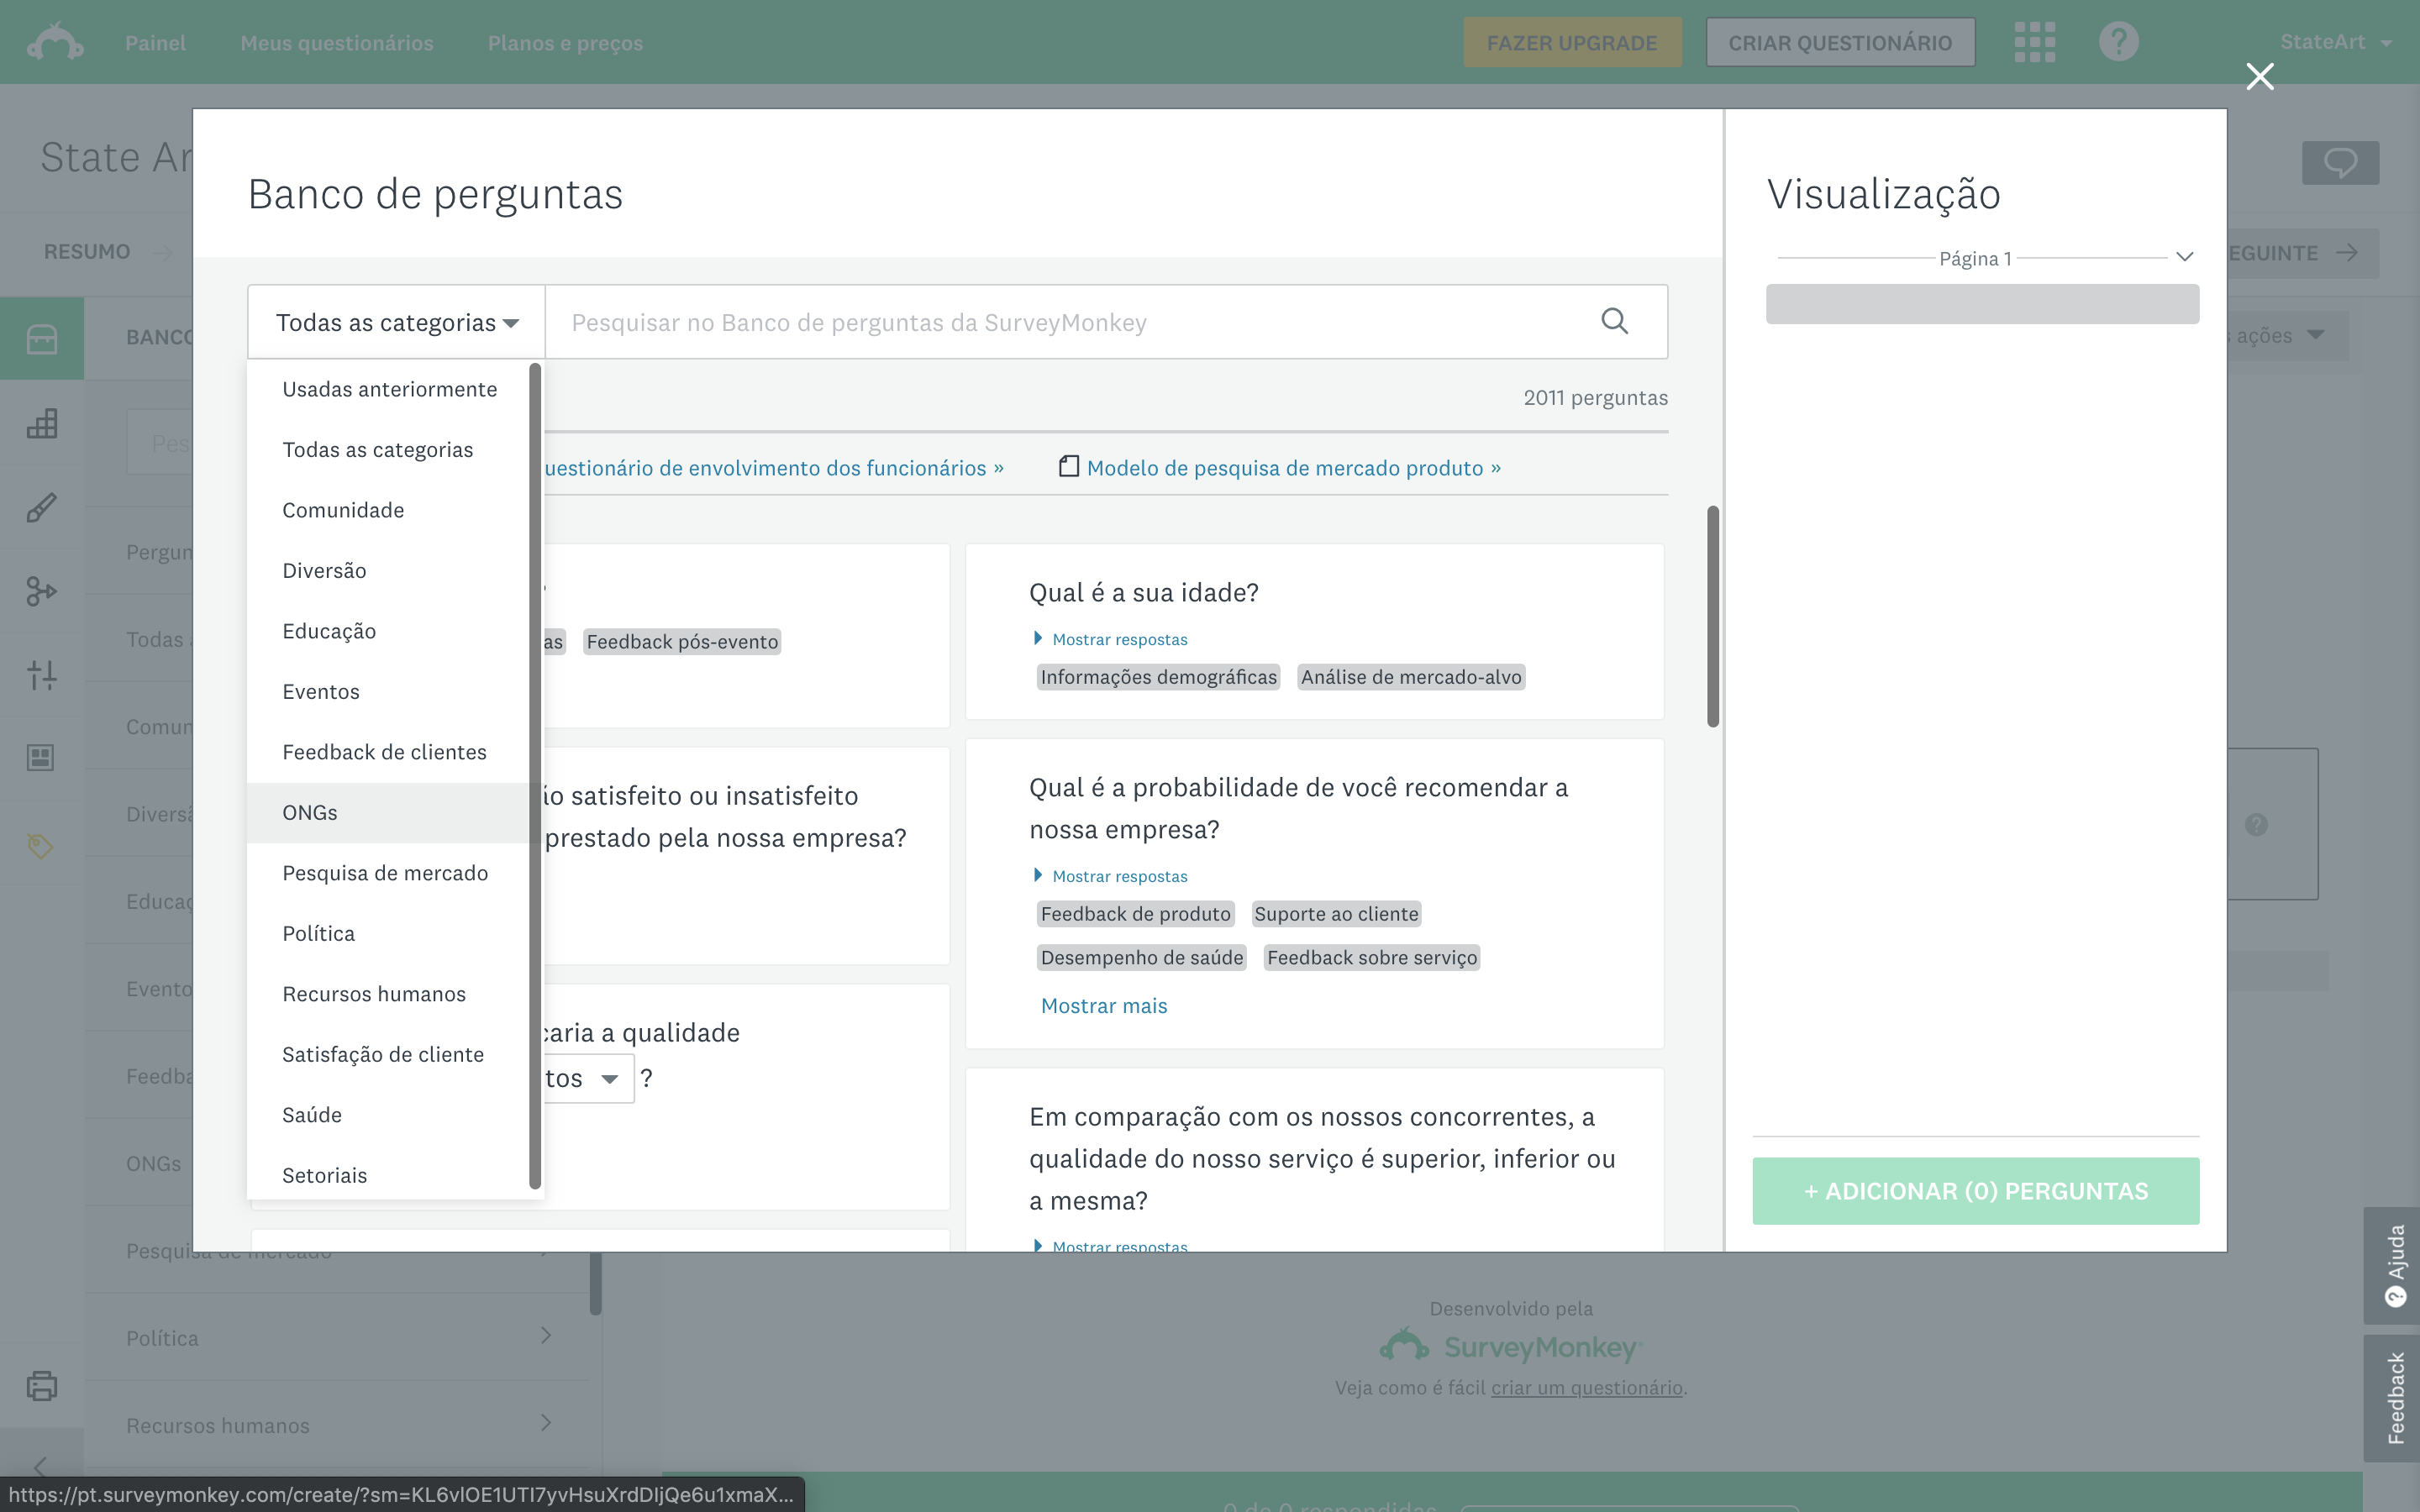
\includegraphics[width=1\textwidth]{img/sm/survey-form-bank1}
		\caption{SurveyMonkey - Perguntas Modelo }
		\label{fig:survey-form-banck1}
	\end{center}
\end{figure}

\newpage

São diversos os elementos que se podem adicionar ou arrastar para o formulário (i. e. perguntas, escolha múltipla, imagens...) como representado na Figura \ref{fig:surveymonkey-form-element} e há também um banco de perguntas modelo/recomendações já construídas, organizadas por categorias como podemos ver na Figura \ref{fig:survey-form-banck2} e \ref{fig:survey-form-banck1}.


\begin{figure}[ht!]
	\begin{center}
		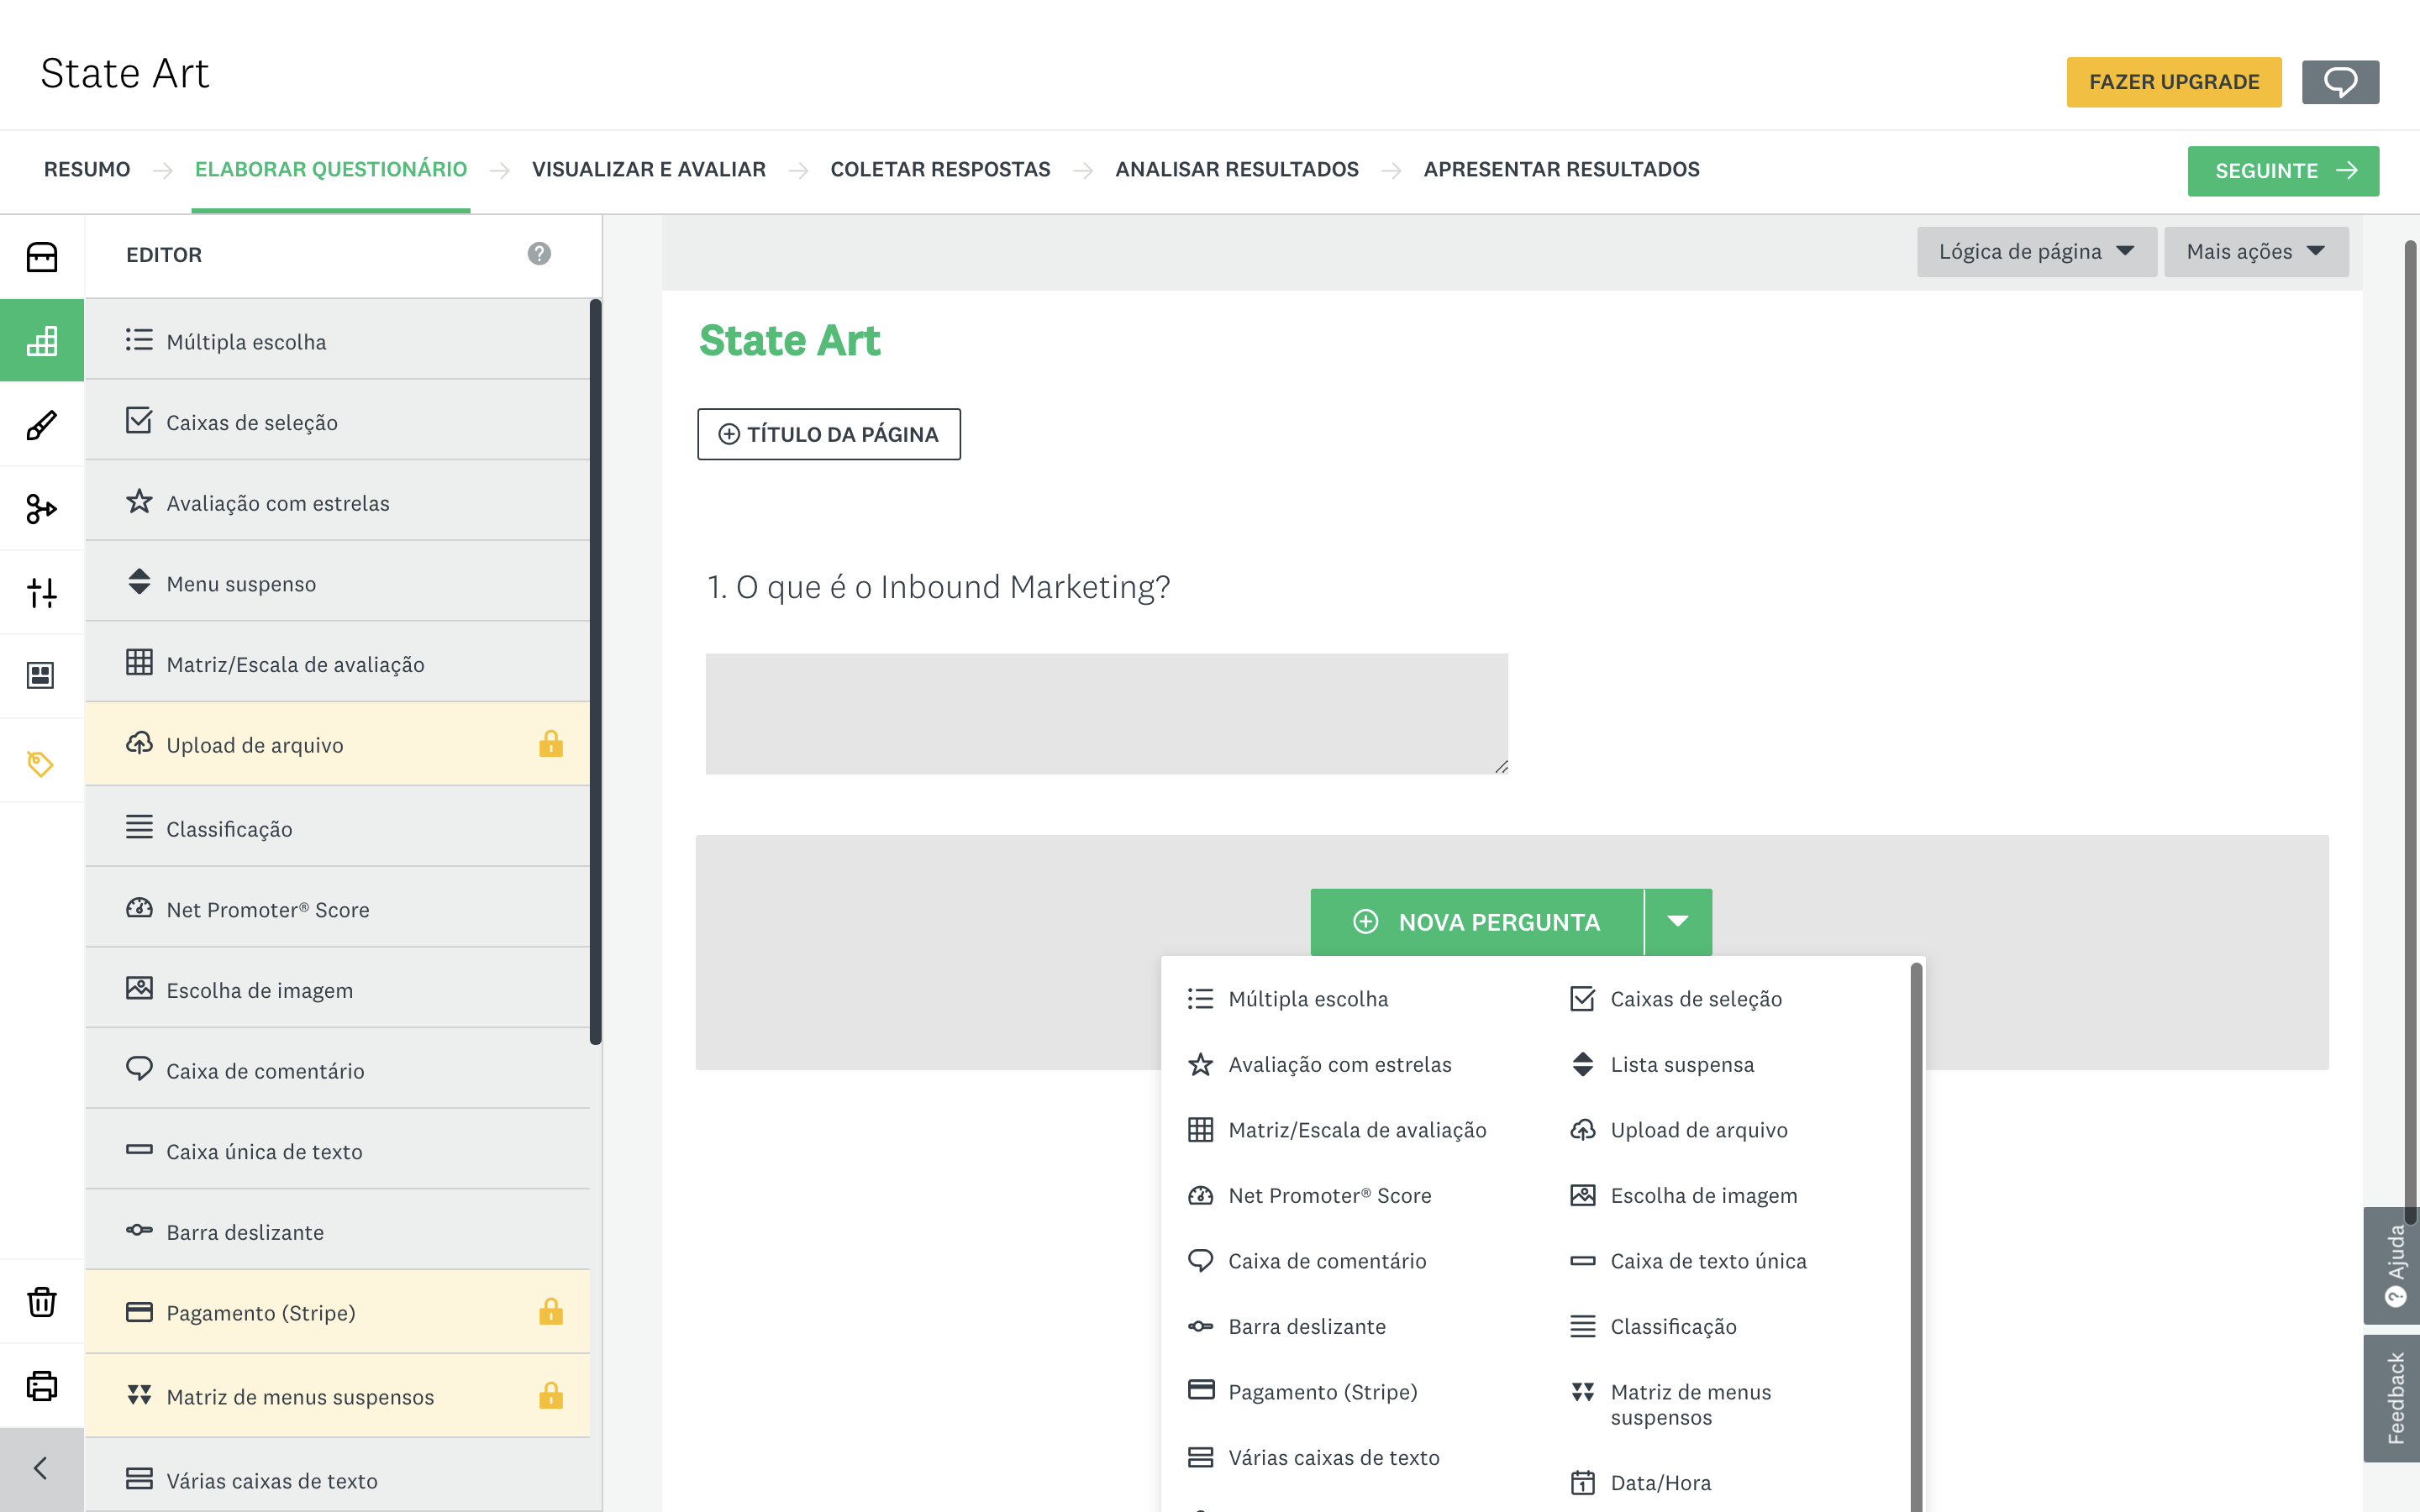
\includegraphics[width=1\textwidth]{img/sm/surveymonkey-form-element}
		\caption{SurveyMonkey - Elementos }
		\label{fig:surveymonkey-form-element}
	\end{center}
\end{figure}
\newpage

\begin{figure}[ht!]
	\begin{center}
		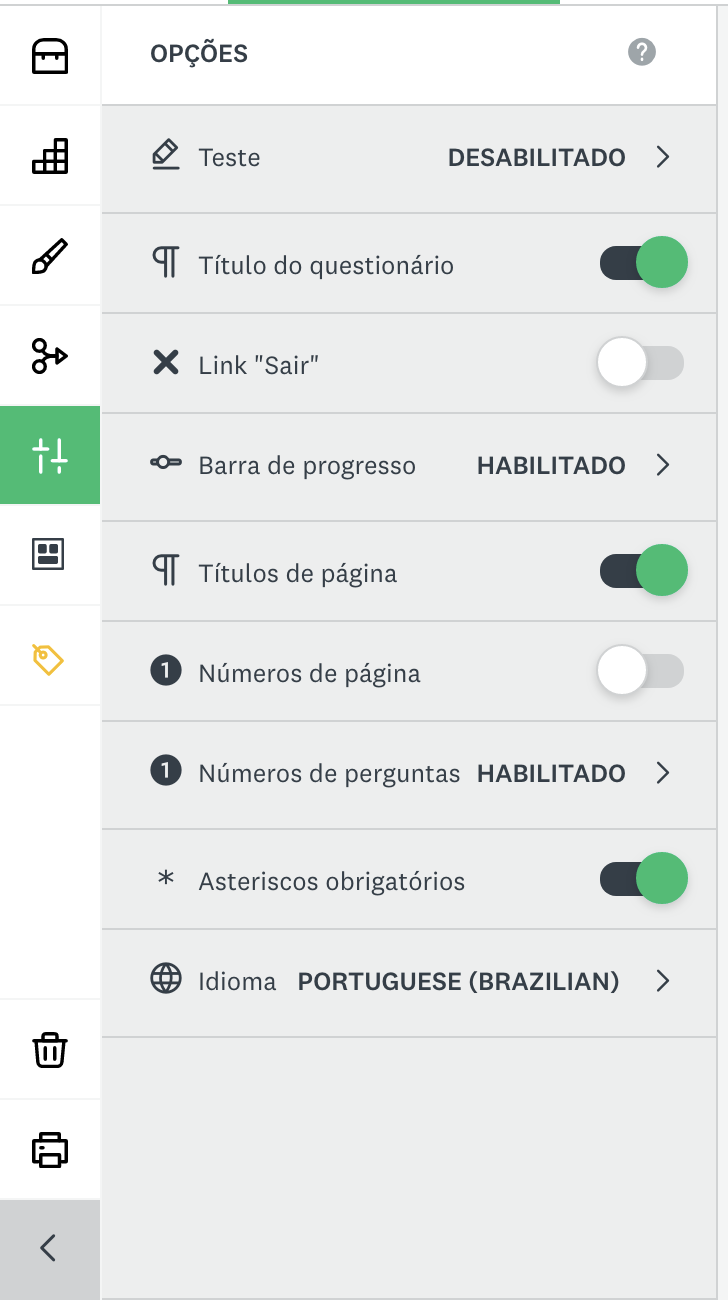
\includegraphics[height=.35\textheight]{img/sm/surveymonkey-form-opcoes}
		\caption{SurveyMonkey - Opções}
		\label{fig:surveymonkey-form-opcoes}
	\end{center}
\end{figure}

\begin{figure}[ht!]
	\begin{center}
		\begin{minipage}{0.45\textwidth}
			\begin{center}
				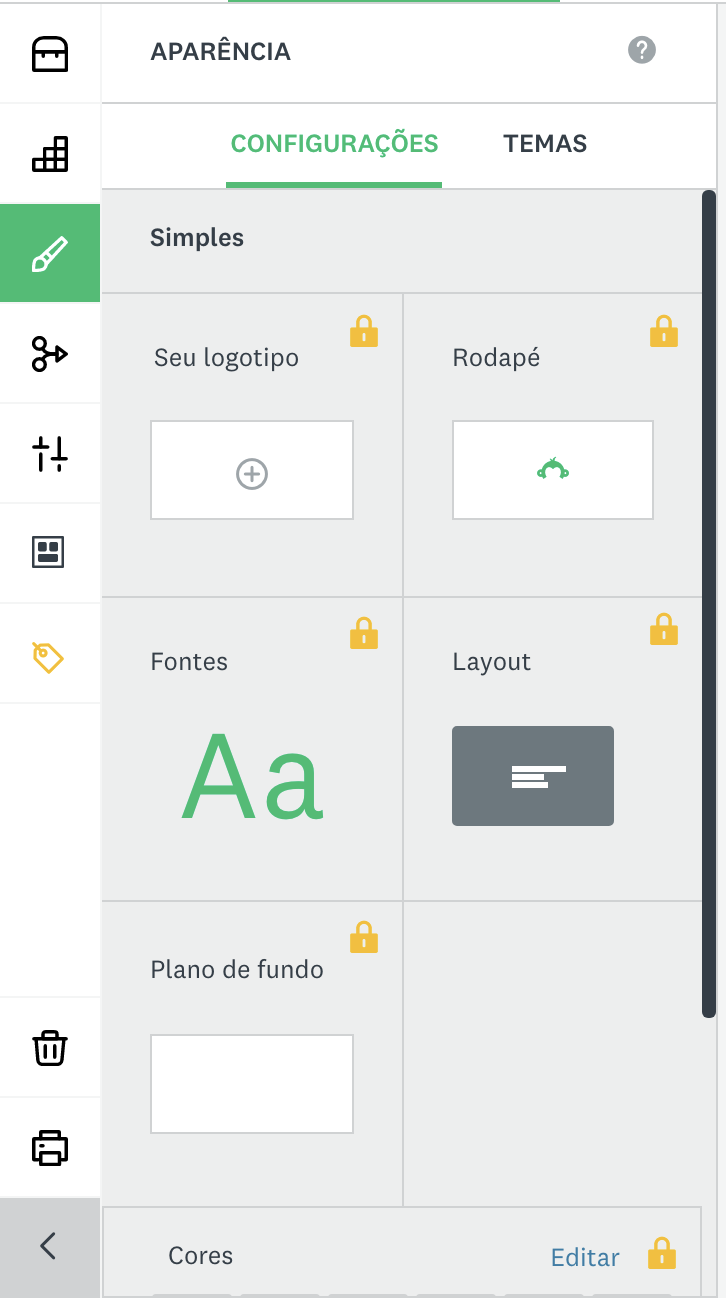
\includegraphics[height=.35\textheight]{img/sm/surveymonkey-form-aparencia}
				\caption{SurveyMonkey - Aparência}
				\label{fig:surveymonkey-form-aparencia}
			\end{center}
		\end{minipage}
		\hspace{1cm}
		\begin{minipage}{0.45\textwidth}
			\begin{center}
				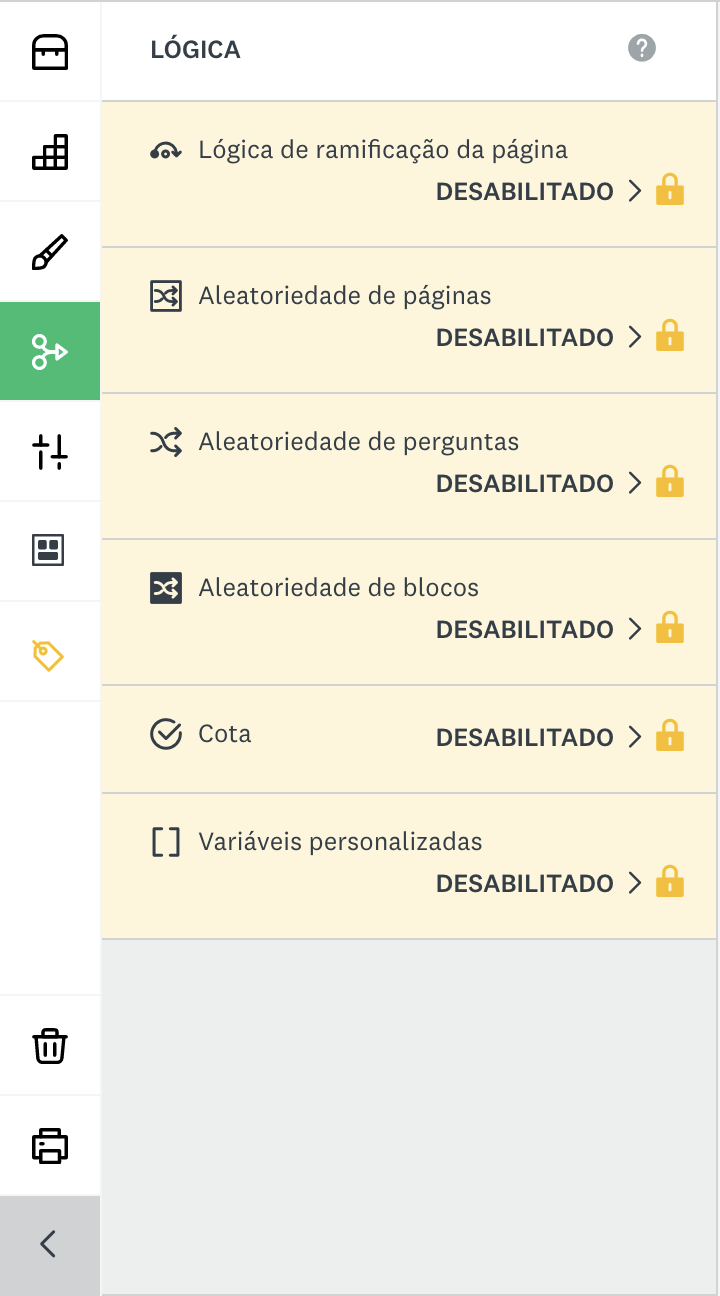
\includegraphics[height=.35\textheight]{img/sm/surveymonkey-form-logica}
				\caption{SurveyMonkey - Lógica}
				\label{fig:surveymonkey-form-logica}
			\end{center}
		\end{minipage}
	\end{center}
\end{figure}

O SurveyMonkey permite também realizar algumas operações de personalização do formulário. Nas Figuras \ref{fig:surveymonkey-form-opcoes}, \ref{fig:surveymonkey-form-aparencia} e \ref{fig:surveymonkey-form-logica} estão representadas as opções, aparência e lógica do formulário, respetivamente, que permite customizar formulários ao público alvo. 
Depois de realizado o formulário esta plataforma permite a visualização do mesmo, em diferentes tipos de dispositivos, como se pode ver nas Figuras \ref{fig:surveymonkey-form-test-pc} e \ref{fig:surveymonkey-form-test-phone}, para verificar se tudo está conforme planeado para se poder prosseguir para a recolha de dados. 
\newpage

\begin{figure}[ht!]
	\begin{center}
		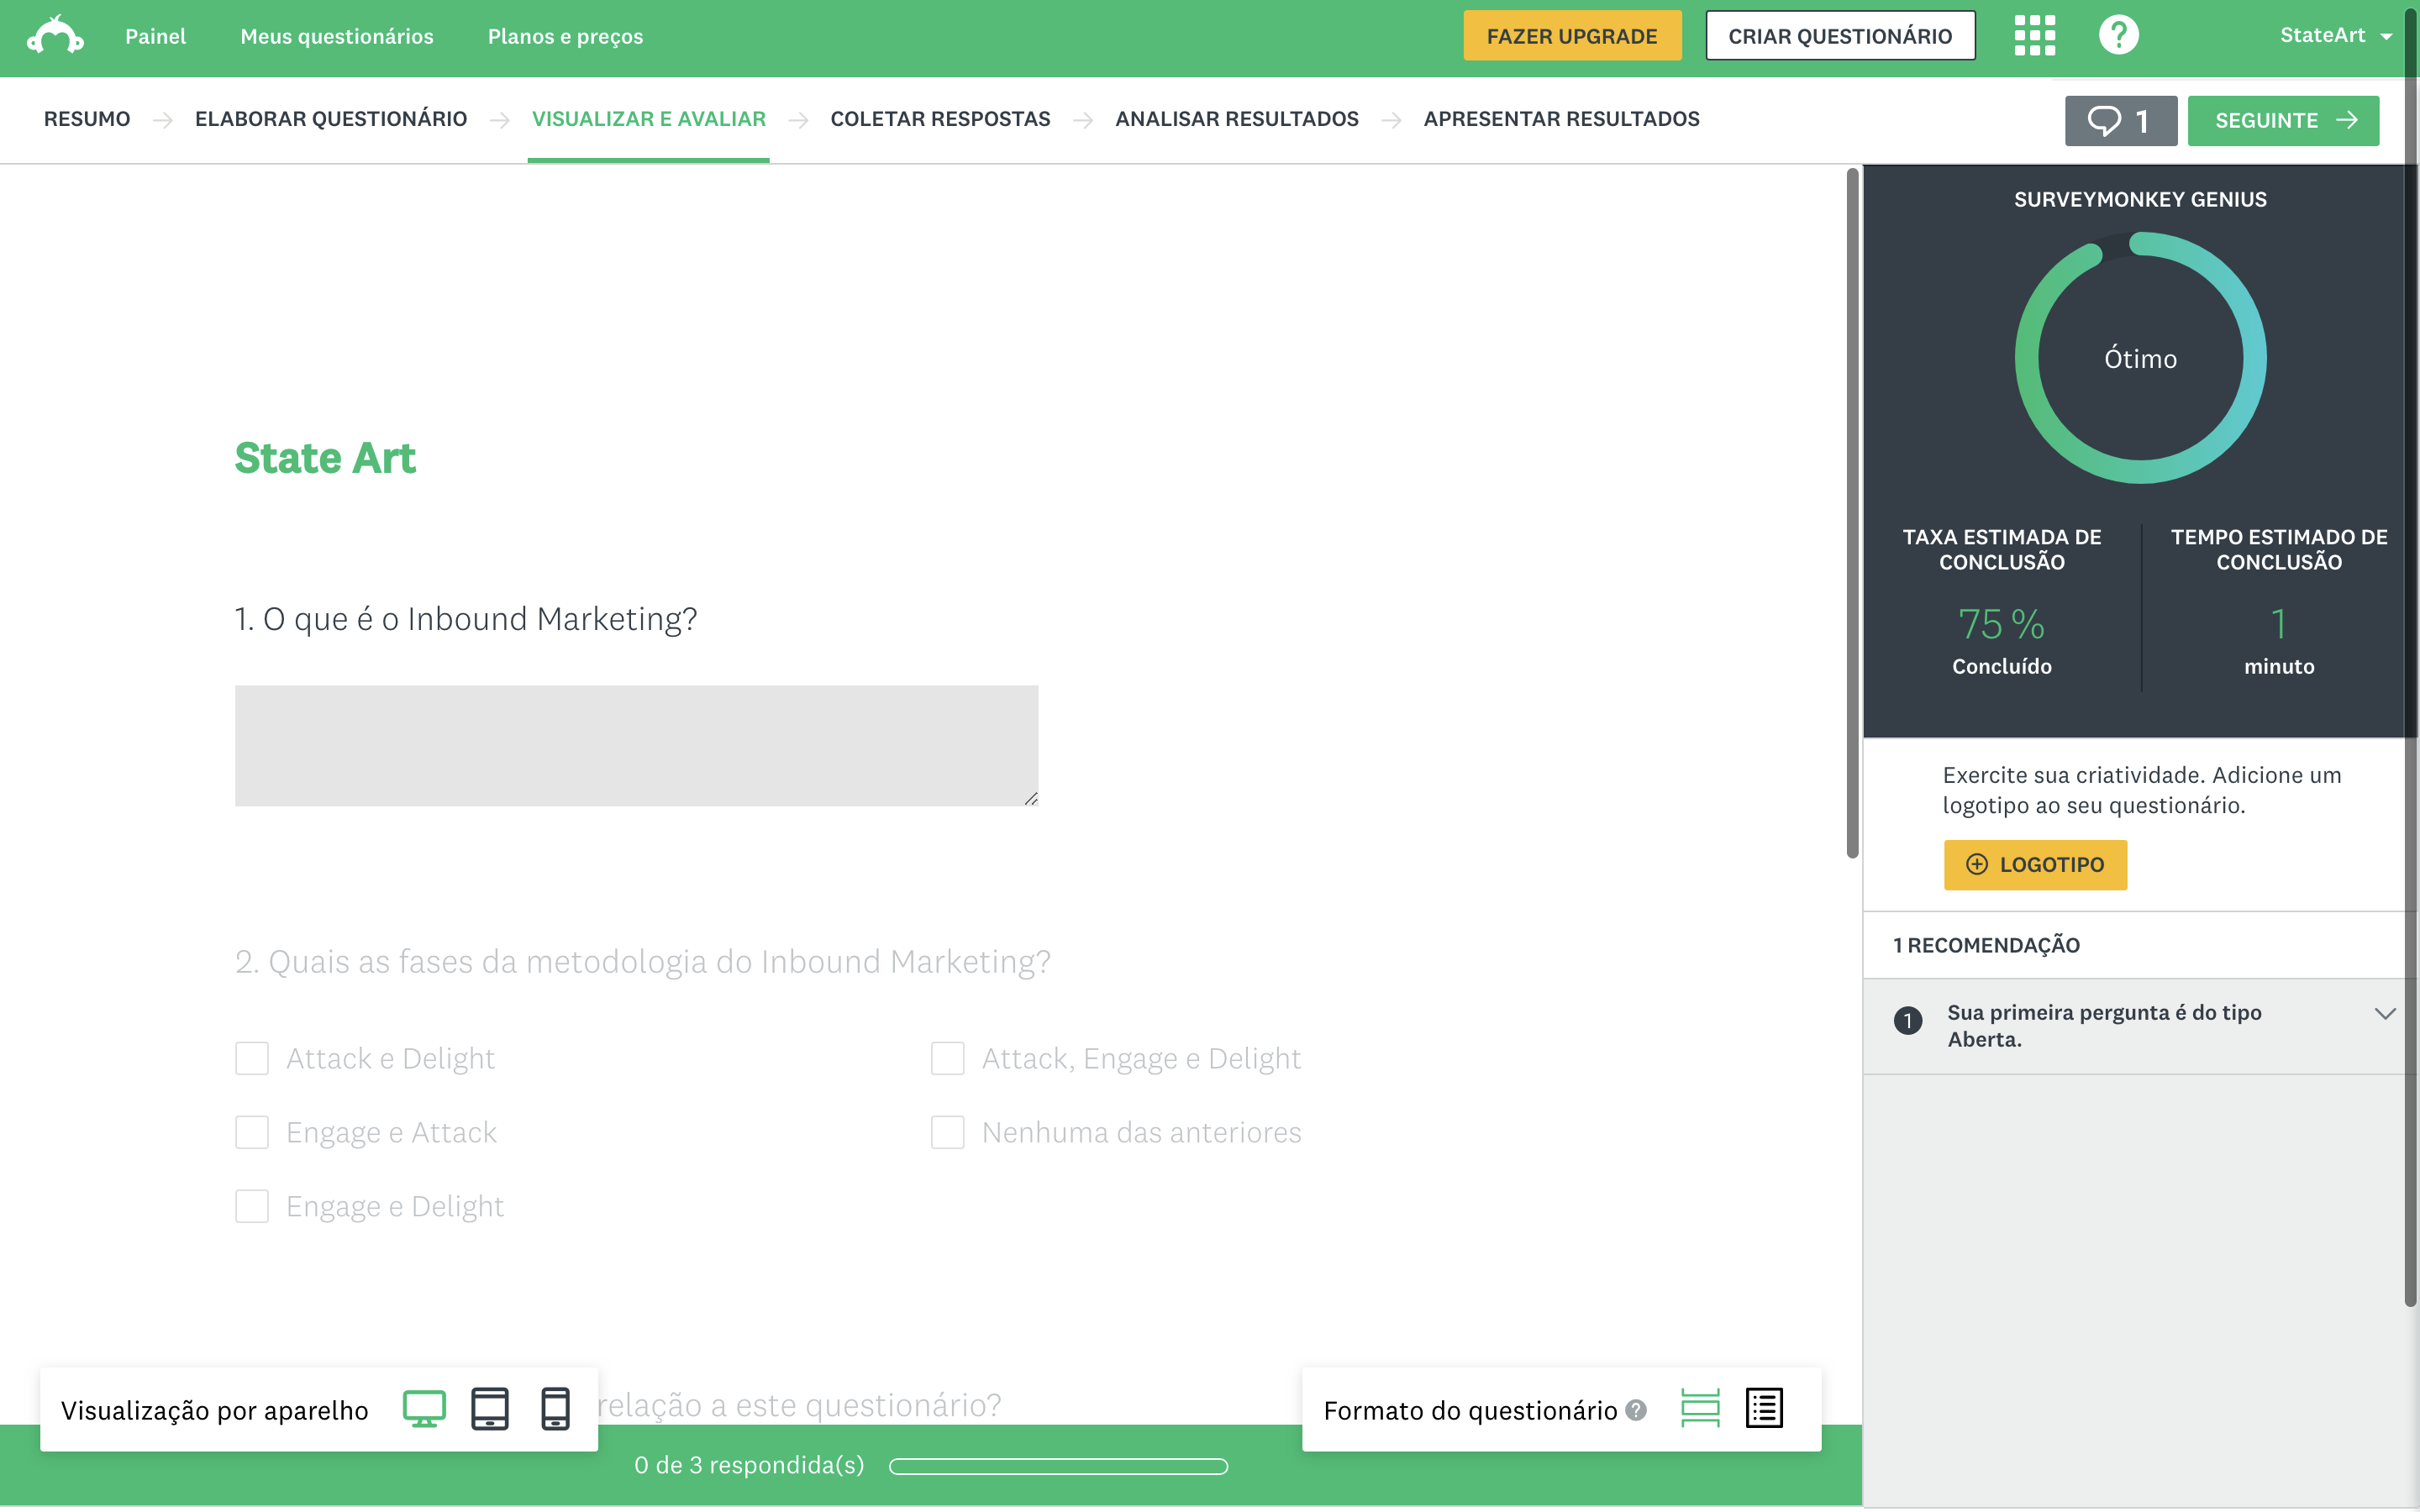
\includegraphics[width=1\textwidth]{img/sm/surveymonkey-form-test-pc}
		\caption{SurveyMonkey - Visualização do formulário em computador }
		\label{fig:surveymonkey-form-test-pc}
	\end{center}
\end{figure}

\begin{figure}[ht!]
	\begin{center}
		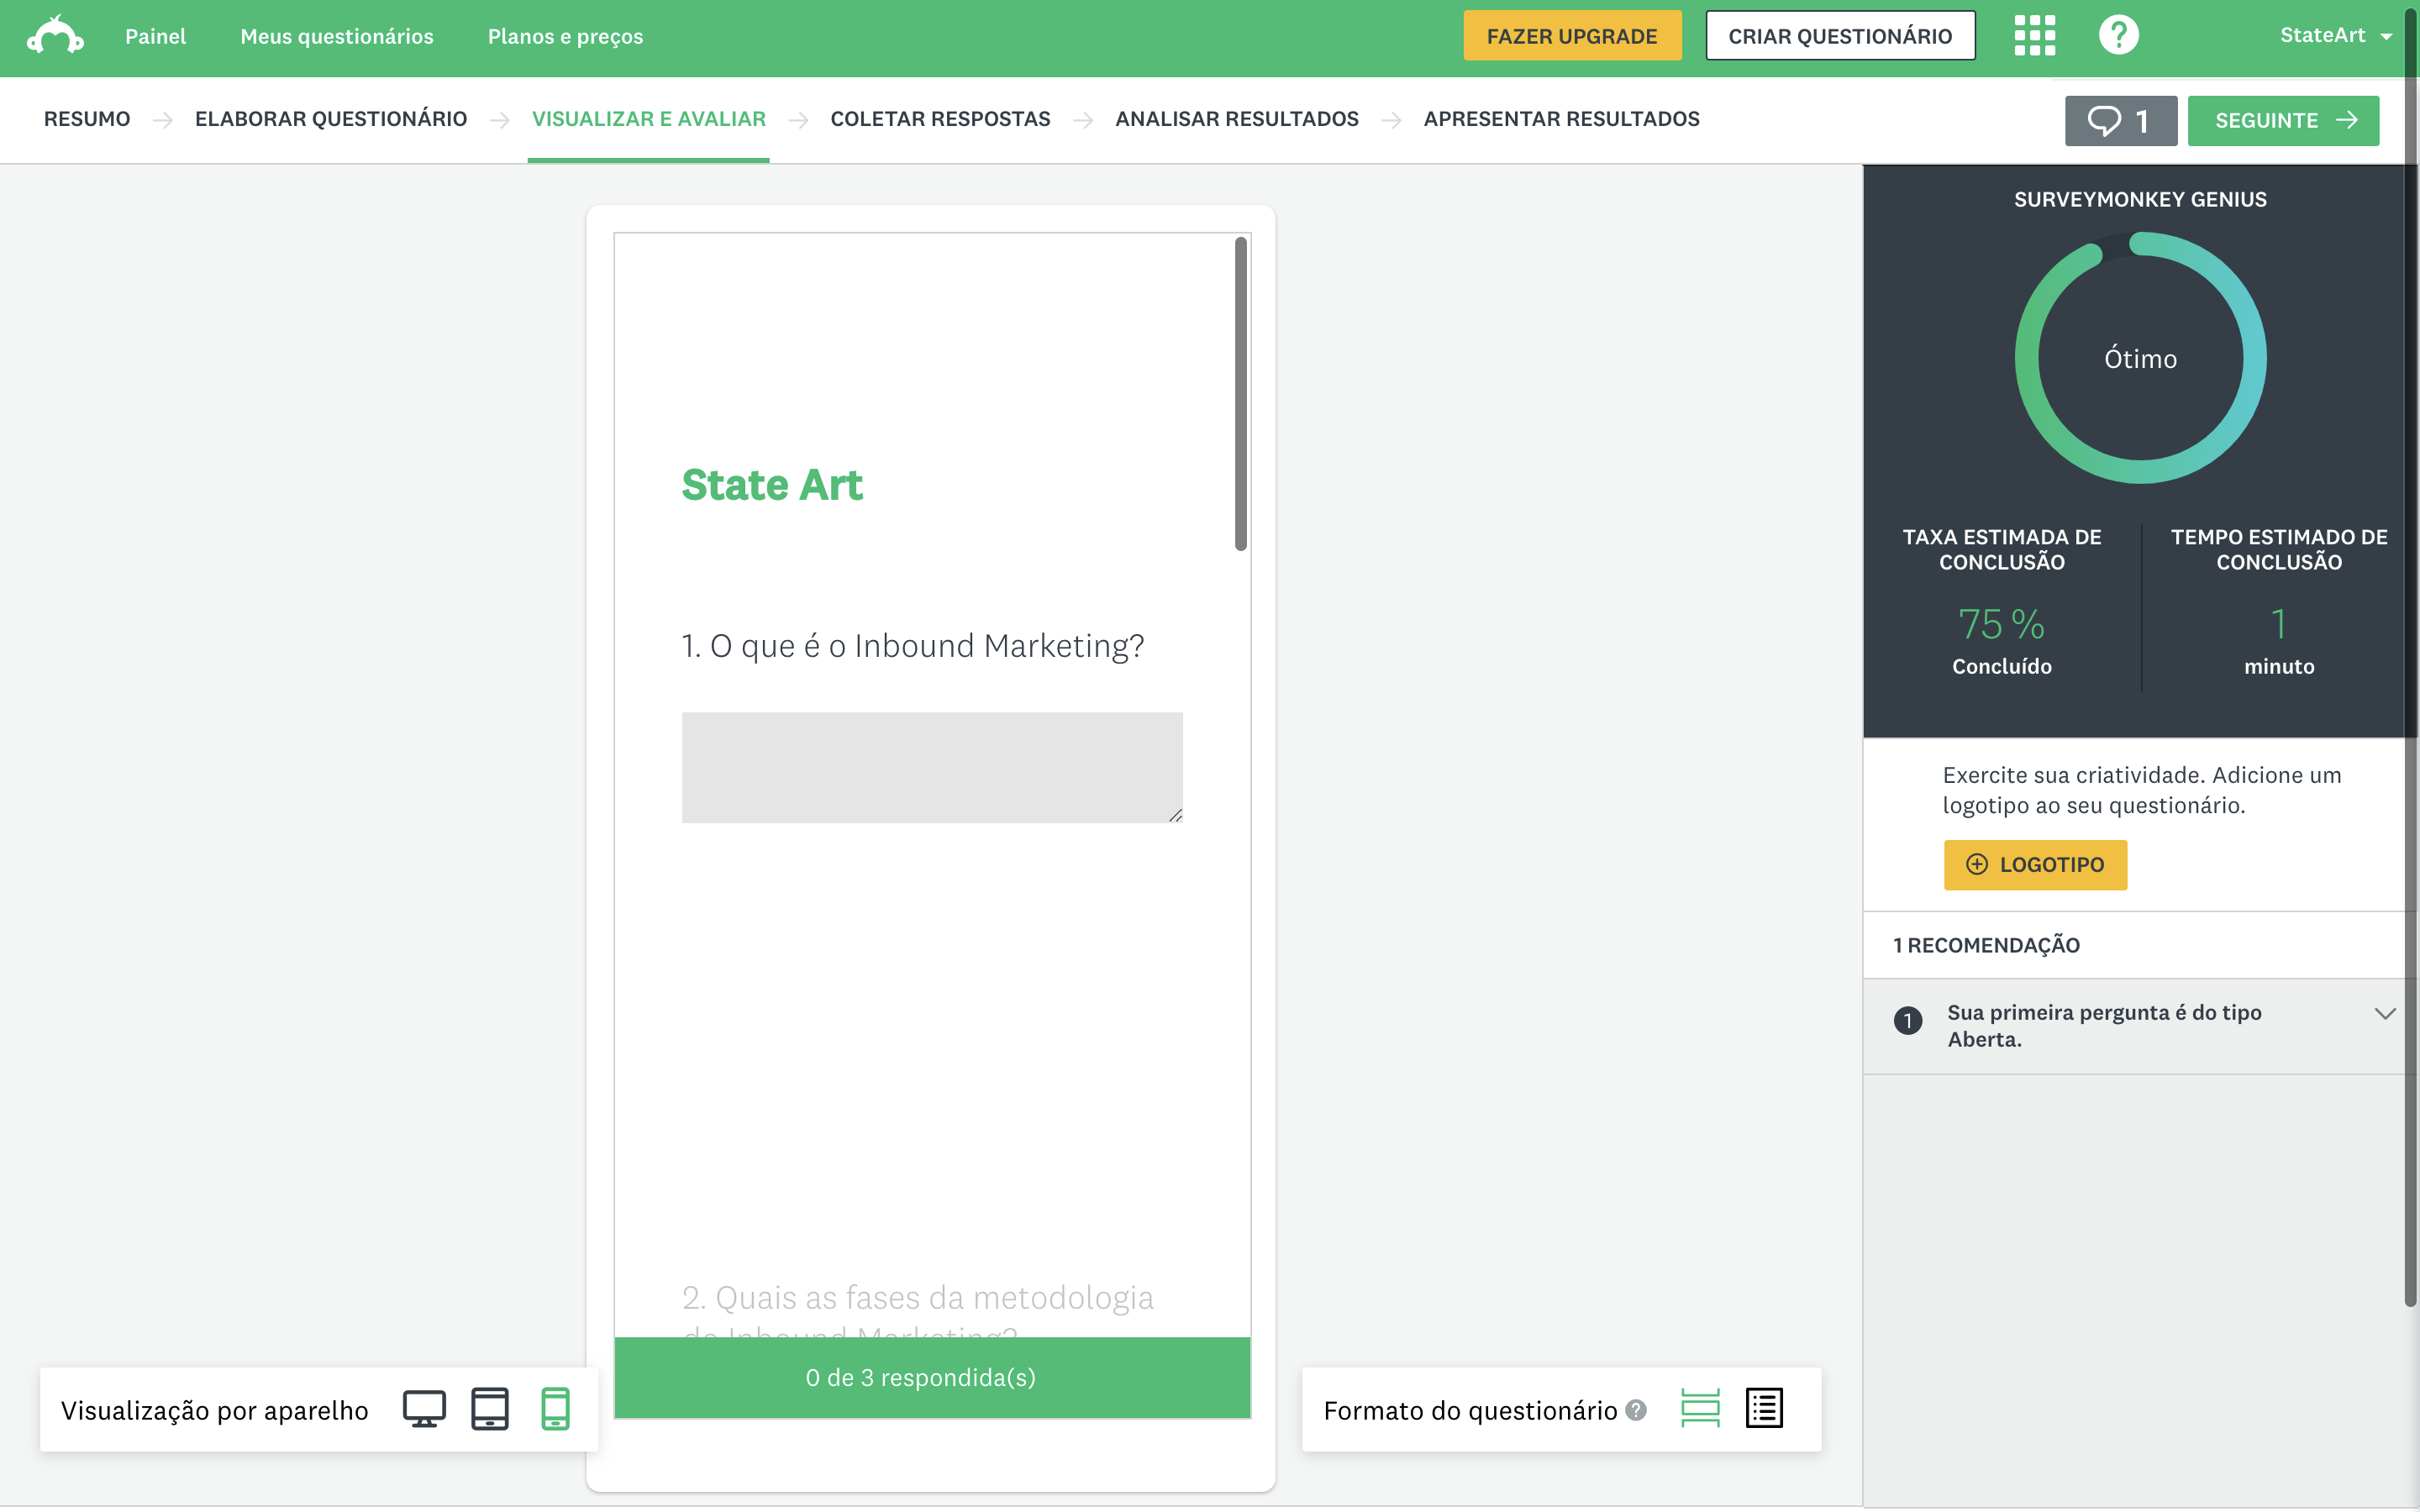
\includegraphics[width=1\textwidth]{img/sm/surveymonkey-form-test-phone}
		\caption{SurveyMonkey - Visualização do formulário em smartphone }
		\label{fig:surveymonkey-form-test-phone}
	\end{center}
\end{figure}

Depois de garantir que o formulário foi construído como desejado a plataforma fornece vários meios pelo qual se pode partilhar/enviar o formulário, como listado na Figura \ref{fig:surveymonkey-form-share}.

\newpage

\begin{figure}[ht!]
	\begin{center}
		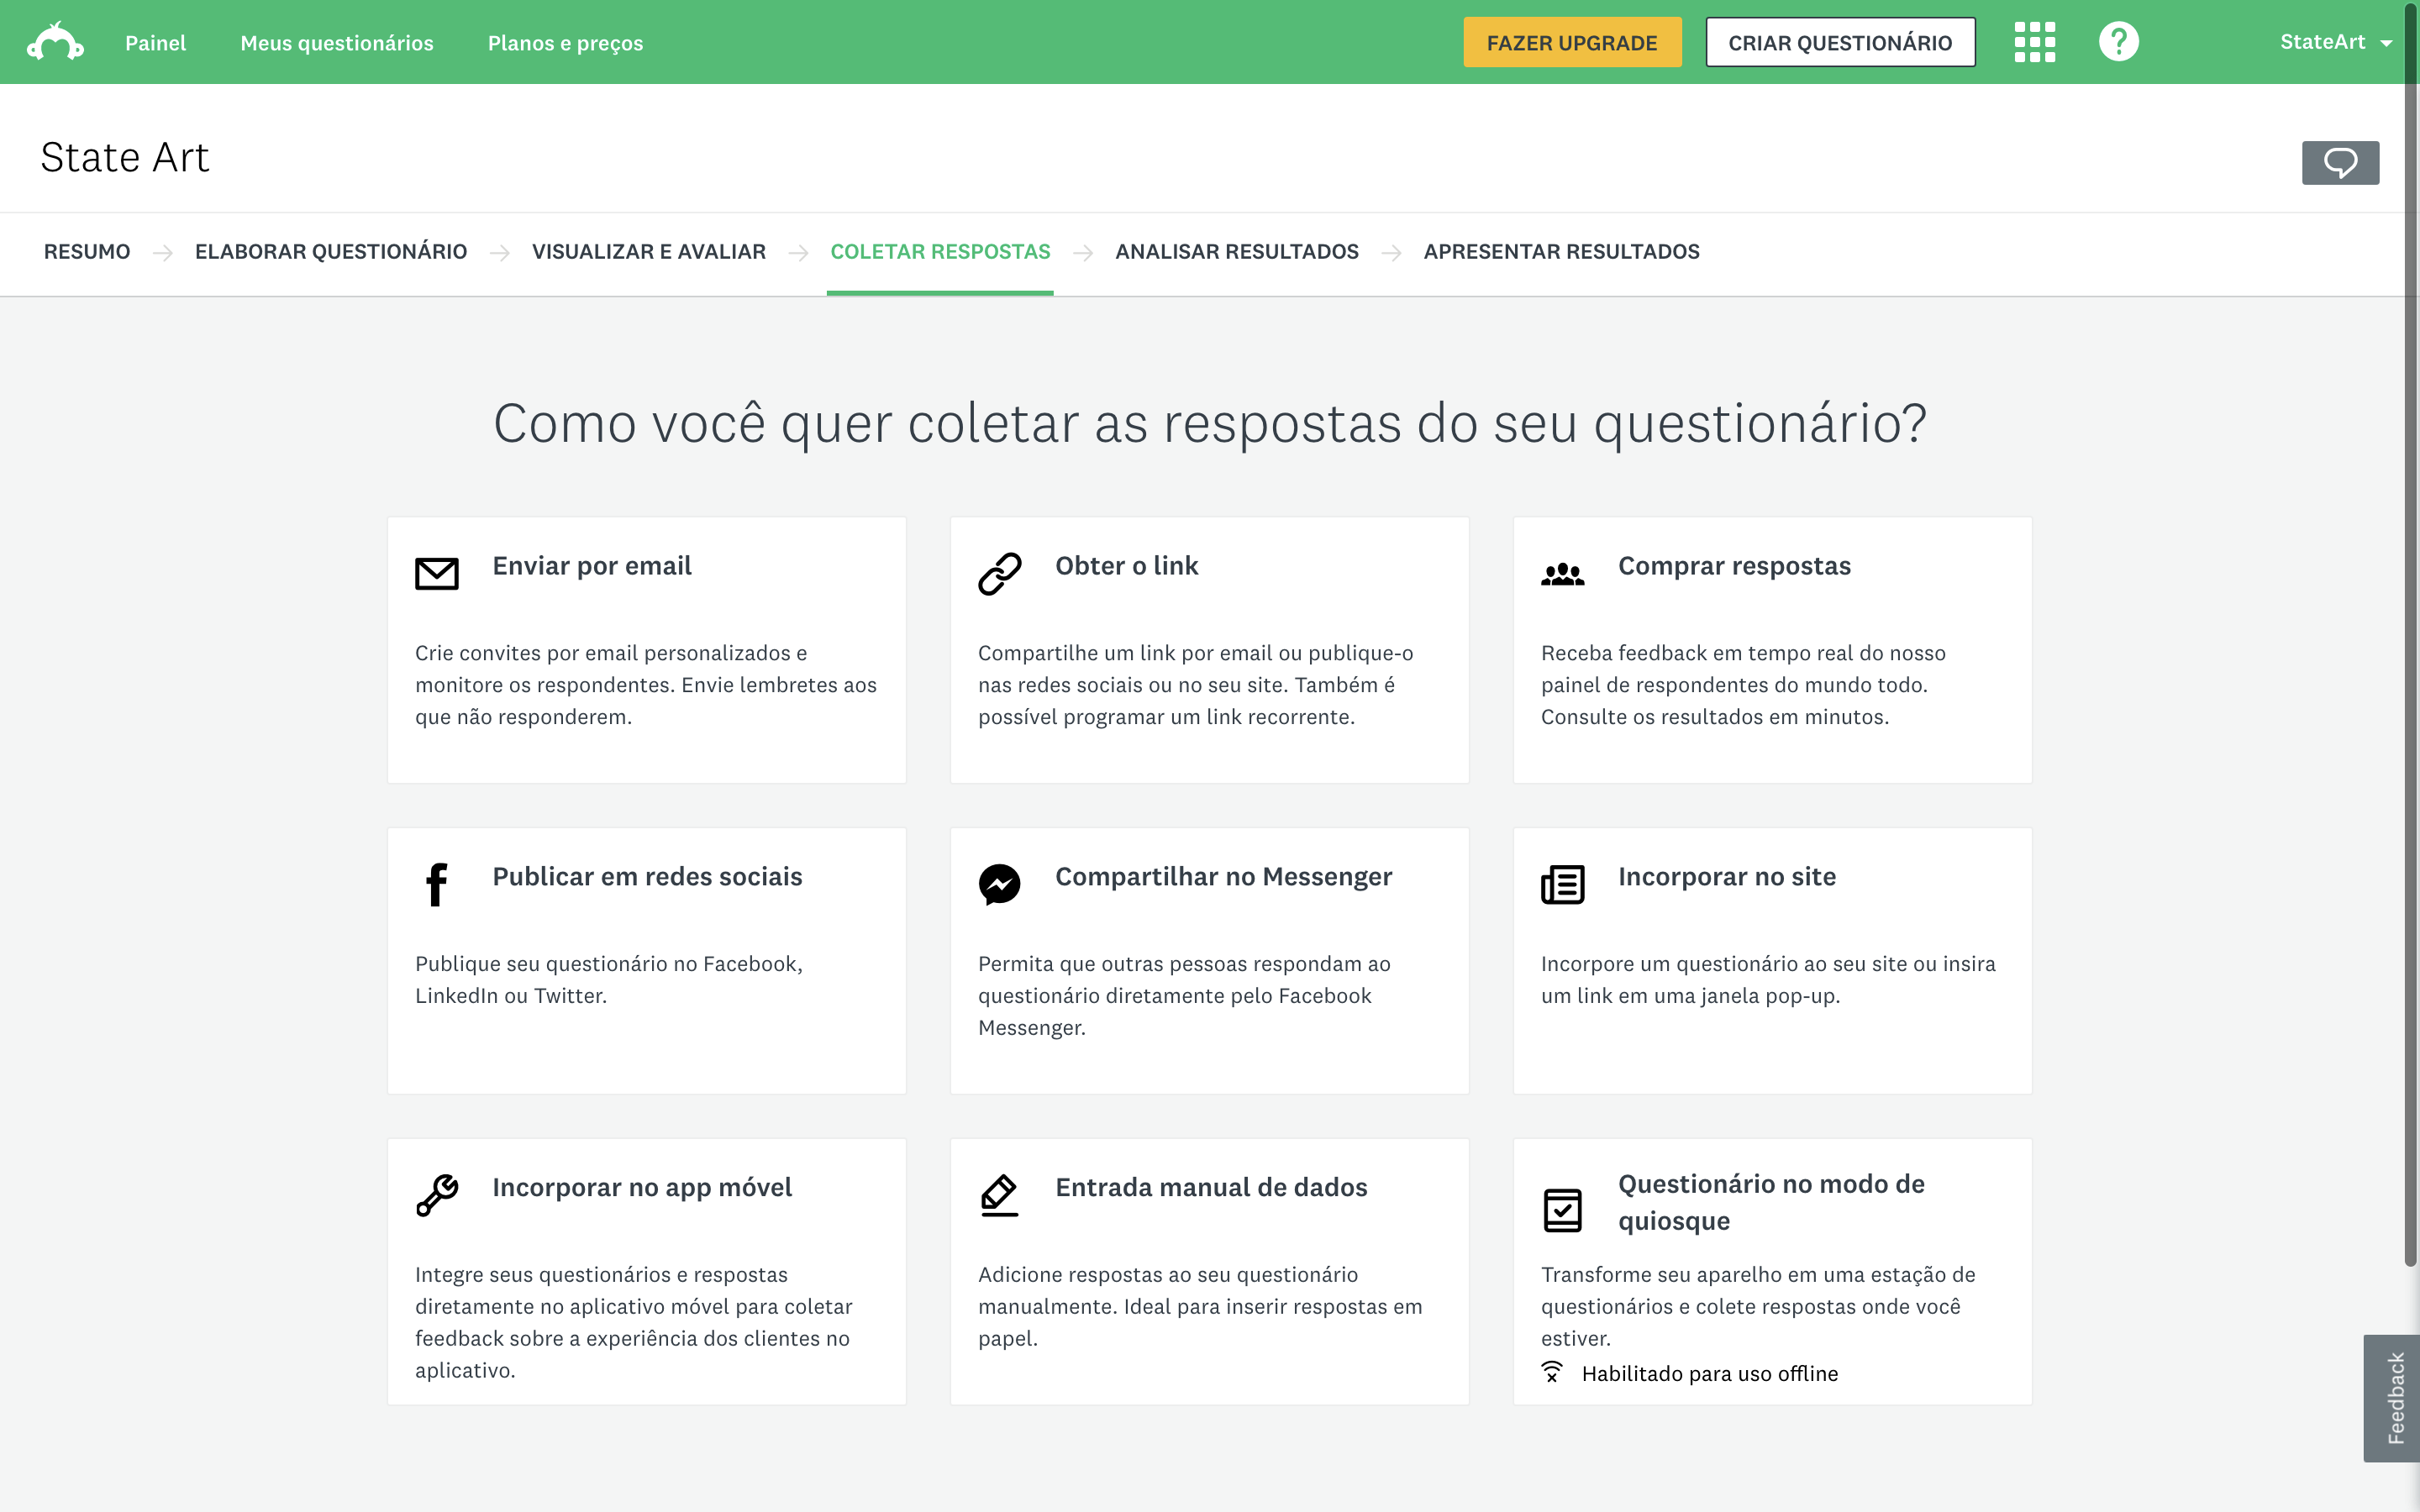
\includegraphics[width=1\textwidth]{img/sm/surveymonkey-form-share}
		\caption{SurveyMonkey - Método de partilha do formulário }
		\label{fig:surveymonkey-form-share}
	\end{center}
\end{figure}

Na análise de resultados, é necessário actualizar a página ou aplicar um filtro para que os gráficos e as estatísticas sejam actualizadas. 
O mesmo se passa na página que pode ser gerada para partilhar o sumário dos dados recolhidos, através do formulário. 
Para aplicar um filtro é necessário escolher o tipo de filtro e os elementos ao qual queremos aplicar o filtro como podemos ver nas Figuras \ref{fig:surveymonkey-form-filtro} e \ref{fig:surveymonkey-form-filtro1}. 


\begin{figure}[ht!]
	\begin{center}
		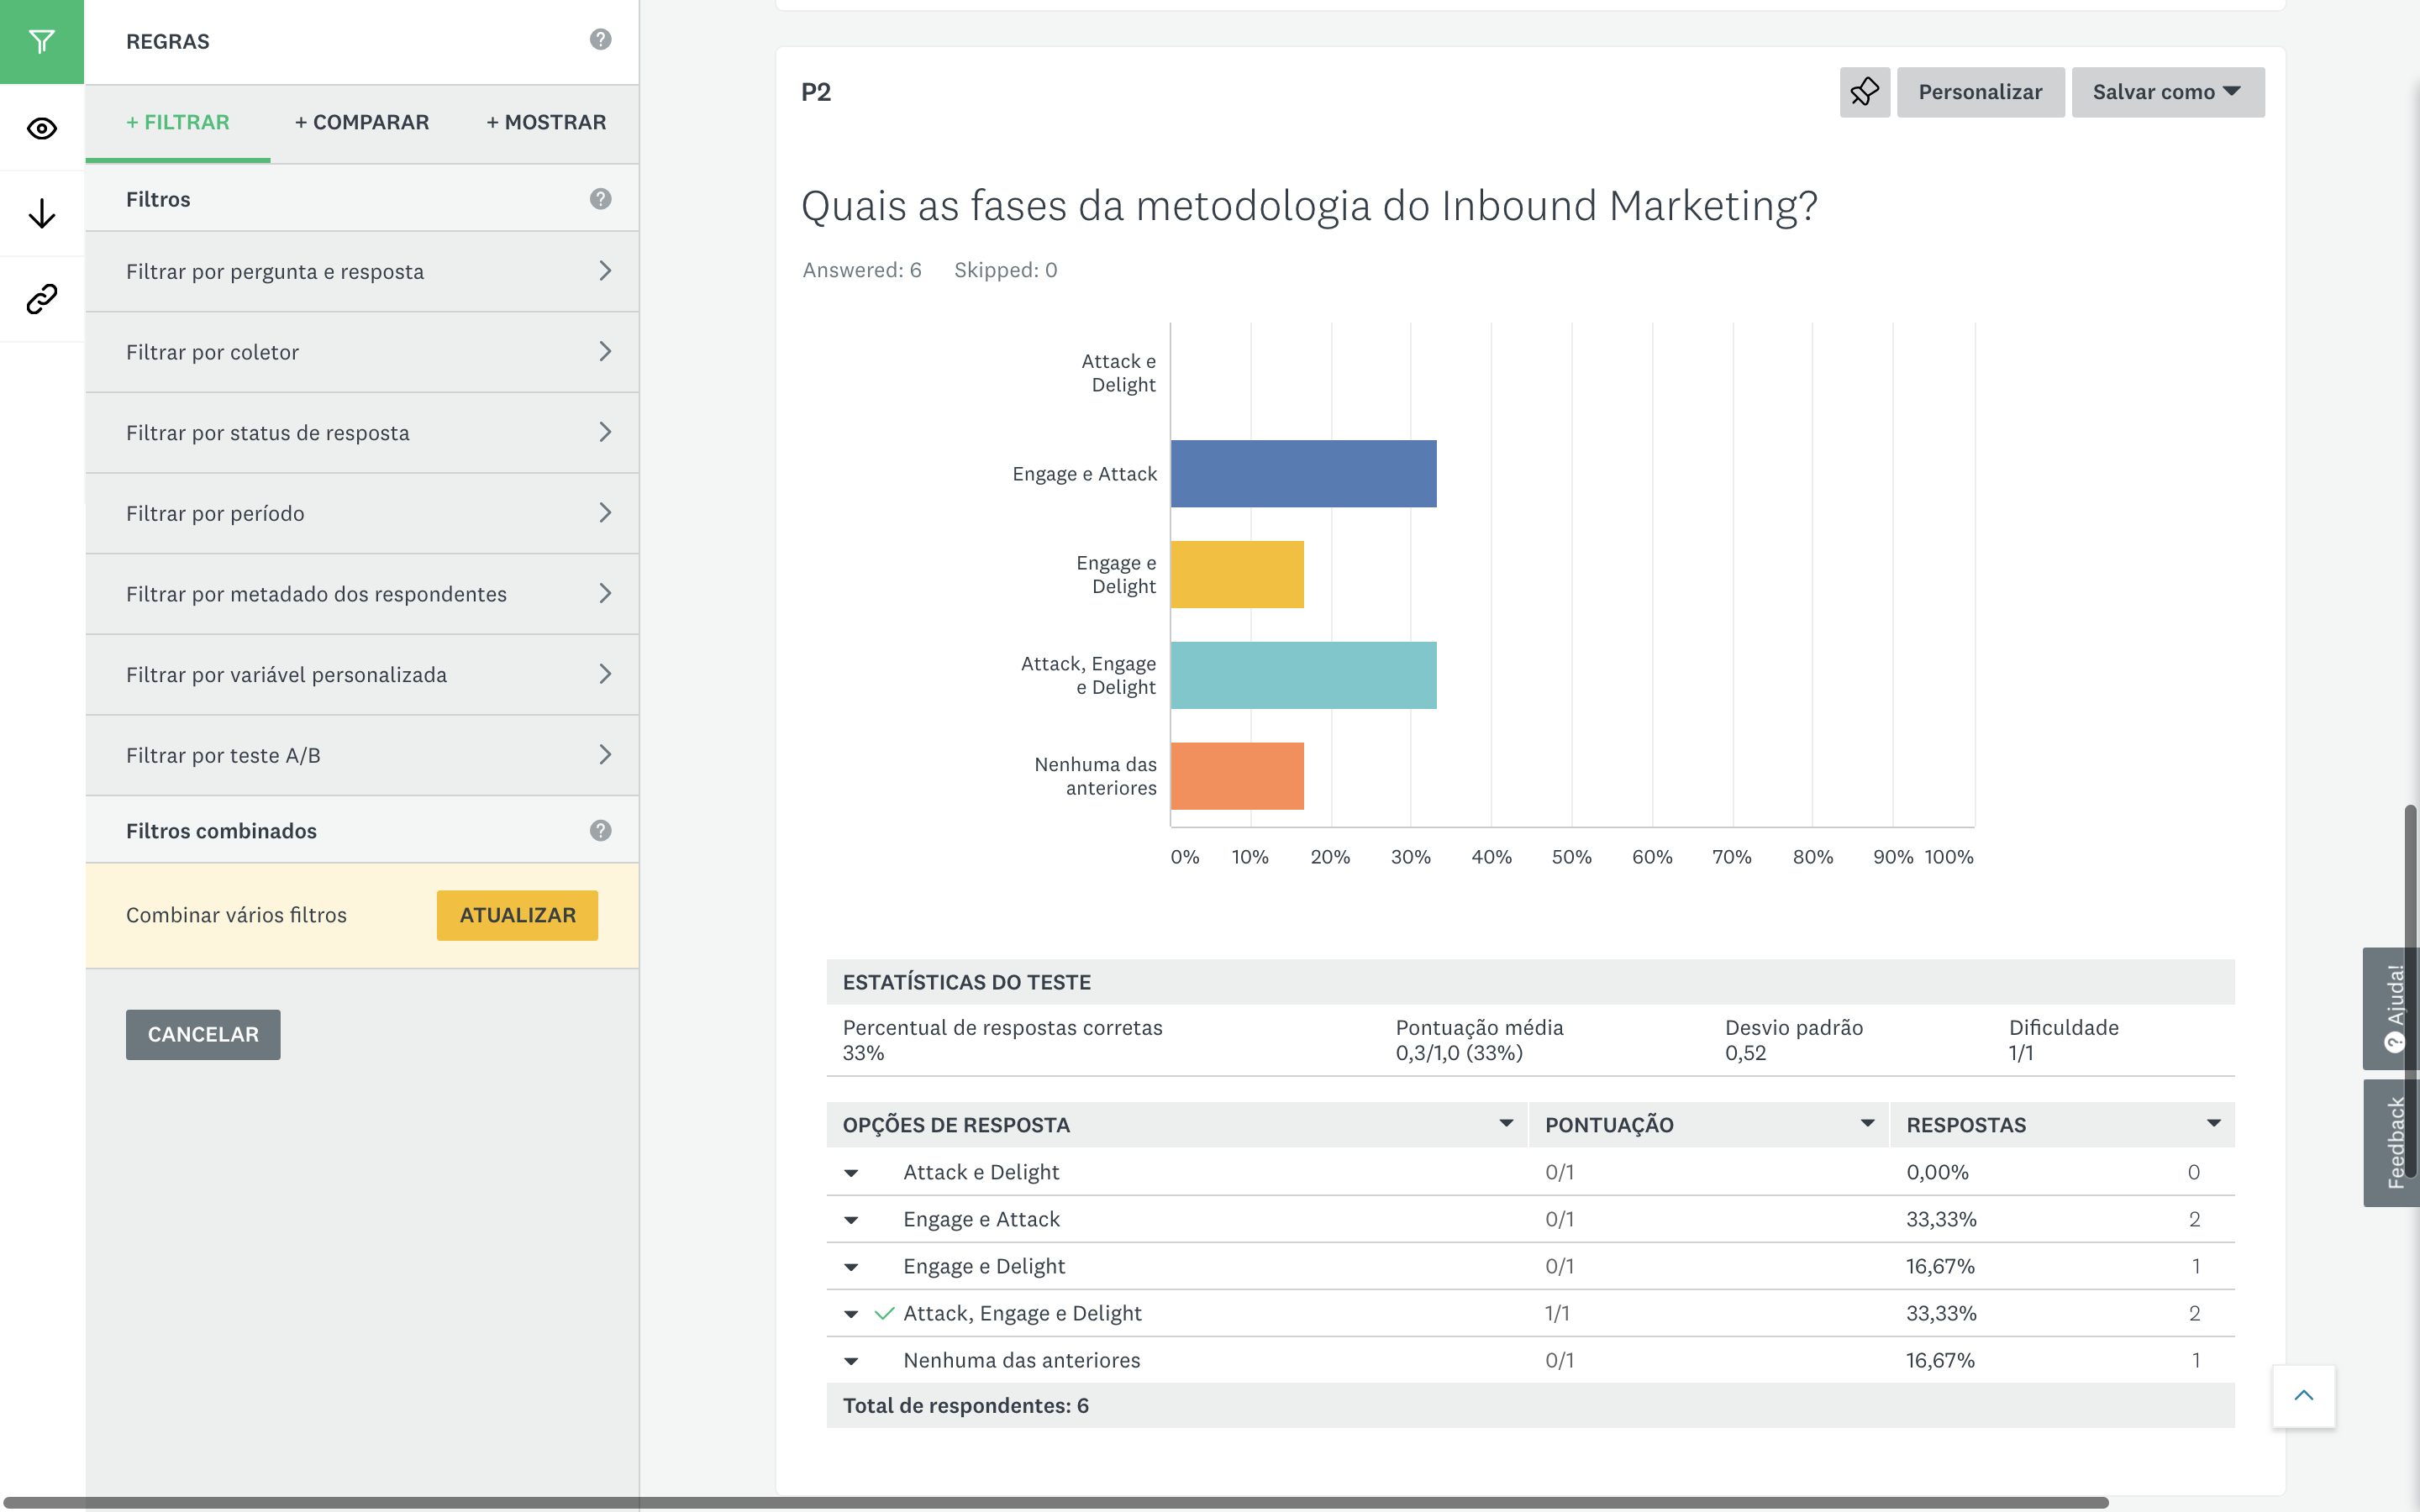
\includegraphics[width=1\textwidth]{img/sm/surveymonkey-form-filtro}
		\caption{SurveyMonkey - Tipos de Filtros }
		\label{fig:surveymonkey-form-filtro}
	\end{center}
\end{figure}



\begin{figure}[ht!]
	\begin{center}
		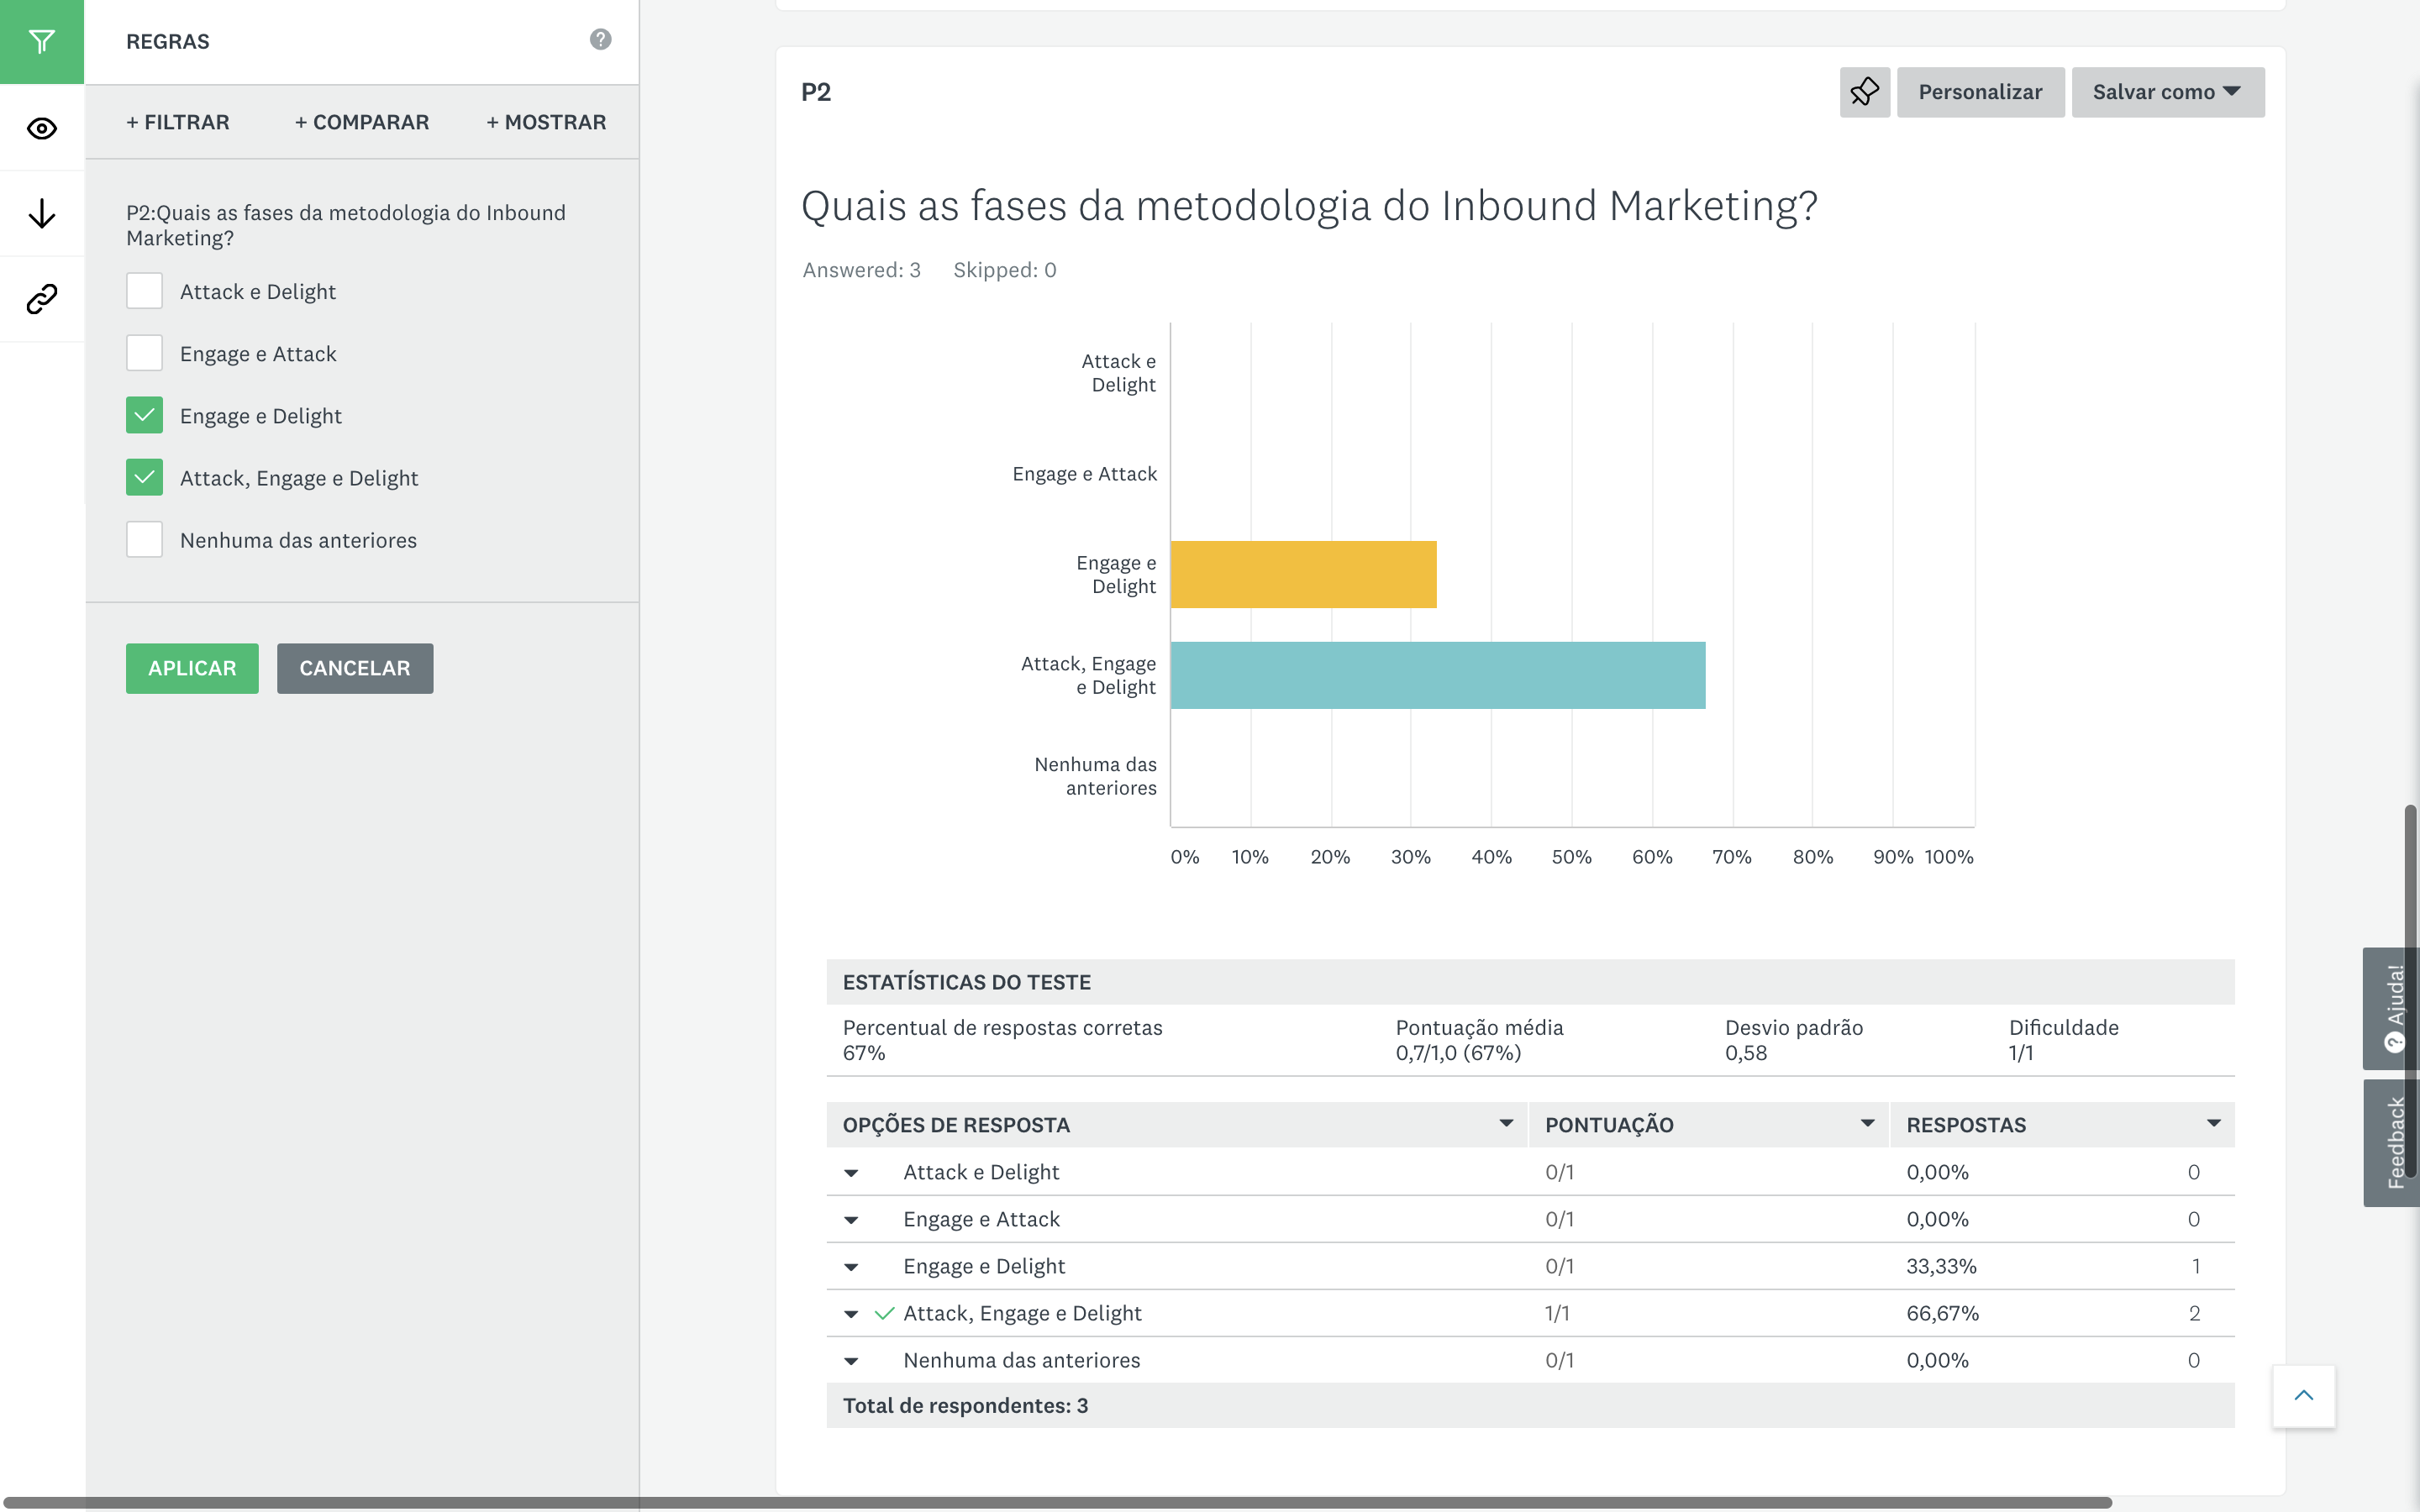
\includegraphics[width=1\textwidth]{img/sm/surveymonkey-form-filtro1}
		\caption{SurveyMonkey - Filtro aplicado na pergunta 2 }
		\label{fig:surveymonkey-form-filtro1}
	\end{center}
\end{figure}

Para finalizar a plataforma SurveyMonkey tem ainda uma funcionalidade que, através da representação dos dados numa linha temporal, permite o utilizador perceber as tendências dos dados.

\section{Typeform}
\label{typeform}

O Typeform é uma plataforma \acrshort{saas} de criação de formulários online. É uma empresa que afirma resolver o problema dos formulários e inquéritos aborrecidos e tem também como proposta de valor o facto de conseguir criar formulários e inquéritos sem ter que programar uma única linha de código. Esta plataforma permite recolher informações do público alvo através de formulários e inquéritos personalizados e no final visualizar estes dados. 

O Typeform disponibiliza um pacote gratuito, contudo, é necessário criar conta de utilizador, para aceder às funcionalidades da plataforma. Tanto o registro como o início de sessão pode ser feito através da \acrfull{api} do Google.

Como podemos ver na Figura \ref{fig:tf-dashboard}, no painel de controlo, podemos criar várias áreas de trabalho. Cada área de trabalho é independente e todos os formulários e inquéritos que forem adicionados ao mesmo podem ser partilhados com mais do que uma pessoa.

\clearpage

\begin{figure}[ht!]
	\begin{center}
		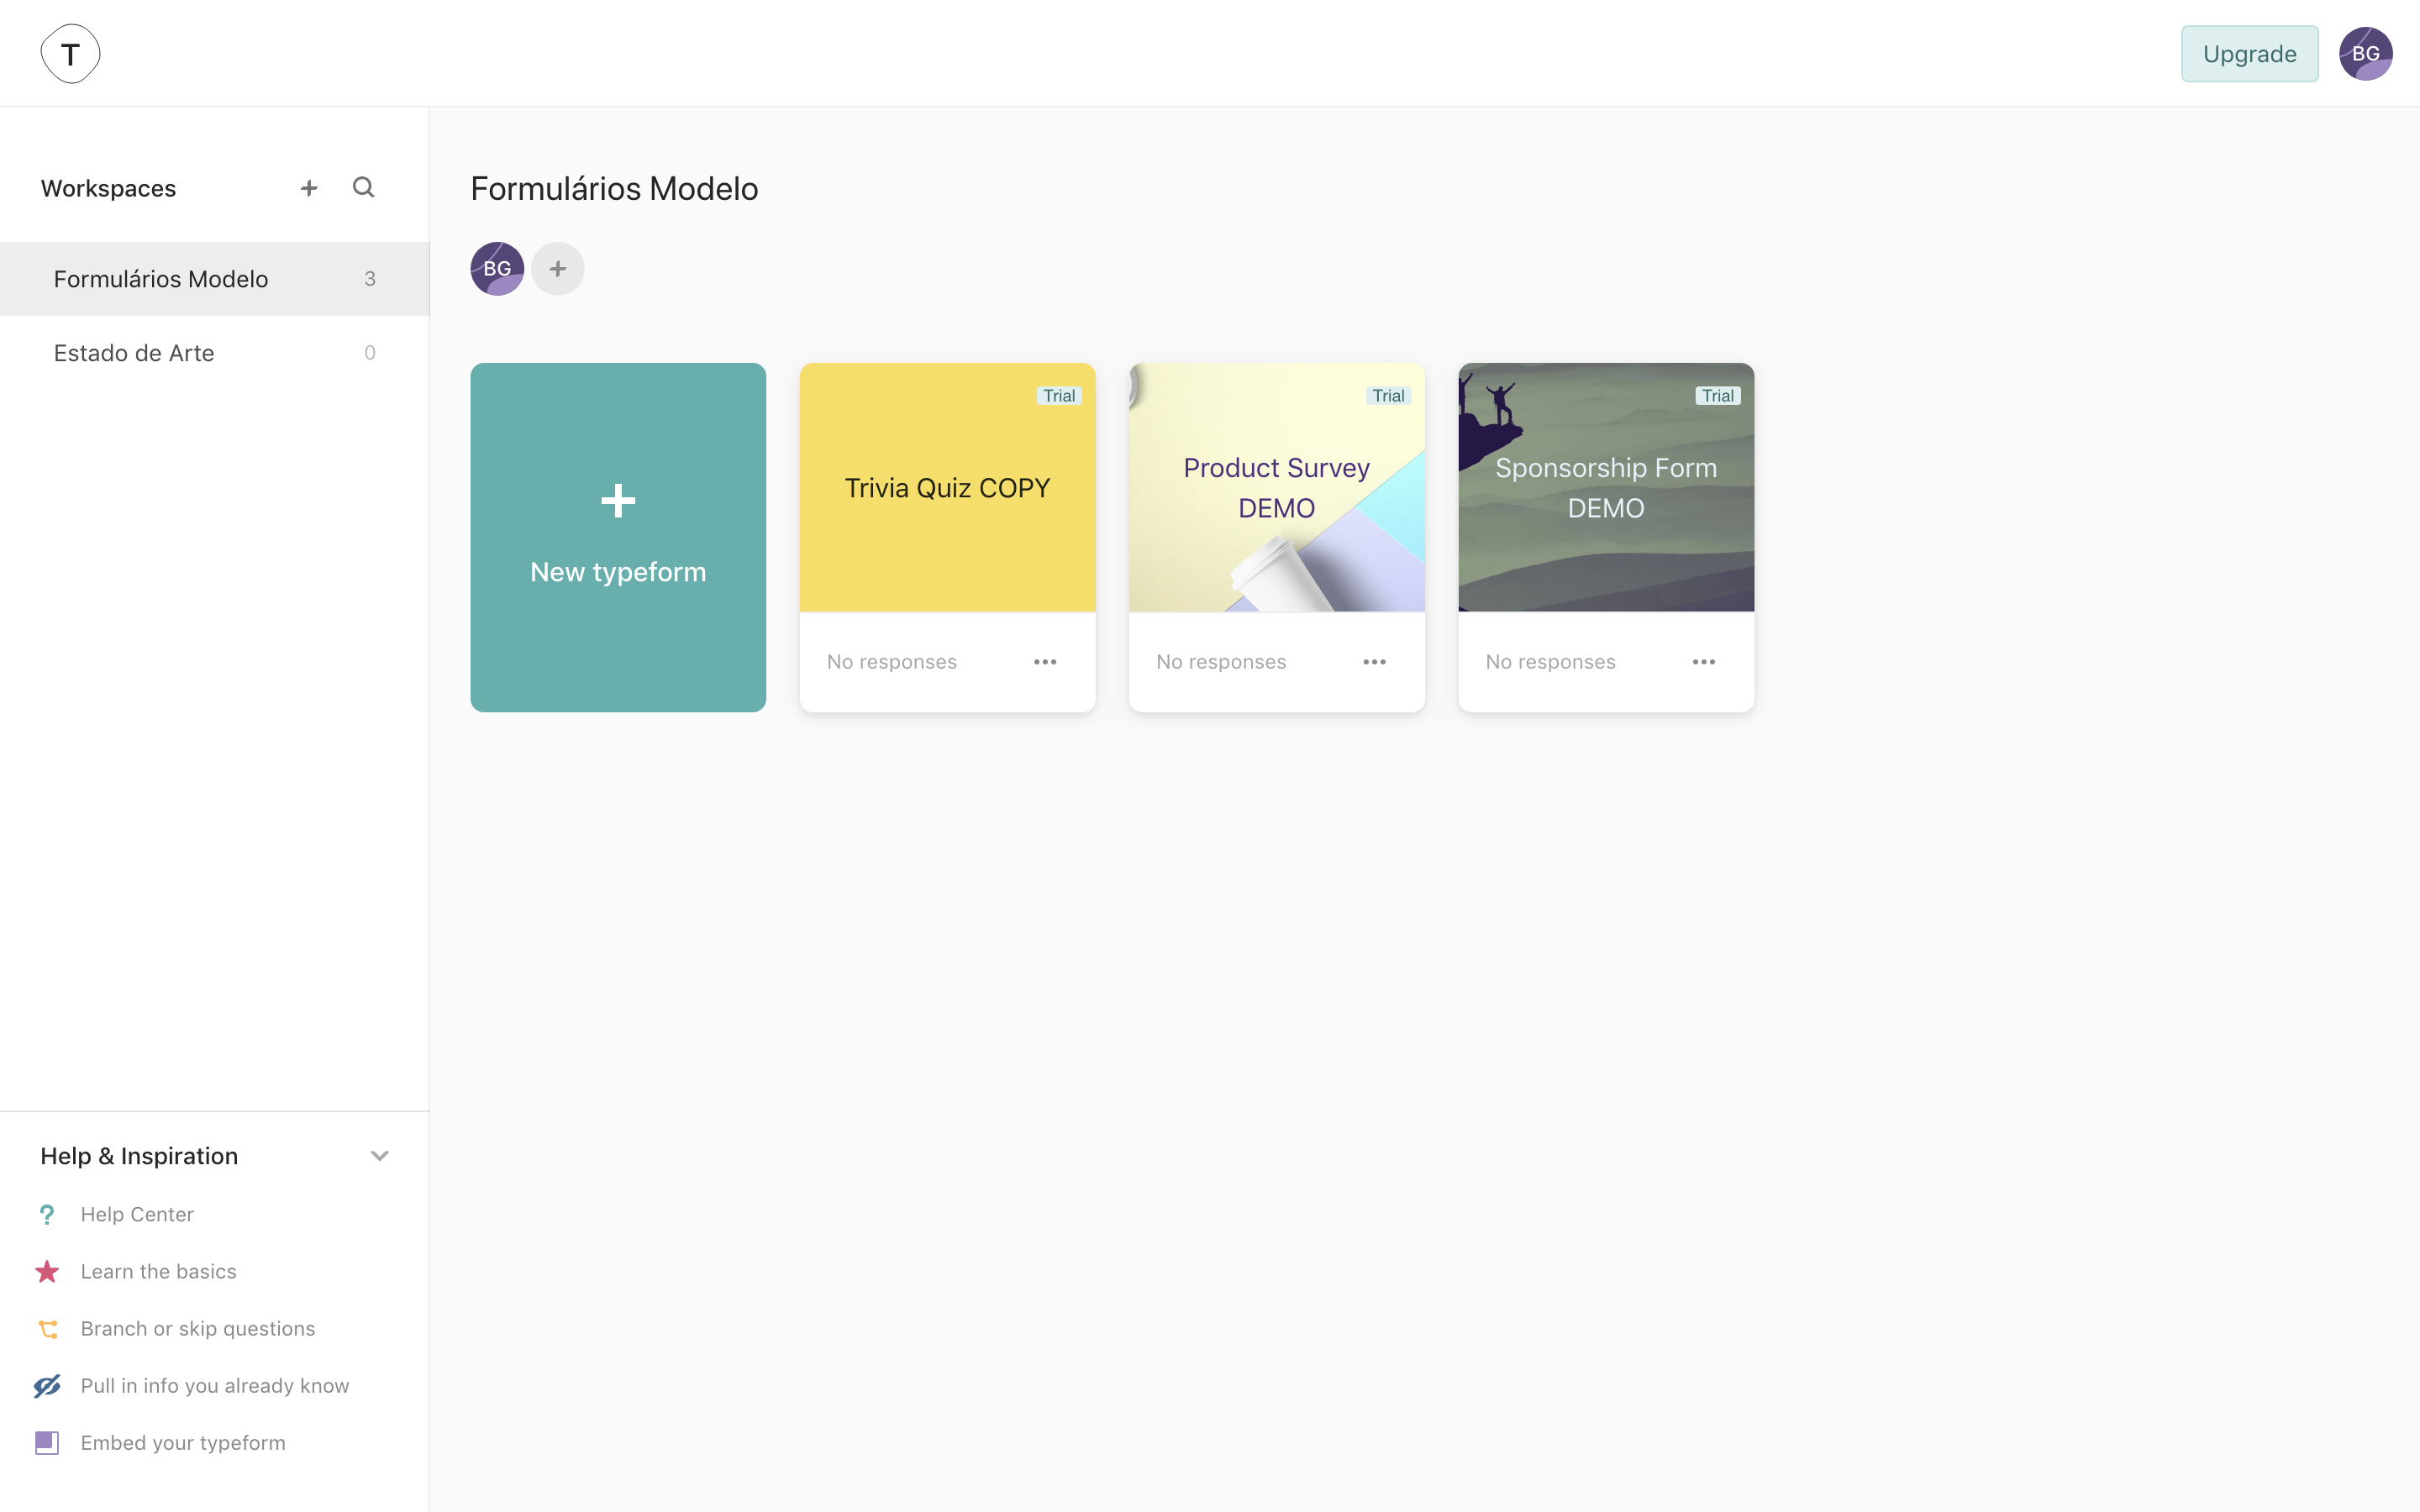
\includegraphics[width=1\textwidth]{img/tf/tf-dashboard}
		\caption{Typeform - Painel de Controlo}
		\label{fig:tf-dashboard}
	\end{center}
\end{figure}

Na criação de um formulário ou inquérito, do zero, a plataforma lista uma série de templates que se podem filtrar por categorias na coluna à esquerda, como se pode observar na Figura \ref{fig:tf-form-create}.

\begin{figure}[ht!]
	\begin{center}
		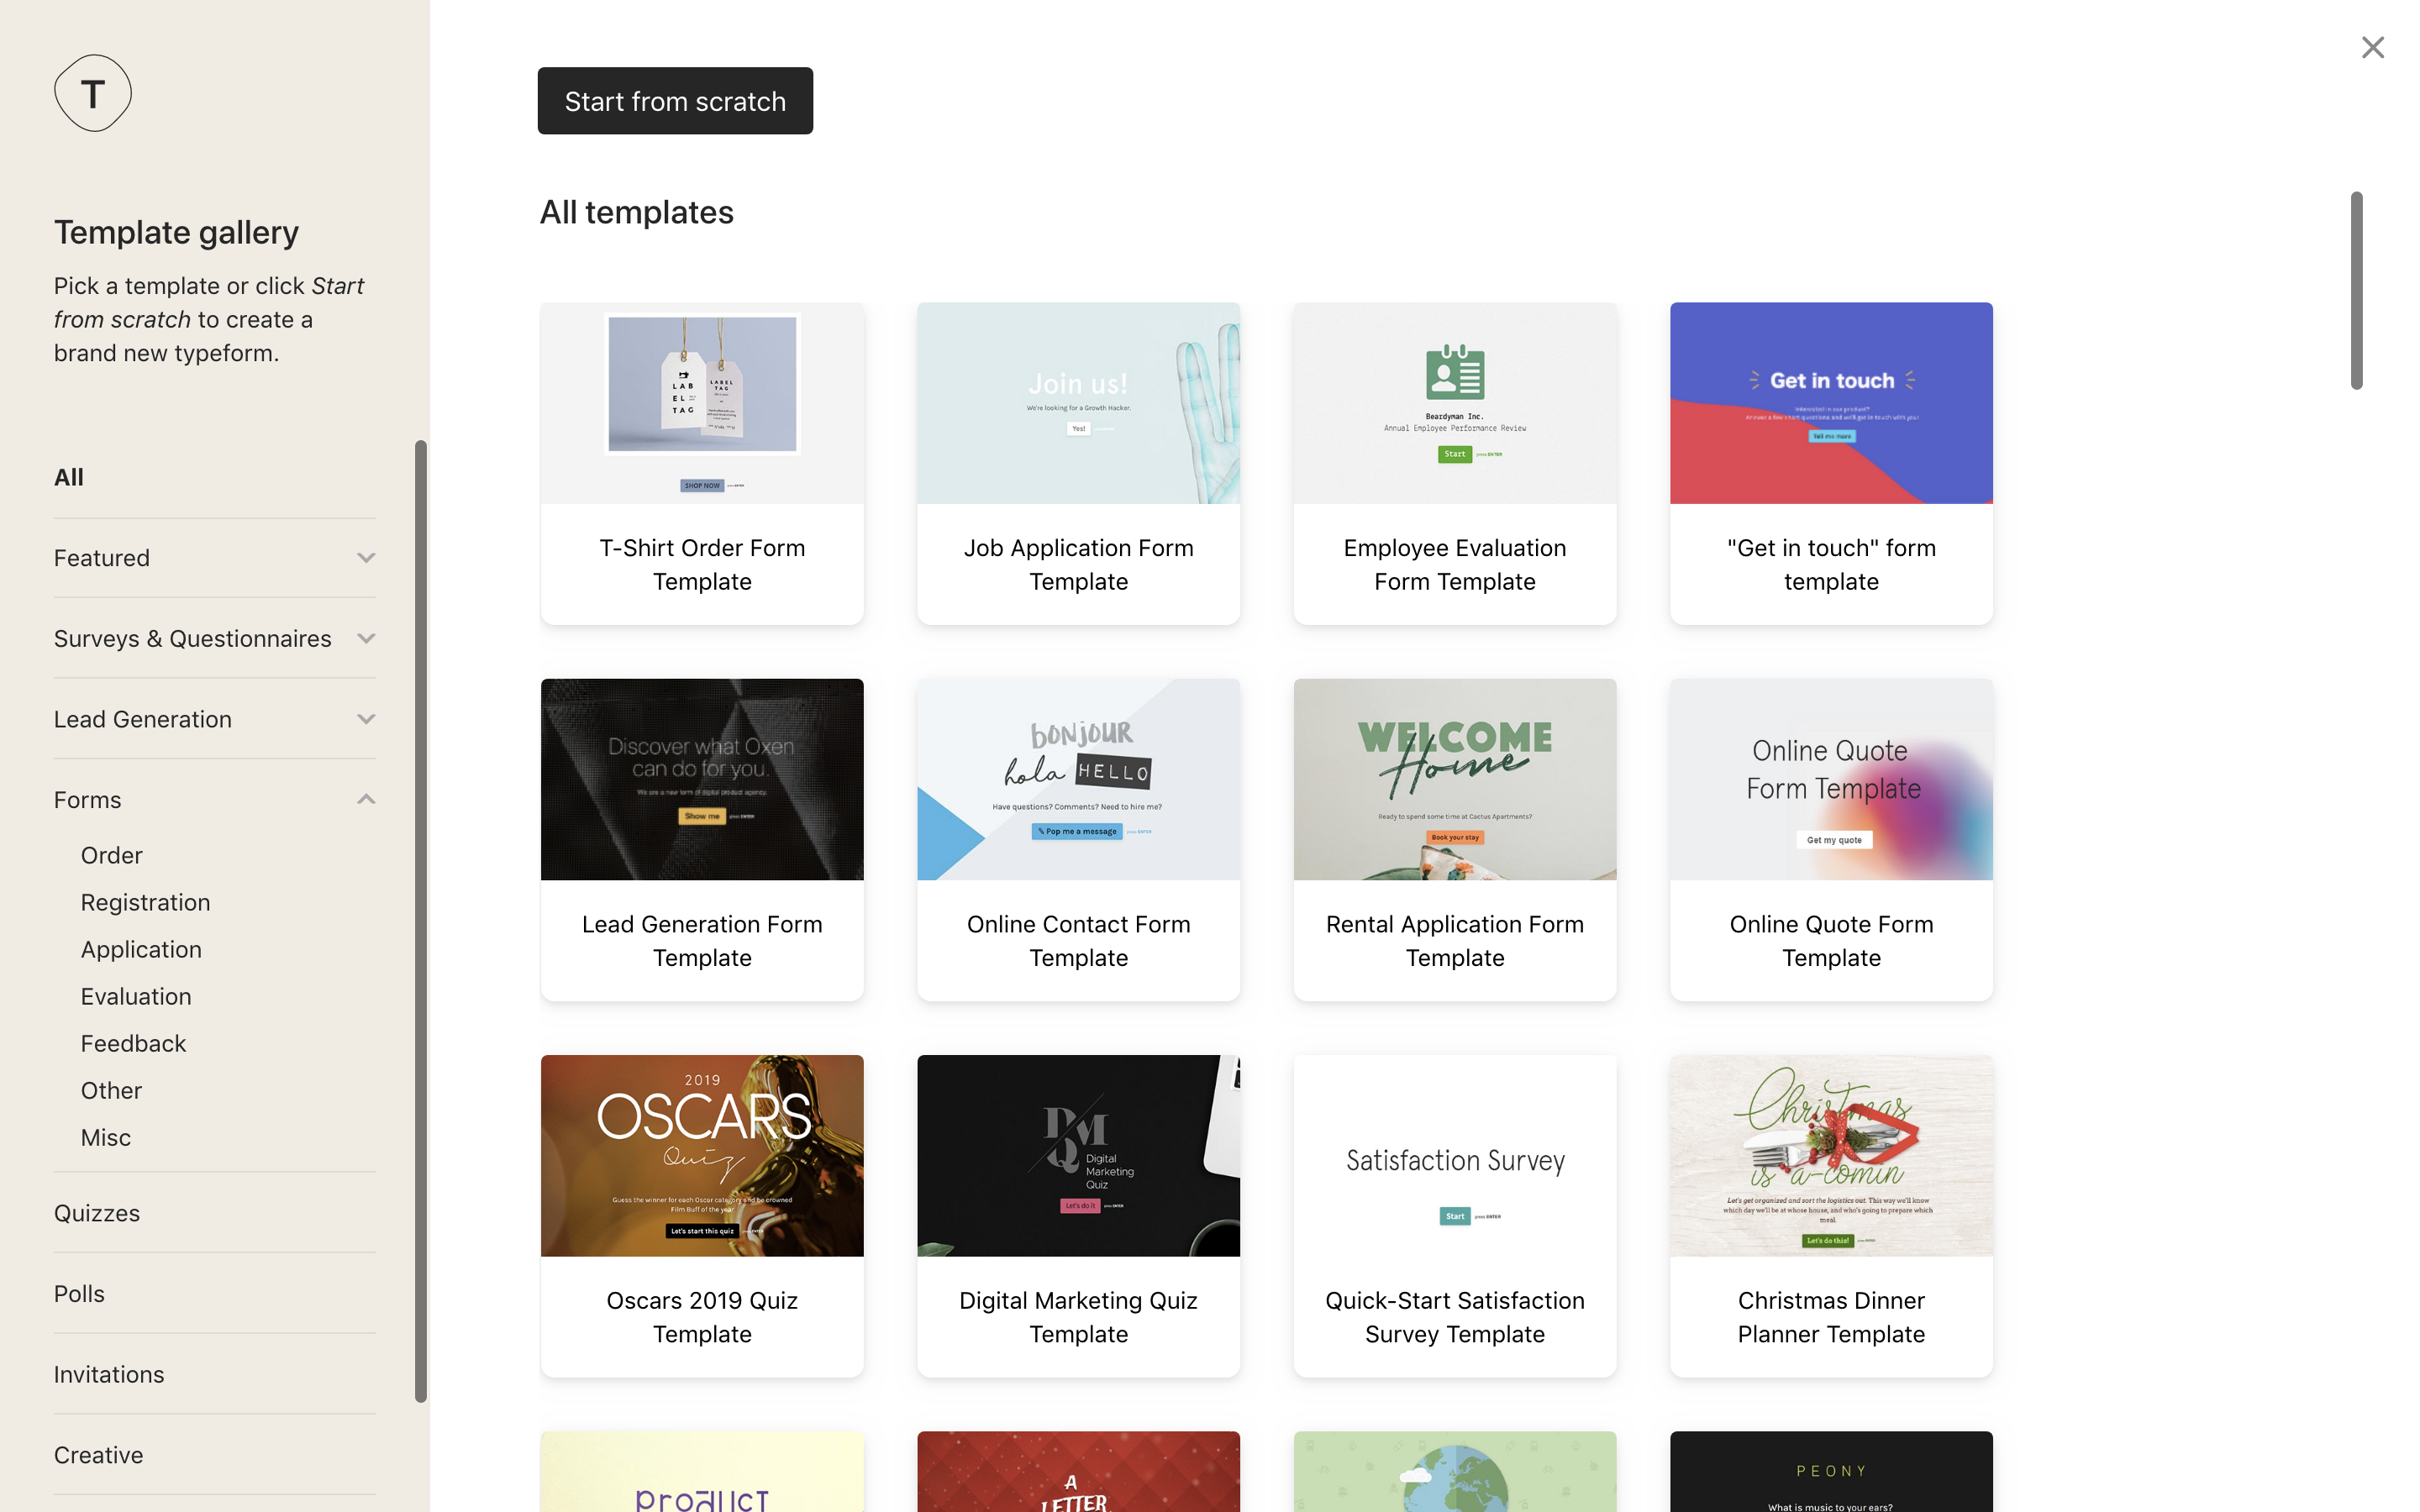
\includegraphics[width=1\textwidth]{img/tf/tf-form-create}
		\caption{Typeform - Criar Formulário}
		\label{fig:tf-form-create}
	\end{center}
\end{figure}
\newpage

\begin{figure}[ht!]
	\begin{center}
		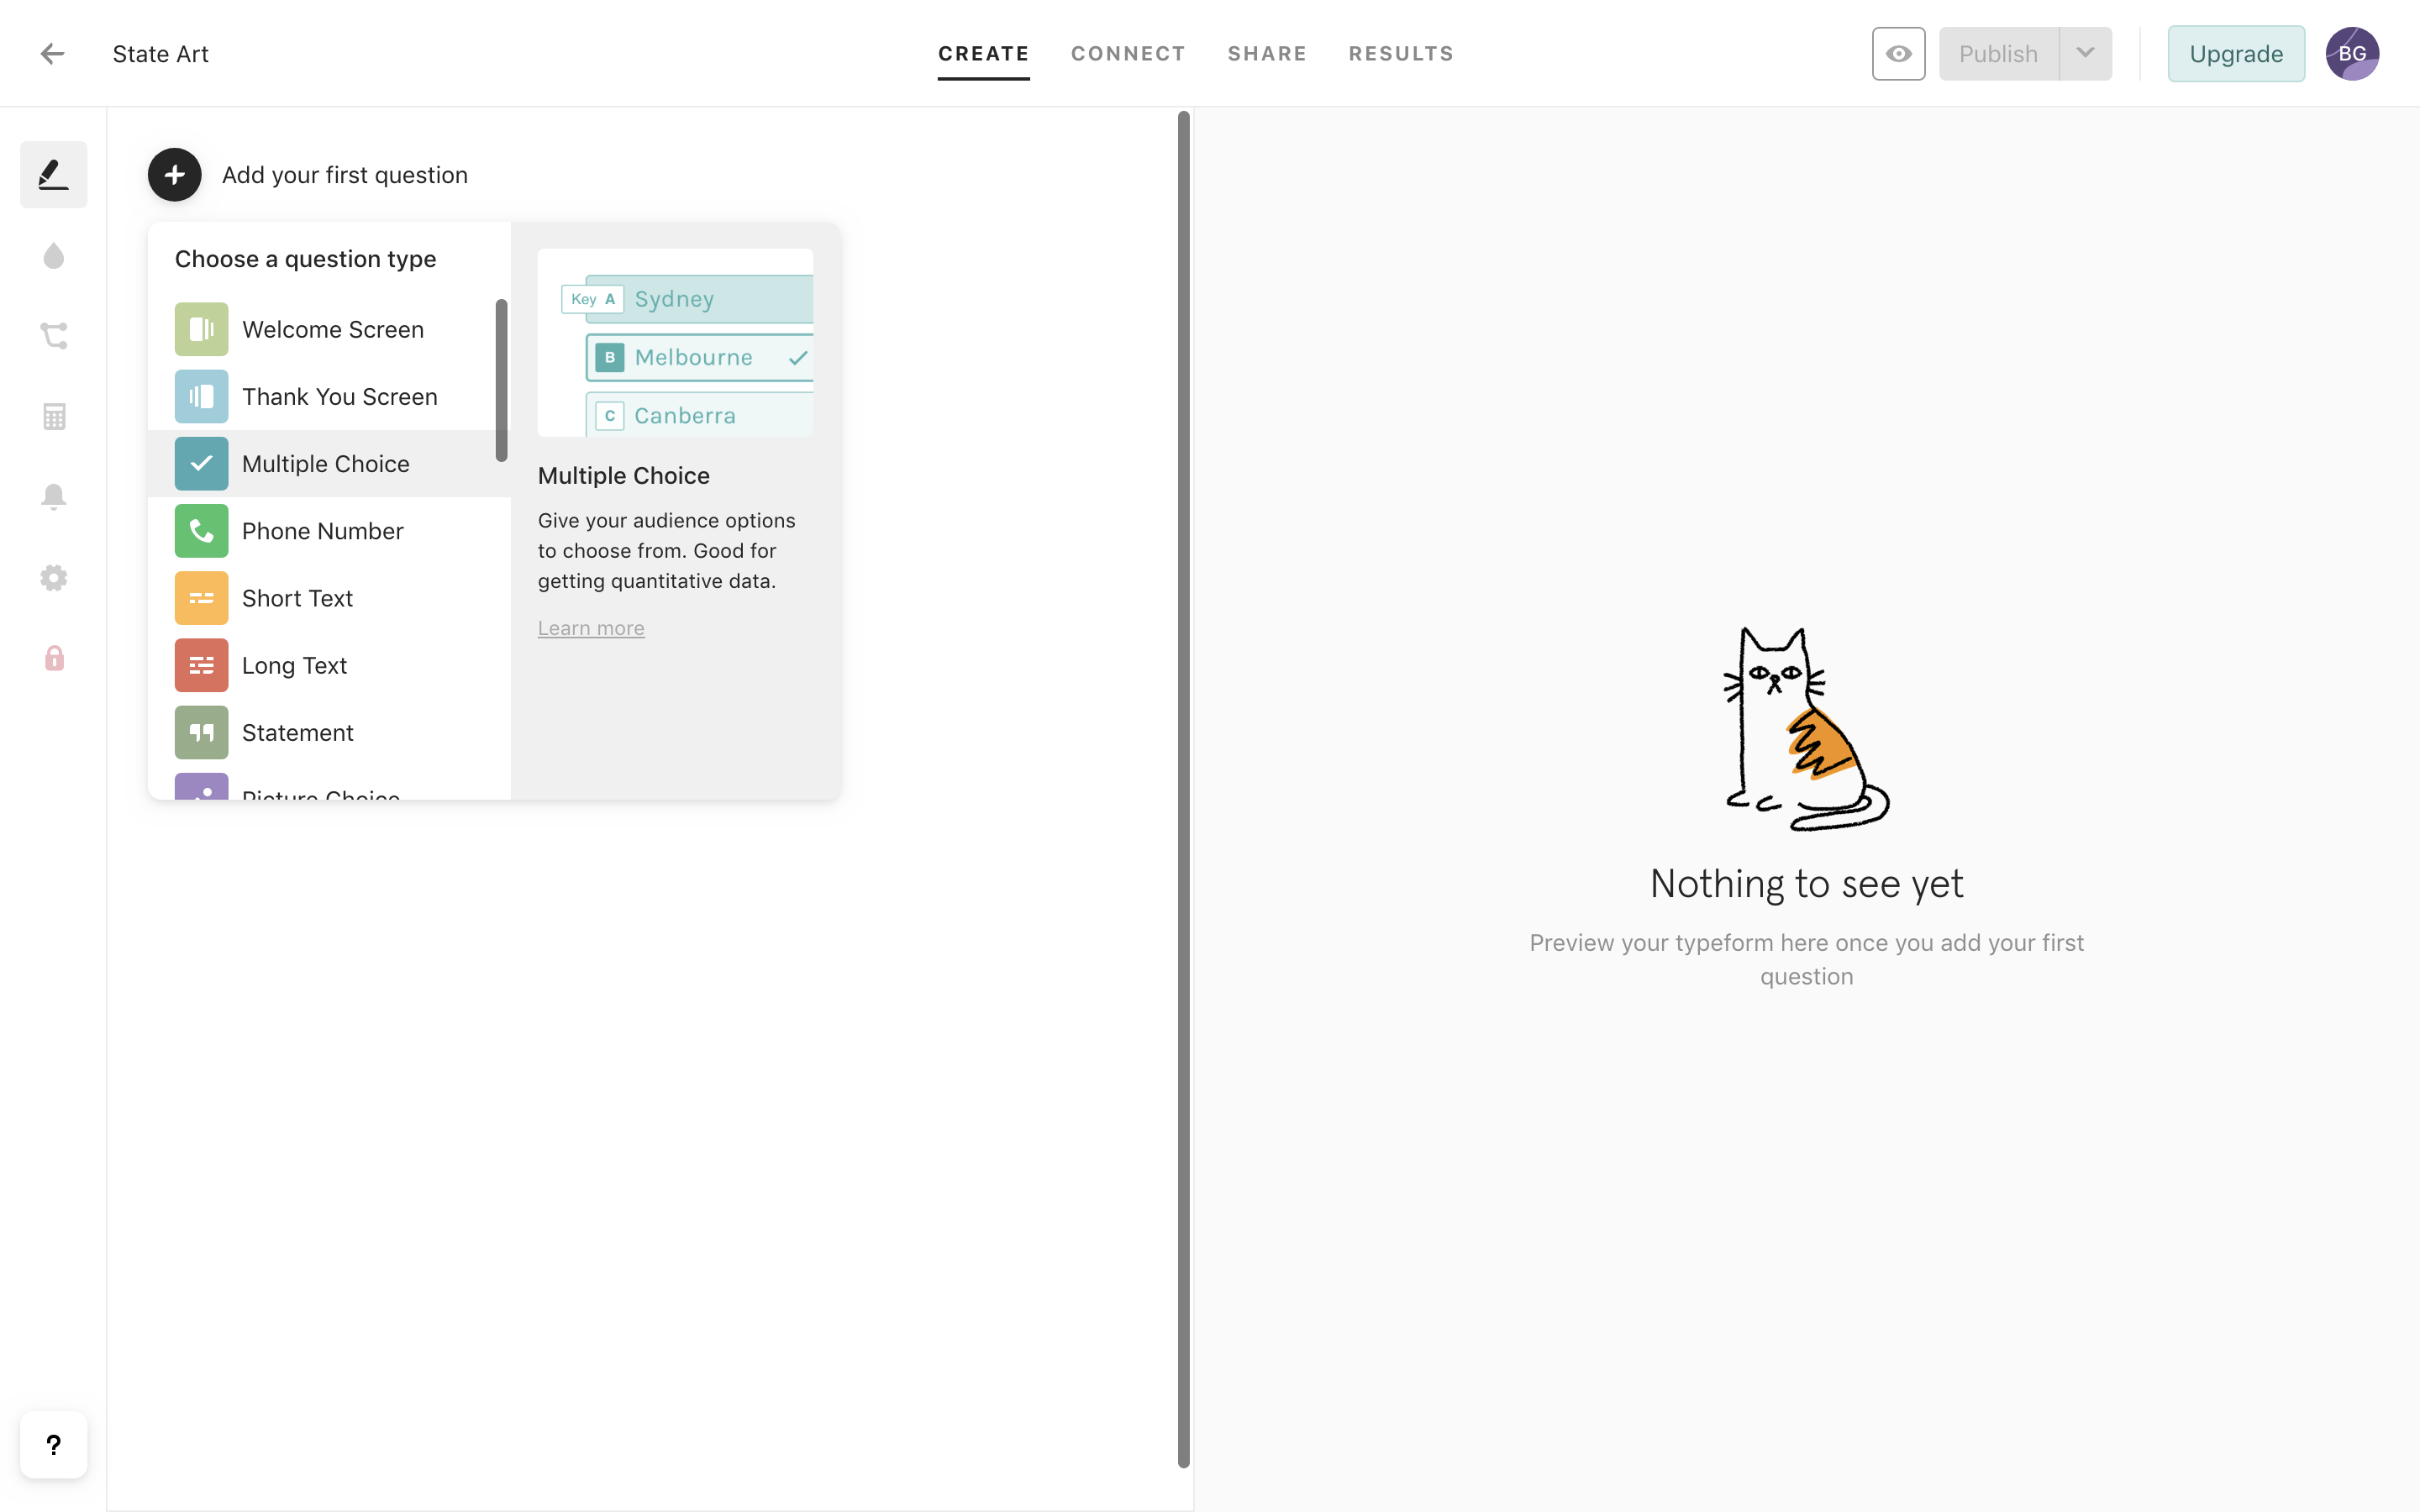
\includegraphics[width=1\textwidth]{img/tf/tf-question-type}
		\caption{Typeform - Tipos de pergunta}
		\label{fig:tf-question-type}
	\end{center}
\end{figure}

Representado na Figura \ref{fig:tf-question-type} temos os tipos de pergunta que a plataforma permite adicionar no formulário. Estas perguntas podem ser personalizadas tanto a nível estético como funcional como podemos ver nas Figuras \ref{fig:tf-question-opcoes} e \ref{fig:tf-question-custom}, respectivamente. É também possível criar um tema novo para cada pergunta onde se pode escolher a fonte de texto, imagem de fundo e cores da pergunta, respostas, botões e fundo.

\begin{figure}[ht!]
	\begin{center}
		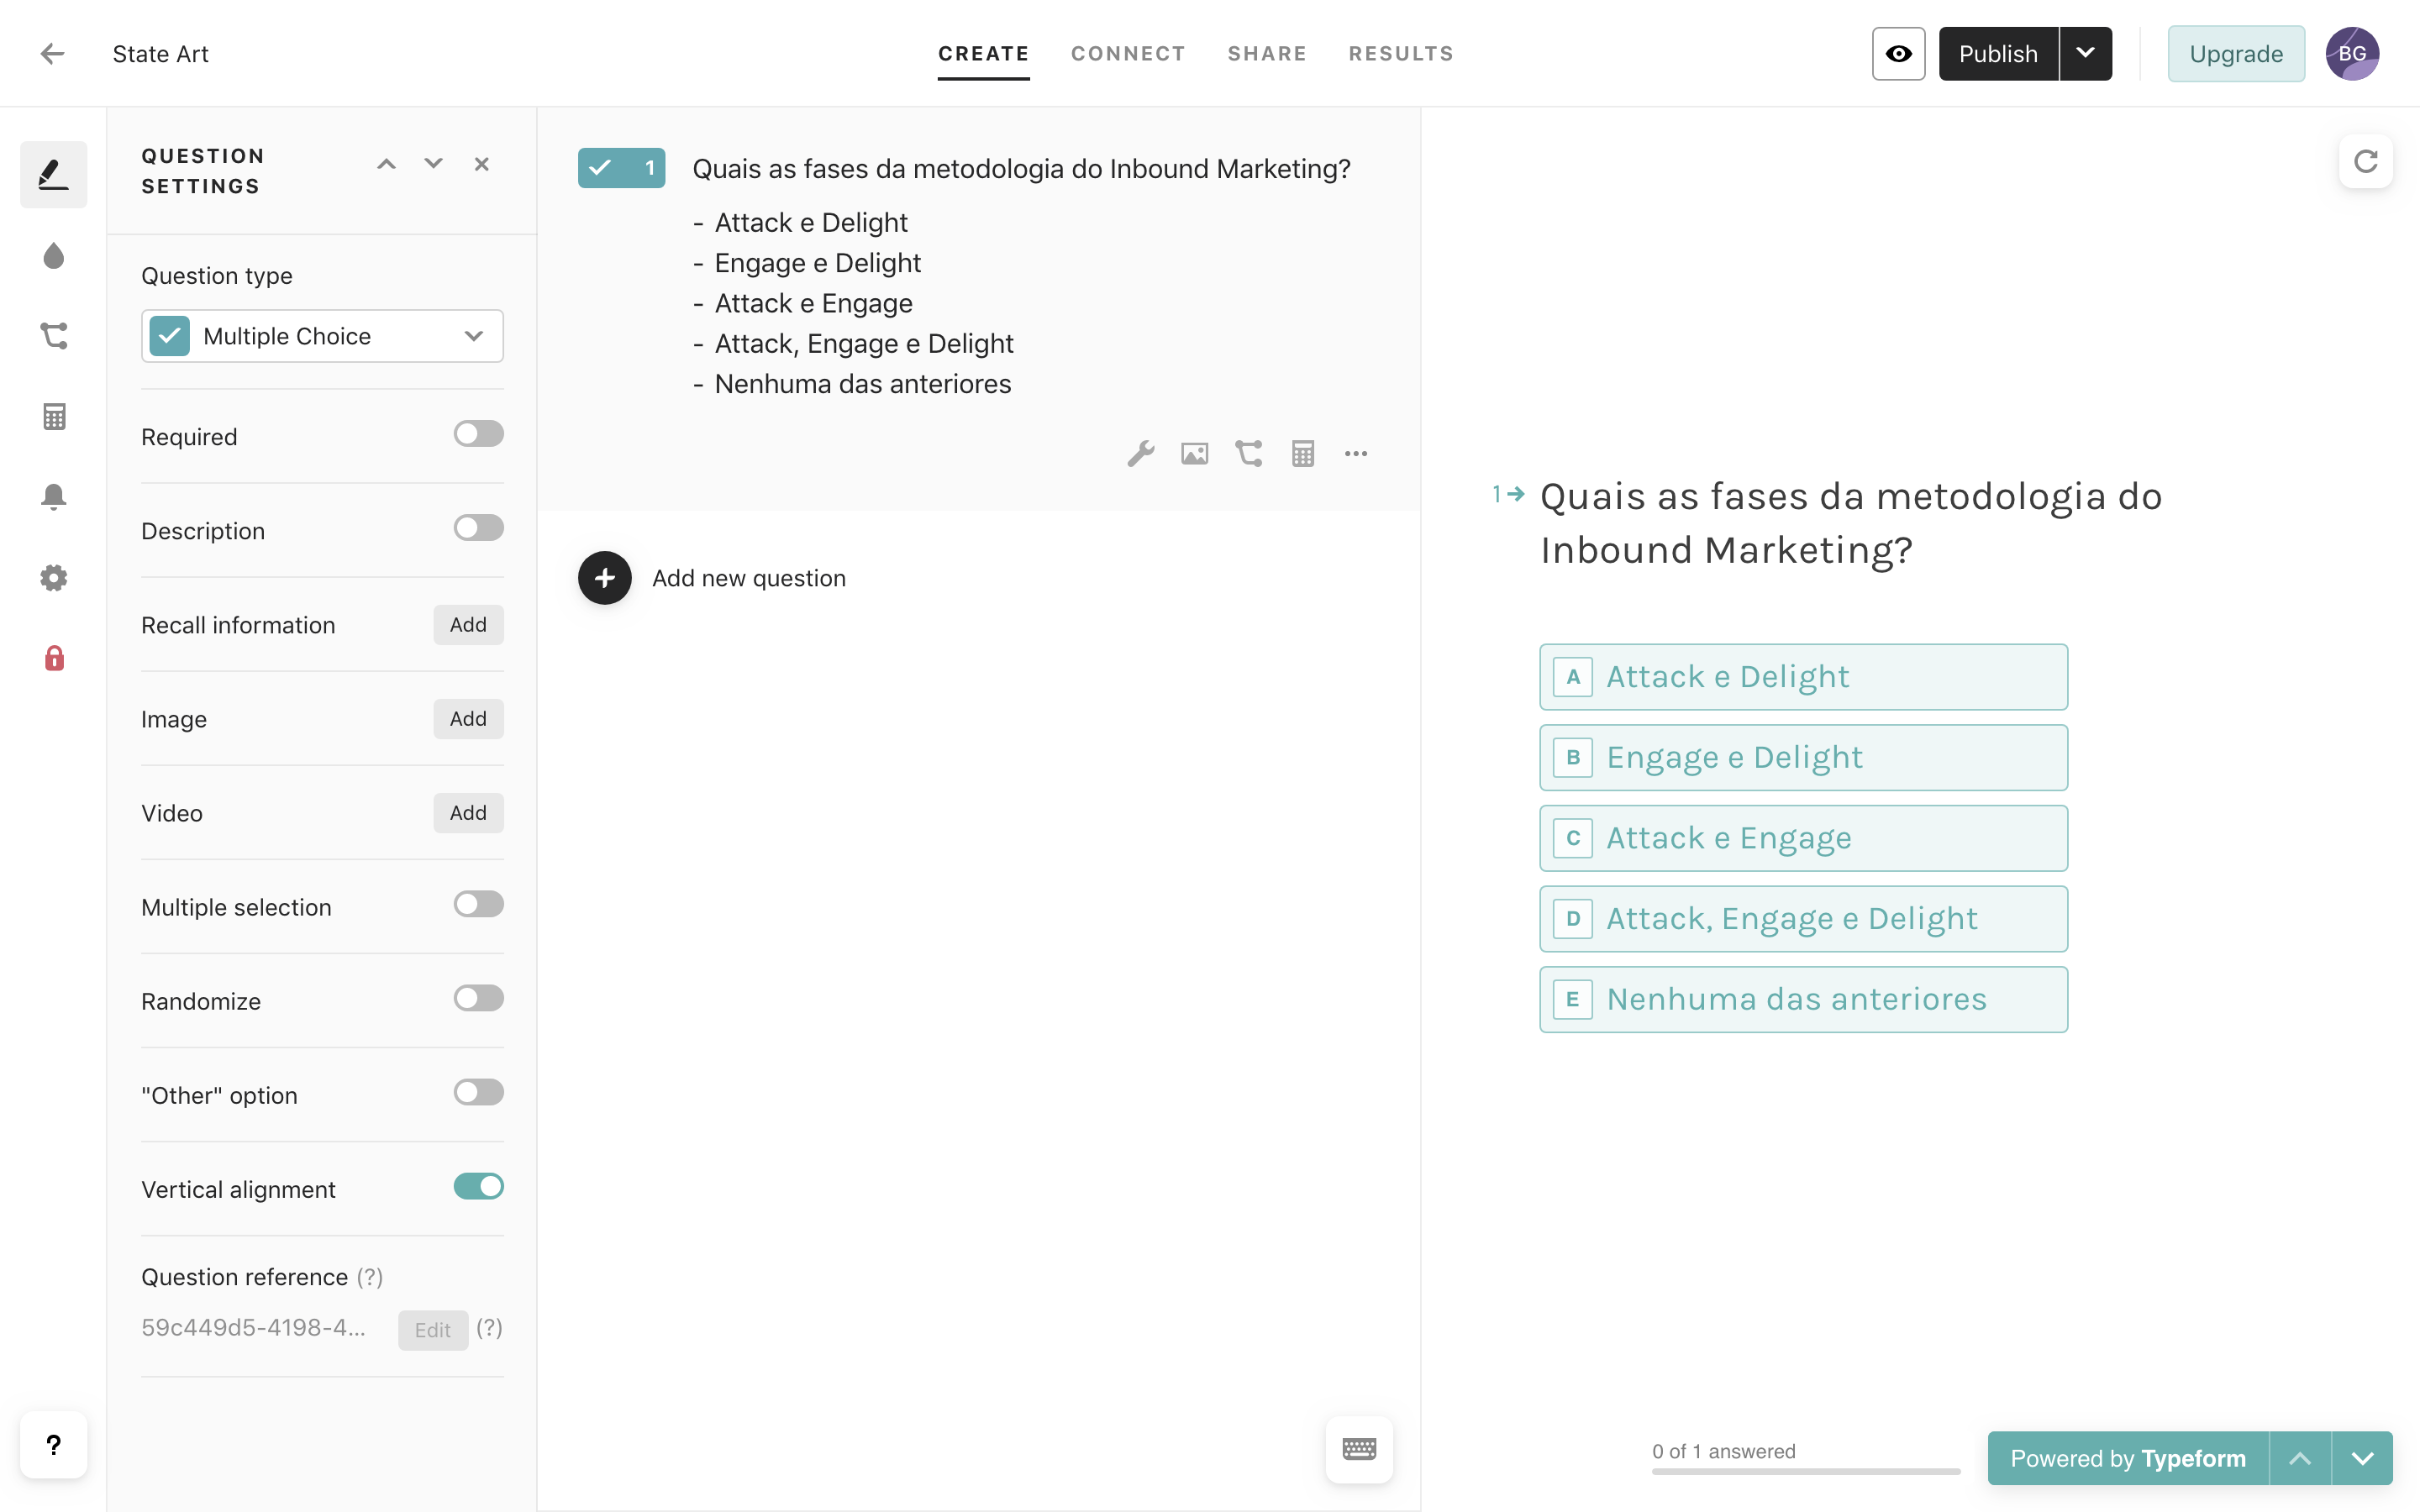
\includegraphics[width=1\textwidth]{img/tf/tf-question-opcoes}
		\caption{Typeform - Opções da pergunta}
		\label{fig:tf-question-opcoes}
	\end{center}
\end{figure}

\begin{figure}[ht!]
	\begin{center}
		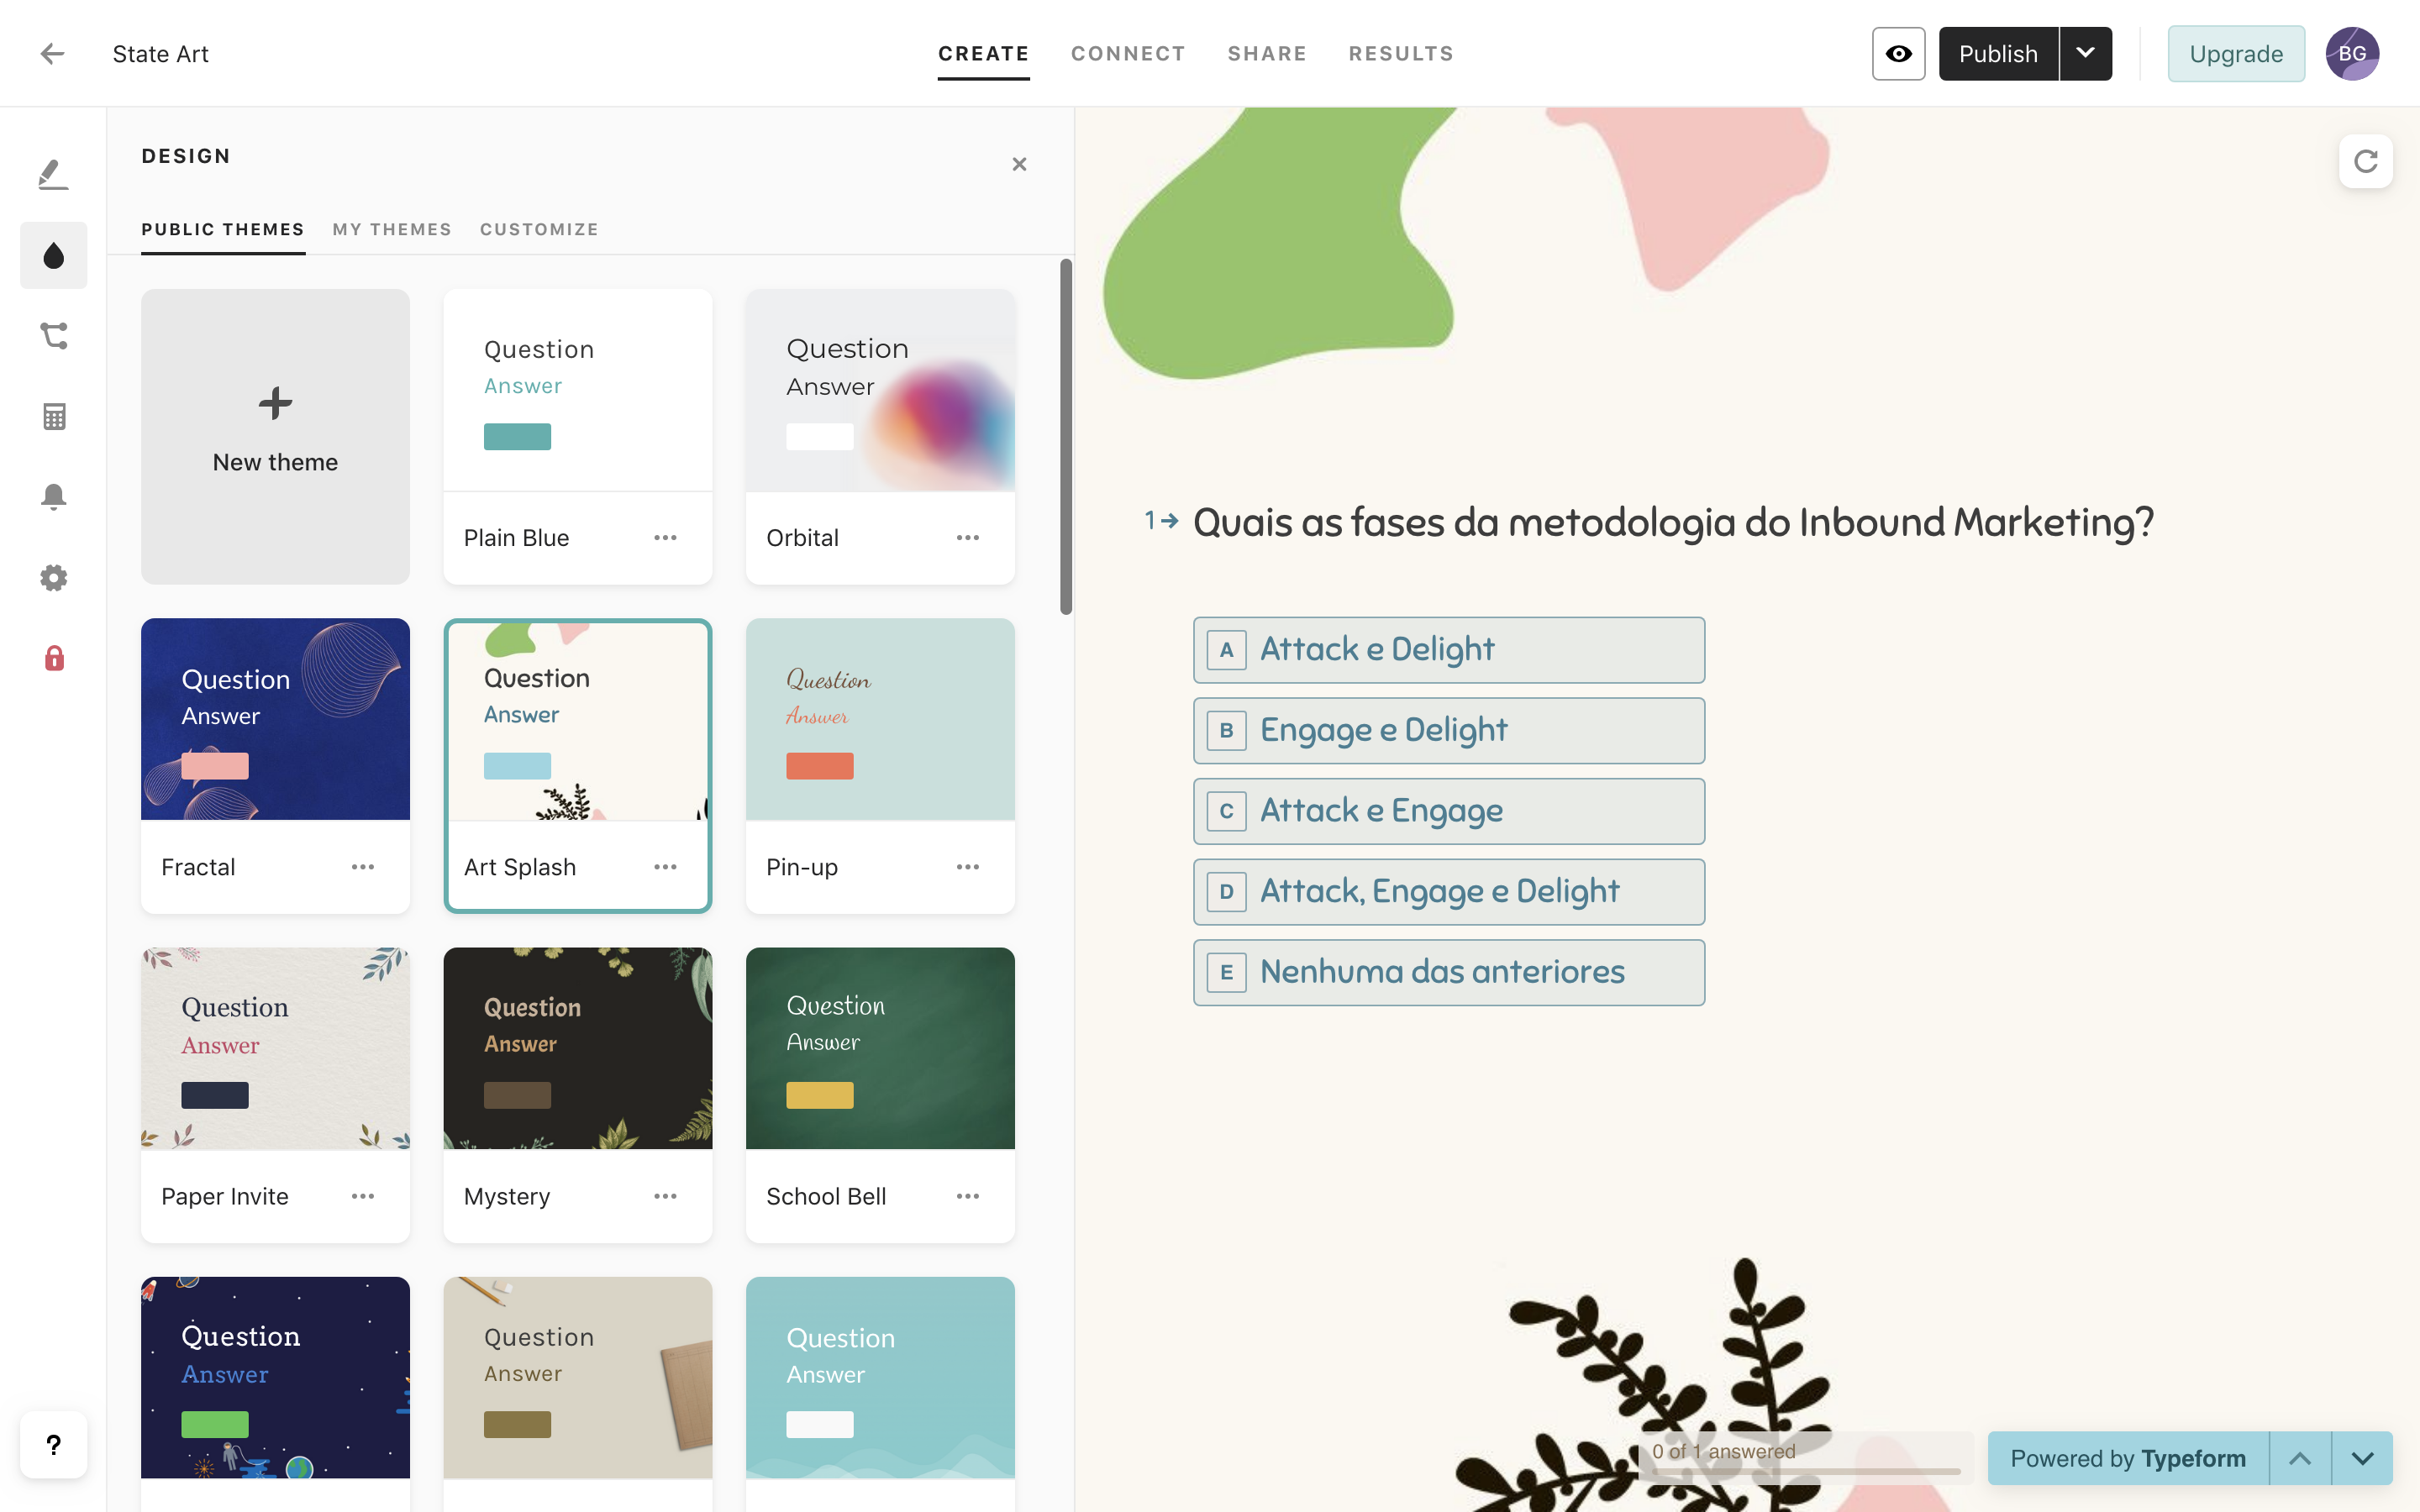
\includegraphics[width=1\textwidth]{img/tf/tf-question-custom}
		\caption{Typeform - Design da pergunta}
		\label{fig:tf-question-custom}
	\end{center}
\end{figure}

A plataforma permite ainda os utilizadores adicionarem lógicas aos seus formulário, como exemplificado na Figura \ref{fig:tf-question-logica} , em que caso a resposta à pergunta 4 seja a especificada, o caminho a tomar será diferente. 



\begin{figure}[ht!]
	\begin{center}
		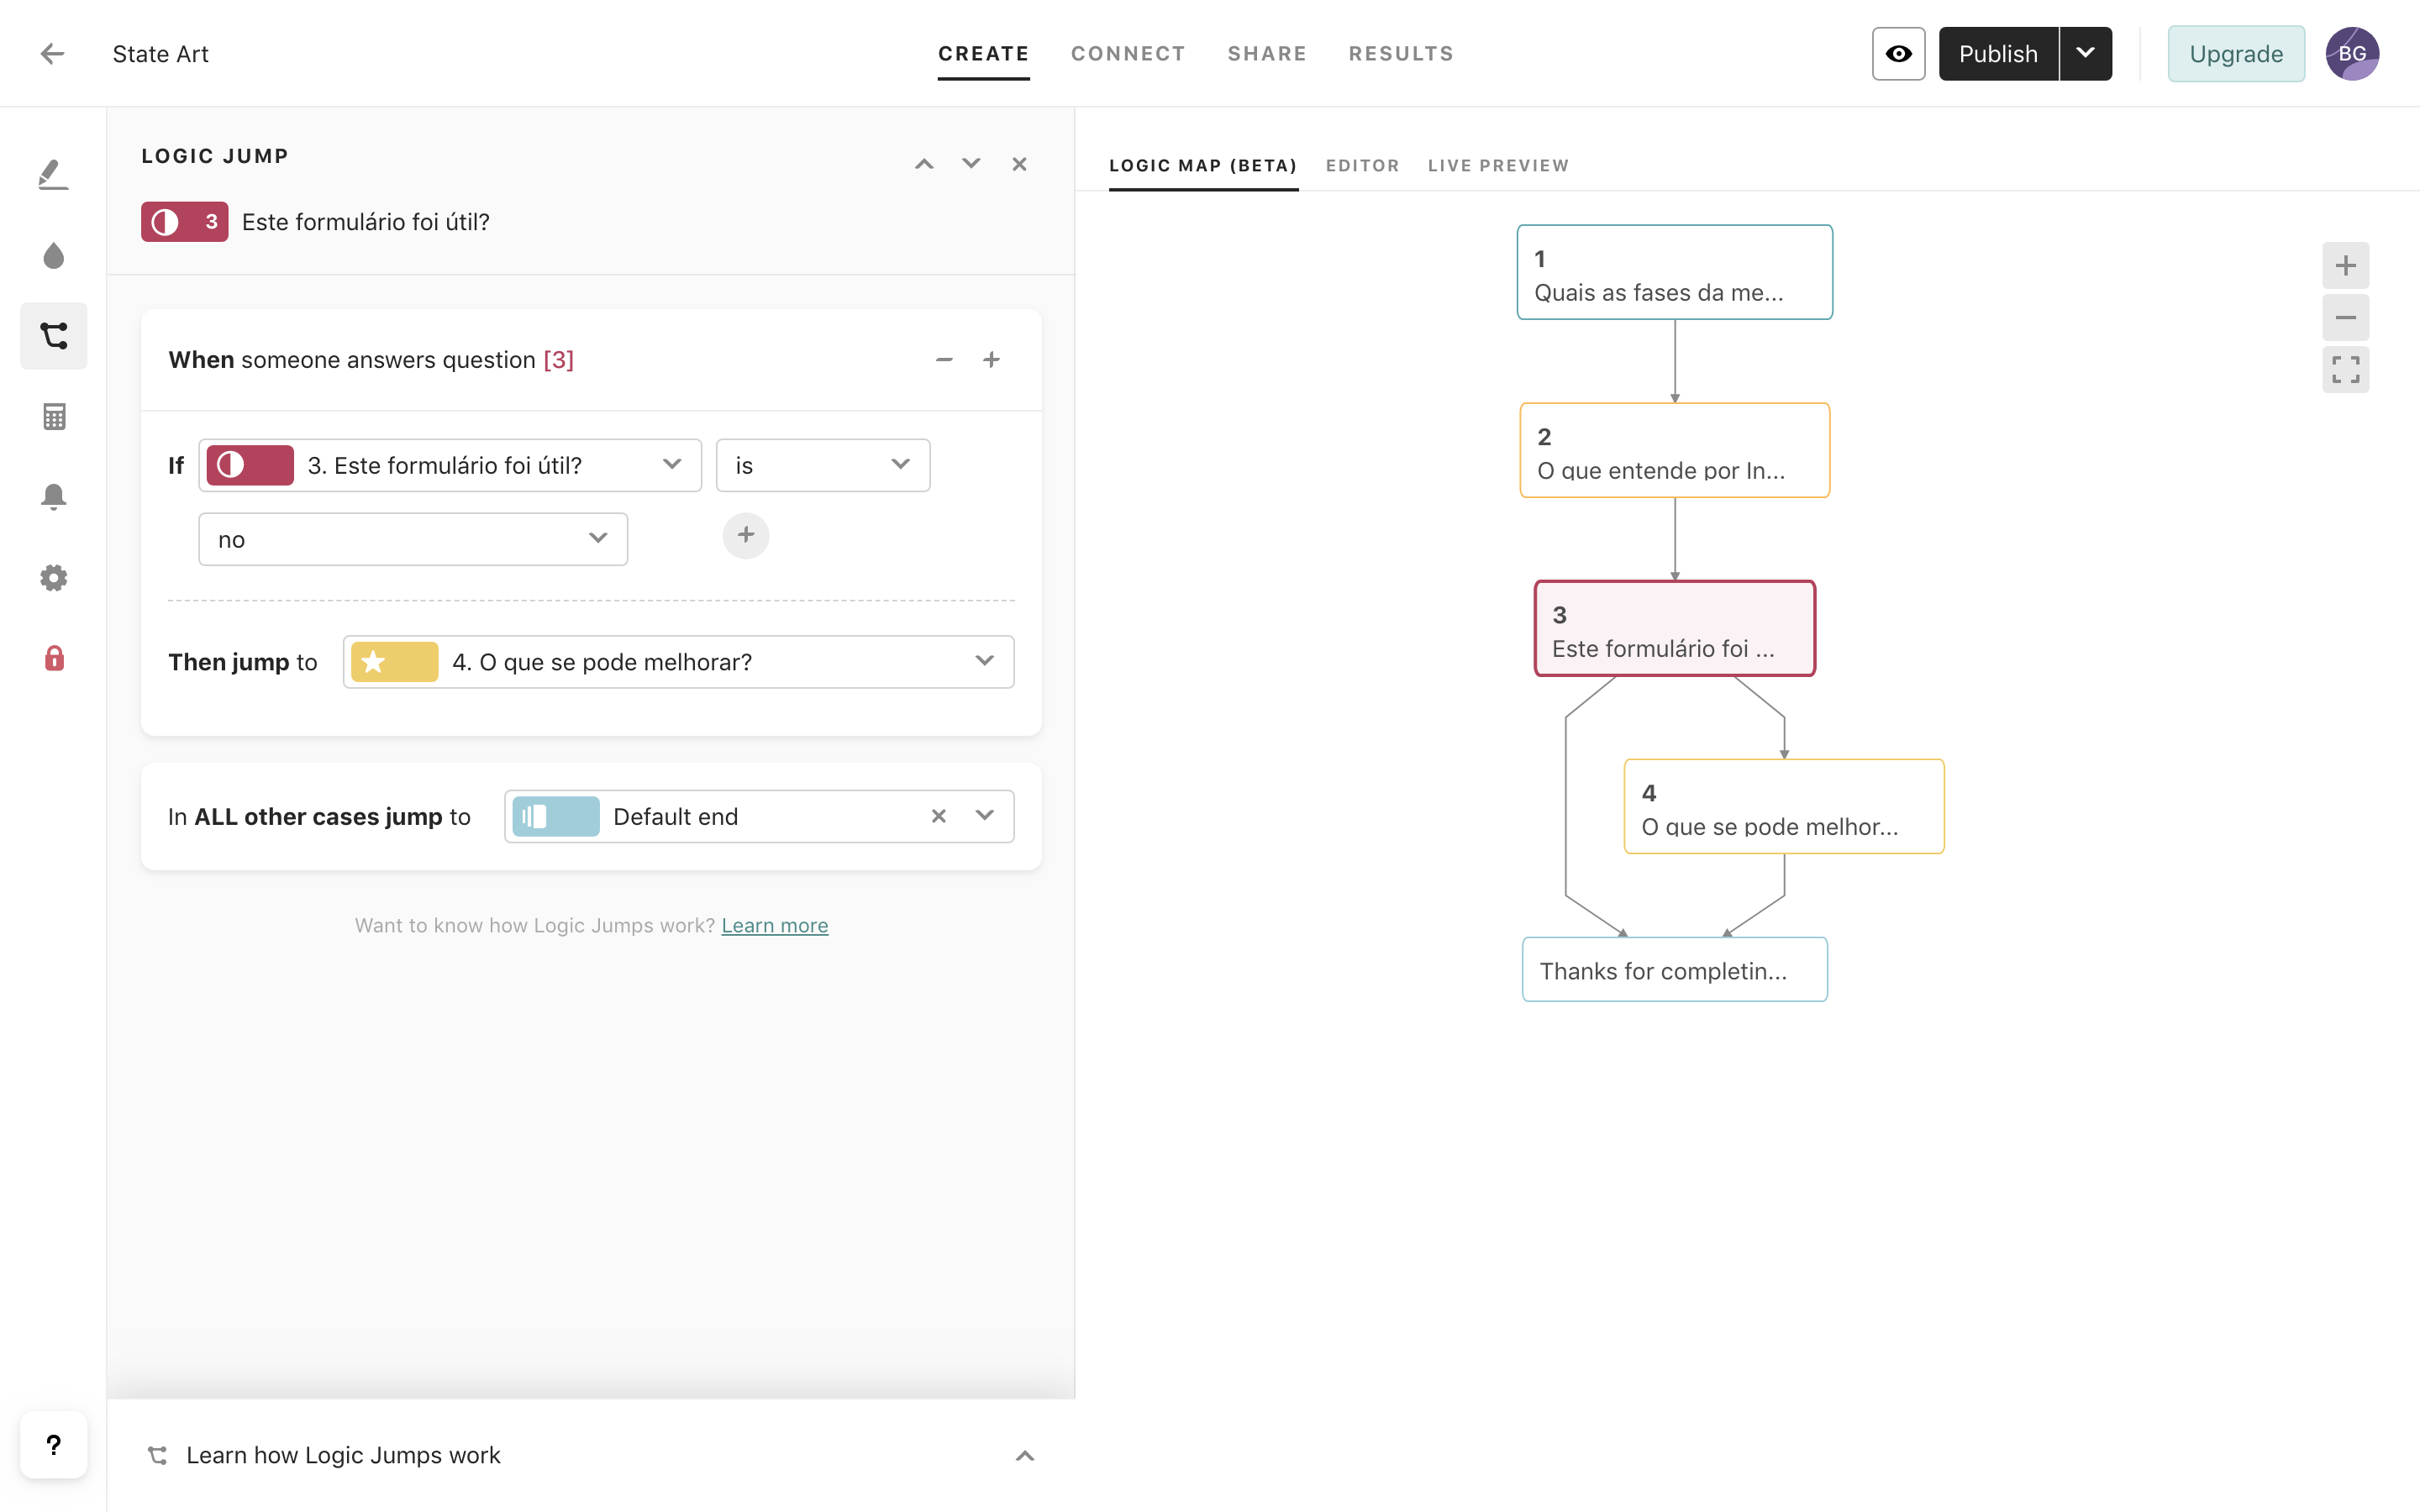
\includegraphics[width=1\textwidth]{img/tf/tf-question-logica}
		\caption{Typeform - Lógica do formulário}
		\label{fig:tf-question-logica}
	\end{center}
\end{figure}

\newpage

A funcionalidade de visualizar o formulário está disponível no canto superior direito, no lado esquerdo do botão de publicar, que permite o autor verificar se tudo está feito conforme planeado e assim poder publicar e partilhar.

O Typeform permite também a integração de serviços externos com o formulário, como podemos ver na Figura \ref{fig:tf-question-integration} , em que, por exemplo, utilizando o Google Sheets\cite{googlesheets}, os resultados são exportados diretamente para uma \textit{google sheet}


\begin{figure}[ht!]
	\begin{center}
		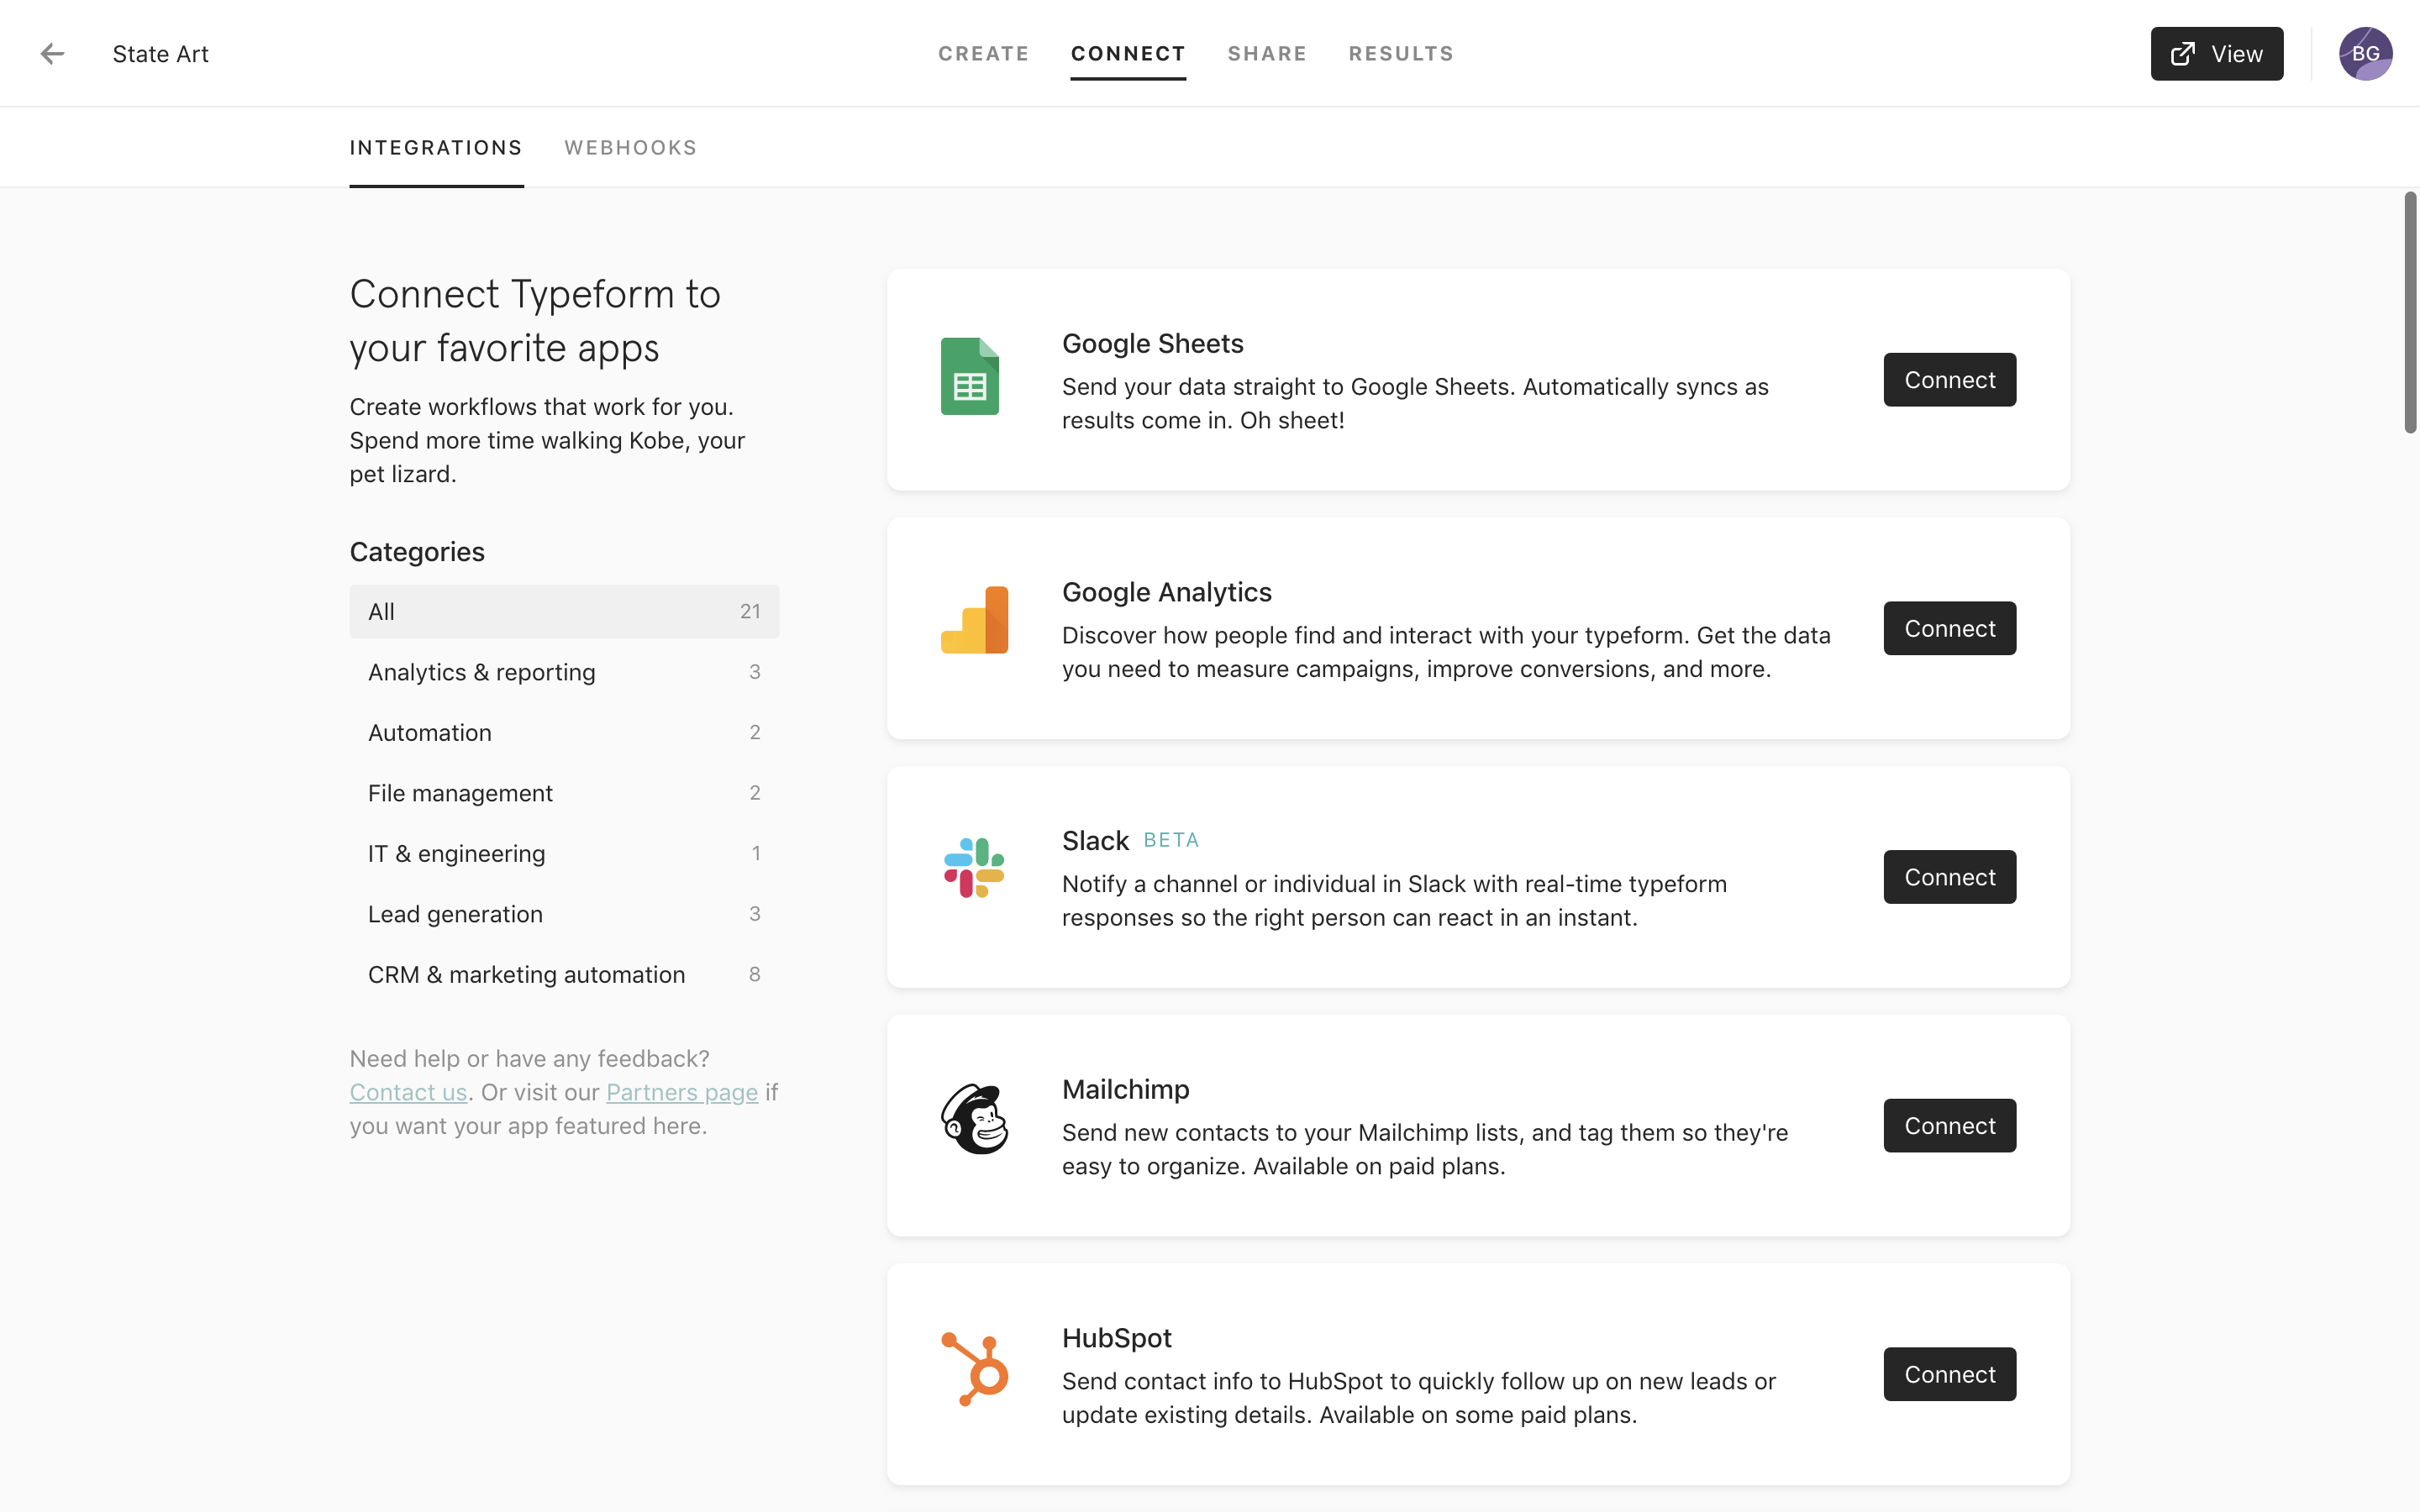
\includegraphics[width=1\textwidth]{img/tf/tf-question-integration}
		\caption{Typeform - Integração com sistemas externos}
		\label{fig:tf-question-integration}
	\end{center}
\end{figure}

Representado na Figura \ref{fig:tf-question-results} , temos a secção de análise de dados da plataforma onde podemos ver uma sumarização dos dados recebidos ou  analisar todas as respostas uma a uma. É também possível gerar um reportório dos dados recebidos e partilhar com alguém em qualquer fase, por exemplo, de uma campanha, uma vez que o mesmo é actualizado automaticamente com as novas respostas recebidas. 

O Typeform não fornece quaisquer filtros para segmentar os dados, contudo, fora as respostas em si, exibe algumas estatísticas/métricas relacionadas com os dispositivos que foram utilizados para responder aos formulários.


\newpage
\begin{figure}[ht!]
	\begin{center}
		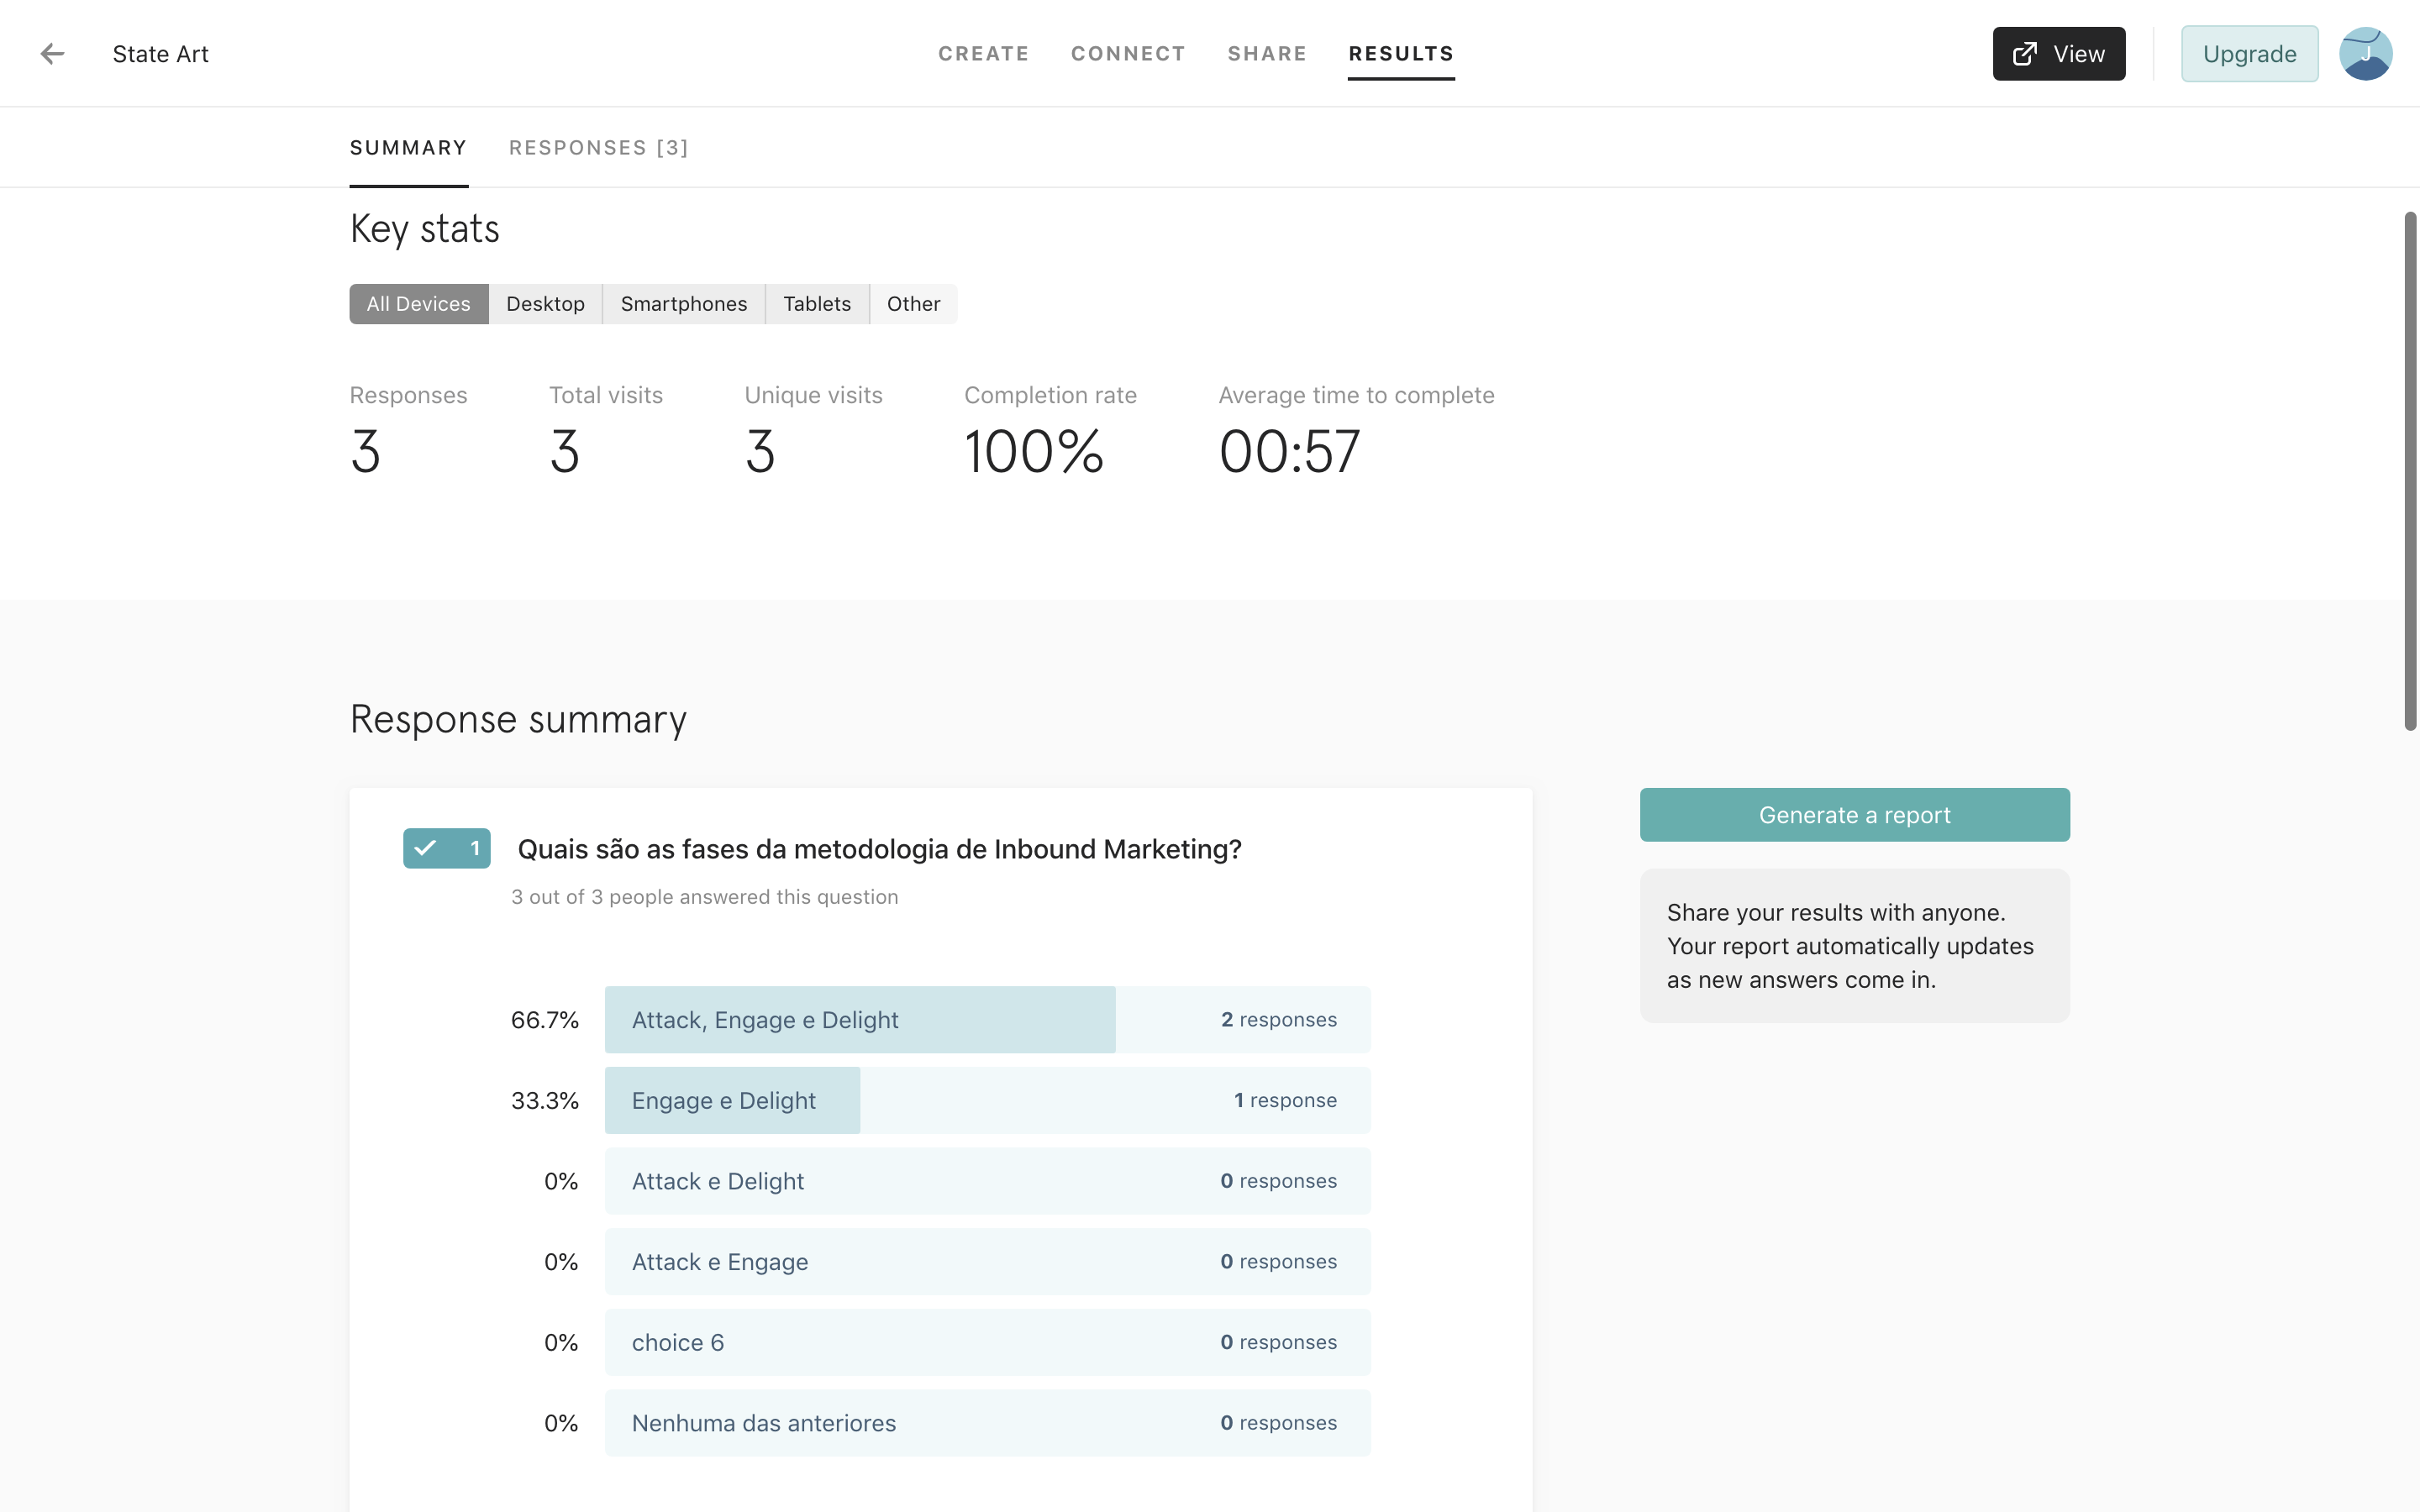
\includegraphics[width=1\textwidth]{img/tf/tf-question-results}
		\caption{Typeform - Análise de resultados}
		\label{fig:tf-question-results}
	\end{center}
\end{figure}

\section{Google Form}
\label{googleform}

O Google Form é uma aplicação de administração de inquéritos que está incluída no Google Drive office juntamente com o Google Docs\cite{gdocs}, Google Sheets e Google Slides\cite{gslides}. Esta ferramenta permite recolher informações do público alvo através de formulários e inquéritos personalizados e automaticamente exportar os dados para uma \textit{google sheet}.

Esta aplicação é totalmente gratuita, bastando  apenas criar uma conta Google para poder aceder a todas as funcionalidades da ferramenta.

Representado na Figura \ref{fig:gf-dashboard}, está o painel de controlo da conta de um utilizador, onde o mesmo pode visualizar os formulários com que interagiu recentemente. Por cima dos formulários recentes temos o botão para criar um novo formulário juntamente com alguns \textit{templates}/recomendações de formulários.

\newpage

\begin{figure}[ht!]
	\begin{center}
		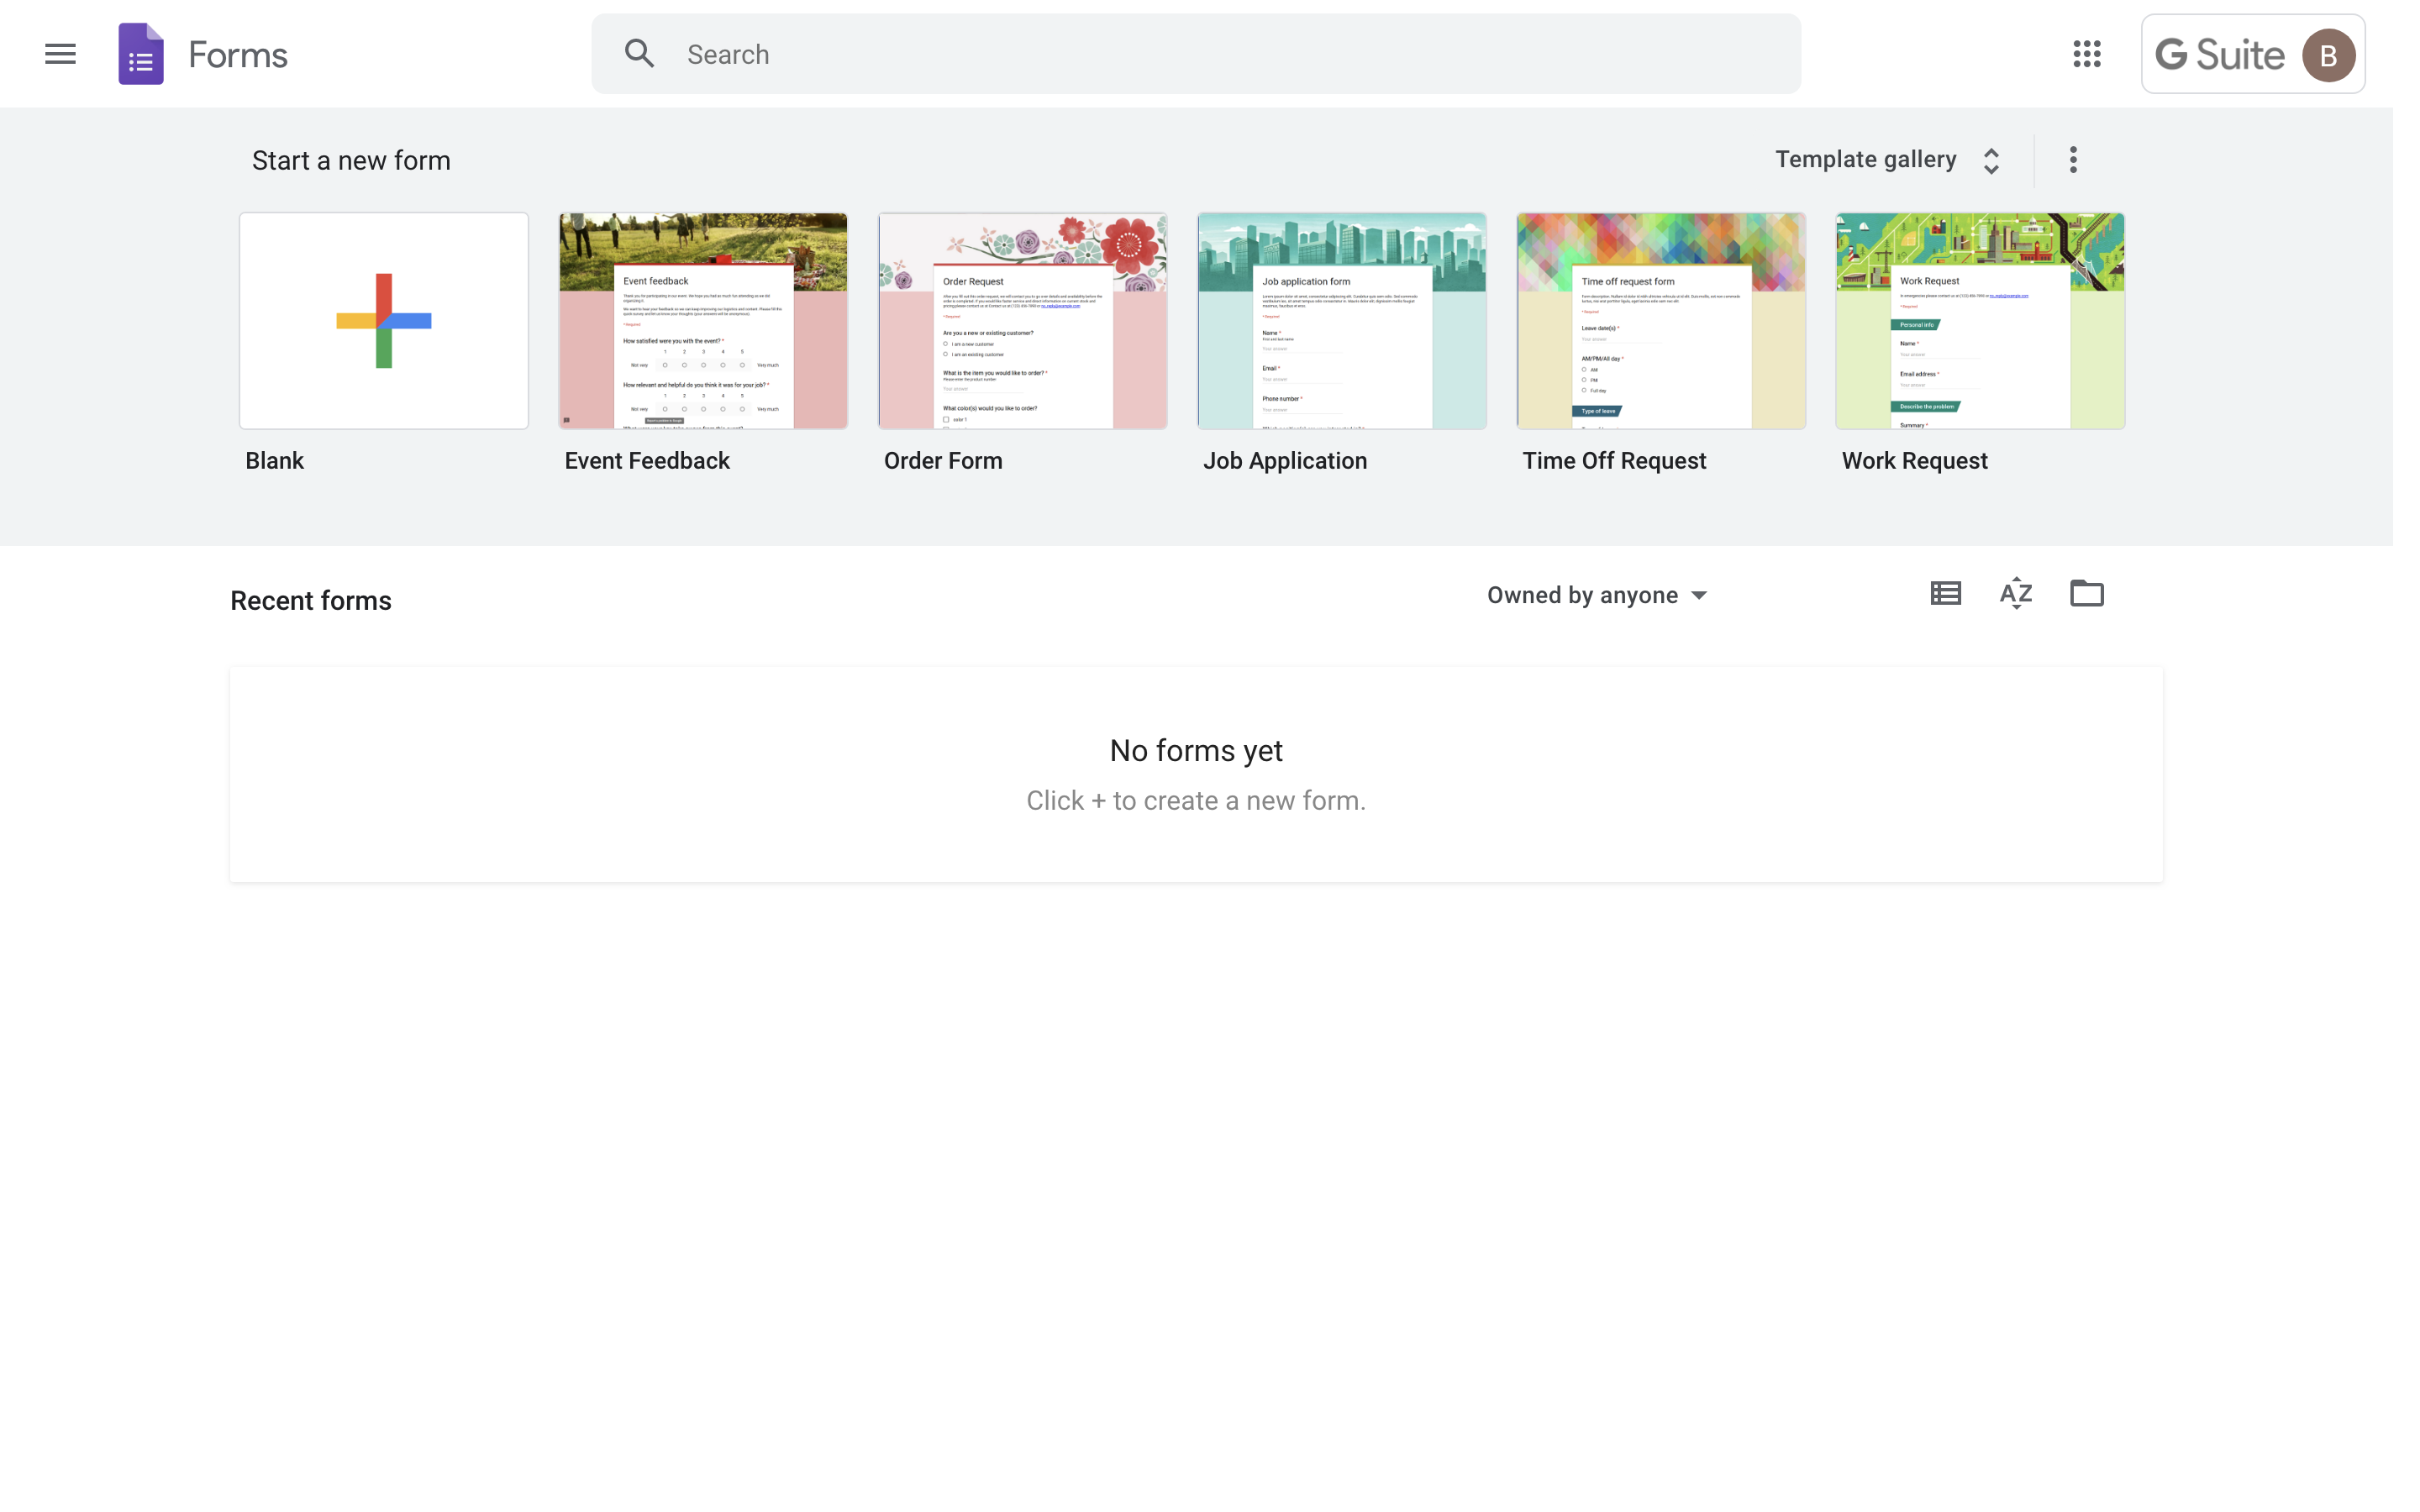
\includegraphics[width=1\textwidth]{img/gf/gf-dashboard}
		\caption{Google Form - Painel de Controlo}
		\label{fig:gf-dashboard}
	\end{center}
\end{figure}


\begin{figure}[ht!]
	\begin{center}
		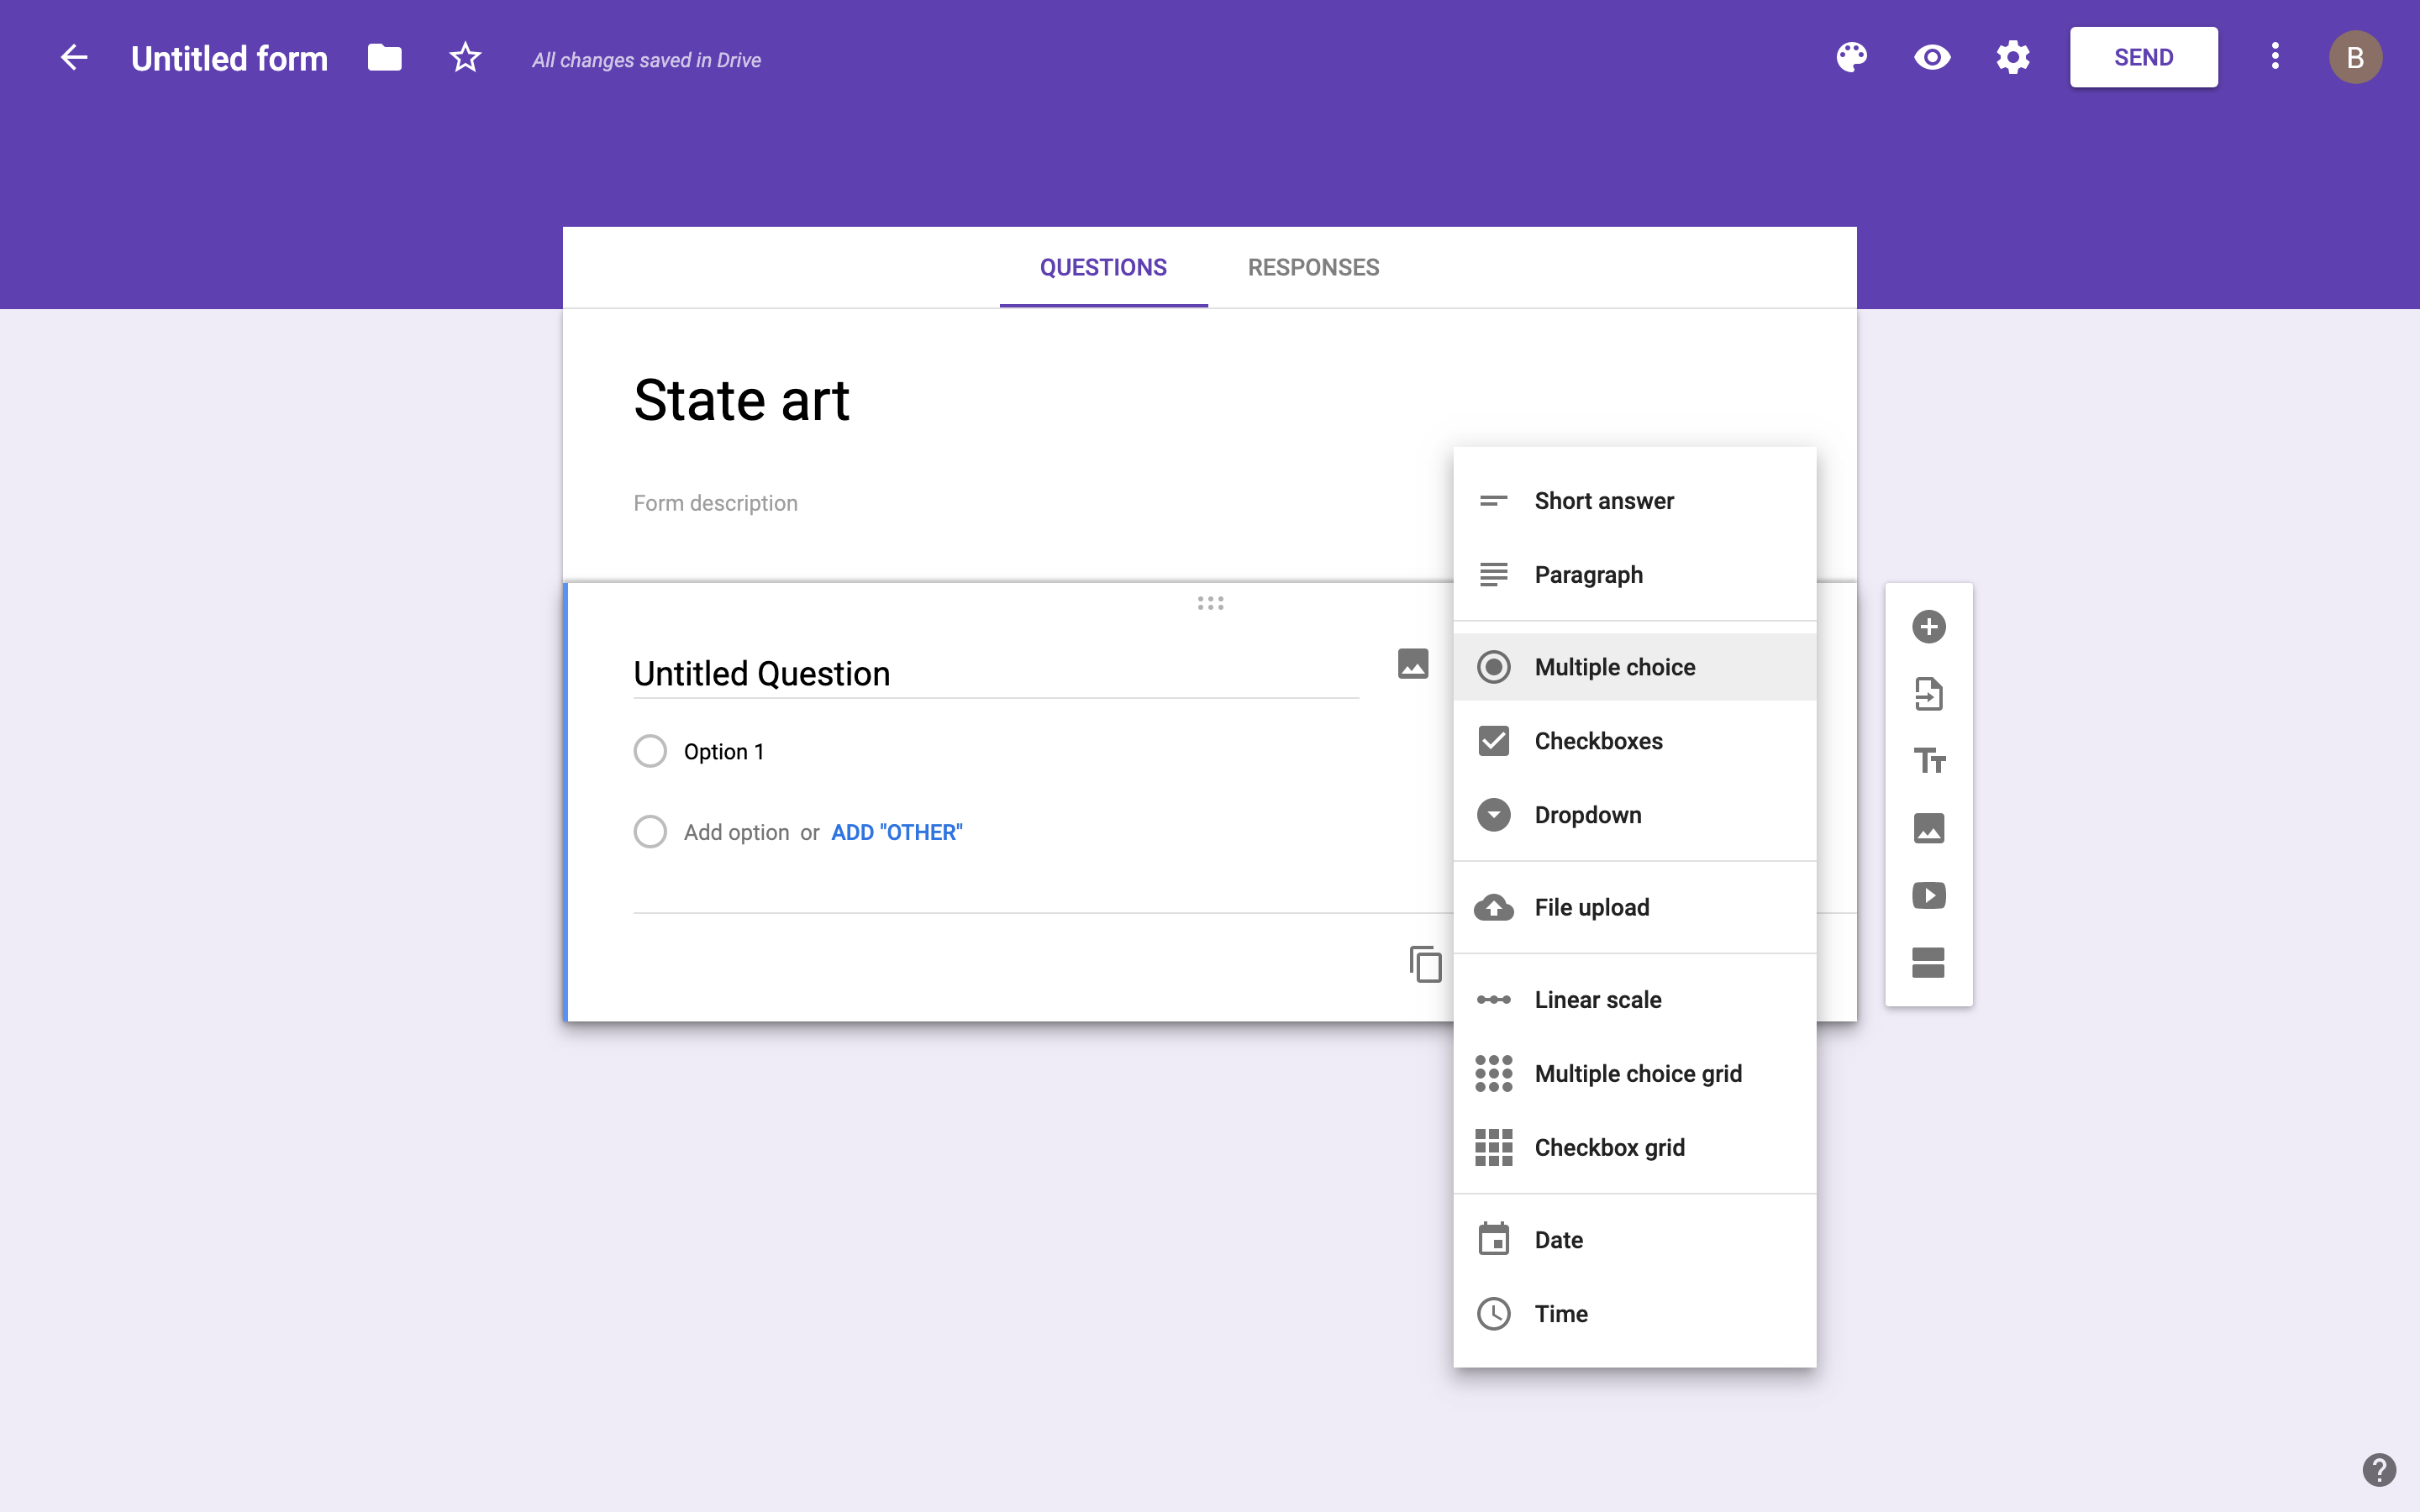
\includegraphics[width=1\textwidth]{img/gf/gf-form-q-type}
		\caption{Google Form - Tipos de perguntas}
		\label{fig:gf-form-q-type}
	\end{center}
\end{figure}

A Figura \ref{fig:gf-form-q-type} demonstra a criação de um formulário do zero. Há vários tipo de perguntas que a aplicação permite adicionar ao formulário e, apesar de se estar a criar um formulário novo, o google form permite importar um ou mais formulários diferentes, ao qual o utilizador tem acesso (i. e. formulários que estão disponíveis na sua área de trabalho), selecionando apenas as perguntas que deseja importar. Como podemos ver nas Figuras \ref{fig:gf-form-import}, \ref{fig:gf-form-import-select} e \ref{fig:gf-form-imported} as perguntas importadas foram colocadas na posição escolhida, que neste caso foi no final do formulário.

\begin{figure}[h!]
	\begin{center}
		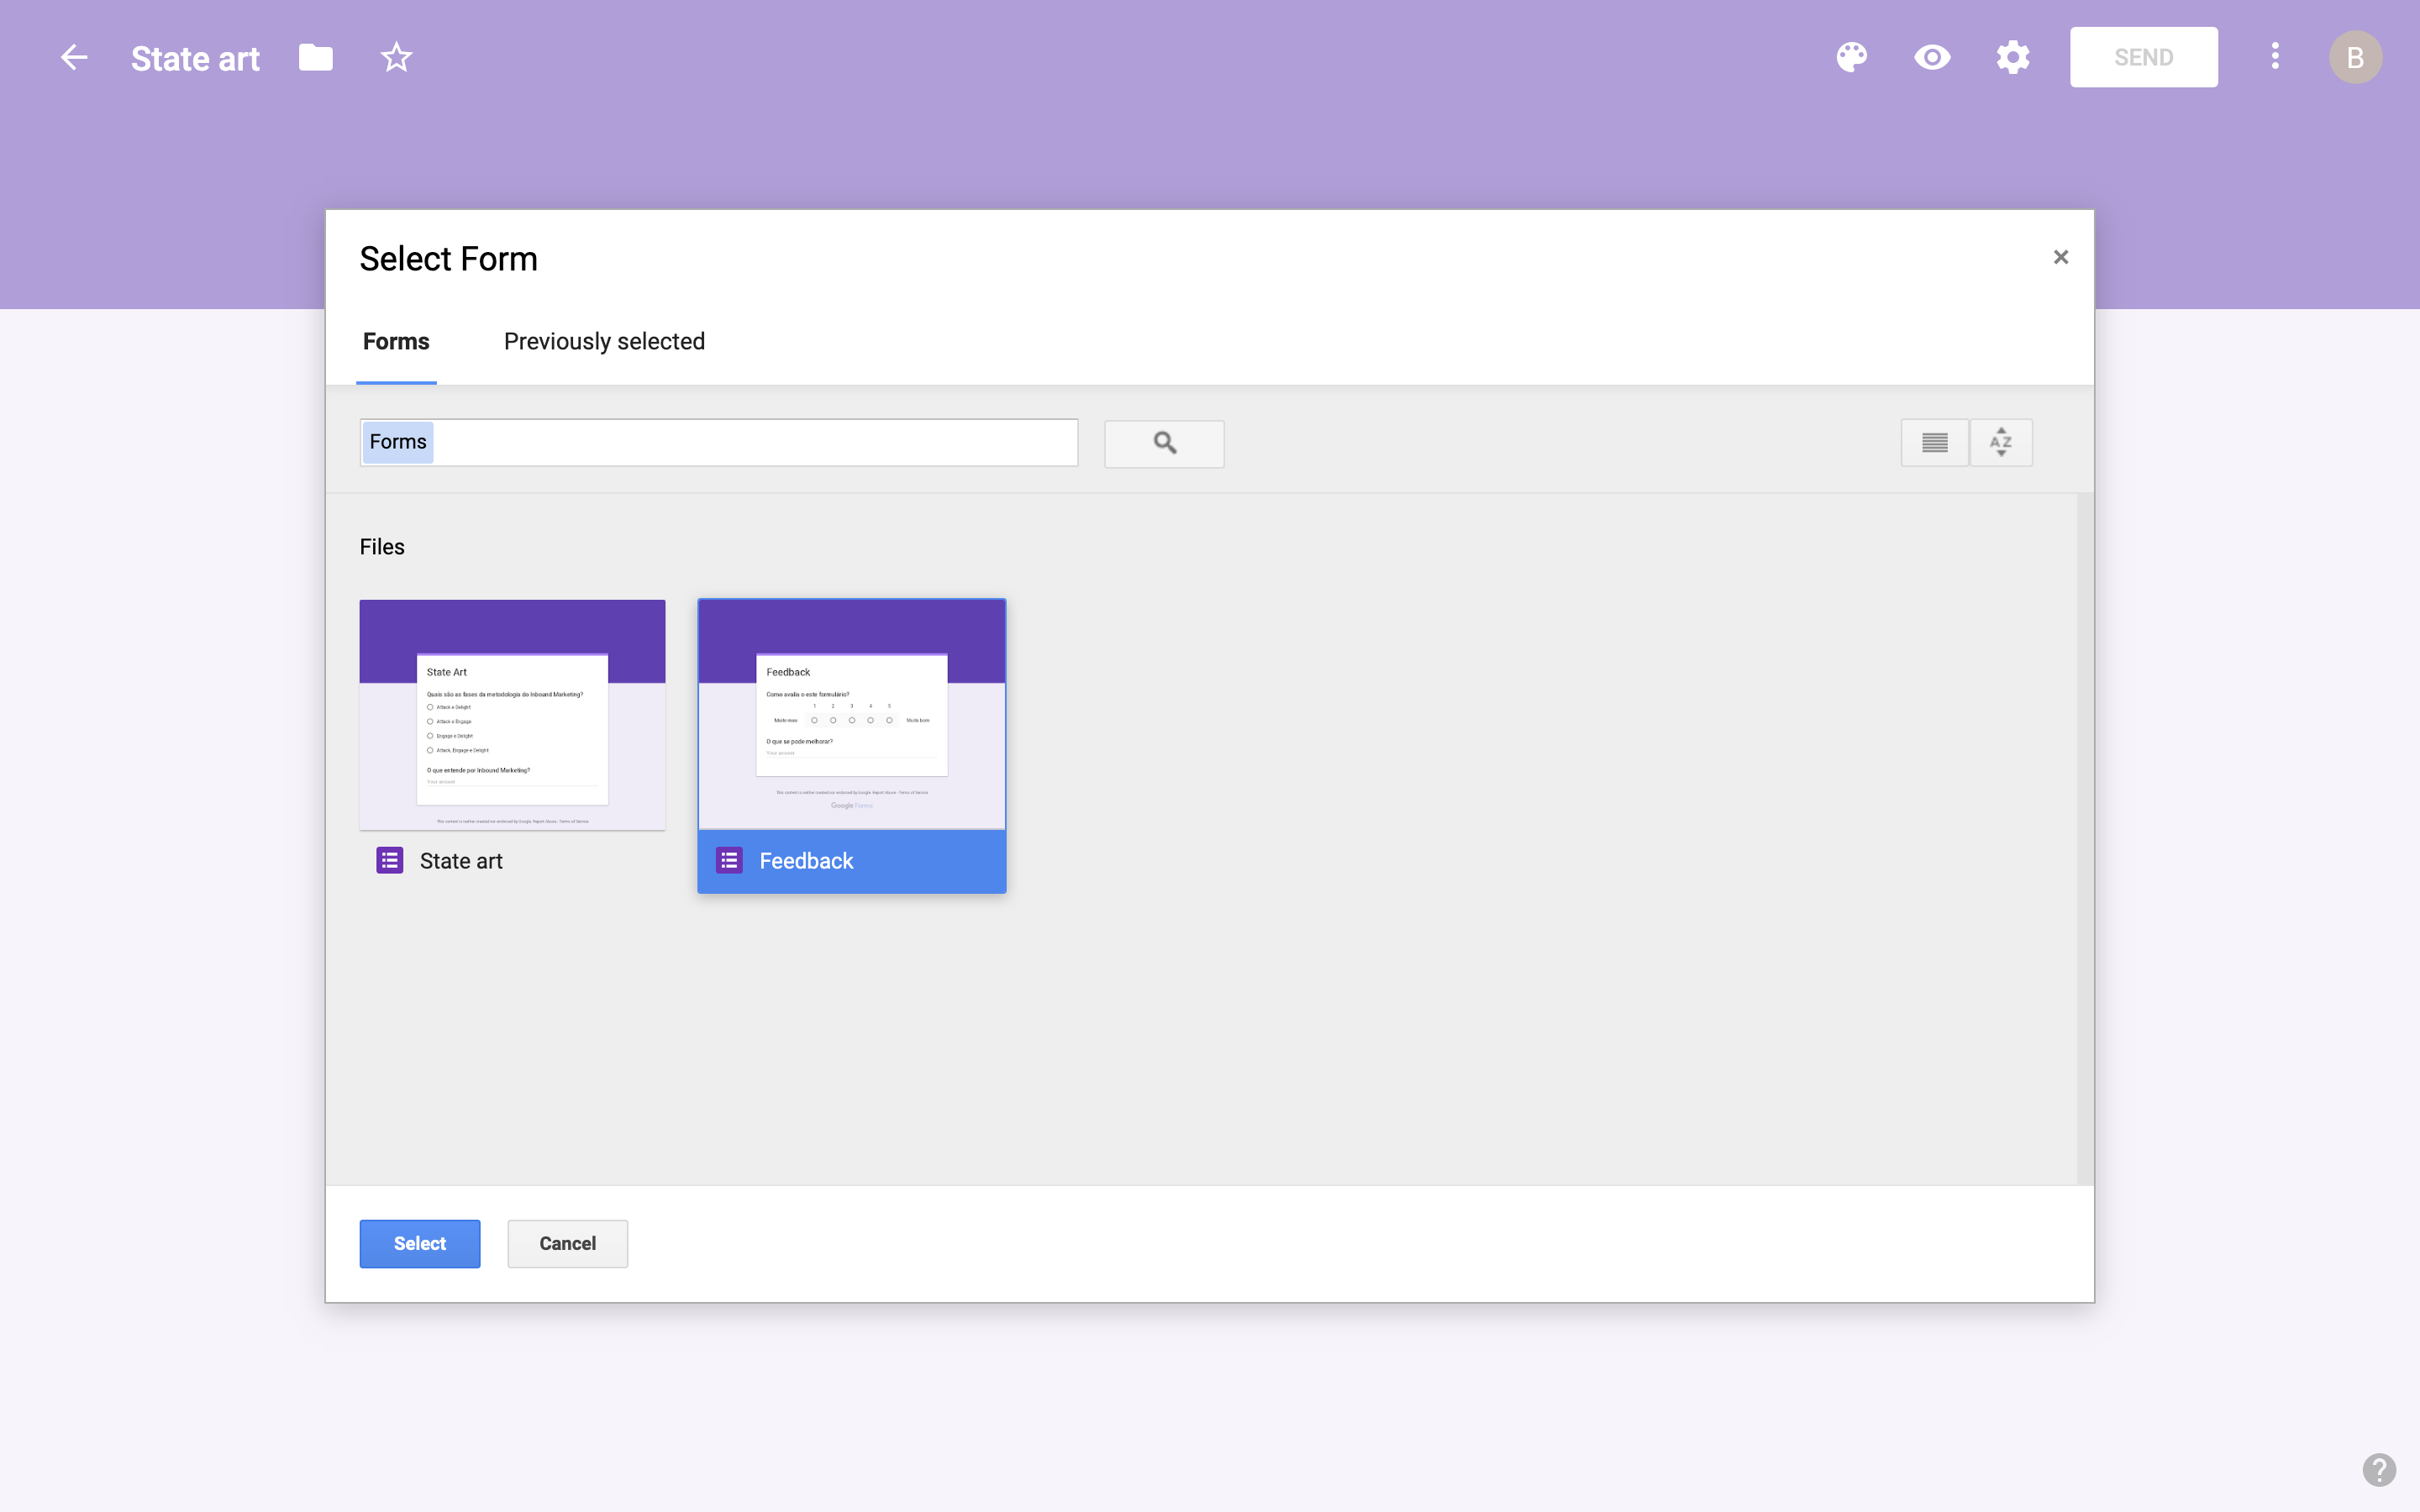
\includegraphics[width=1\textwidth]{img/gf/gf-form-import}
		\caption{Google Form - Importar formulário}
		\label{fig:gf-form-import}
	\end{center}
\end{figure}

\begin{figure}[h!]
	\begin{center}
		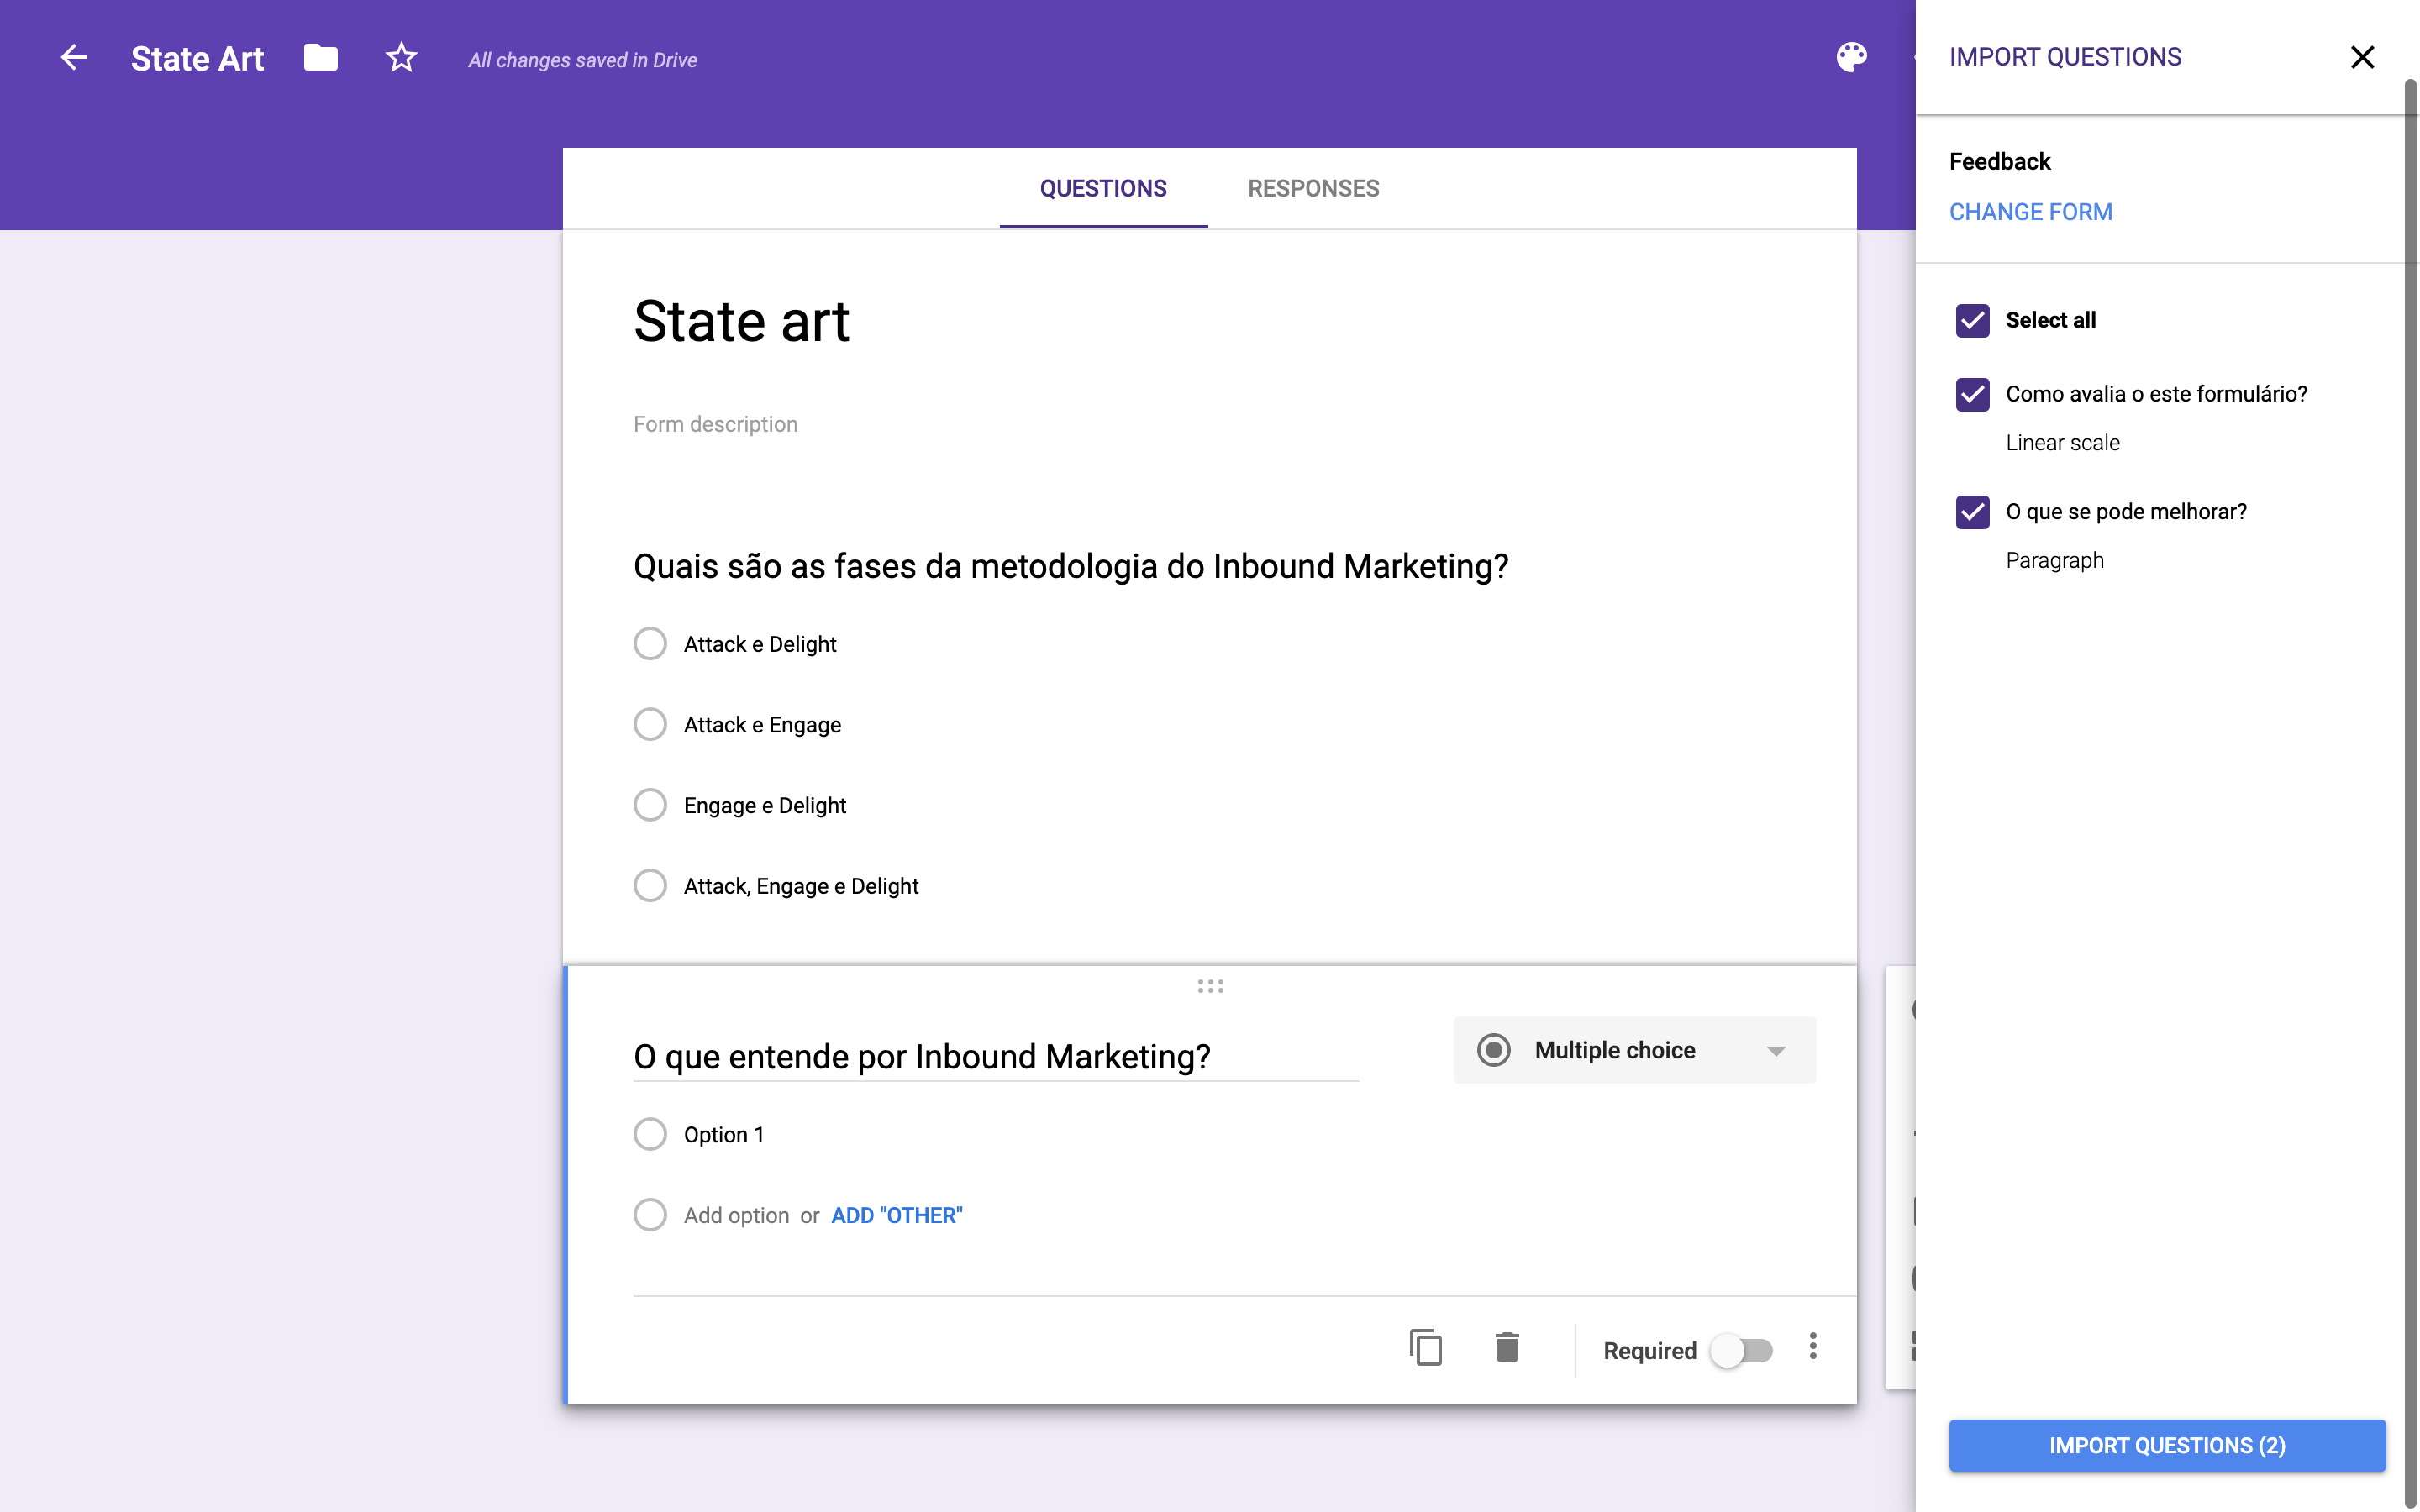
\includegraphics[width=1\textwidth]{img/gf/gf-form-import-select}
		\caption{Google Form - Selecionar perguntas a importar}
		\label{fig:gf-form-import-select}
	\end{center}
\end{figure}

\begin{figure}[h!]
	\begin{center}
		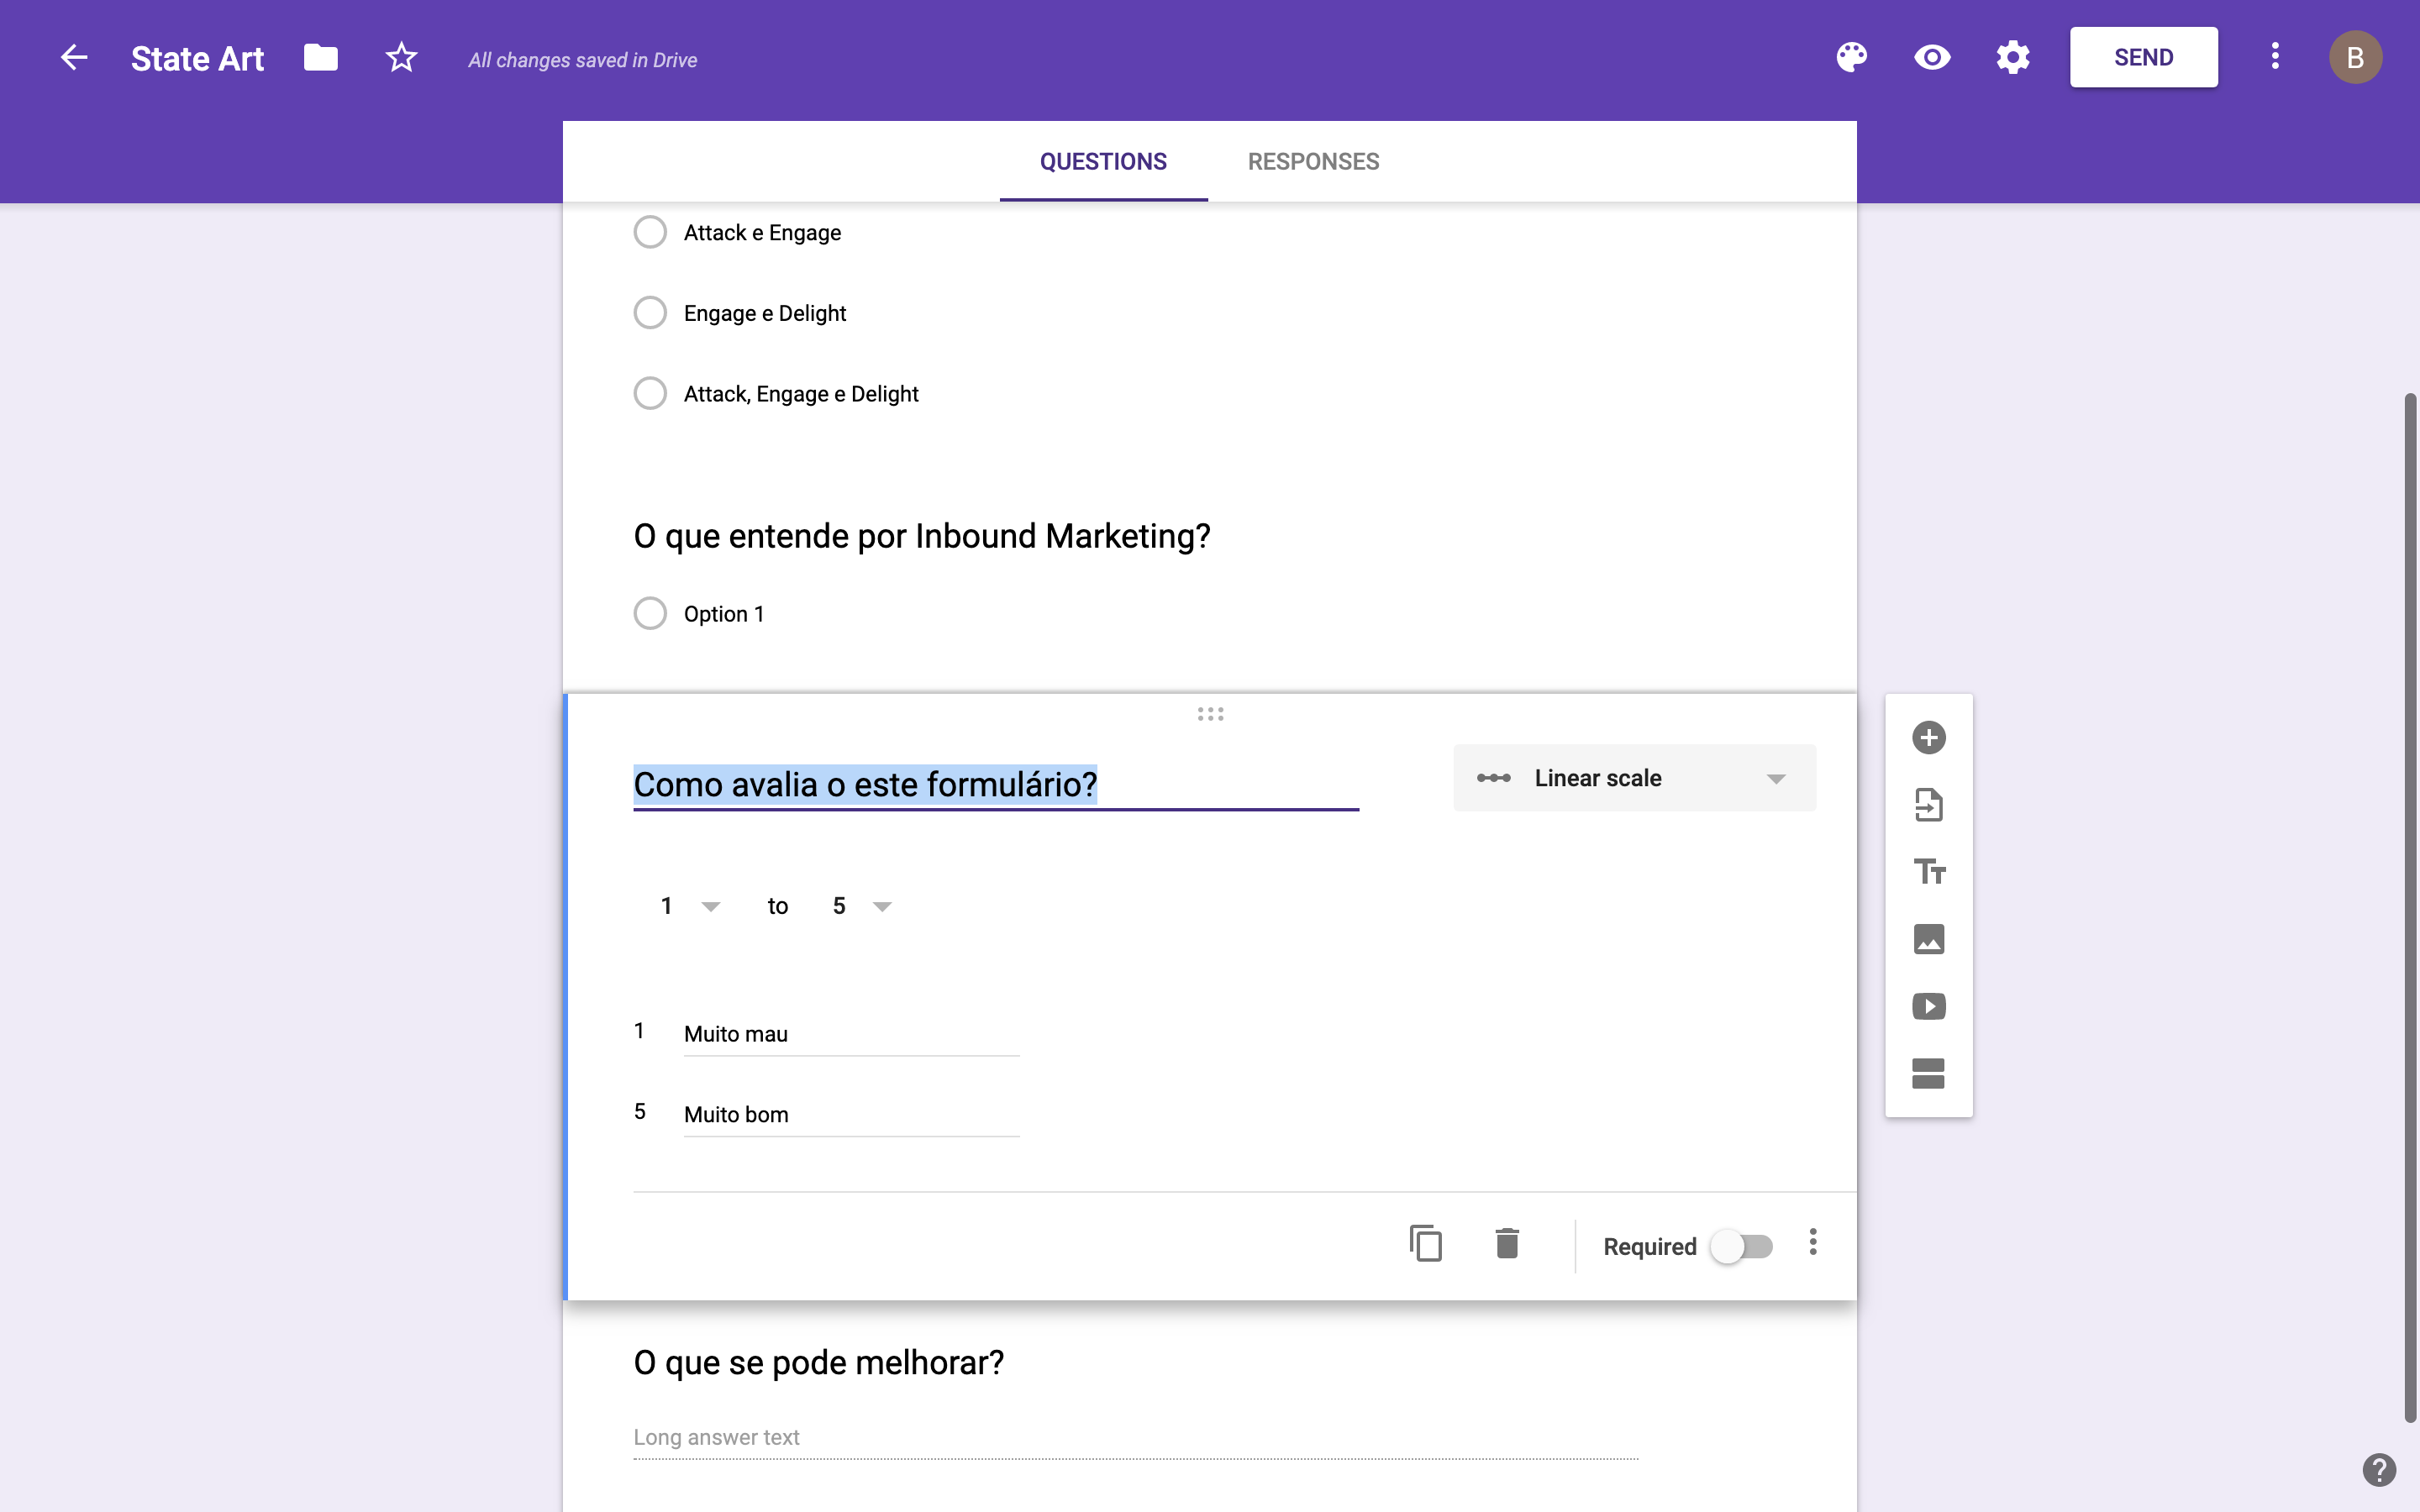
\includegraphics[width=1\textwidth]{img/gf/gf-form-imported}
		\caption{Google Form - Perguntas importadas}
		\label{fig:gf-form-imported}
	\end{center}
\end{figure}


\begin{figure}[h!]
	\begin{center}
		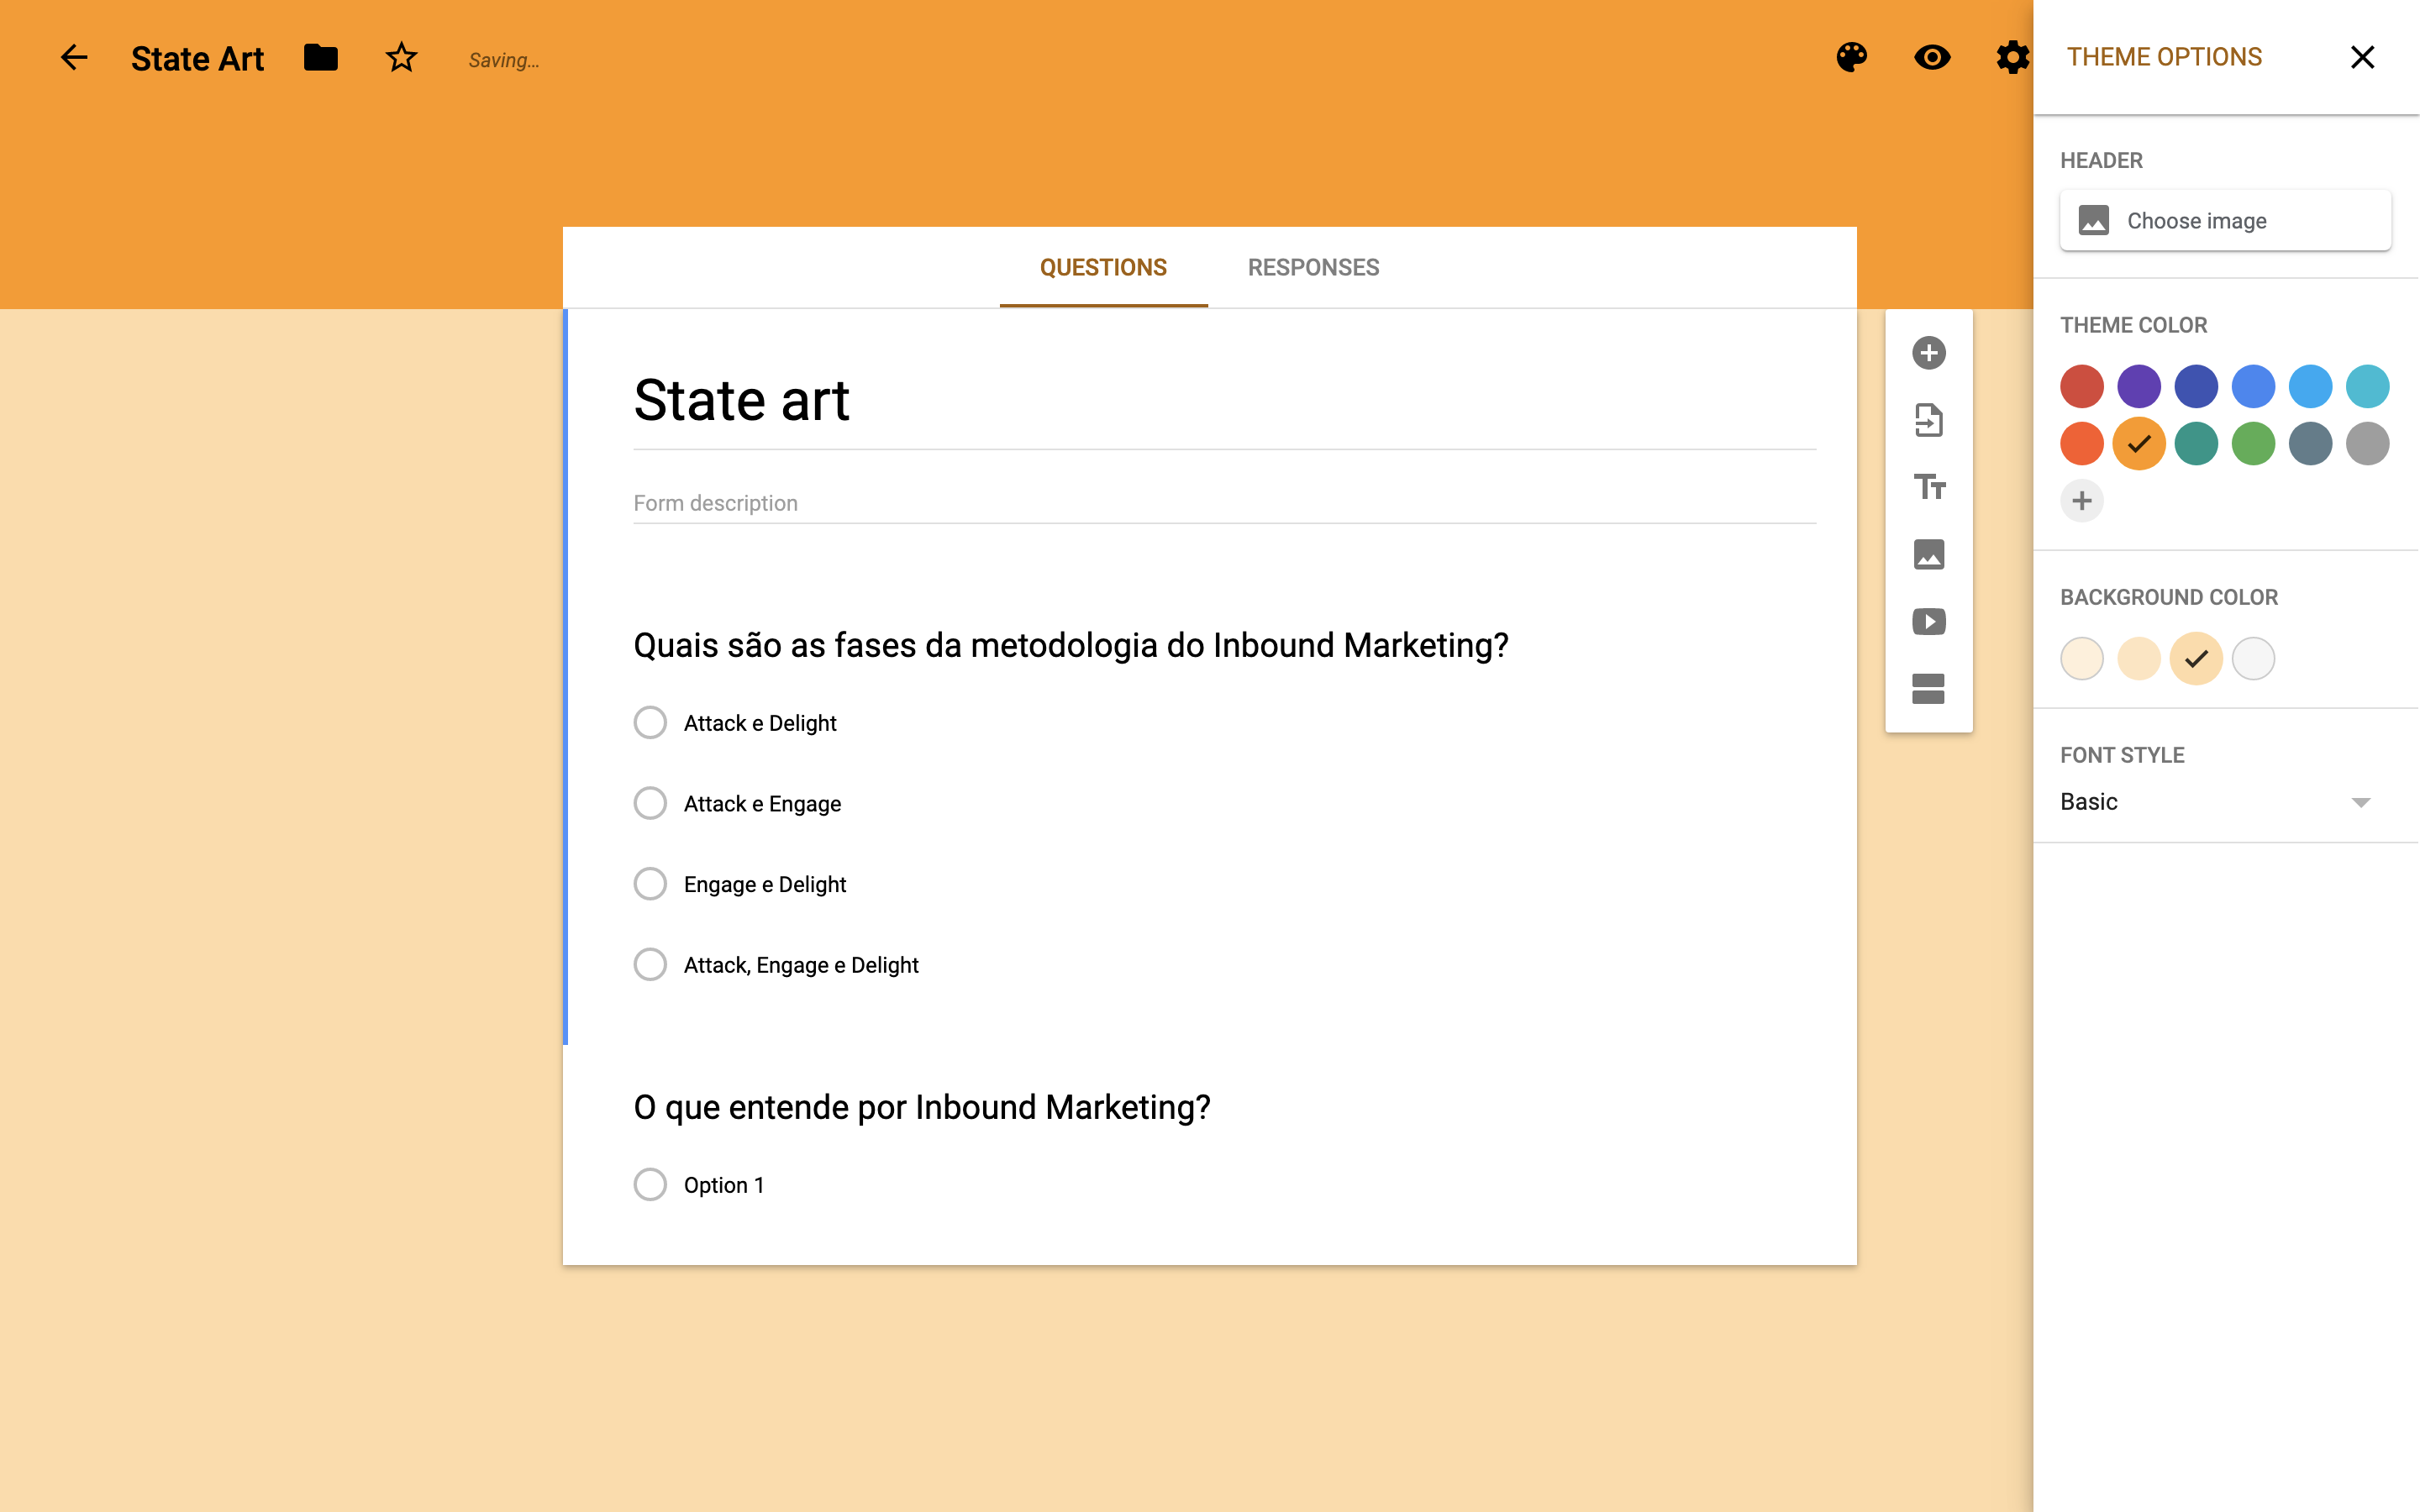
\includegraphics[width=1\textwidth]{img/gf/gf-form-design}
		\caption{Google Form - Alterar design do formulário}
		\label{fig:gf-form-design}
	\end{center}
\end{figure}

\newpage

Grande parte das plataformas e aplicações,no mercado, de criação de formulários permitem personalizar os formulários, ao gosto do utilizador, e o Google Form não é excepção. A aplicação permite alterar as definições padrão do formulário(Figuras \ref{fig:gf-form-set1}, \ref{fig:gf-form-set2} e \ref{fig:gf-form-set3}) e, apesar de se poder também personalizar o \textit{design} do formulário (\ref{fig:gf-form-design}), apenas podemos alterar a cor ou imagem de fundo e fonte de texto.

\begin{figure}[ht!]
	\begin{center}
		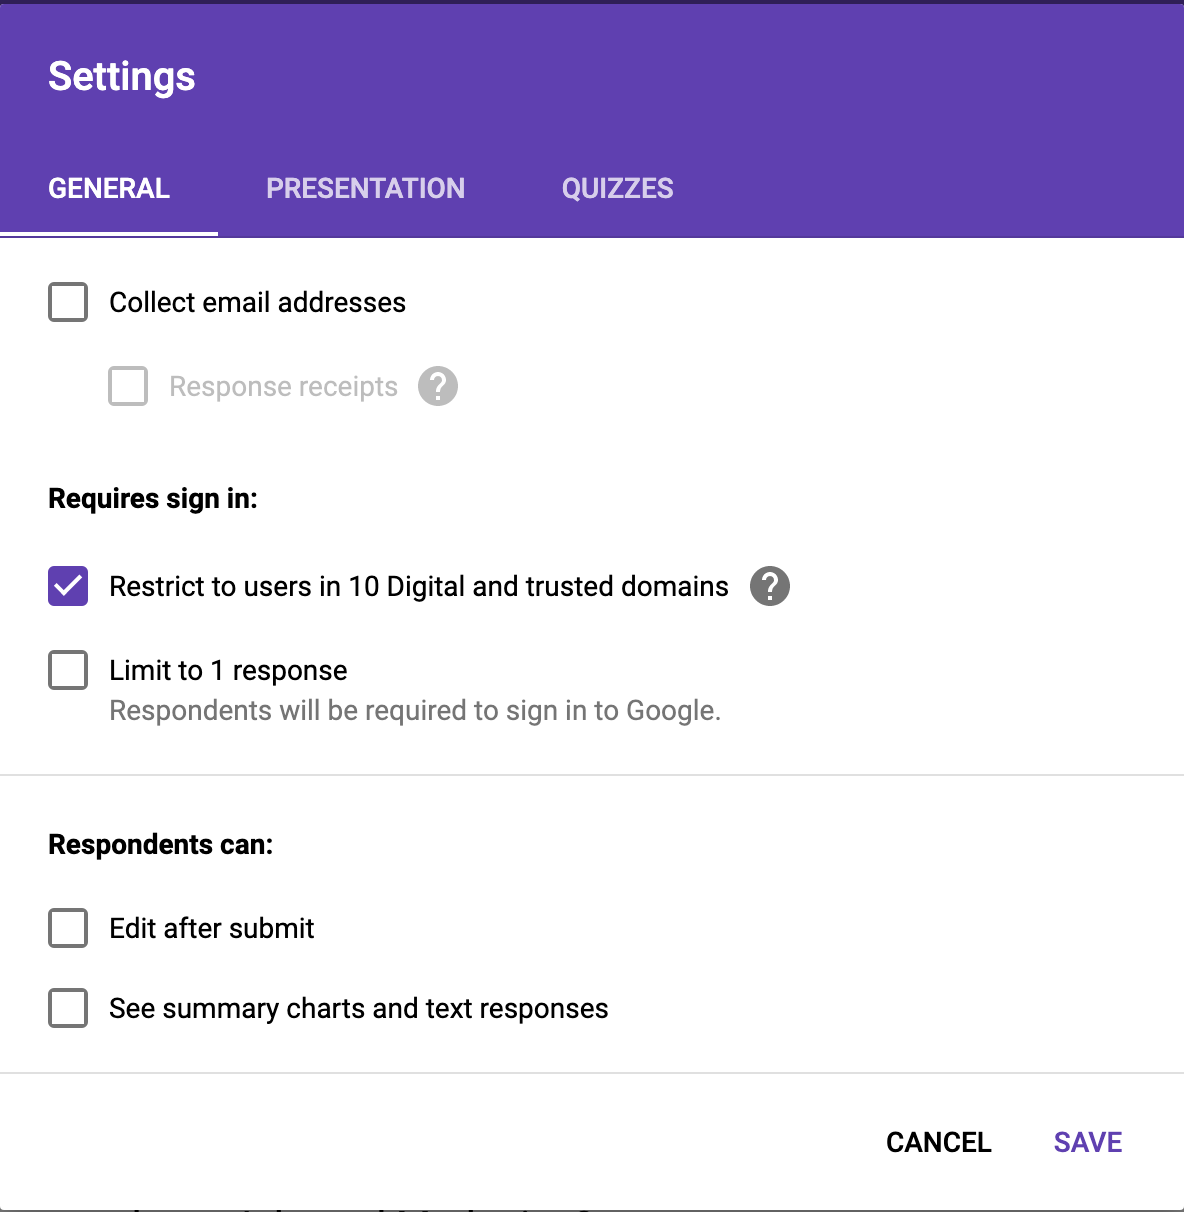
\includegraphics[height=.30\textheight]{img/gf/gf-form-set1}
		\caption{Google Form - Opções}
		\label{fig:gf-form-set1}
	\end{center}
\end{figure}

\begin{figure}[ht!]
	\begin{center}
		\begin{minipage}{0.40\textwidth}
			\begin{center}
				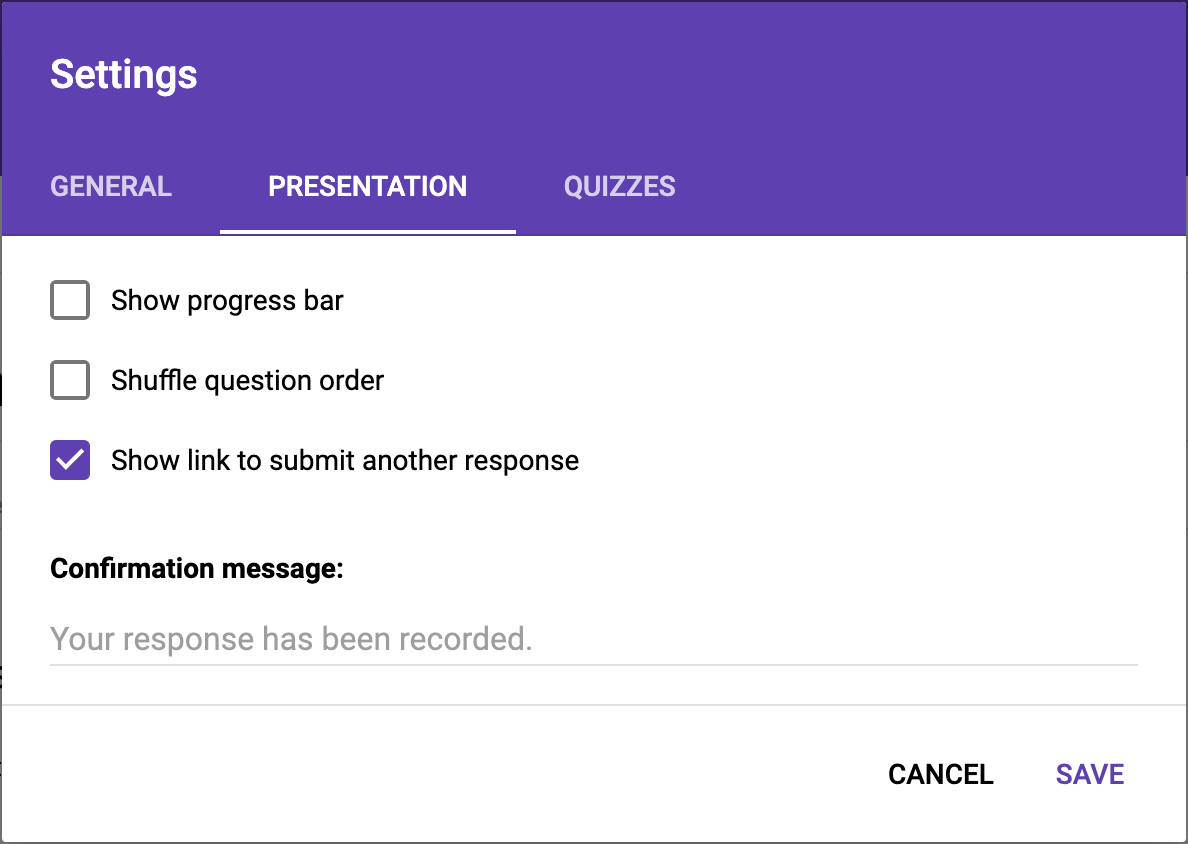
\includegraphics[height=.22\textheight]{img/gf/gf-form-set2}
				\caption{Google Form - Opções}
				\label{fig:gf-form-set2}
			\end{center}
		\end{minipage}
		\hspace{2cm}
		\begin{minipage}{0.40\textwidth}
			\begin{center}
				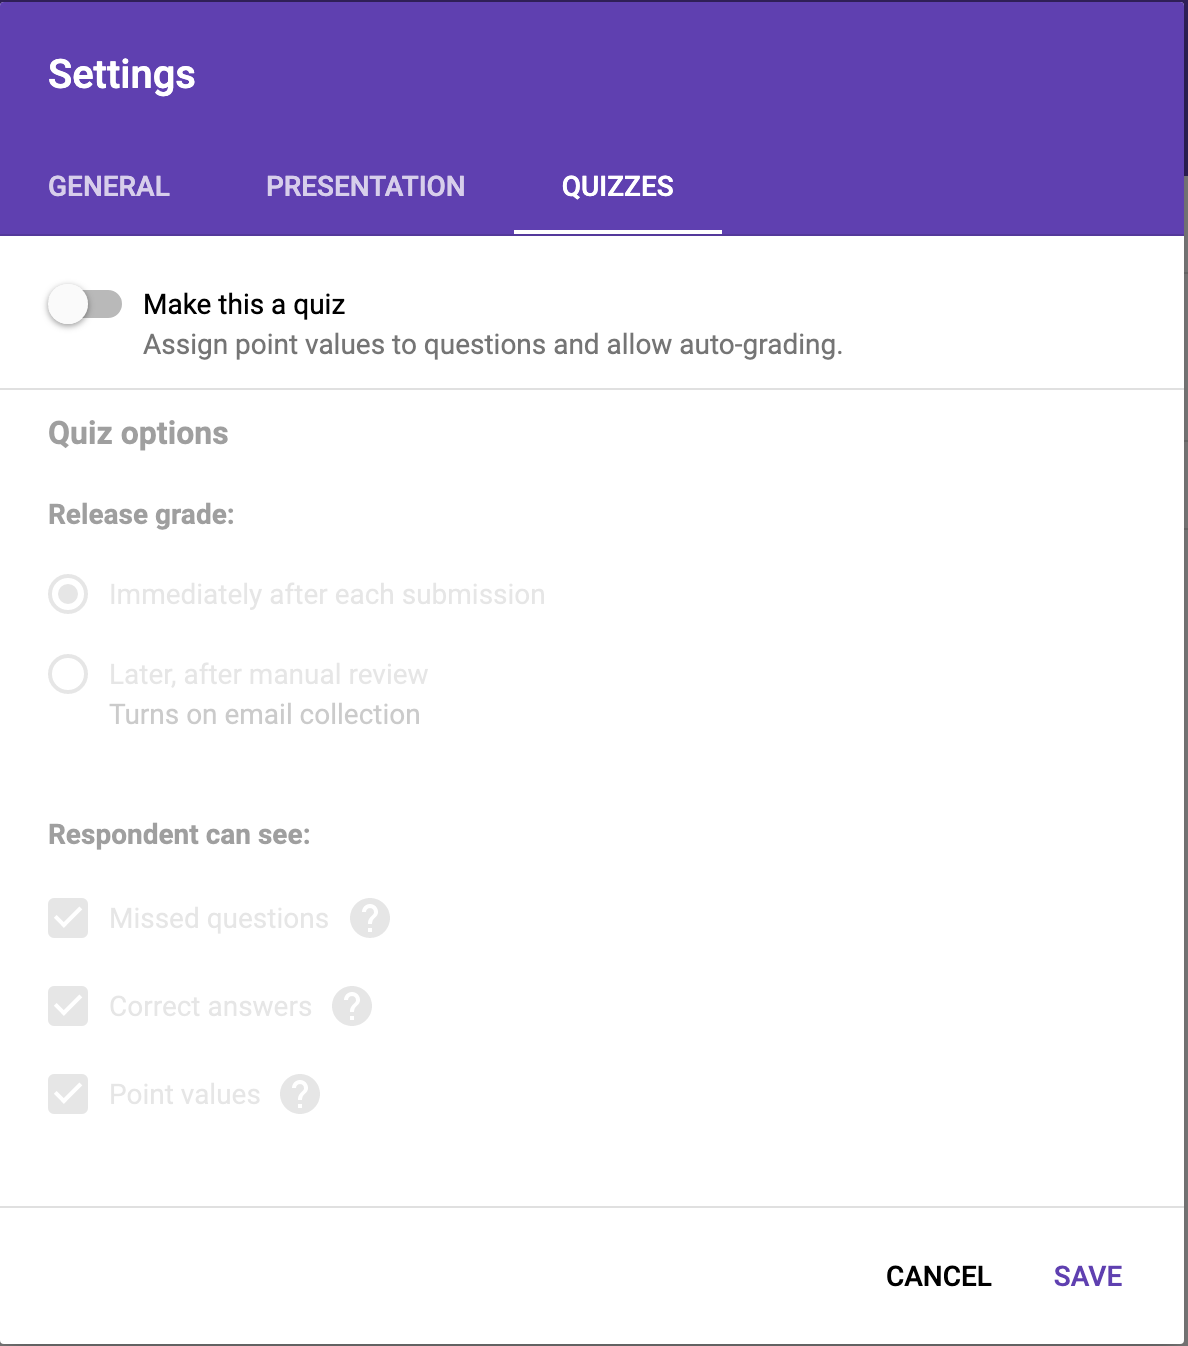
\includegraphics[height=.30\textheight]{img/gf/gf-form-set3}
				\caption{Google Form - Opções}
				\label{fig:gf-form-set3}
			\end{center}
		\end{minipage}
	\end{center}
\end{figure}

Antes de partilhar o formulário, precisamos de verificar se o formulário foi construído como planeado e para isso a aplicação fornece a funcionalidade: \textit{preview}. O Google Form permite os utilizadores enviarem o formulário através de um link, por email, embebido numa página web ou partilhando no Facebook ou Twitter utilizando os botões de partilha rápida.

Na análise de resultados, como podemos ver na Figura \ref{fig:gf-form-results} a aplicação faz uma exibição do resumo das respostas, mostrando alguns gráficos/estatísticas contudo, o utilizador não dispõe de nenhuma funcionalidade que filtra ou segmenta os dados. A única maneira que o utilizador tem de poder tratar os dados e segmentá-los é, depois de exportar os dados, utilizando o Google Sheets, que já requer algum conhecimento na ferramenta. 

\newpage
\mbox{}

\begin{figure}[ht!]
	\begin{center}
		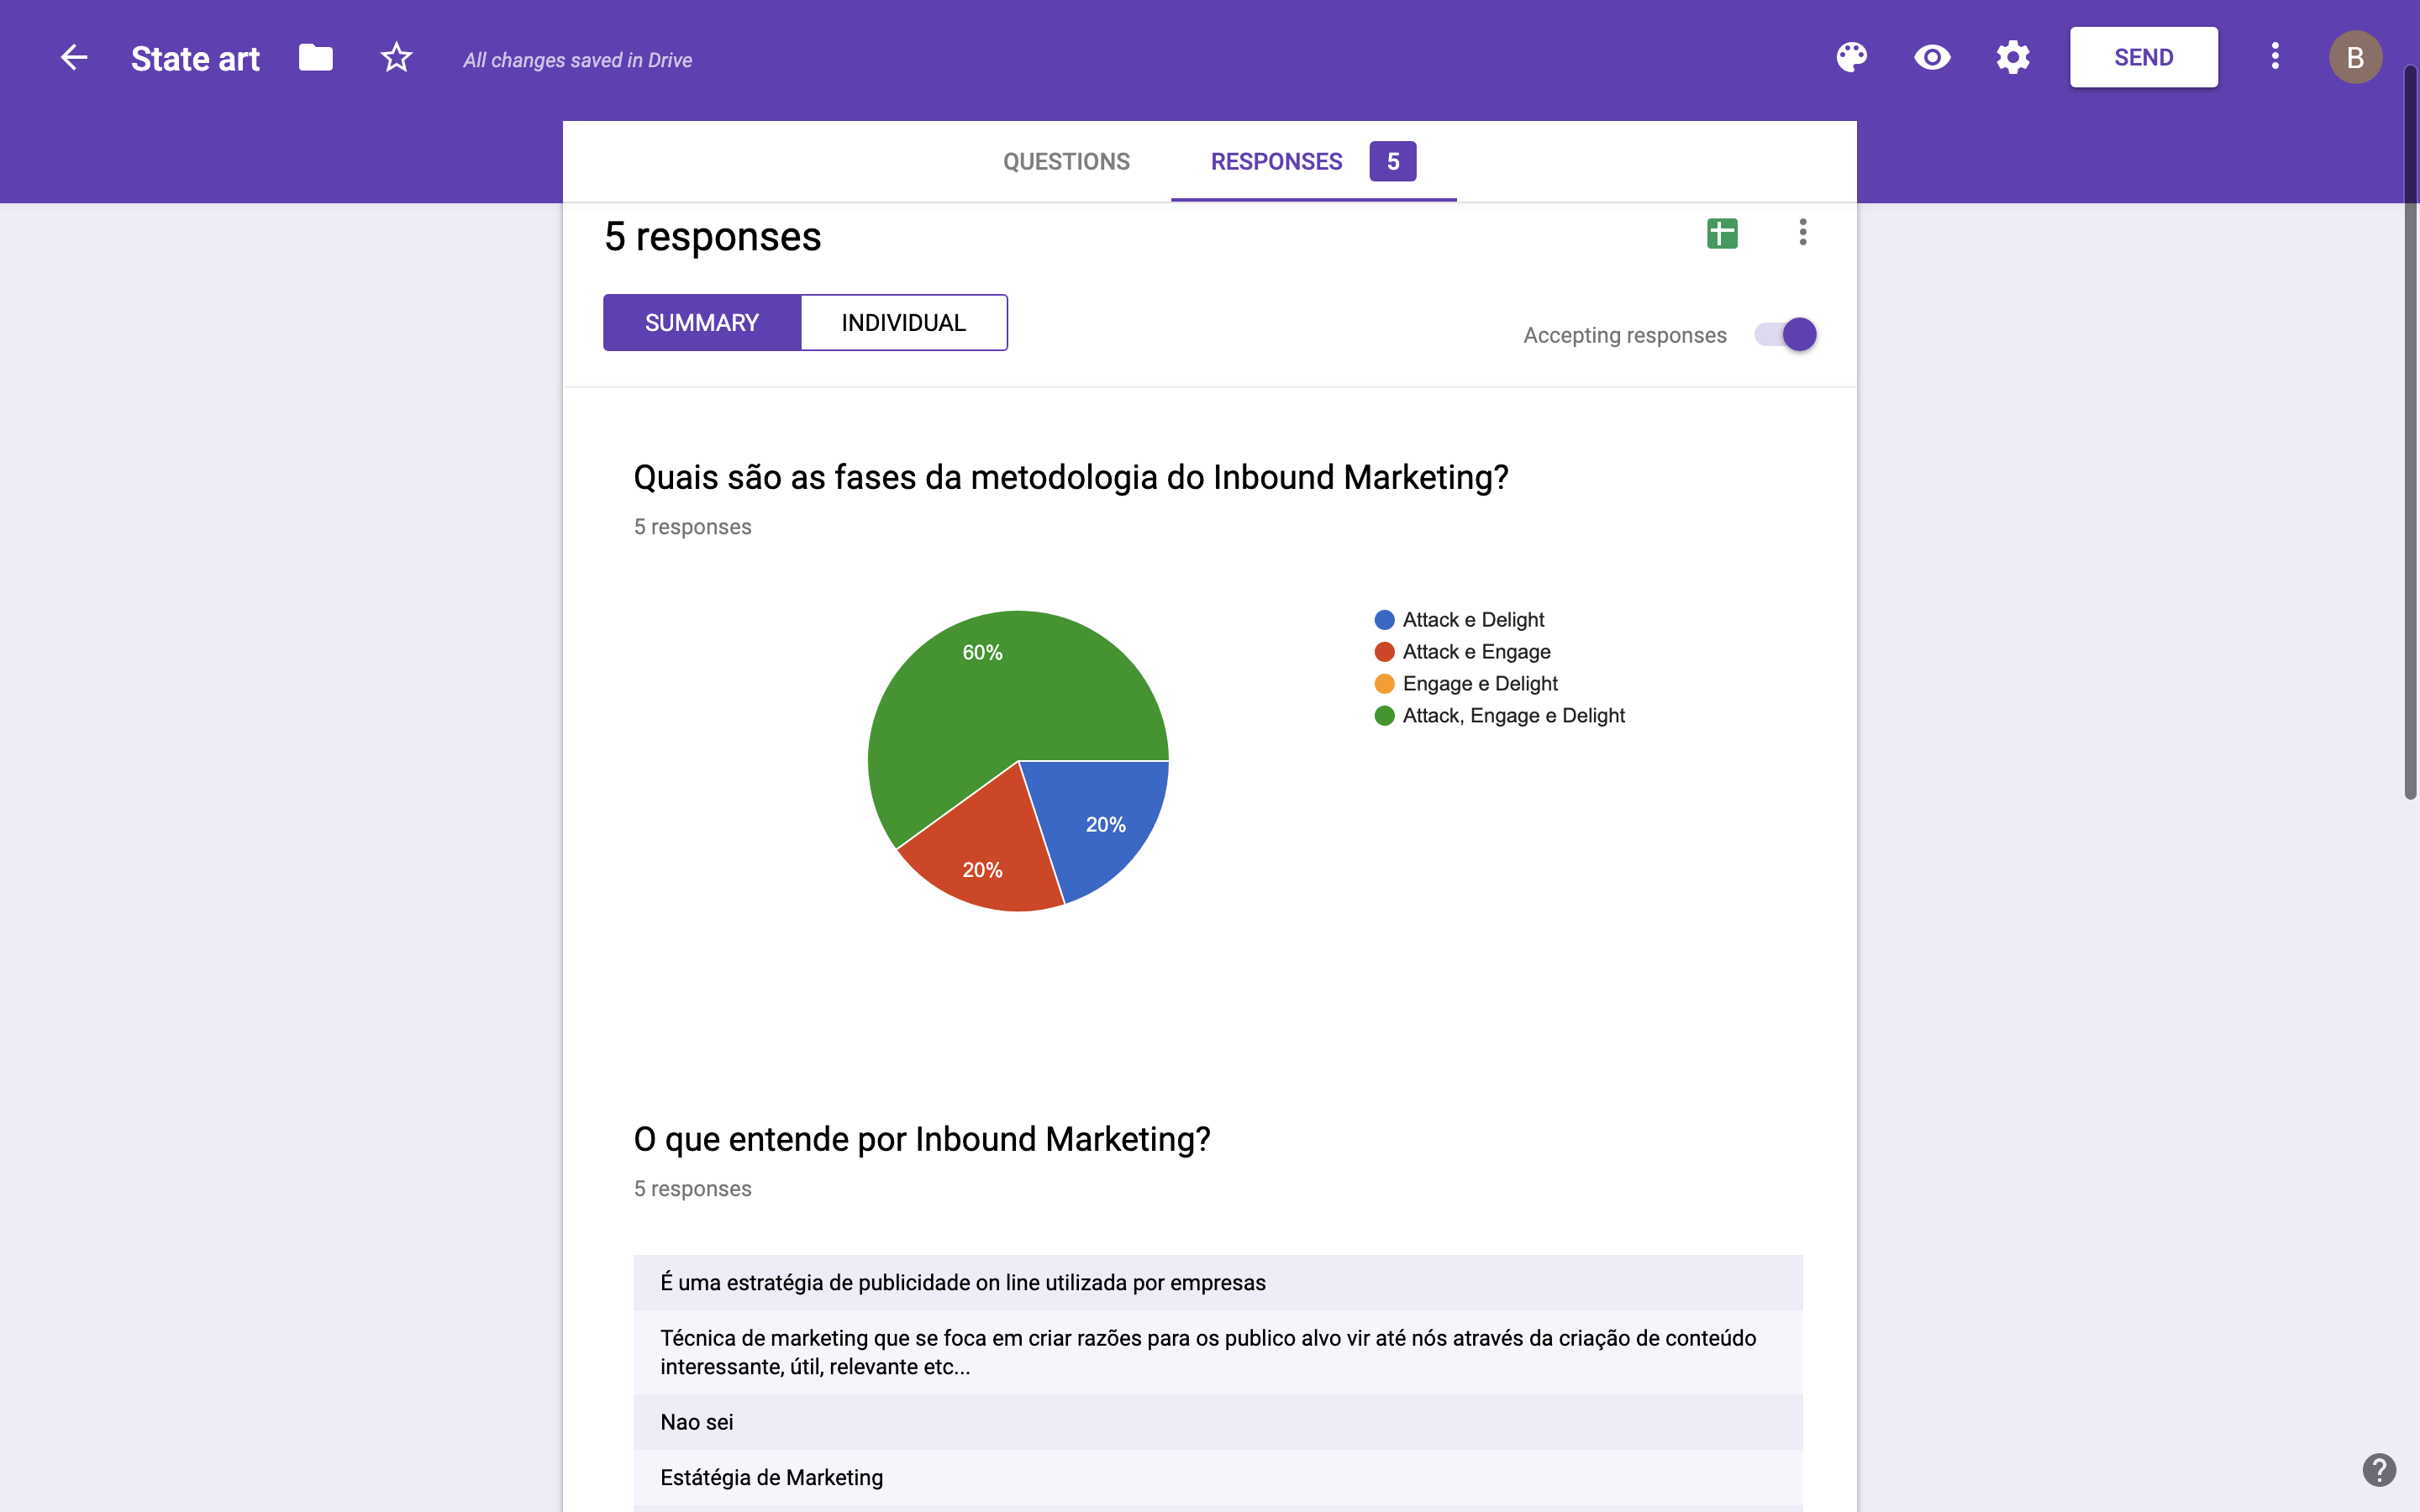
\includegraphics[width=1\textwidth]{img/gf/gf-form-results}
		\caption{Google Form - Sumério dos resultados obtidos}
		\label{fig:gf-form-results}
	\end{center}
\end{figure}

\section{\acrfull{tcg}}
\label{sec:TCG}

O \acrlong{tcg} é um produto actualmente no mercado, desenvolvido pela equipa da 10.digital, que tem como principal objectivo transformar PDFs numa aprendizagem baseada em tentativa erro. O \acrshort{tcg} nasceu de uma forte convicção de que perder apenas 2 minutos por dia numa formação tentativa erro é uma óptima forma de aprender, poupando tempo e dinheiro às empresas. Inicialmente muito focado em formação interna, a equipa do \acrshort{tcg} foi-se apercebendo que existem muitos outros problemas (e. g. Consolidação de procedimentos, \textit{Onboarding} de novos colaboradores, Divulgação da cultura da empresa, Divulgação de informações técnicas a parceiros/clientes ...) para o qual a plataforma tem solução (e. g. Assimilação da cultura de empresa e do espírito das marcas, Simplificação do processo de acolhimento, Redução de custos em reuniões periódicas, Facilidade em divulgar aspectos técnicos, que de outra, forma demorariam mais tempo ...).\cite{tcginfo}

O \acrshort{tcg} é um \acrshort{saas} pago que disponibiliza uma demo de 30 dias. Esta demo permite ao utilizador utilizar todas as funcionalidades da plataforma e, tal como nos planos pagos, disponibiliza ainda um tutorial de como efectuar as actividades chaves.

Este produto permite-nos criar utilizadores finais (i. e. quem irá responder à formação), questões e formações. As questões e os utilizadores finais, são categorizados através de tags, optimizando assim a forma como associamos os mesmos a uma formação nova ou já existente, como veremos em diante.

Como podemos ver na Figura \ref{fig:tcg-homepage} na página inicial, a plataforma expõem algumas estatísticas gerais sobre as formações do utilizador.

\newpage


\begin{figure}[ht!]
	\begin{center}
		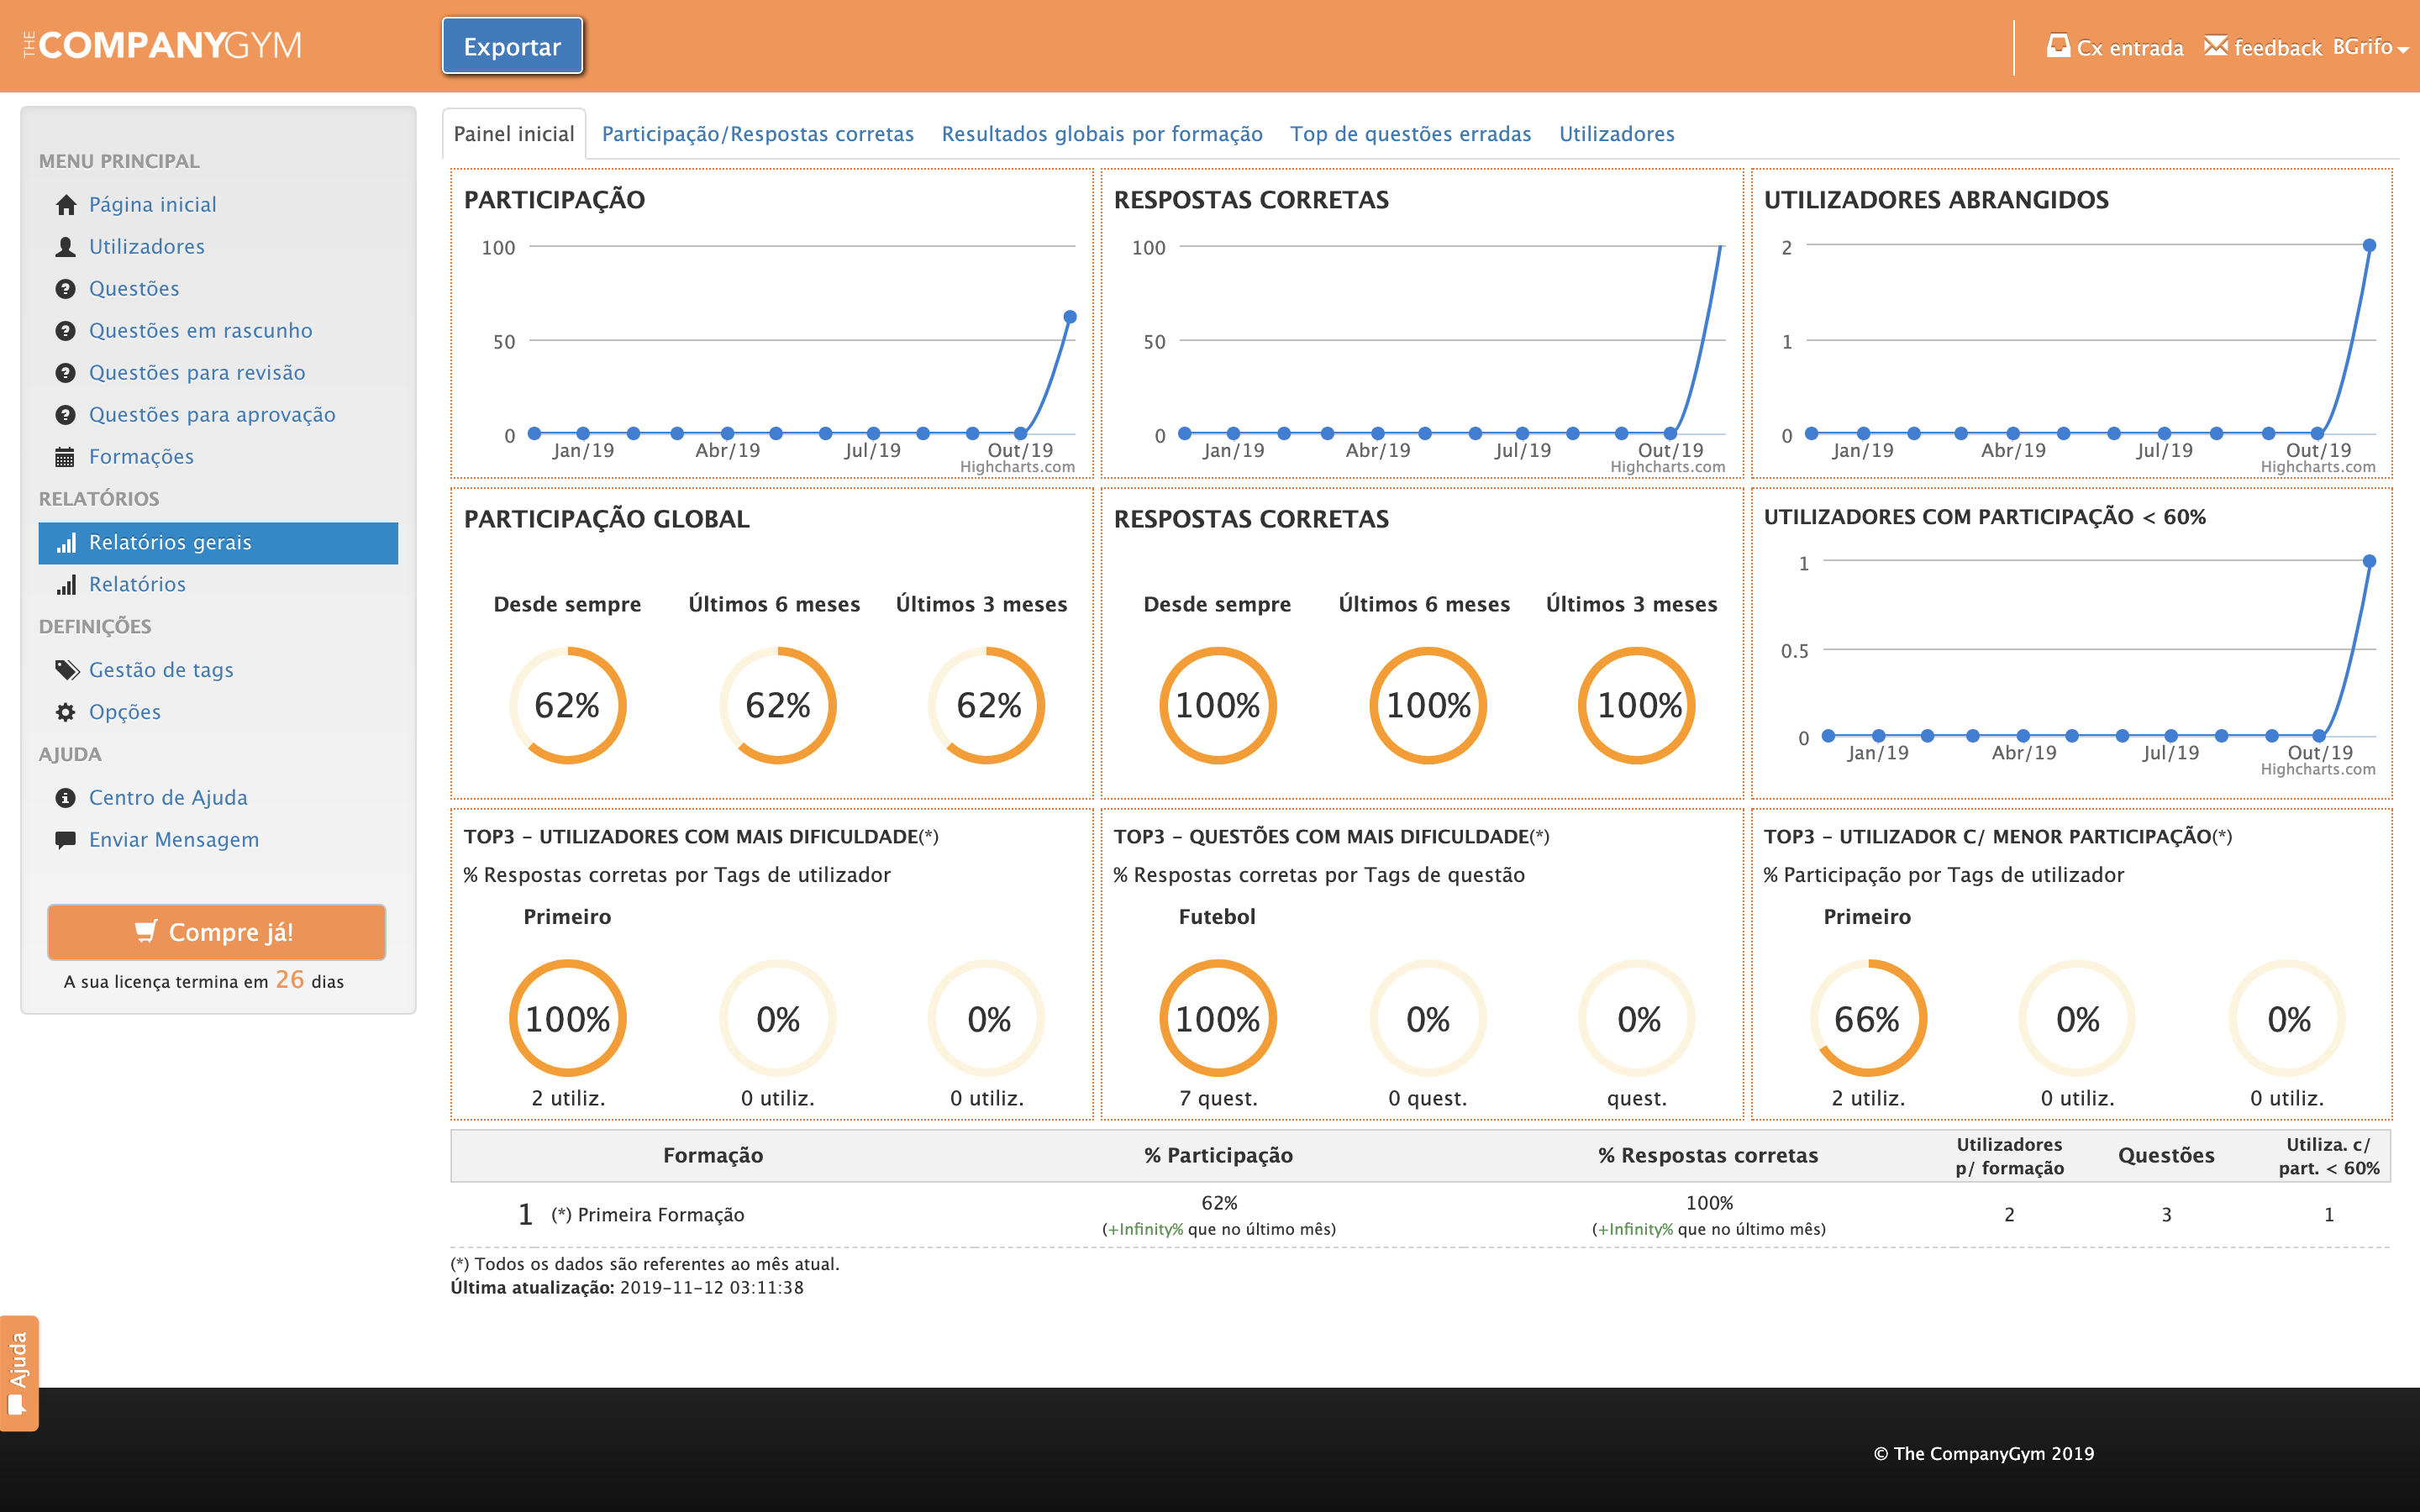
\includegraphics[width=1\textwidth]{img/tcg/tcg-homepage.png}
		\caption{The Company Gym - Página Inicial}
		\label{fig:tcg-homepage}
	\end{center}
\end{figure}

\begin{figure}[ht!]
	\begin{center}
		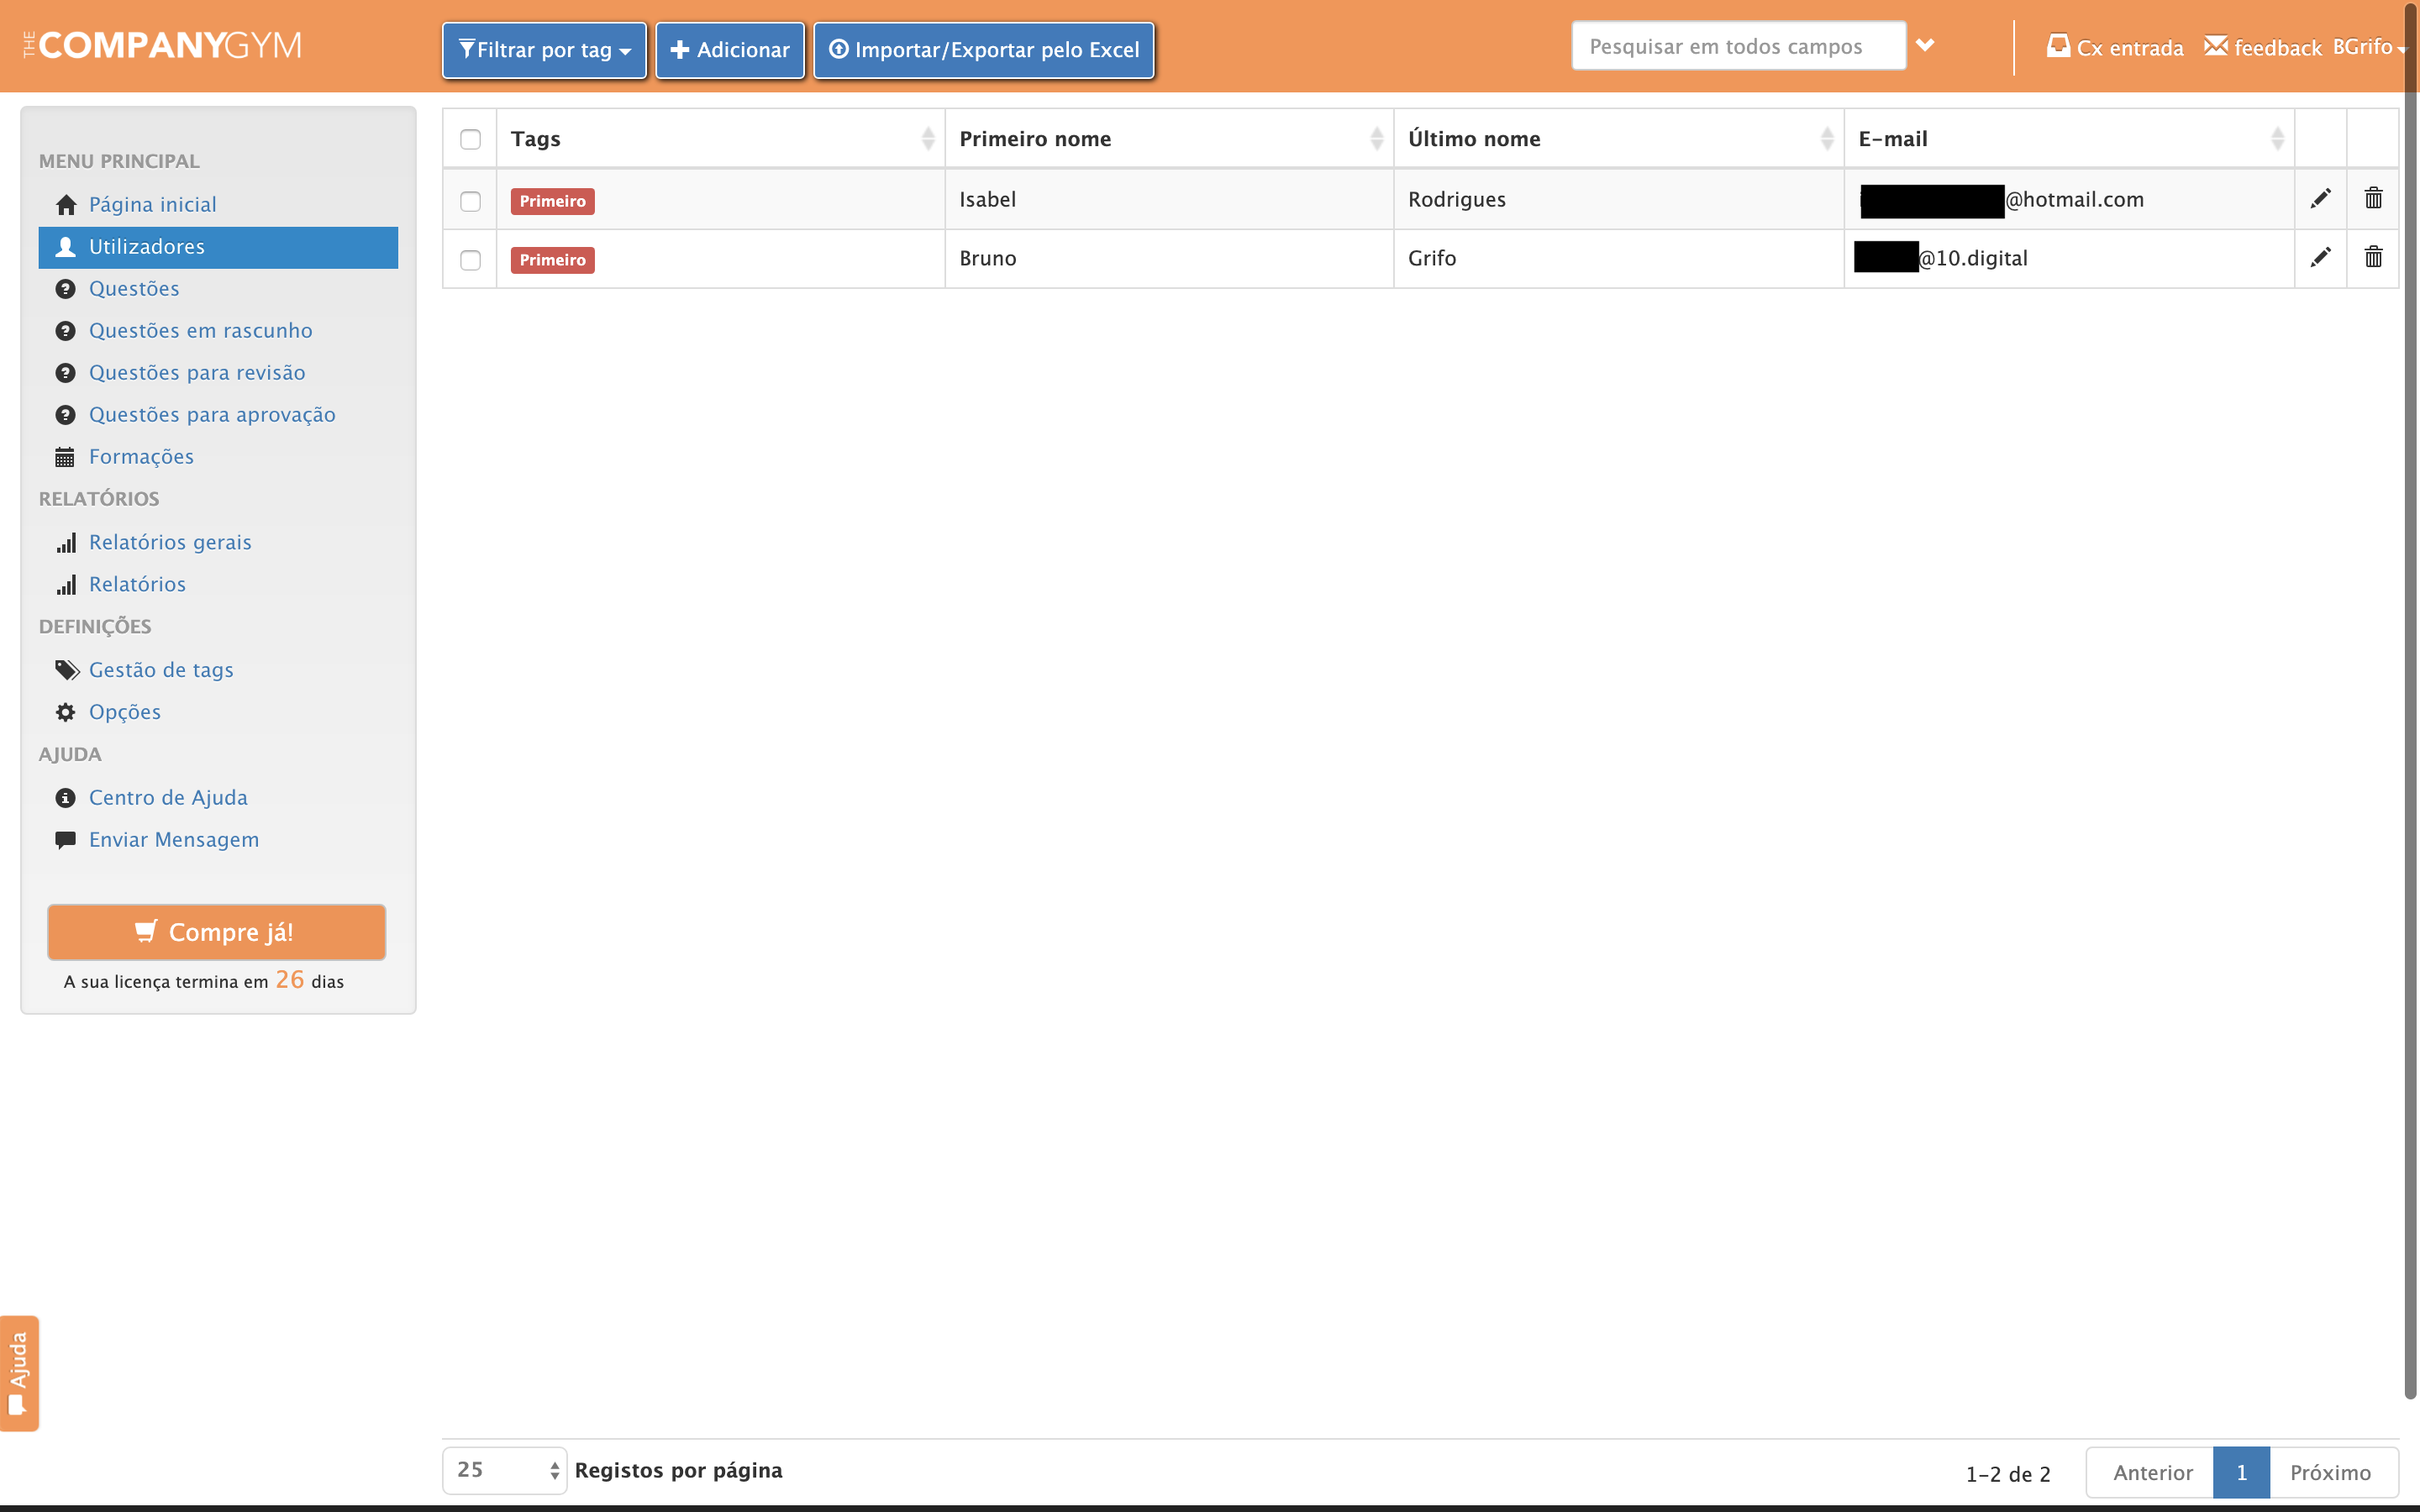
\includegraphics[width=1\textwidth]{img/tcg/tcg-utilizadores.png}
		\caption{The Company Gym - Lista de utilizadores finais}
		\label{fig:tcg-utilizadores}
	\end{center}
\end{figure}

Na Figura \ref{fig:tcg-utilizadores} temos a lista de utilizadores. Nesta lista conseguimos ver atag, o nome e o e-mail por onde vai receber as formações. Como podemos ver há também um botão que permite importar uma lista de utilizadores finais e exportar a lista de utilizadores finais já adicionados no sistema, numa \textit{spreadsheet}.
\newpage

\begin{figure}[ht!]
	\begin{center}
		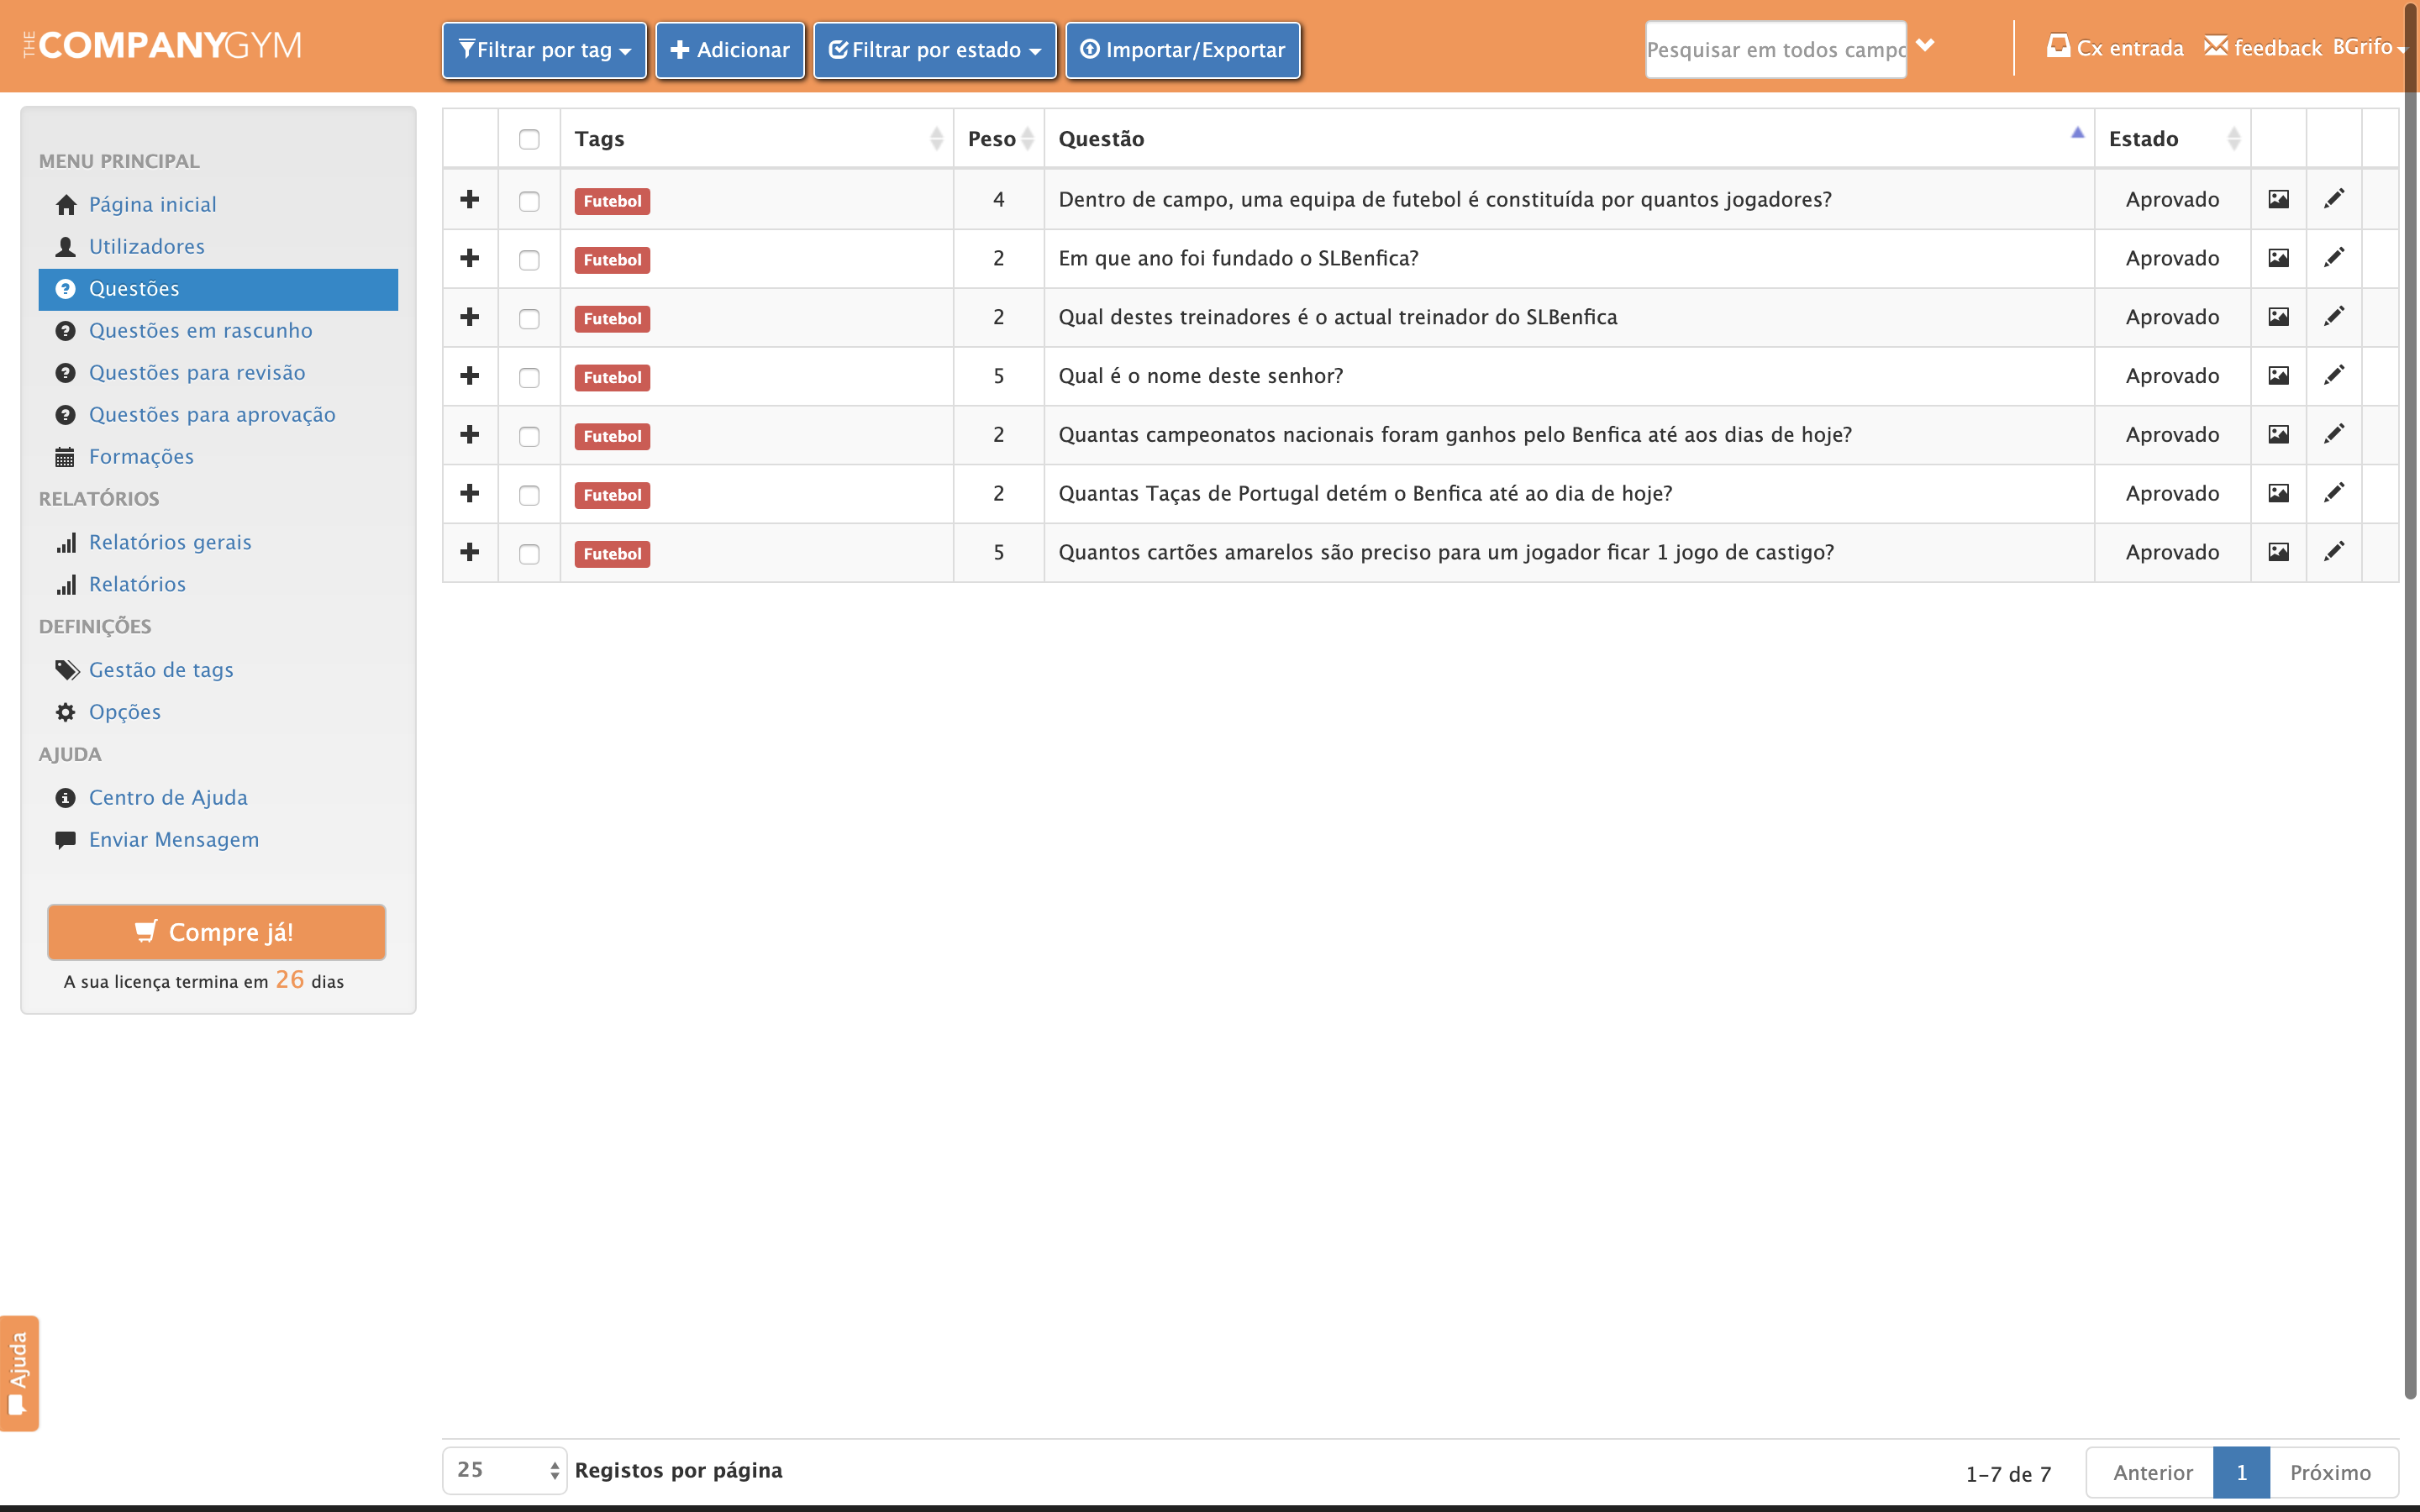
\includegraphics[width=1\textwidth]{img/tcg/tcg-questoes.png}
		\caption{The Company Gym - Lista de questões criadas}
		\label{fig:tcg-questoes}
	\end{center}
\end{figure}

\begin{figure}[ht!]
	\begin{center}
		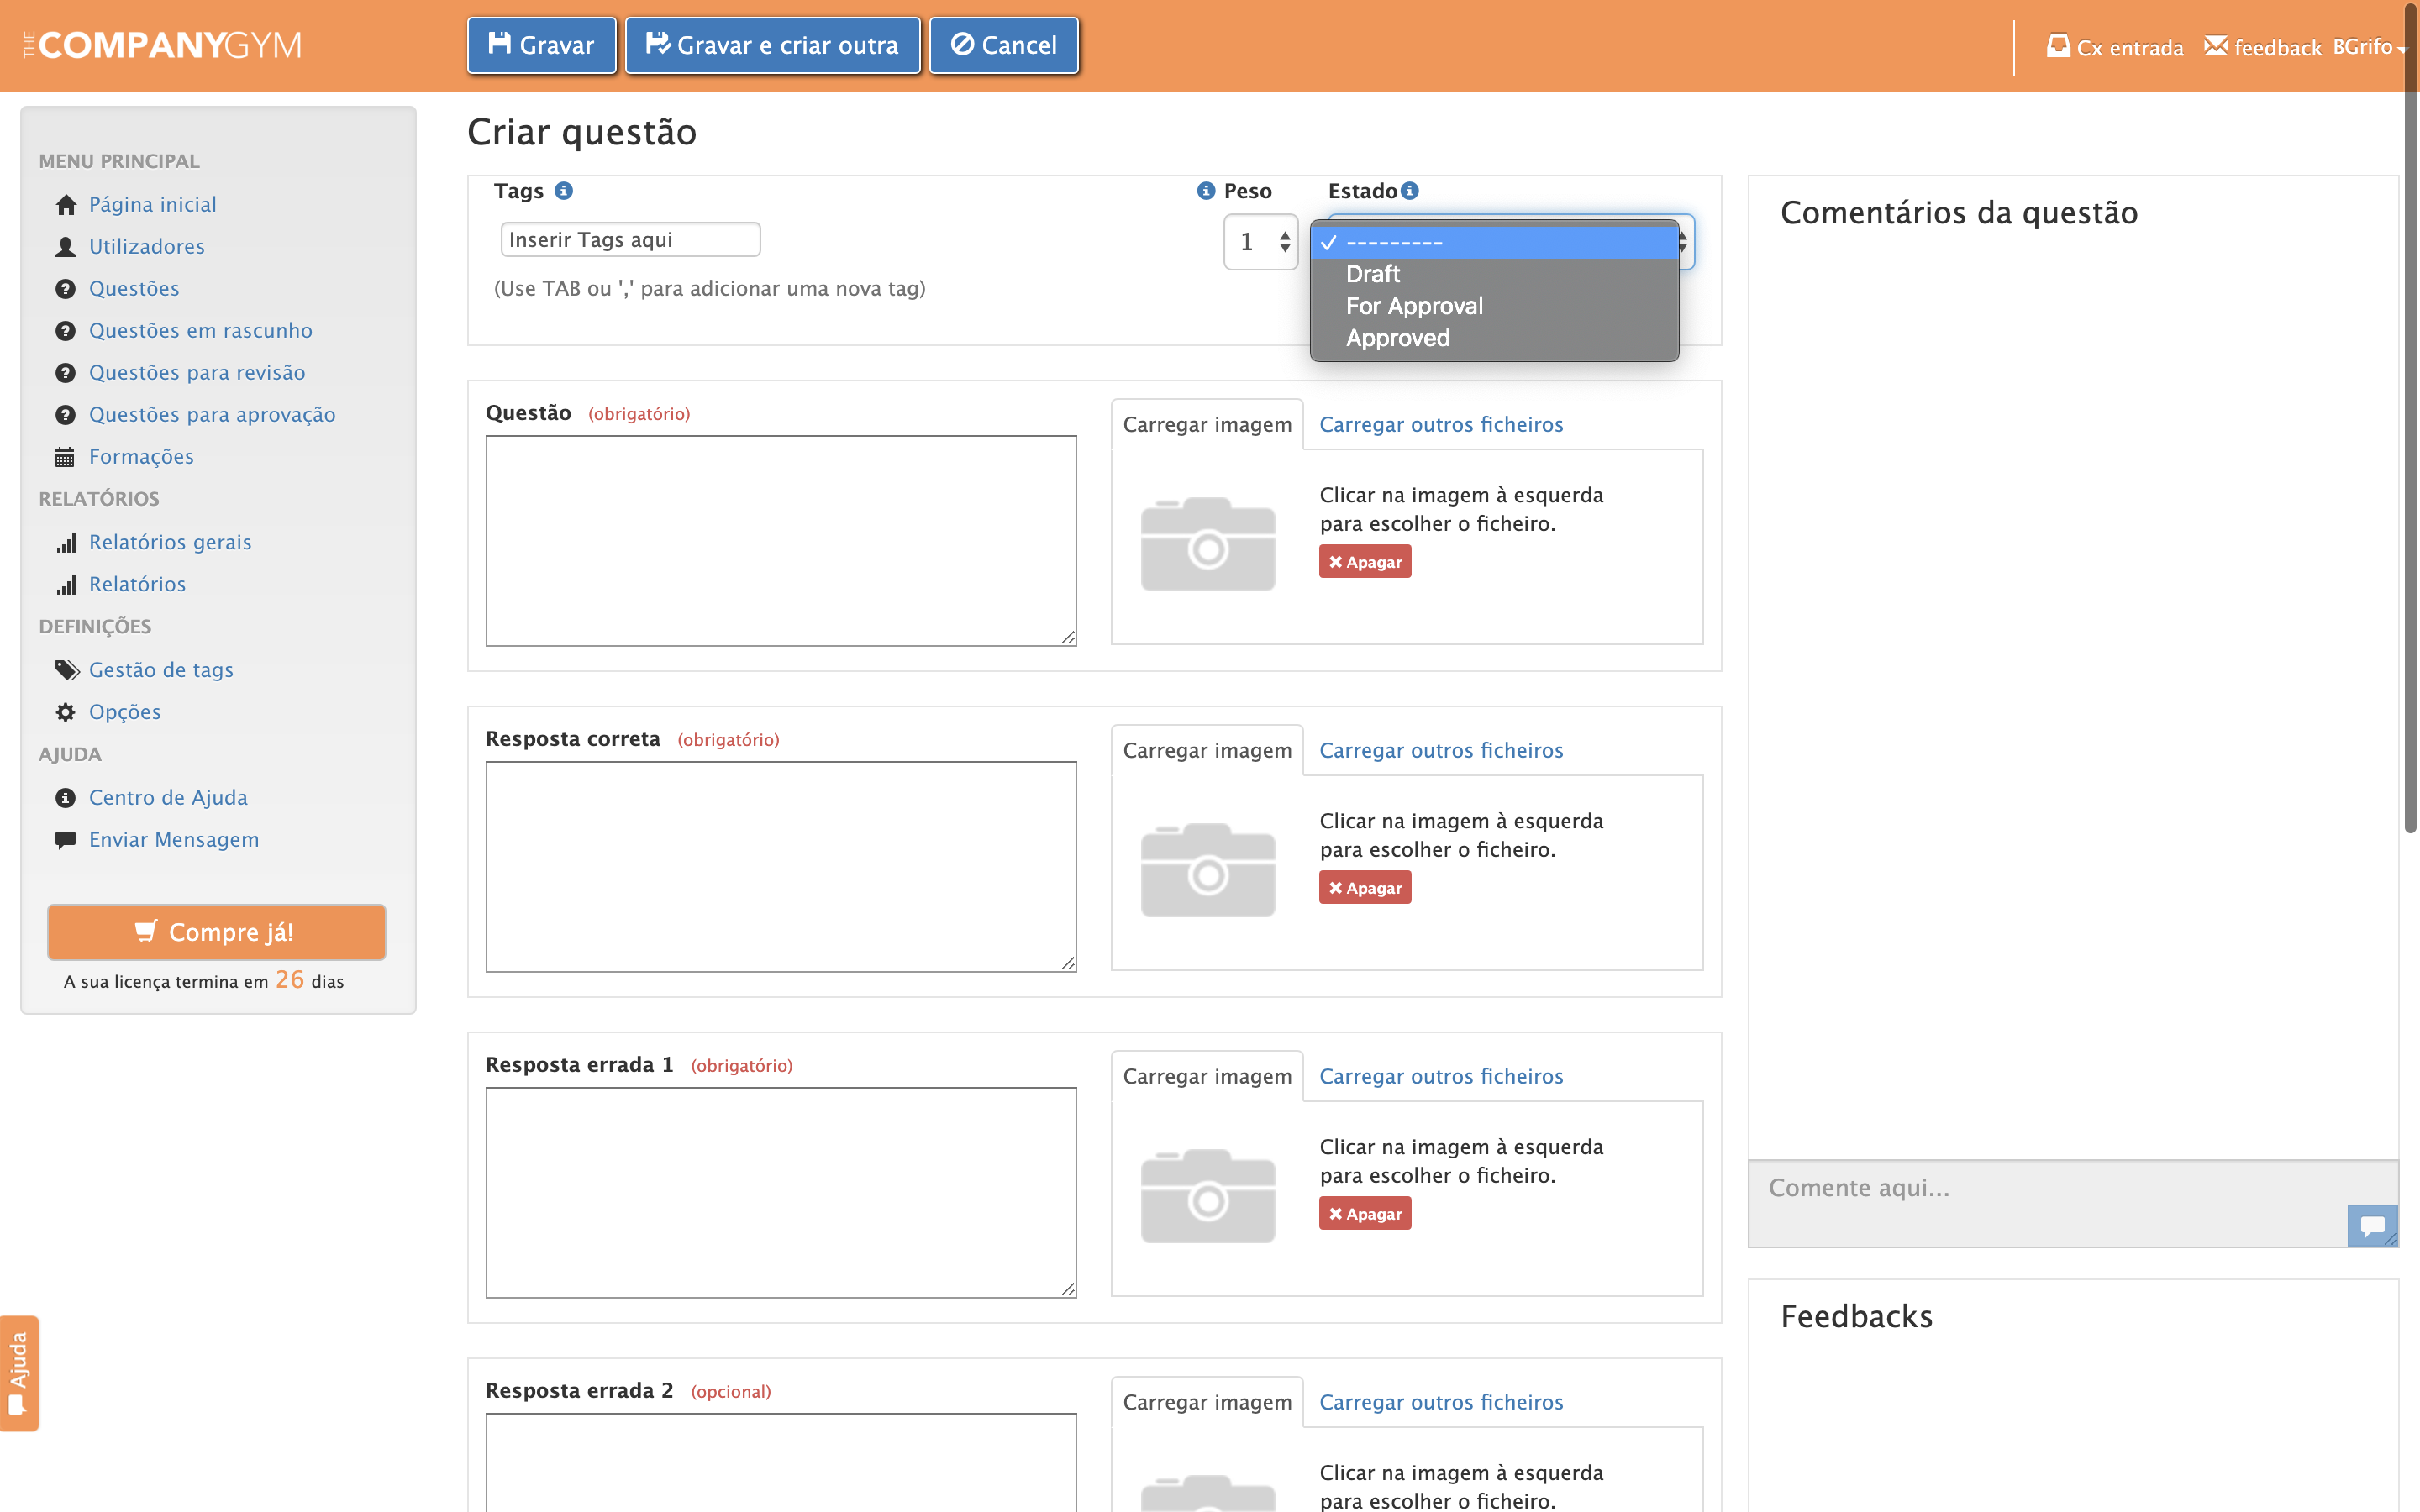
\includegraphics[width=1\textwidth]{img/tcg/tcg-criar-questao.png}
		\caption{The Company Gym - Criar questão}
		\label{fig:tcg-criar-questoes}
	\end{center}
\end{figure}

Na Figura \ref{fig:tcg-questoes} podemos ver que é possível listar todas as questões e filtrá-las por \textit{tags} e estado. À semelhança do que acontece com os utilizadores, é também possível importar e exportar questões. Como podemos ver na Figura \ref{fig:tcg-criar-questoes} para criar uma nova questão é necessário atribuir uma(s) \textit{tag}, um peso (i. e. importância), um estado (\textit{draft}, \textit{for approval} e \textit{approved}), a questão e pelo menos duas respostas. Alguns alpectos como o anexo (i. e. imagem, vídeo ou ficheiro de som) na pergunta e/ou resposta são opcionais. Quando se importa uma série de perguntas através de uma \textit{spreadsheet} todas as questões automaticamente ficam com estado \textit{draft} e como é de esperar sem anexos. Todas as questões que ficam em estado \textit{for approval} terão de ser aprovadas pelo gestor de conta.


Nas Figuras \ref{fig:tcg-form}, \ref{fig:tcg-form1} e \ref{fig:tcg-form2} temos todas as fases para a criação de uma formação. Em primeiro lugar, é necessário definir a periodicidade da formação.  Depois de escolher o nome é necessário dar um dia para o início e o fim da mesma, escolher os dias da semana em que o utilizador final irá receber a formação, a hora do dia a que recebe o mail e a duração (i. e. validade) que o utilizador tem para realizar a formação antes da mesma expirar. É de notar que a o sistema aceita uma duração com um máximo de horas igual à menor diferença entre os dias da semana escolhidos.

A seleção dos utilizadores finais e das questões faz-se através de tags. Desta forma temos uma forma bastante poderosa de adicionar múltiplas questões e ao mesmo tempo escolher exatamente quais as questões que queremos numa formação e sem ter que fazer quaisquer alterações, adicionar e remover questões a qualquer hora. O mesmo se trata para os utilizadores finais. 



\begin{figure}[ht!]
	\begin{center}
		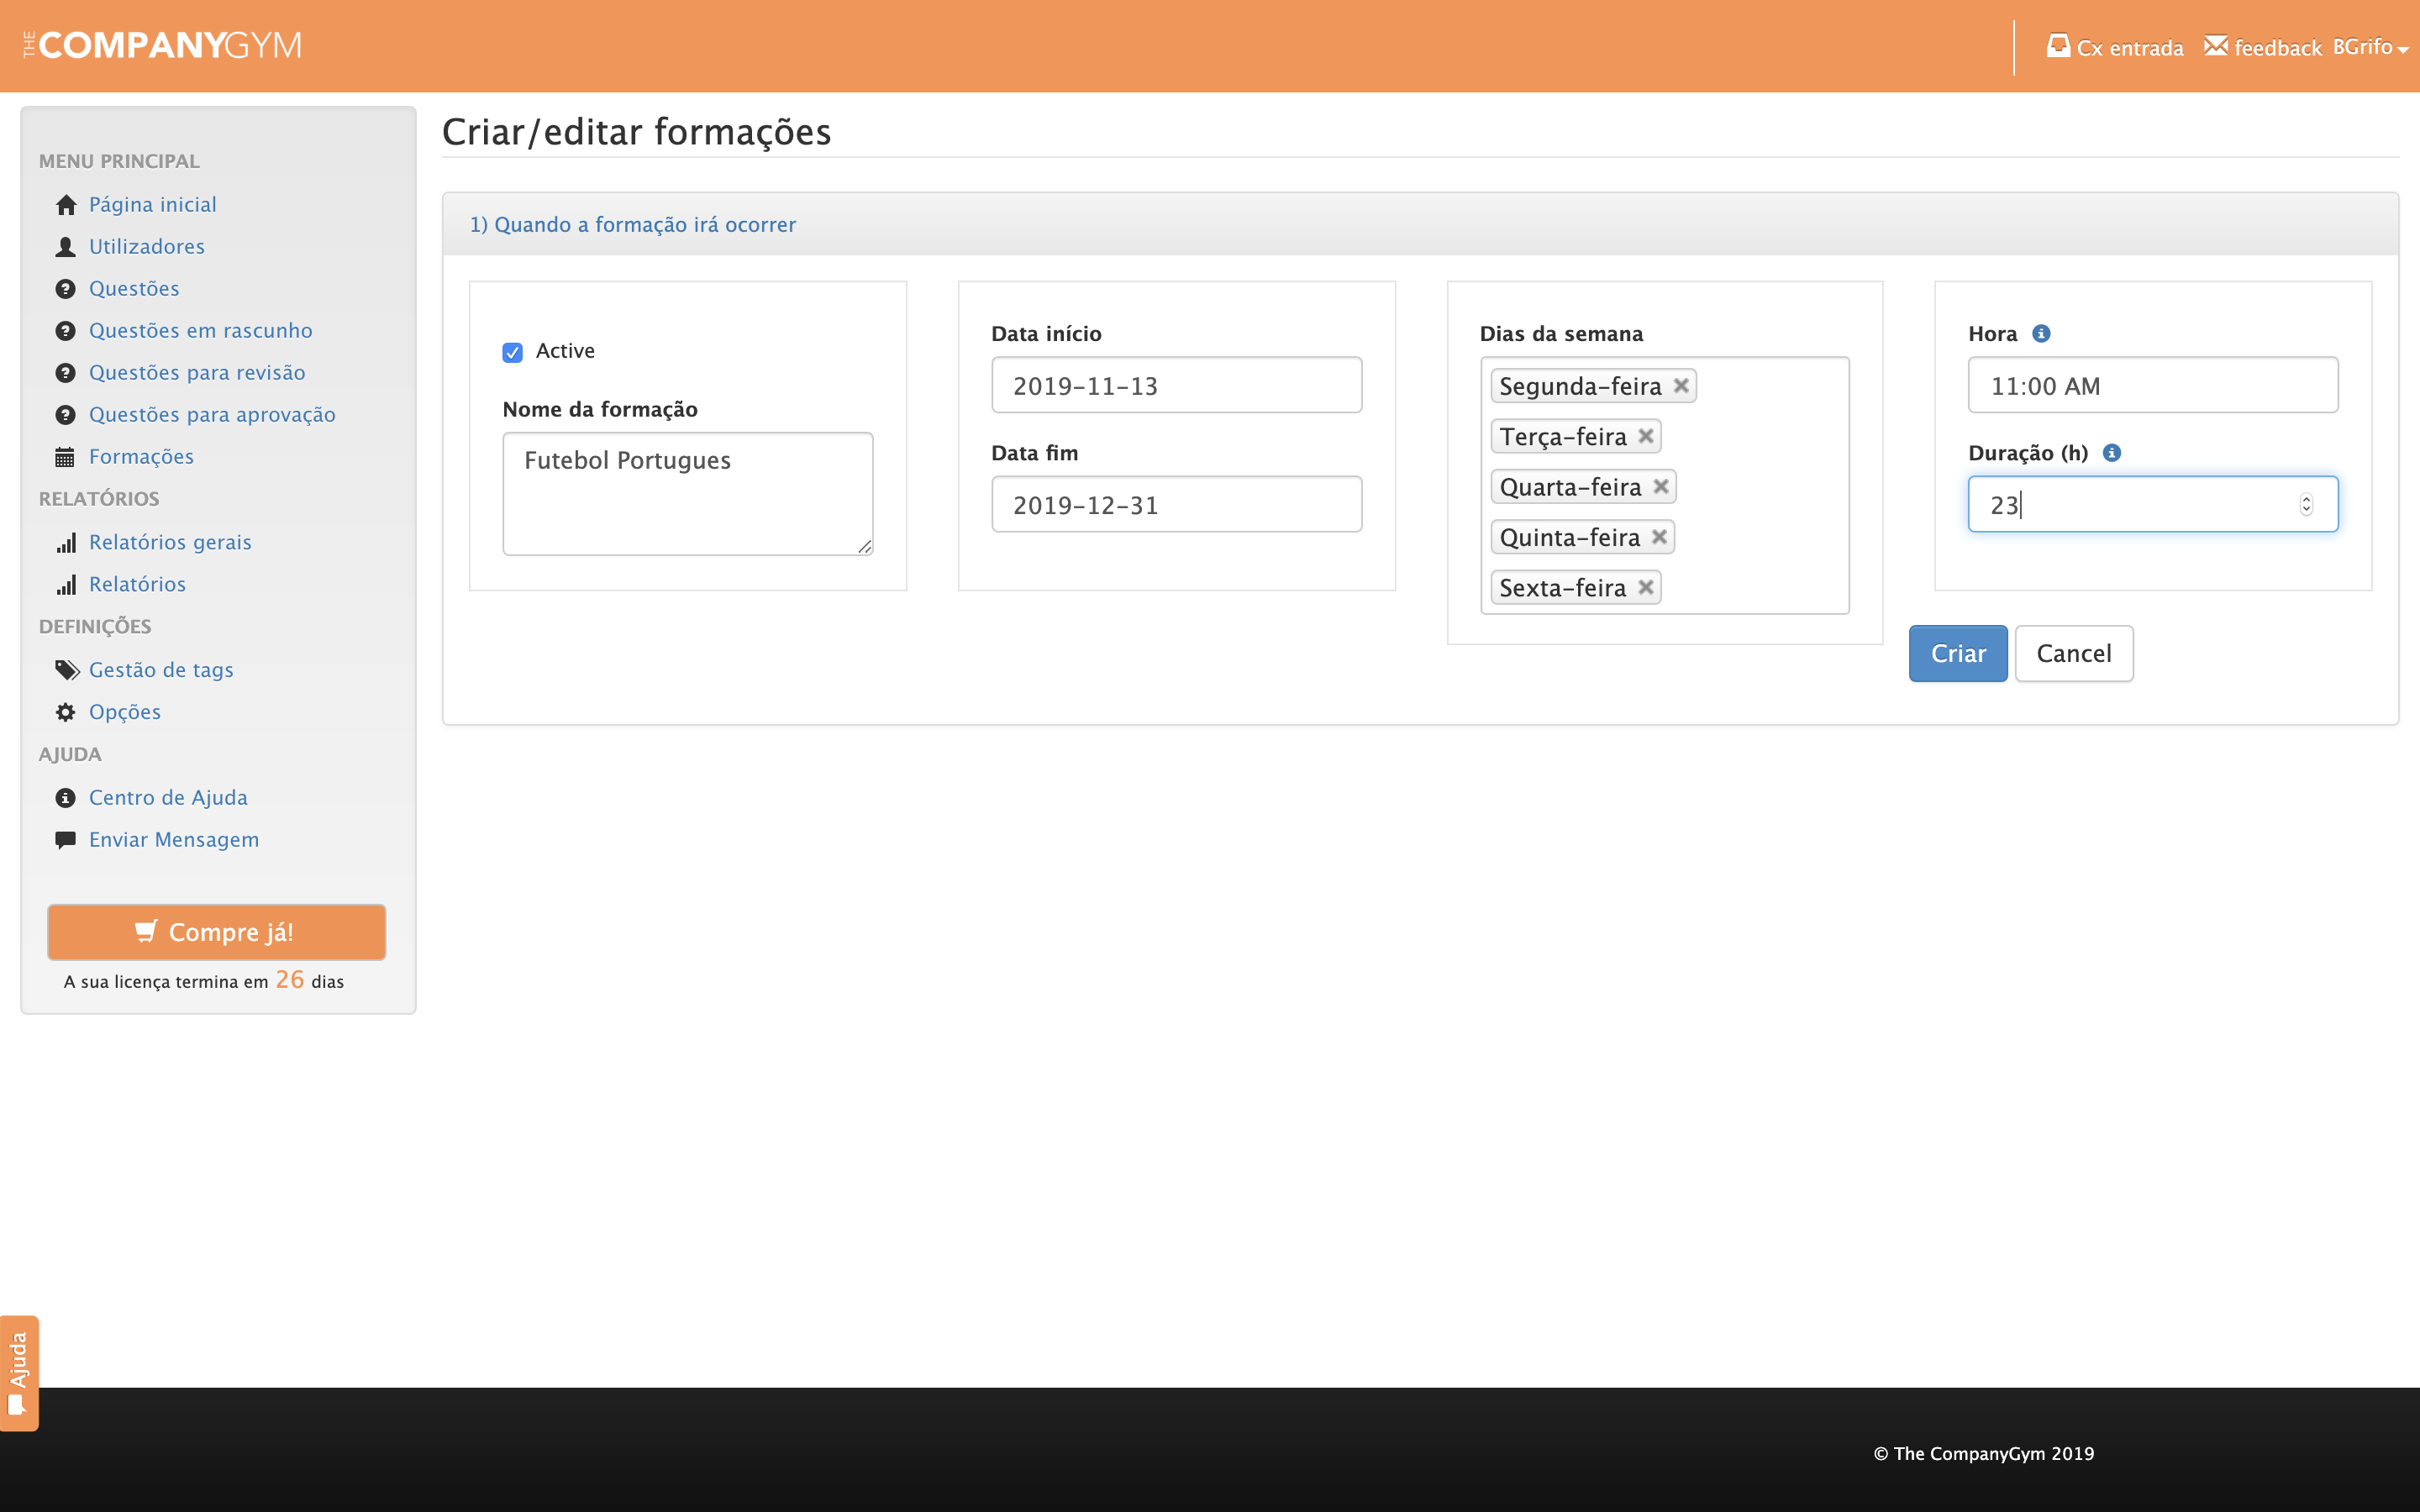
\includegraphics[width=1\textwidth]{img/tcg/tcg-form.png}
		\caption{The Company Gym - Criar Formação (Periodicidade)}
		\label{fig:tcg-form}
	\end{center}
\end{figure}

\newpage


\begin{figure}[ht!]
	\begin{center}
		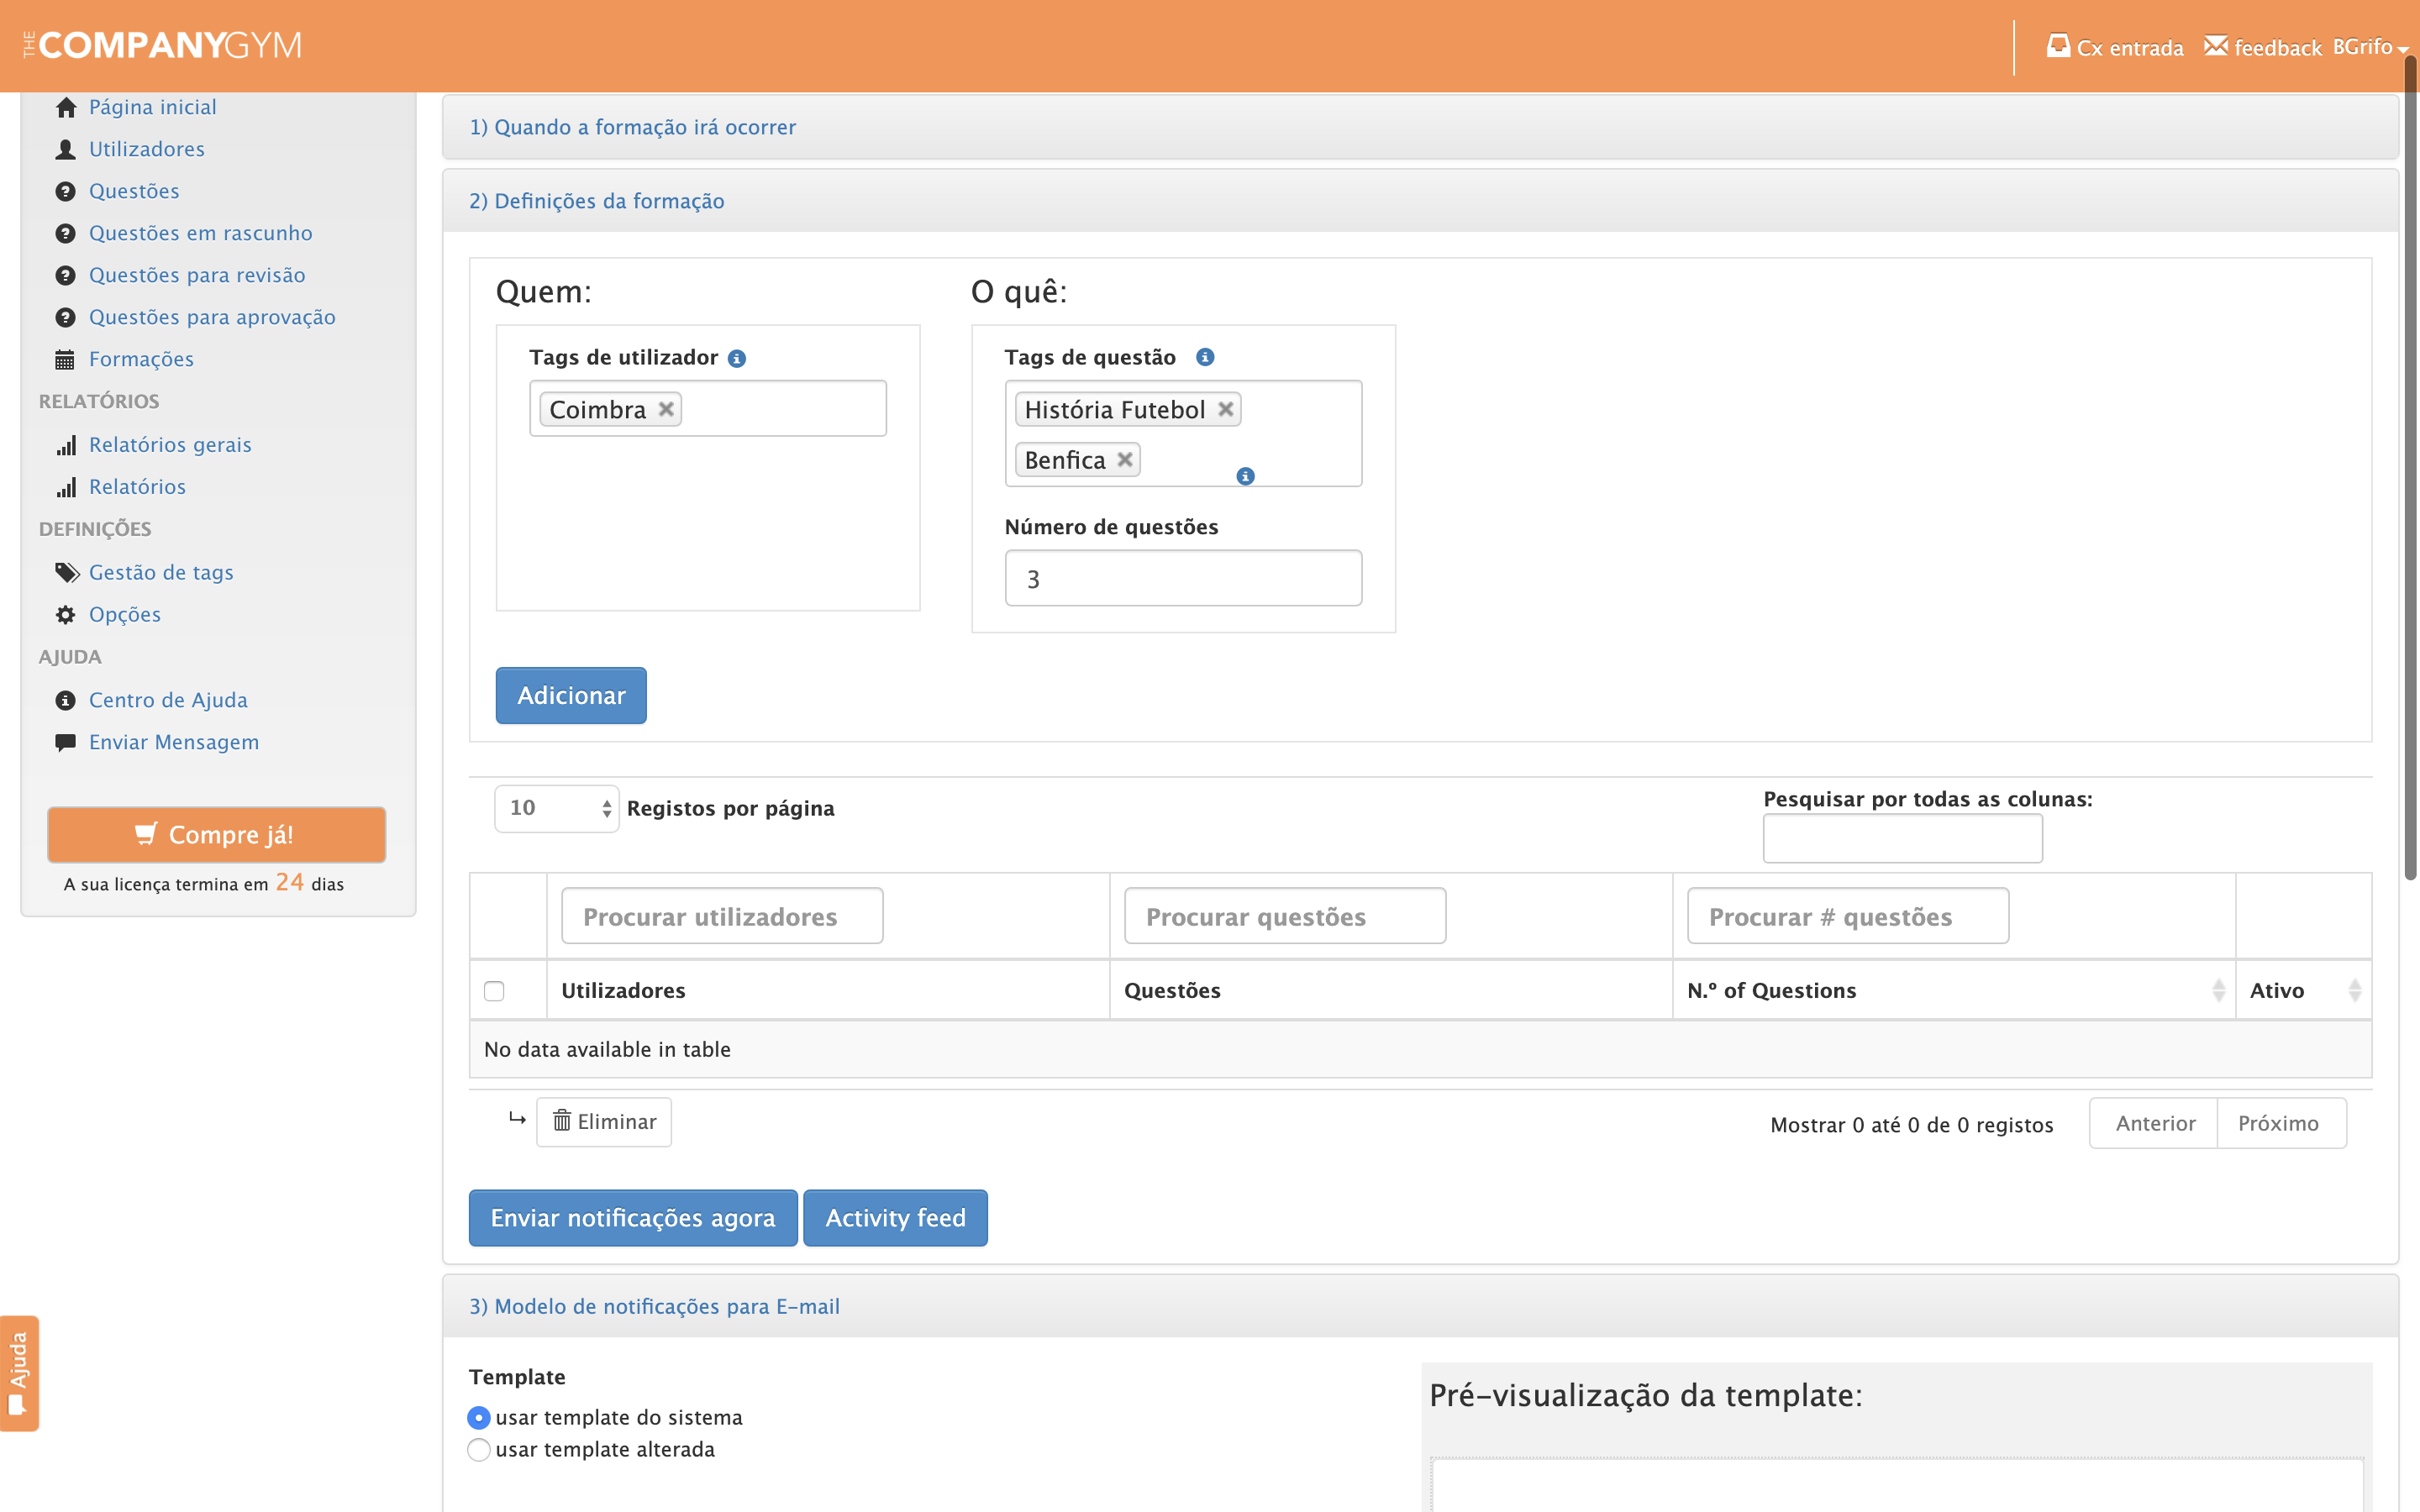
\includegraphics[width=1\textwidth]{img/tcg/tcg-form1.png}
		\caption{The Company Gym - Criar Formação (Definições)}
		\label{fig:tcg-form1}
	\end{center}
\end{figure}

\begin{figure}[ht!]
	\begin{center}
		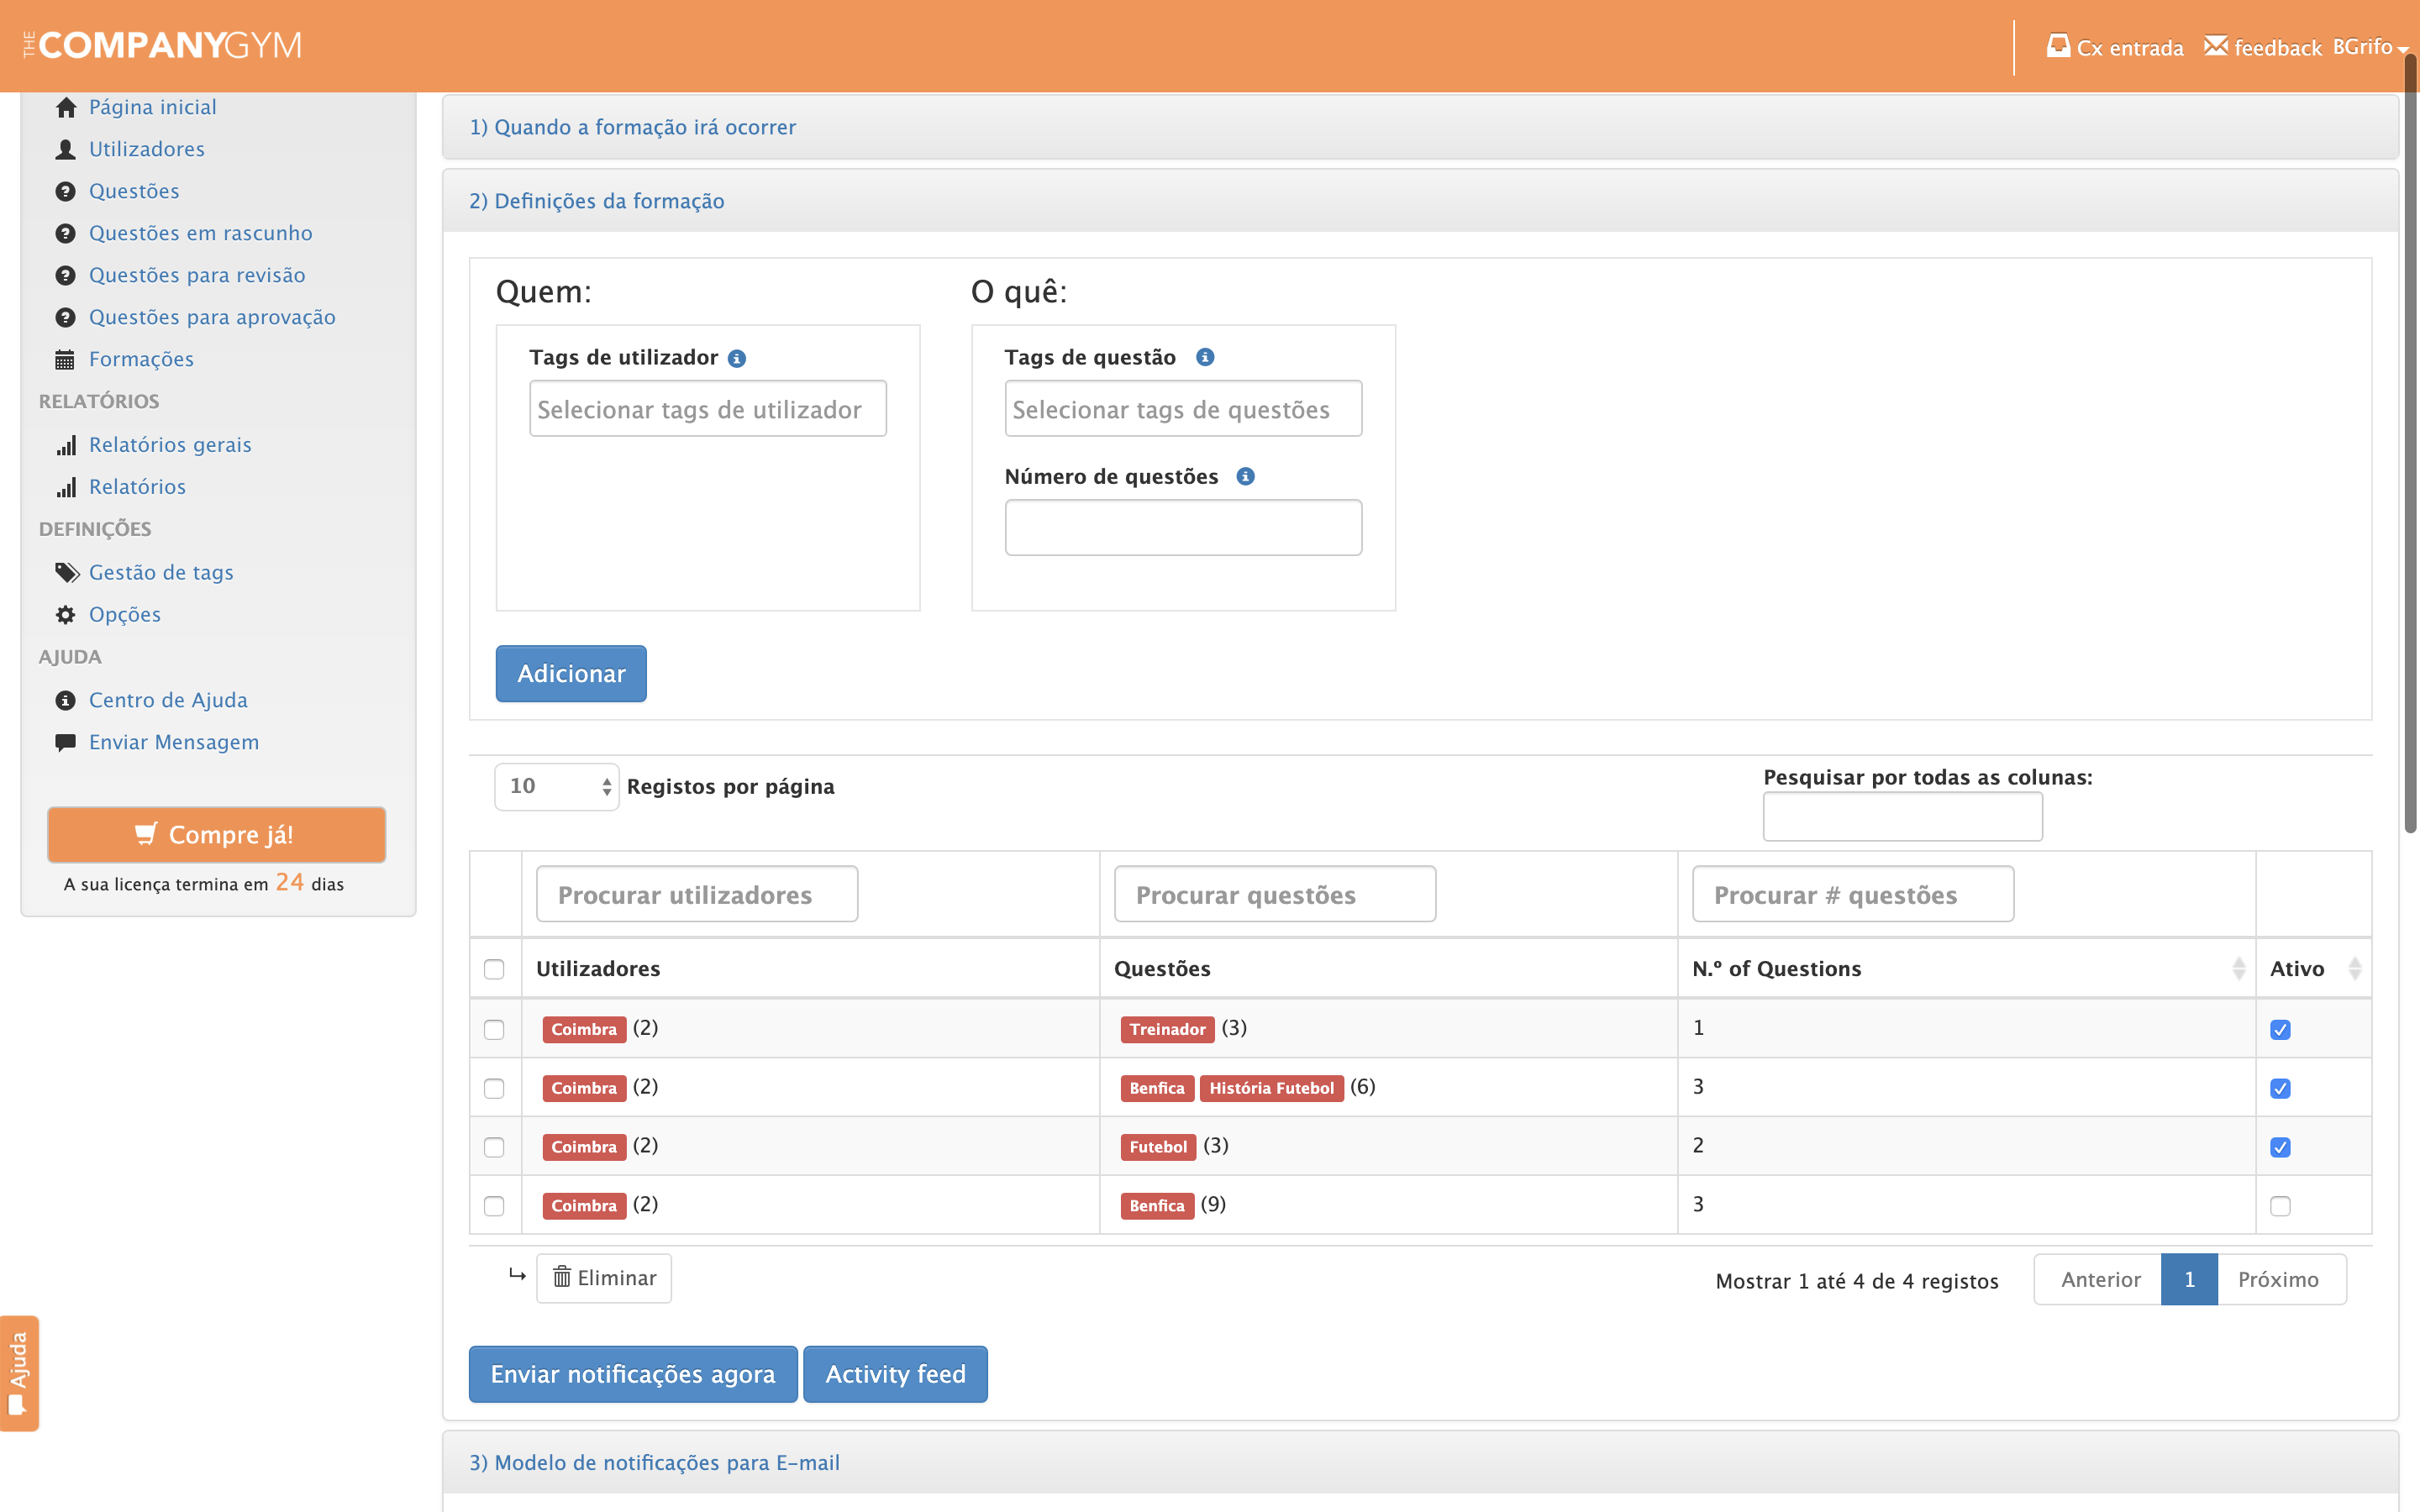
\includegraphics[width=1\textwidth]{img/tcg/tcg-form2.png}
		\caption{The Company Gym - Criar Formação (Gerir Utilizadores e Questões)}
		\label{fig:tcg-form2}
	\end{center}
\end{figure}

O botão "Activity feed" abre uma nova janela com o histórico de actividades da formação como podemos ver na Figura \ref{fig:tcg-feed}. O histórico pode ser organizado pelas caracteristica de cada coluna e para cada registo, é possível ver verificar as respostas do utilizador final na formação.


\begin{figure}[ht!]
	\begin{center}
		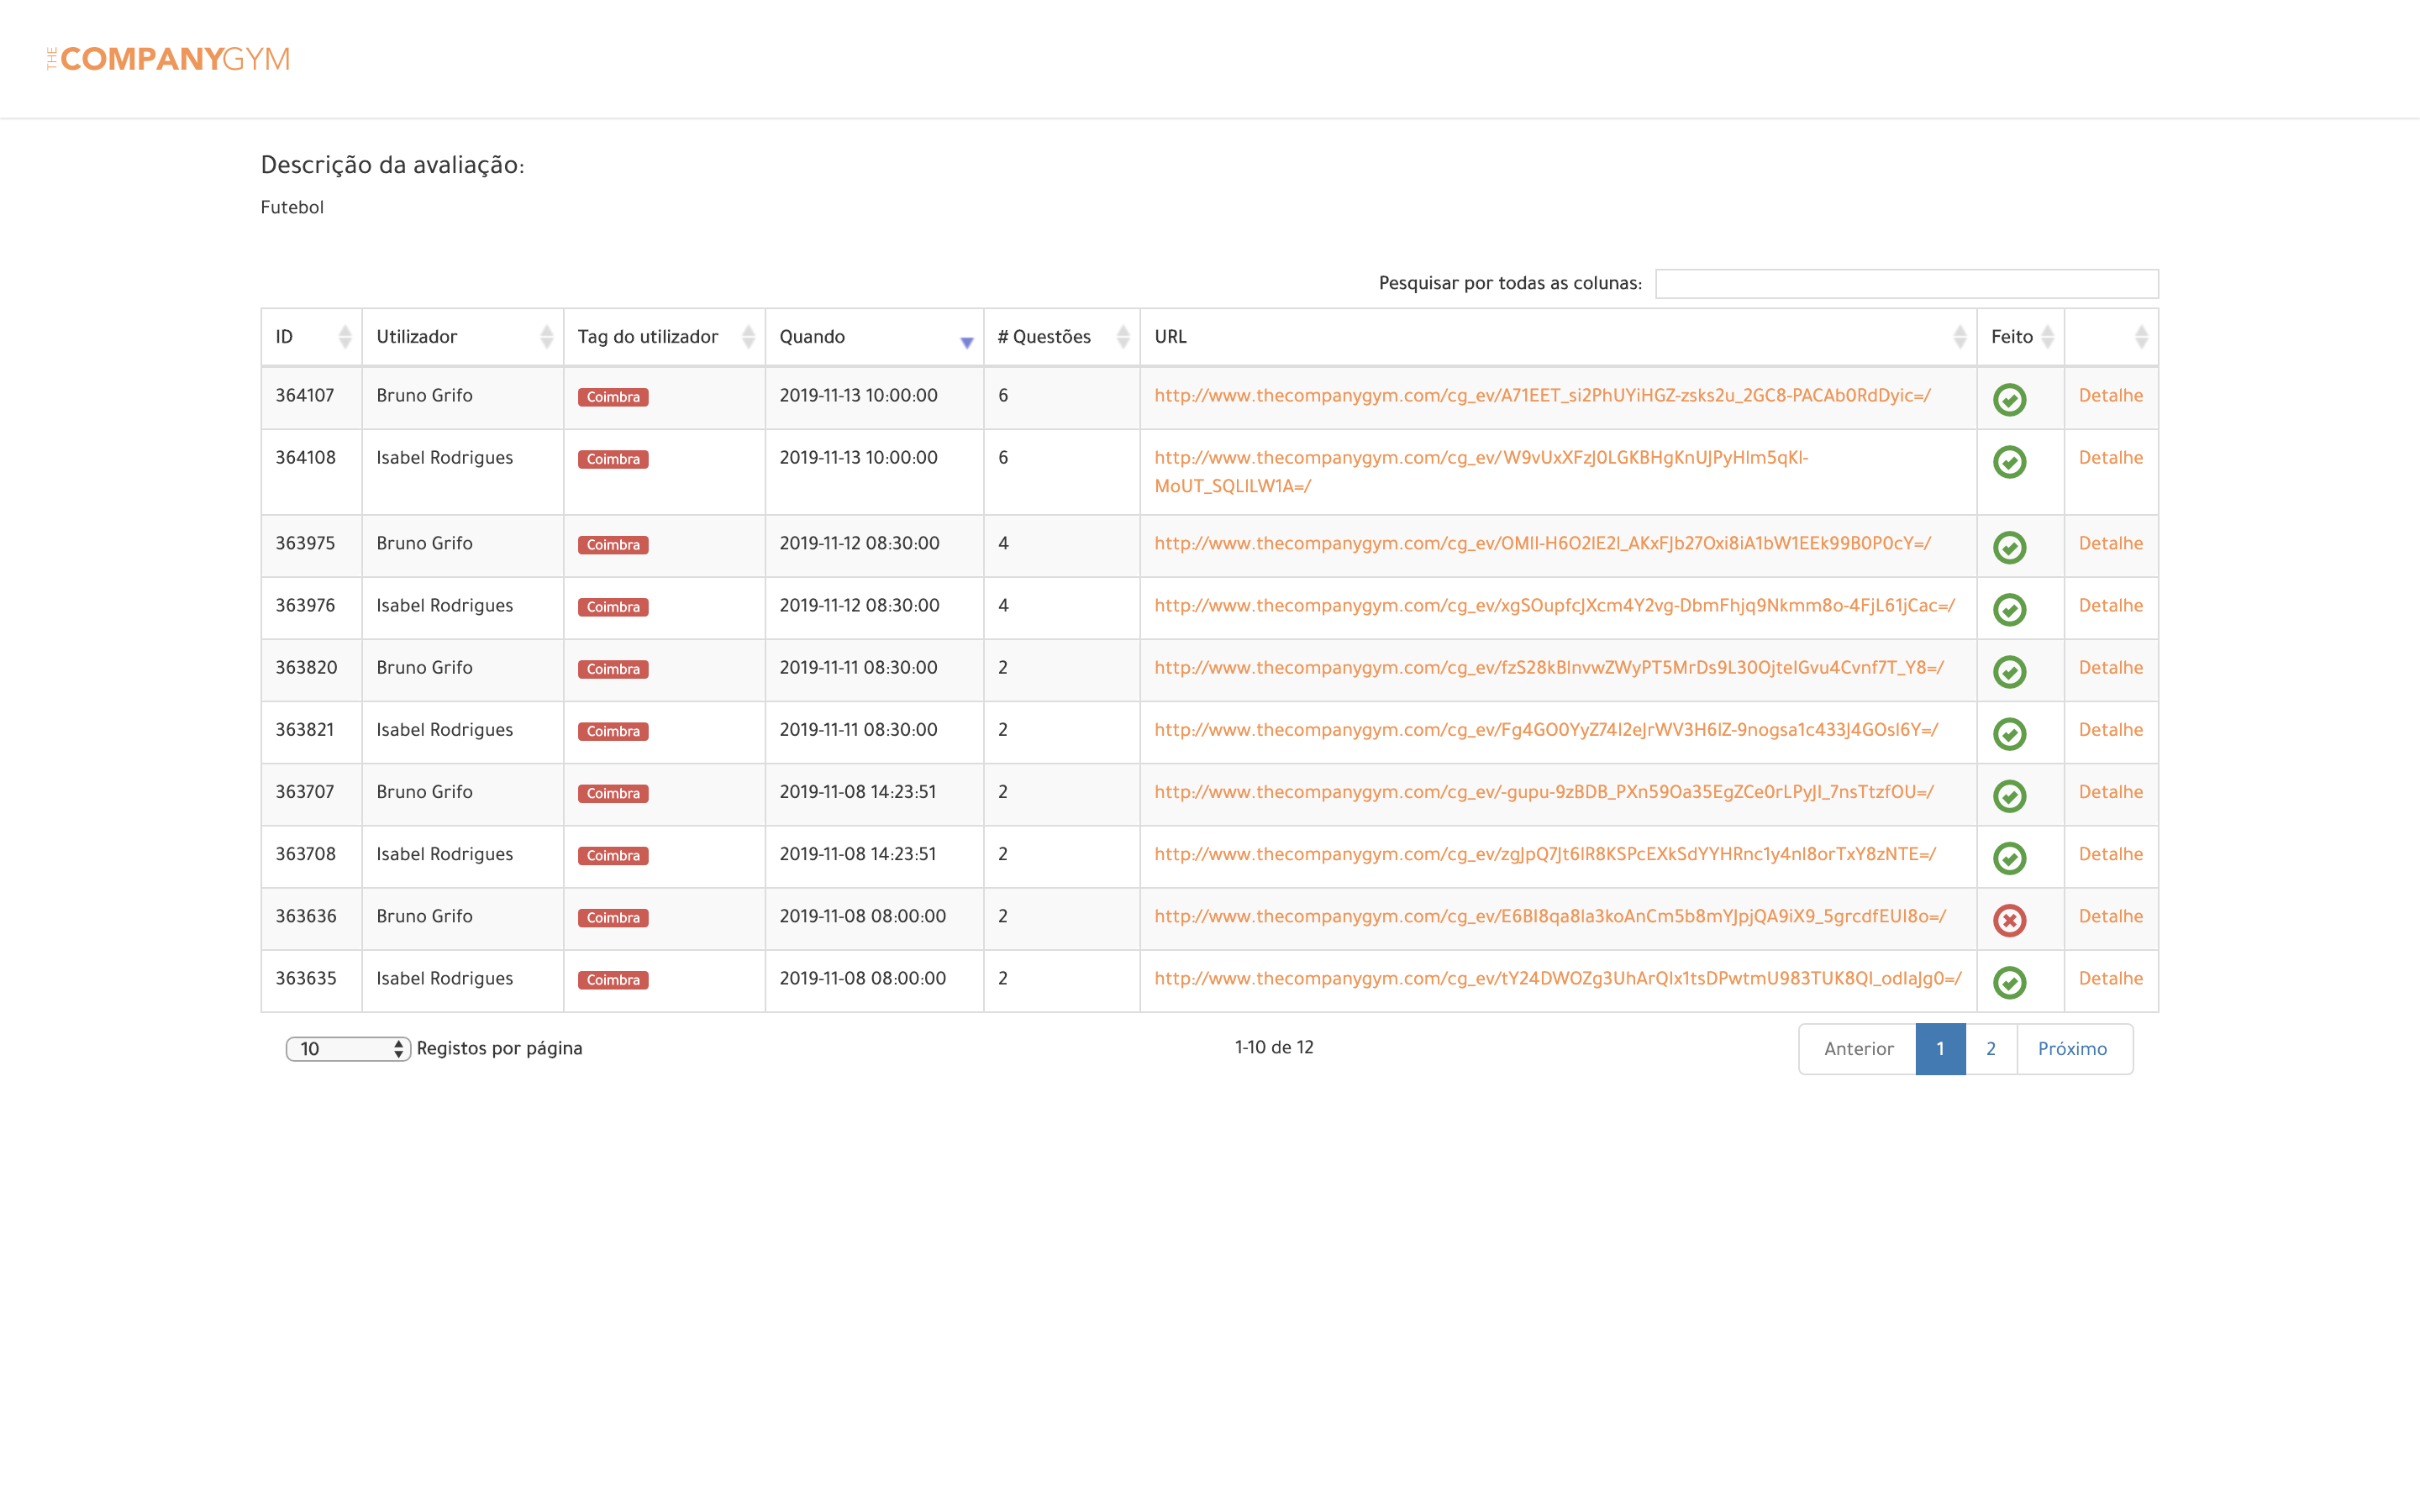
\includegraphics[width=1\textwidth]{img/tcg/tcg-feed.png}
		\caption{The Company Gym - Histórico de actividades}
		\label{fig:tcg-feed}
	\end{center}
\end{figure}

\newpage


\begin{figure}[ht!]
	\begin{center}
		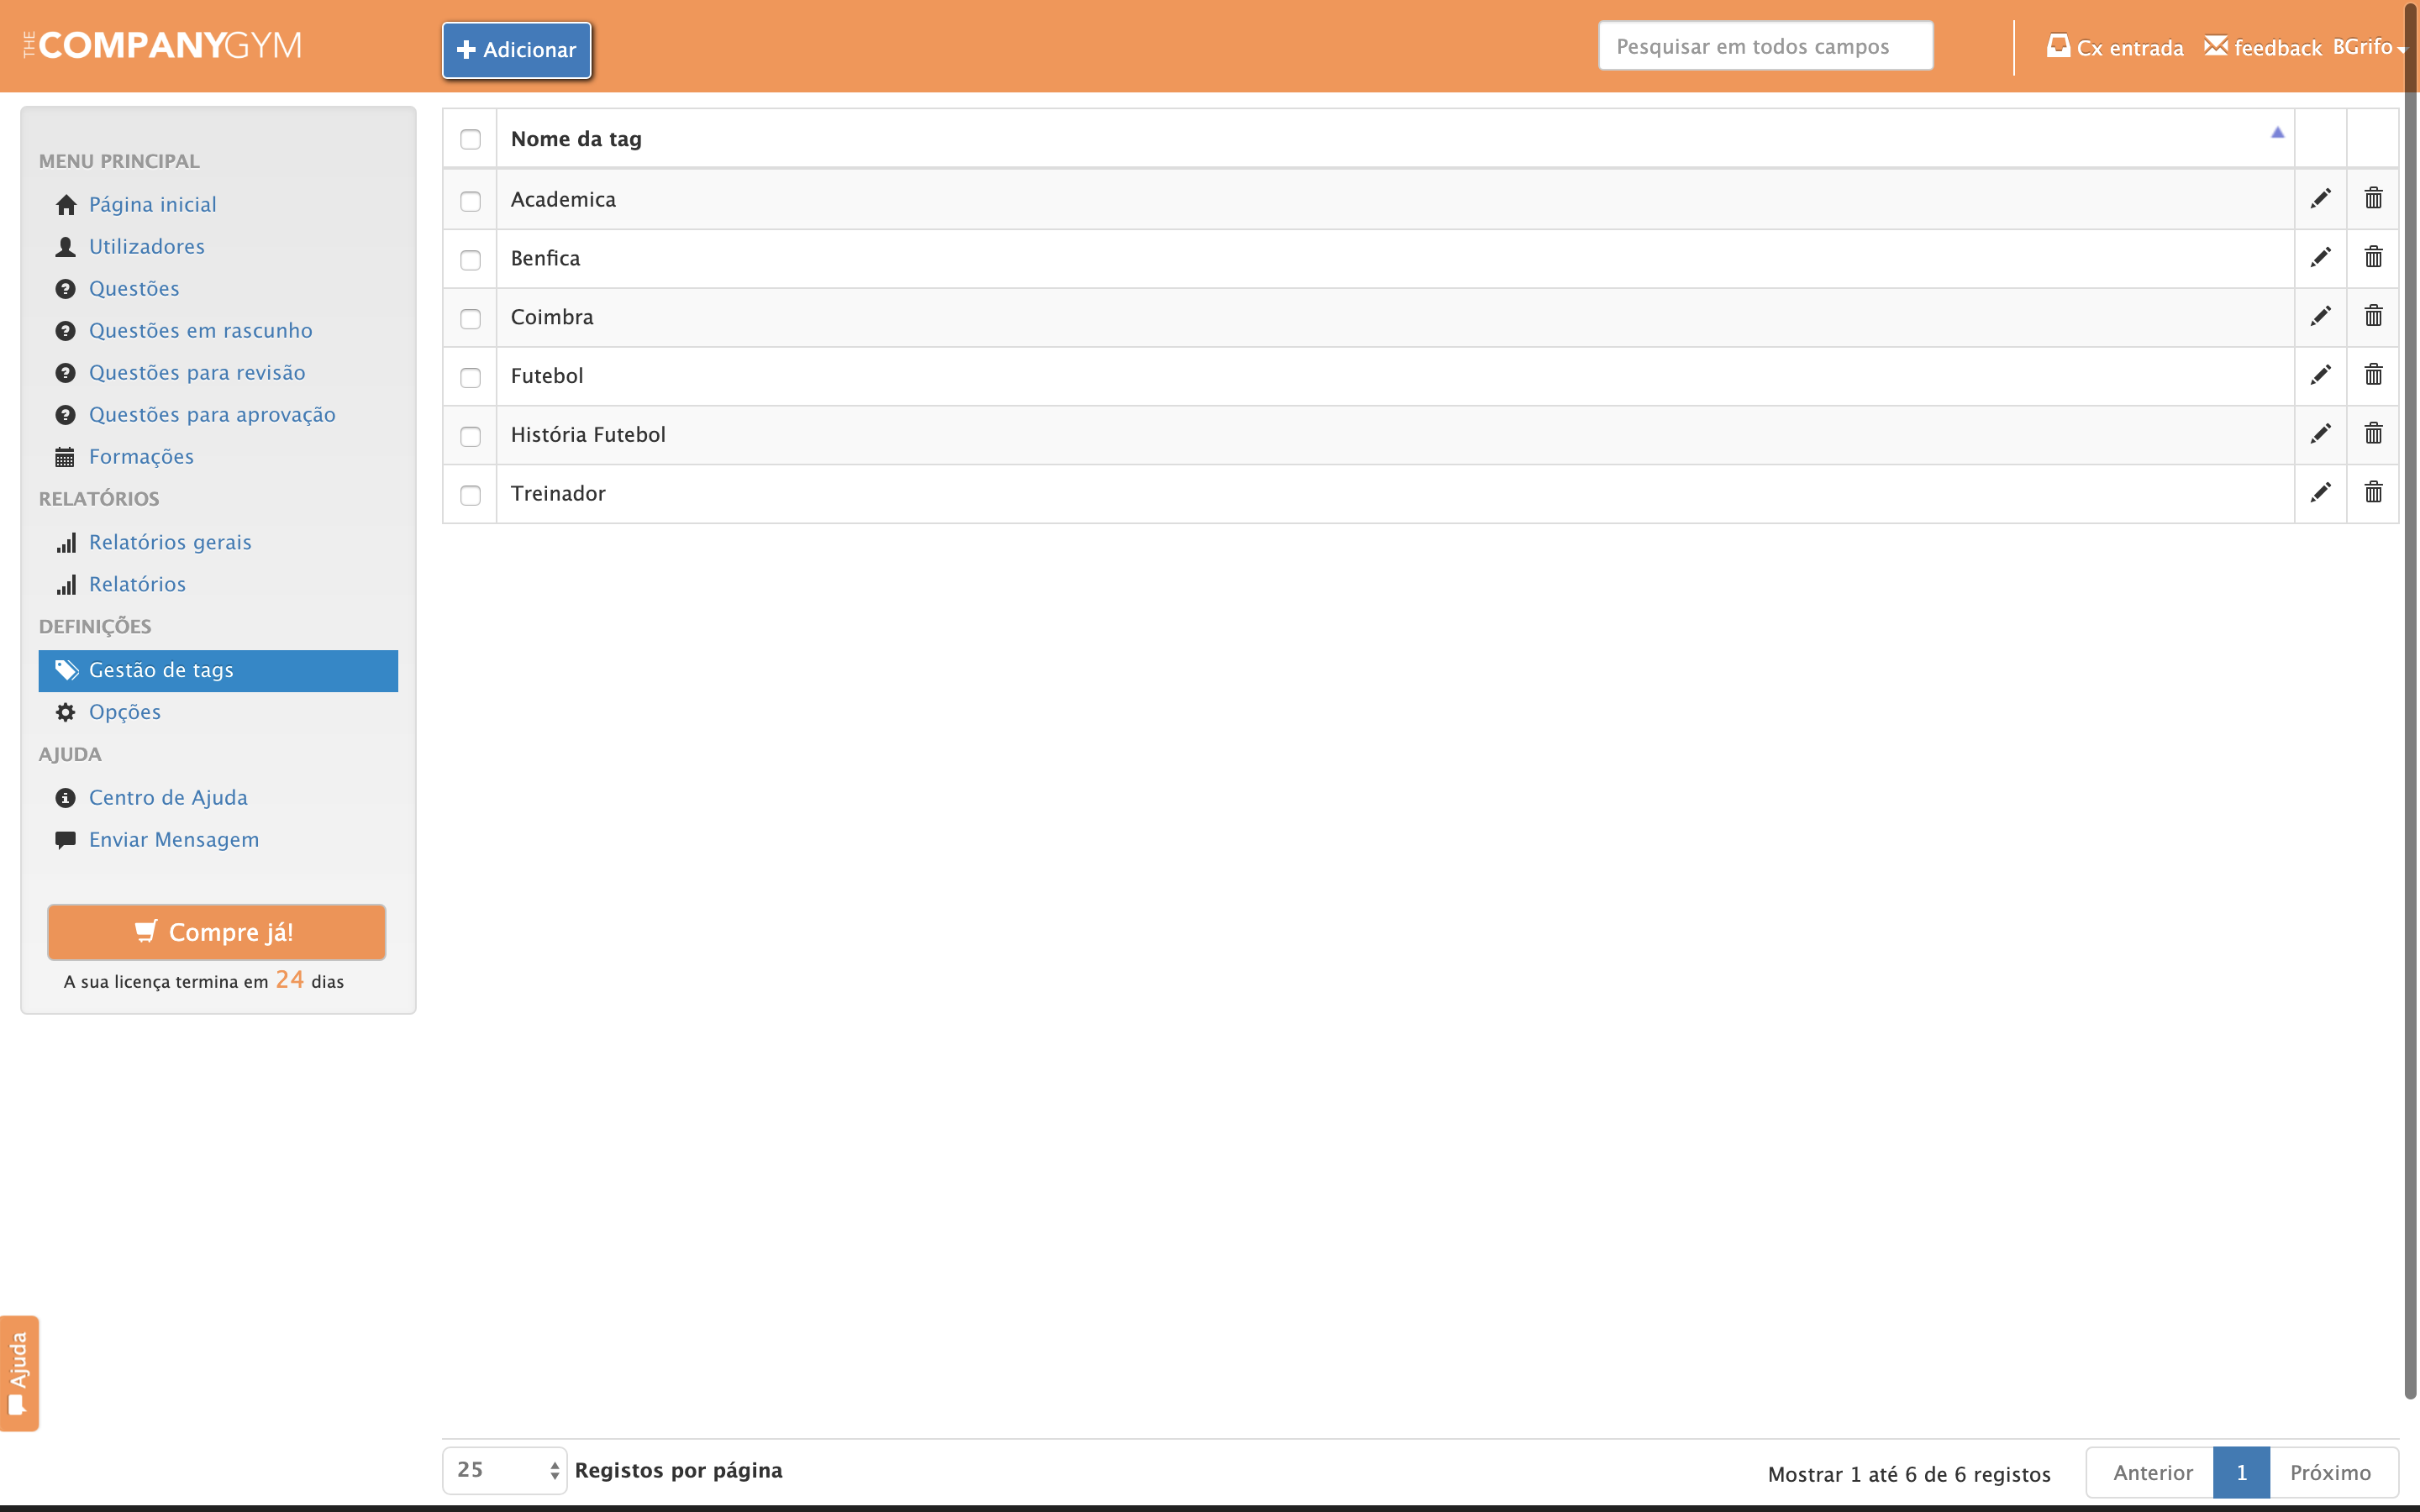
\includegraphics[width=1\textwidth]{img/tcg/tcg-tags.png}
		\caption{The Company Gym - Lista de Tags}
		\label{fig:tcg-tags}
	\end{center}
\end{figure}

É também possível gerir todas as Tags (i. e. adicionar, editar e remover) adicionadas pelo utilizador no sistema como podemos ver na Figura \ref{fig:tcg-tags} e alterar o template do mail que é enviado para os clientes finais com o link para a formação, representado na Figura \ref{fig:tcg-mail}. 

\begin{figure}[ht!]
	\begin{center}
		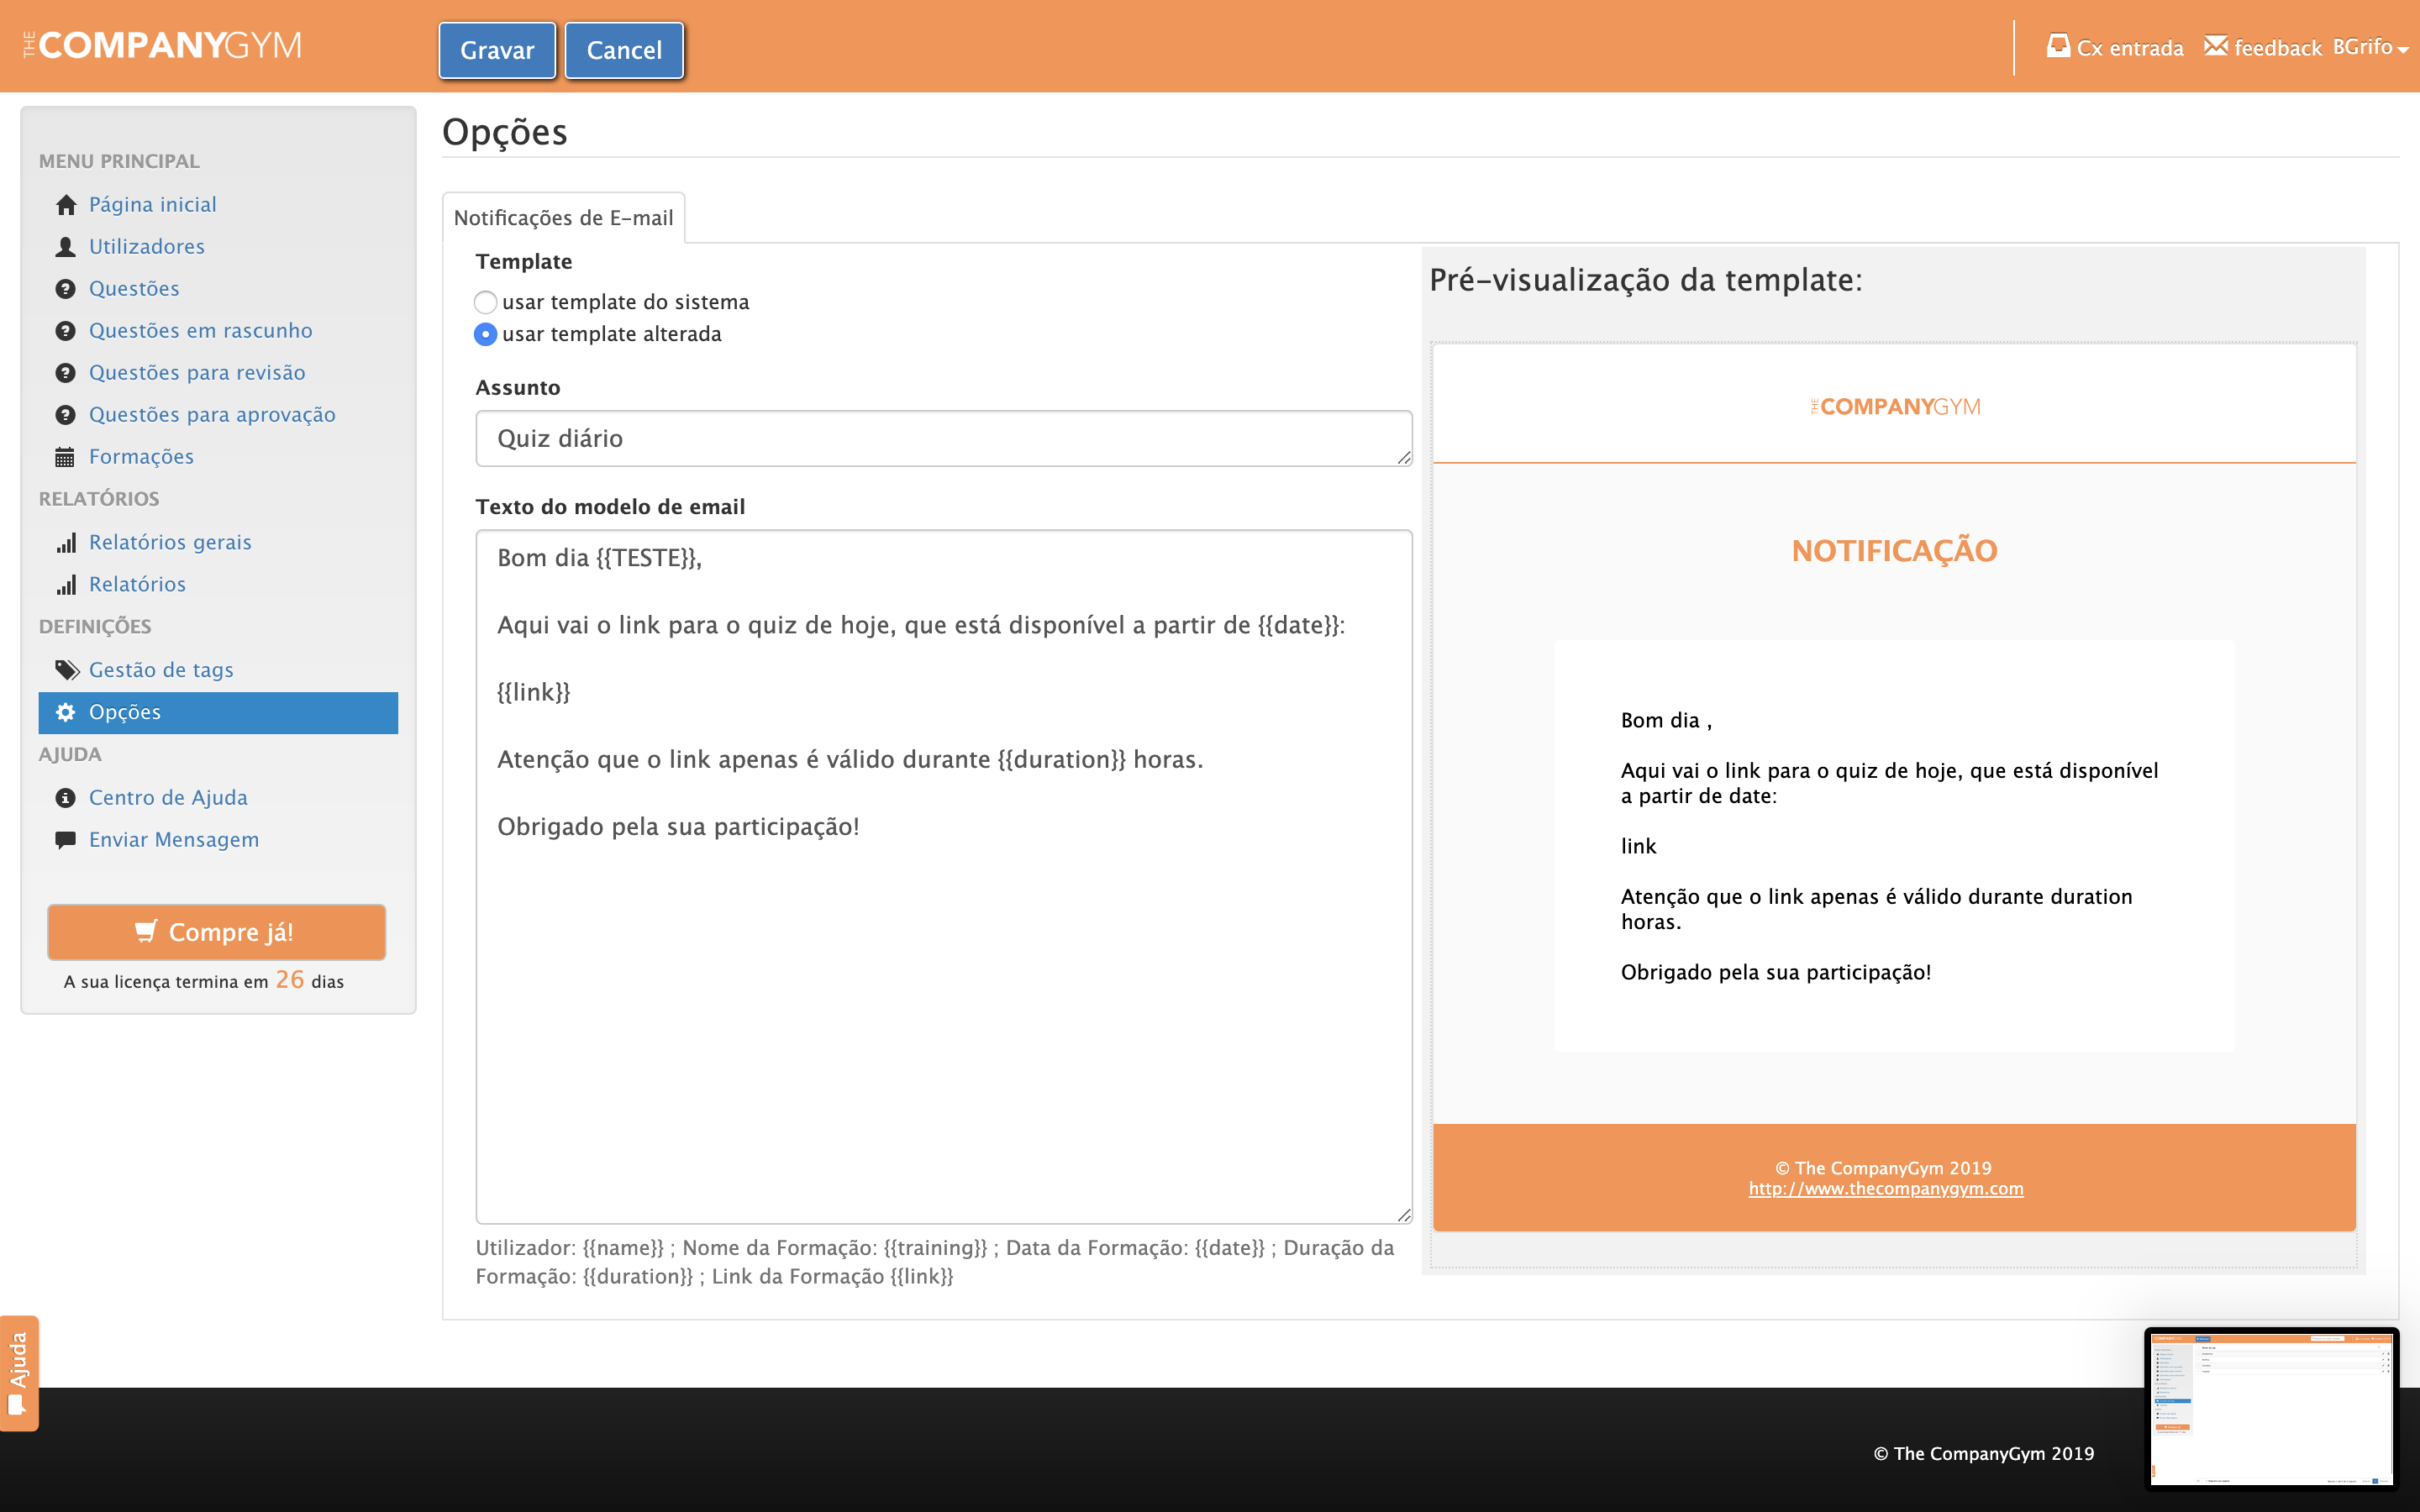
\includegraphics[width=1\textwidth]{img/tcg/tcg-mail.png}
		\caption{The Company Gym - Alterar template do mail}
		\label{fig:tcg-mail}
	\end{center}
\end{figure}

\newpage

Na análise de resultados, podemos gerar relatórios gerais (i. e. relatórios com estatísticas de todas as formações, questões e utilizadores), como podemos ver na Figura \ref{fig:tcg-data}  e relatórios para uma formação em específico (i. e. relatórios com estatísticas apenas das formações, questões e utilizadores adicionados a essa formação). 

\begin{figure}[ht!]
	\begin{center}
		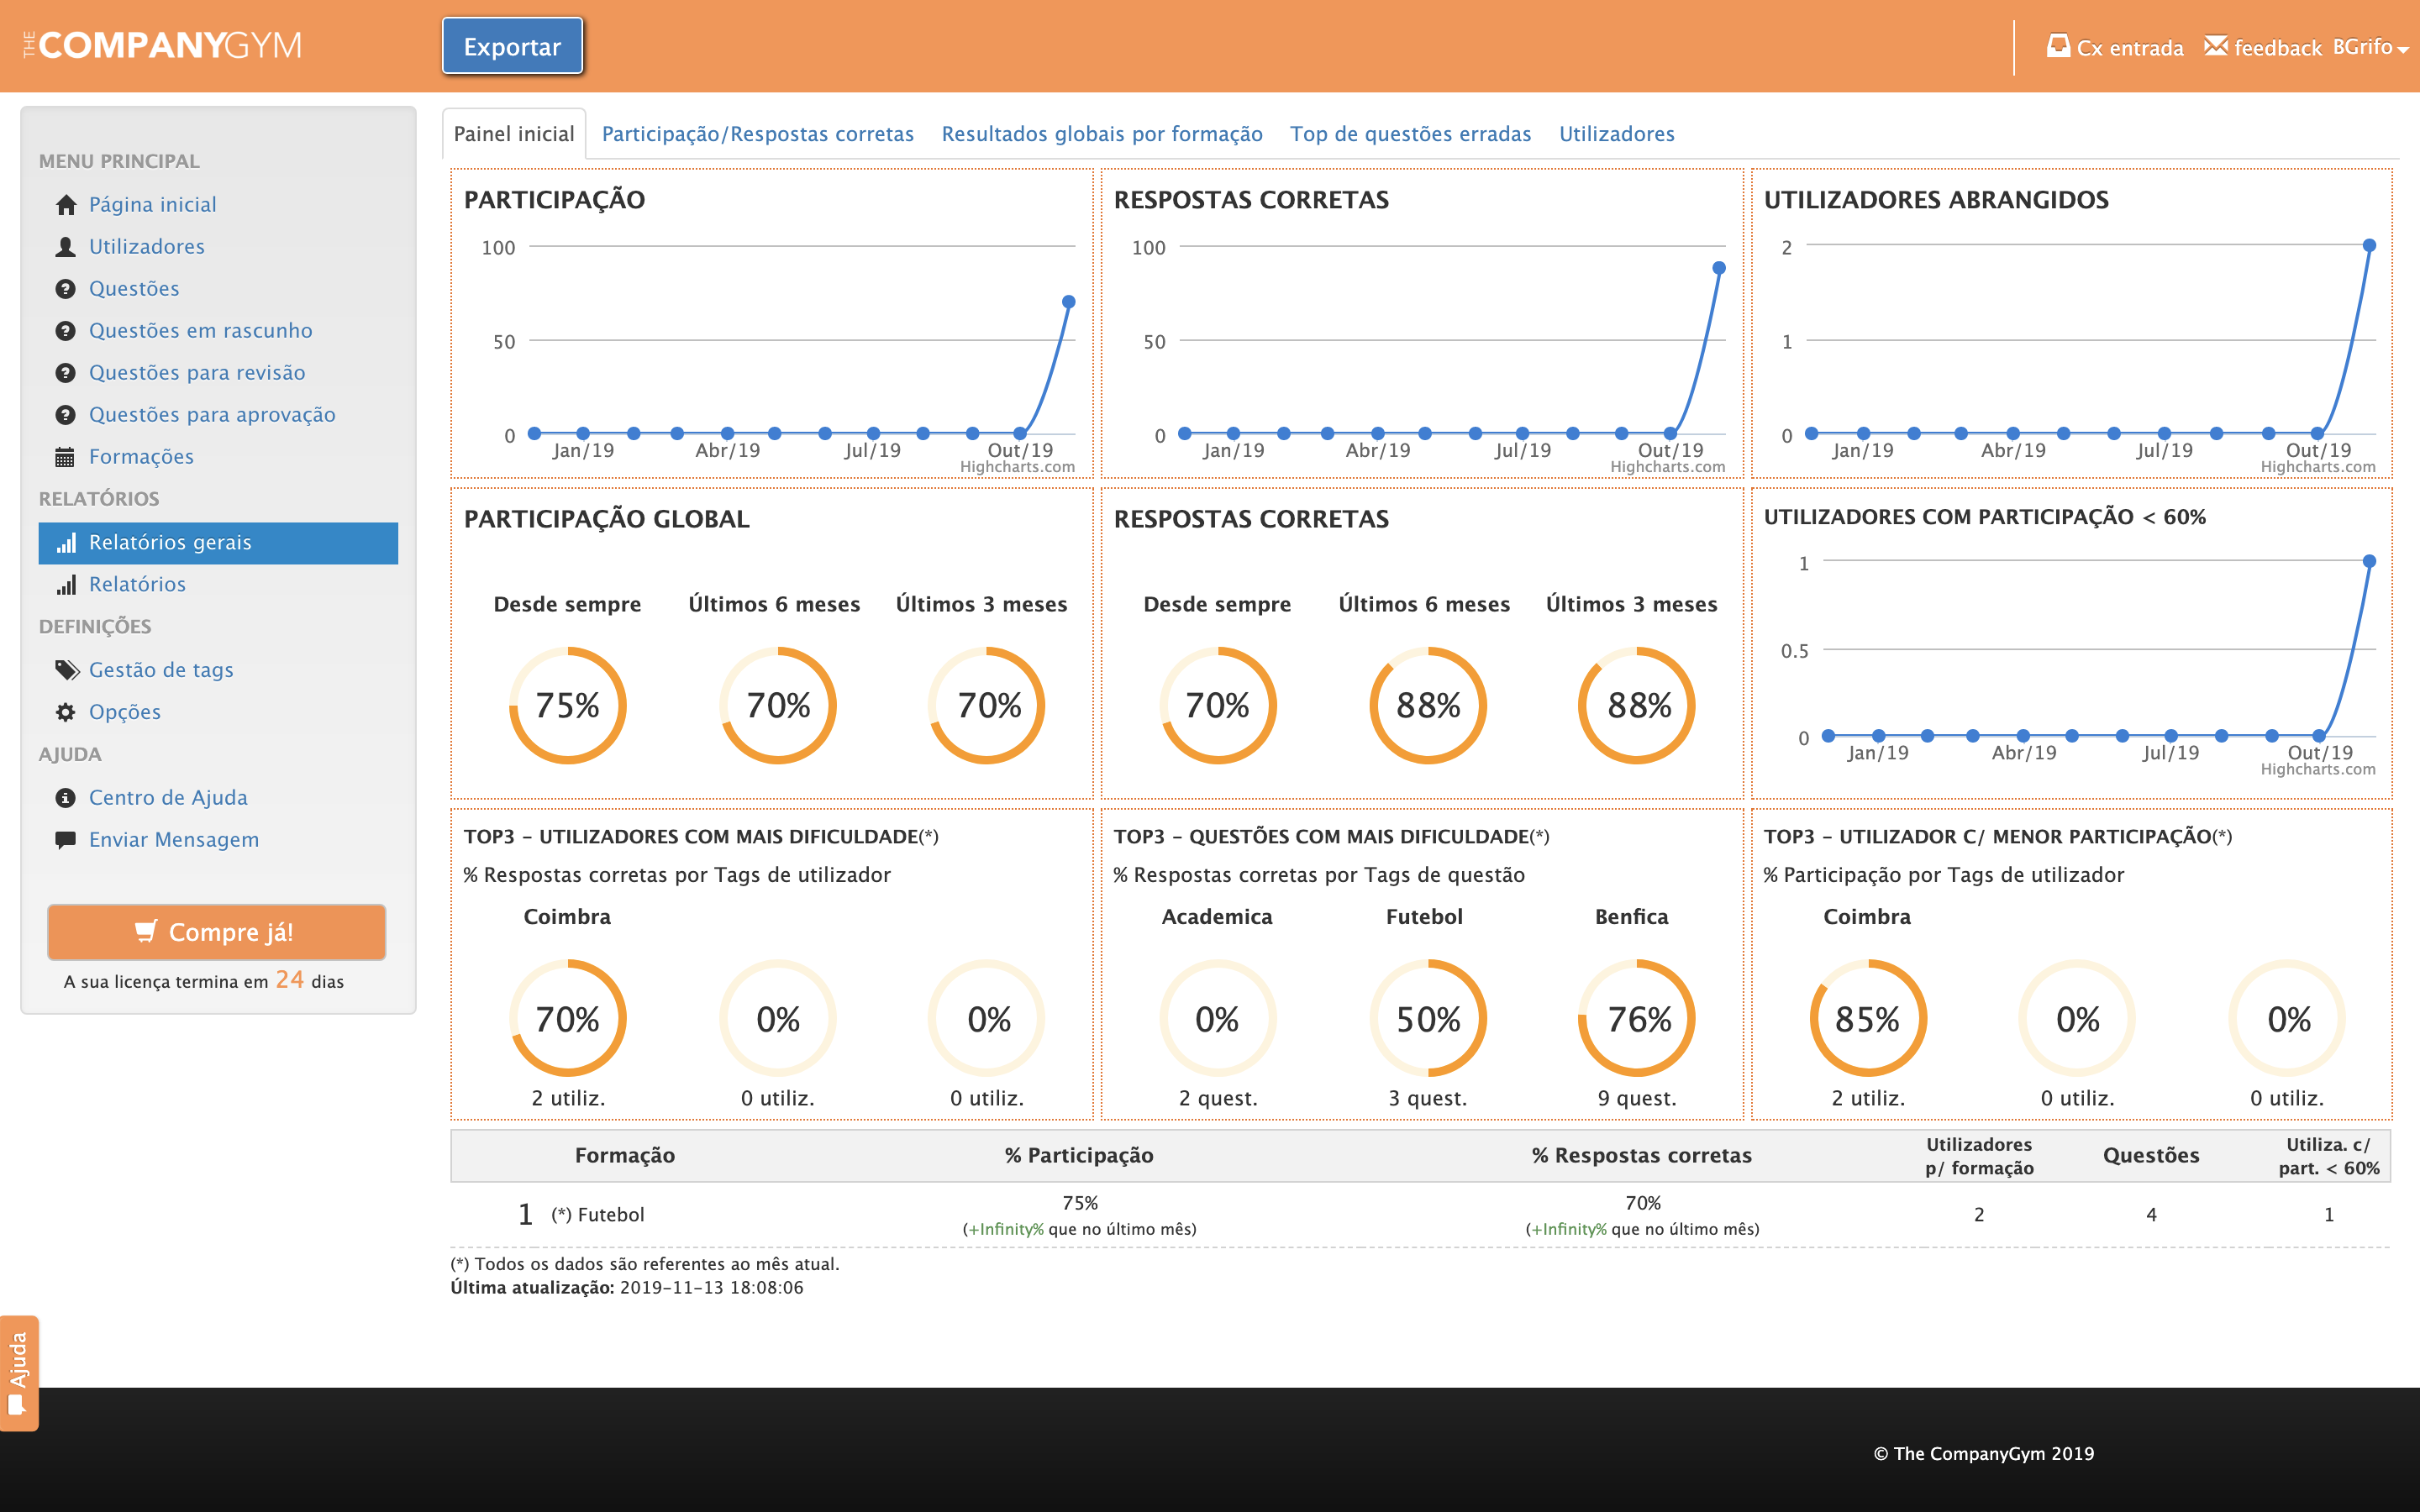
\includegraphics[width=1\textwidth]{img/tcg/tcg-data.png}
		\caption{The Company Gym - Relatório geral (Painel inicial)}
		\label{fig:tcg-data}
	\end{center}
\end{figure}

\newpage

\begin{figure}[ht!]
	\begin{center}
		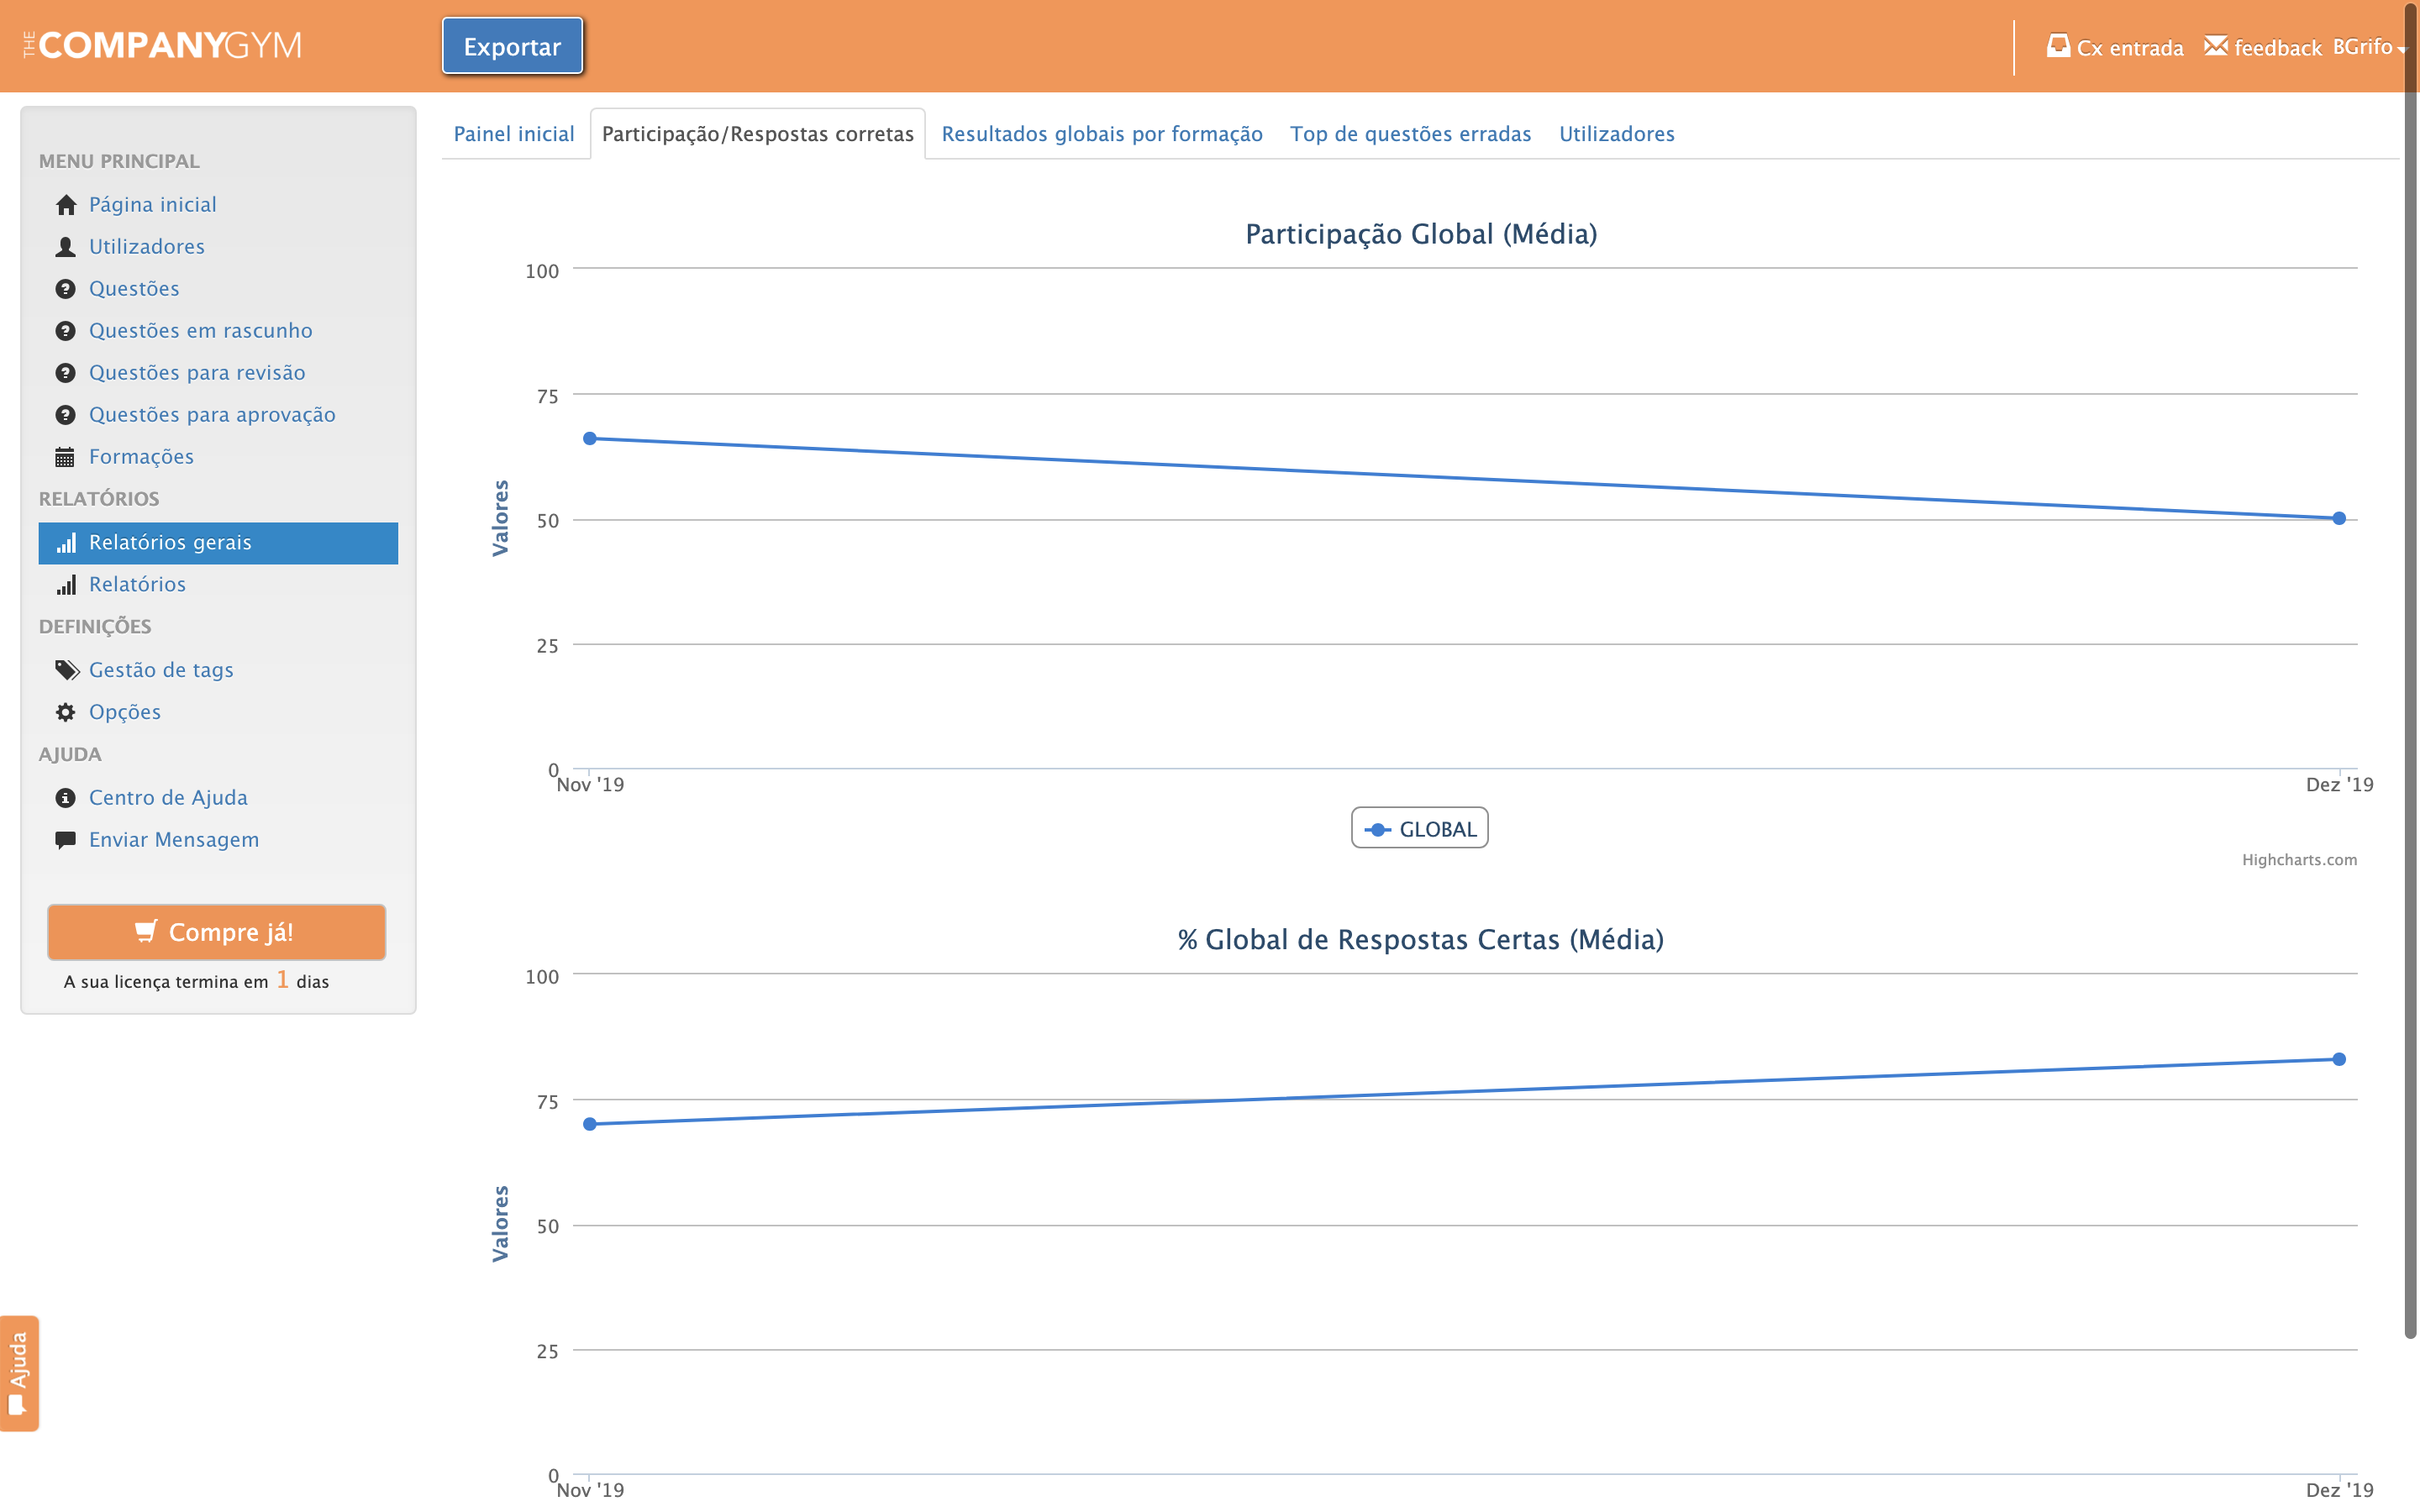
\includegraphics[width=1\textwidth]{img/tcg/tcg-data1.png}
		\caption{The Company Gym - Relatório geral (Participação/Respostas correctas)}
		\label{fig:tcg-data1}
	\end{center}
\end{figure}

Nas Figuras \ref{fig:tcg-data1} e \ref{fig:tcg-data2} temos representados a participação/respostas correctas de todas as formações e os resultados globais por formação, respectivamente.

\begin{figure}[ht!]
	\begin{center}
		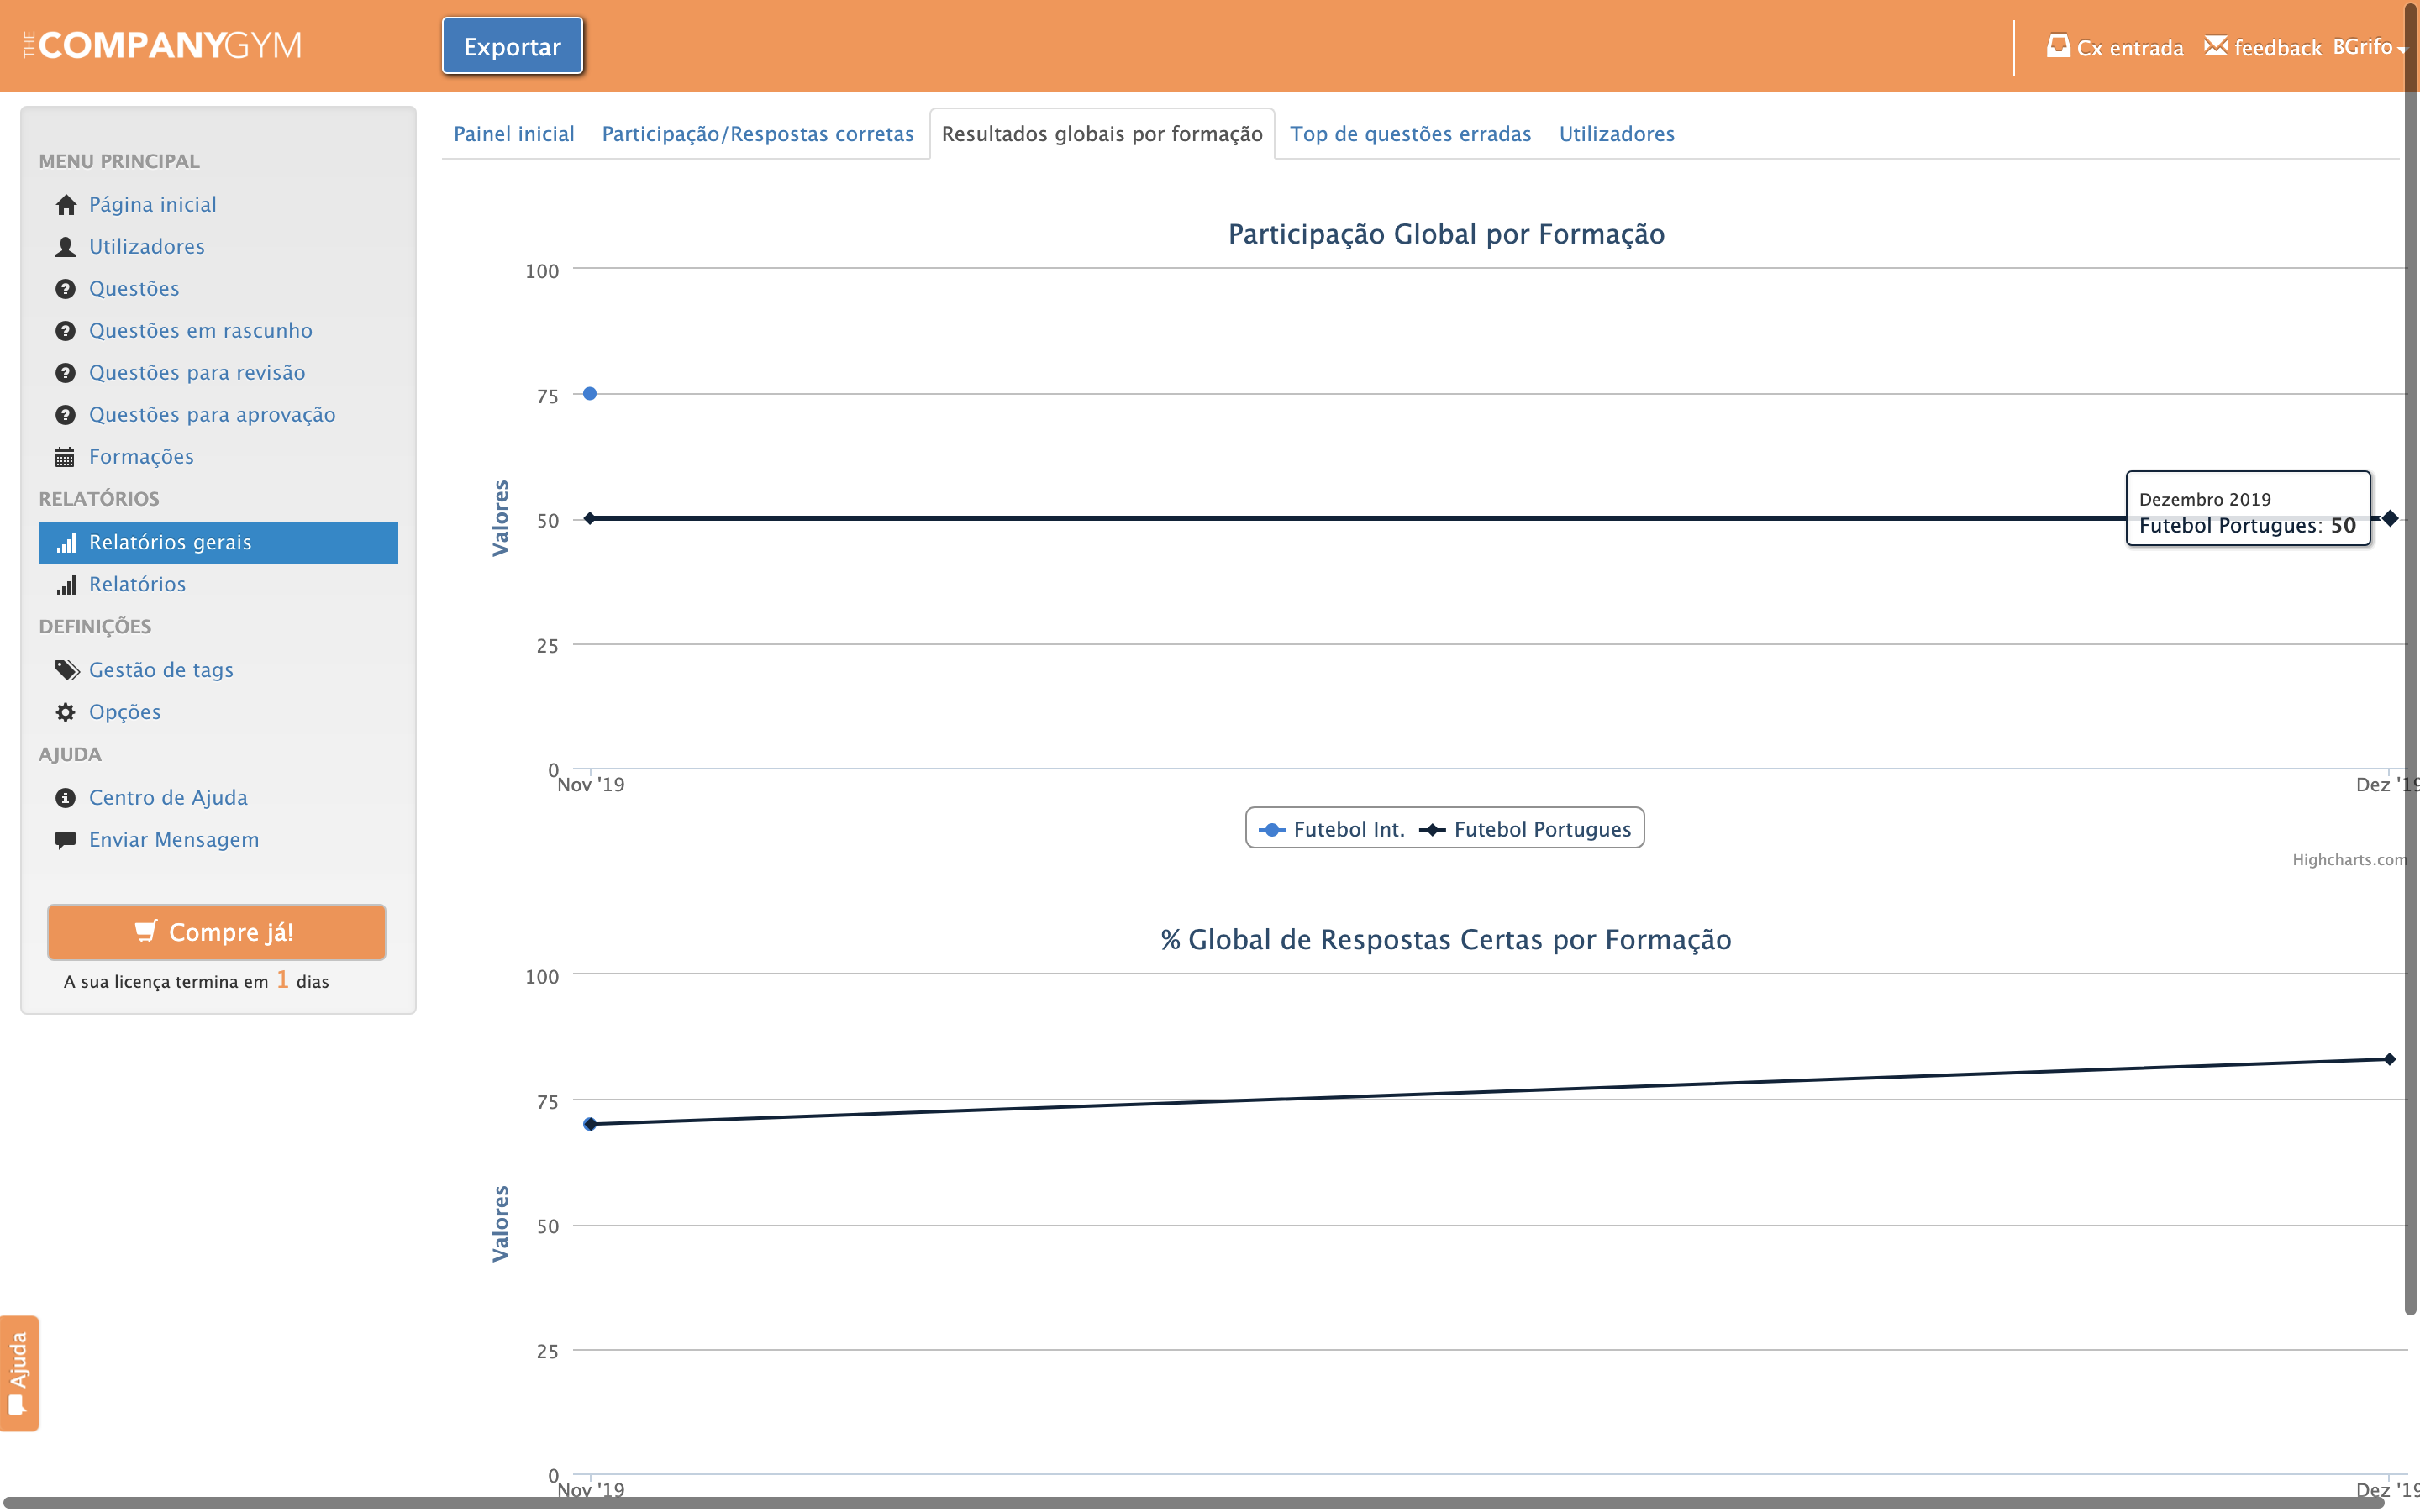
\includegraphics[width=1\textwidth]{img/tcg/tcg-data2.png}
		\caption{The Company Gym - Relatório geral (Resultados globais por formação)}
		\label{fig:tcg-data2}
	\end{center}
\end{figure}

\newpage


No relatório geral é também possível monitorizar quais as questões com maior número de respostas erradas e o desempenho de cada utilizador final, como podemos ver nas Figuras \ref{fig:tcg-data3} e \ref{fig:tcg-data4}, respectivamente, numa escala temporal definida pelo utilizador. 

\begin{figure}[ht!]
	\begin{center}
		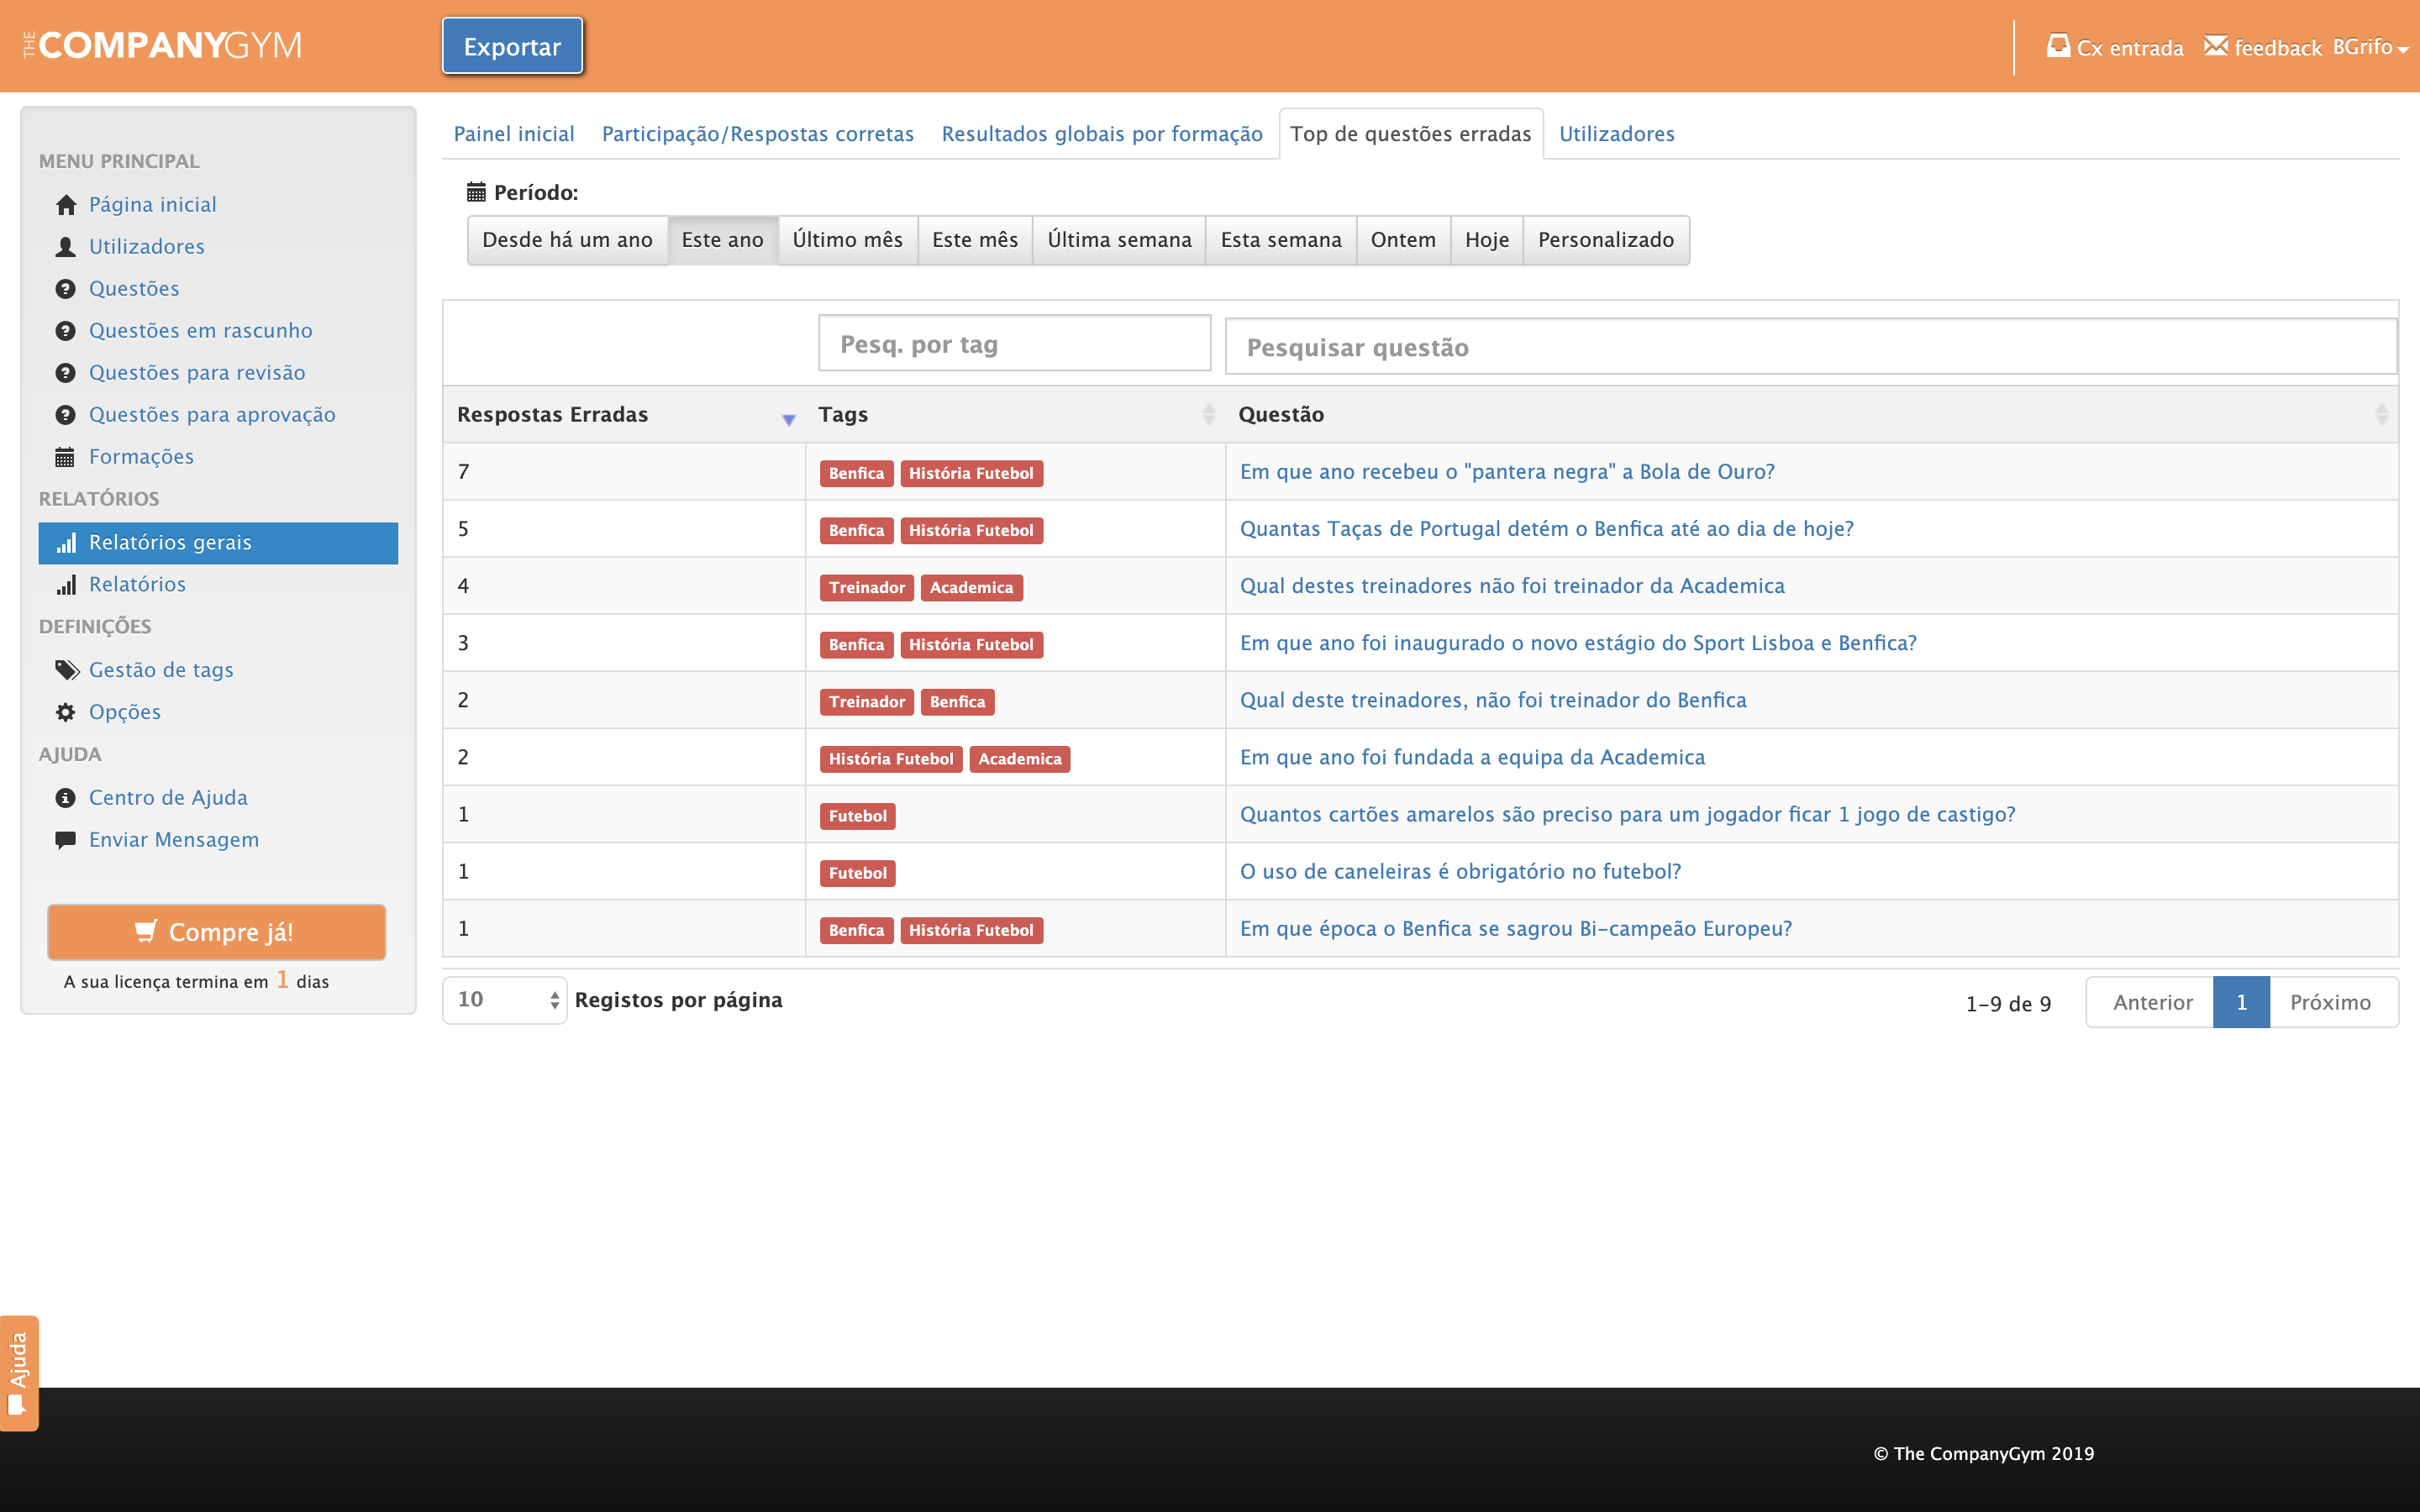
\includegraphics[width=1\textwidth]{img/tcg/tcg-data3.png}
		\caption{The Company Gym - Relatório geral (\textit{Top} de questões erradas)}
		\label{fig:tcg-data3}
	\end{center}
\end{figure}

\begin{figure}[ht!]
	\begin{center}
		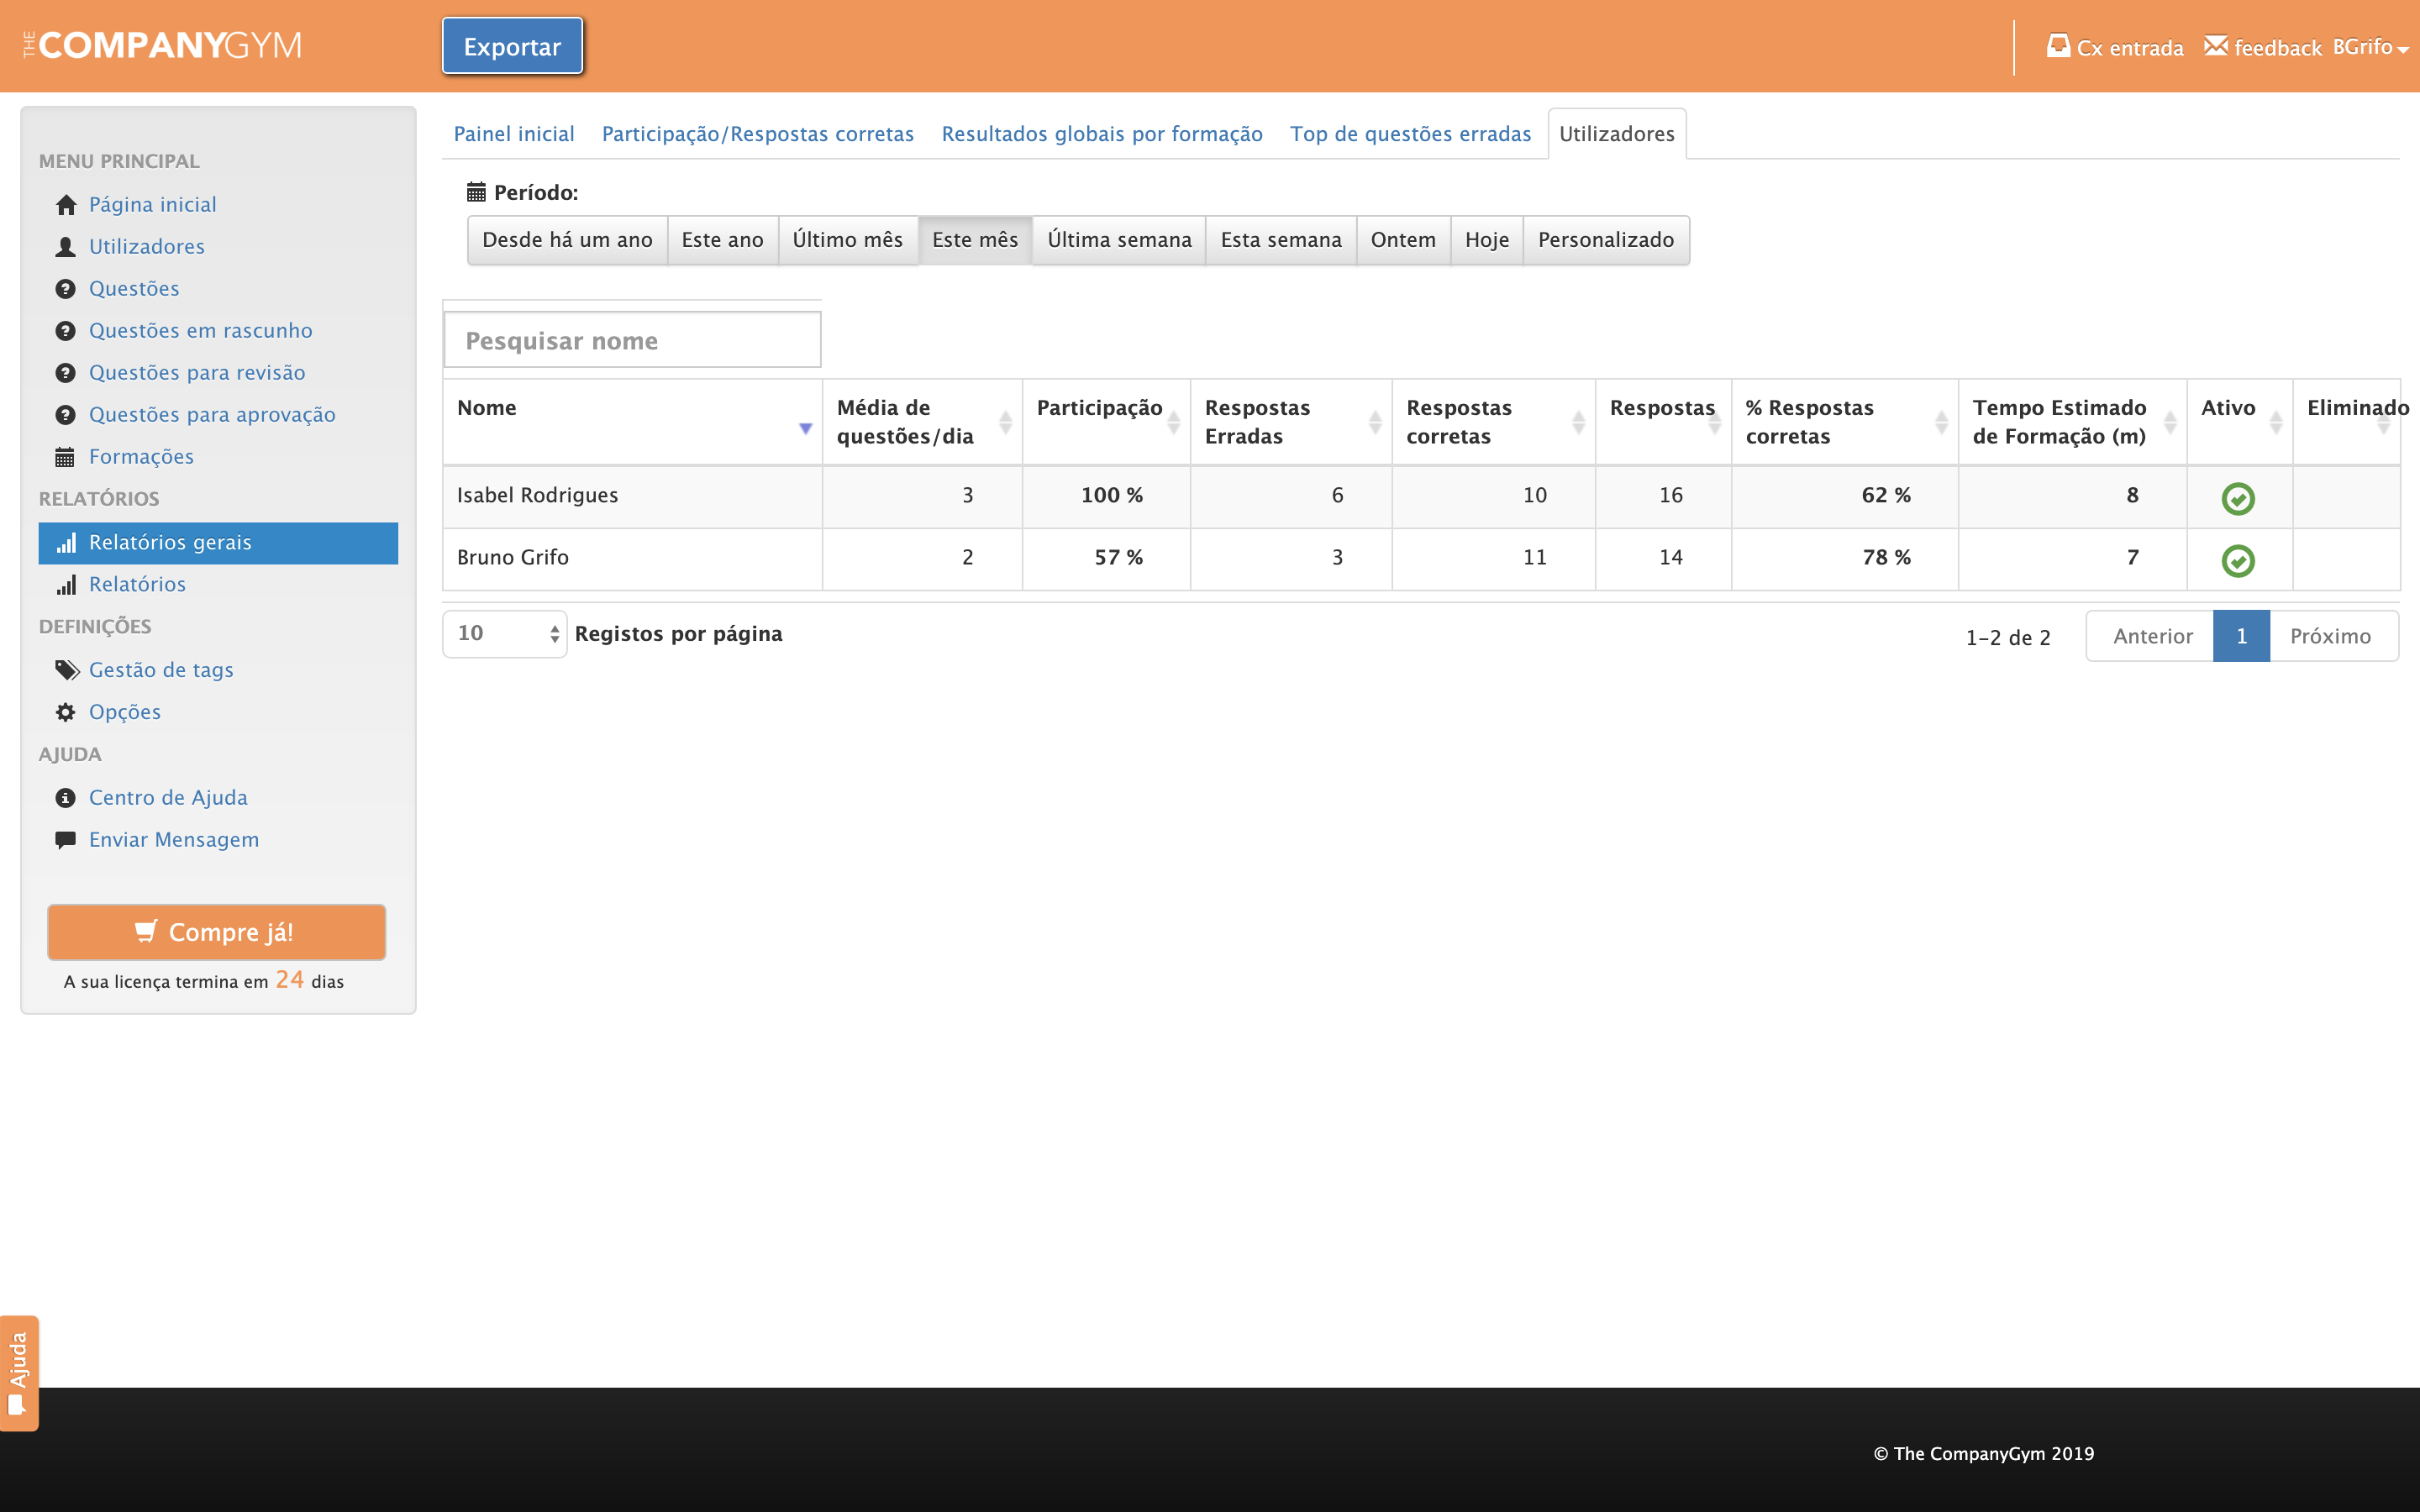
\includegraphics[width=1\textwidth]{img/tcg/tcg-data4.png}
		\caption{The Company Gym - Relatório geral (Utilizadores)}
		\label{fig:tcg-data4}
	\end{center}
\end{figure}

\newpage

Nos relatórios específicos para uma formação, o tratamento dos dados é muito semelhante como poderemos verificar mais em diante nas Figuras \ref{fig:tcg-data-f},  \ref{fig:tcg-data-f1}, \ref{fig:tcg-data-f2} e \ref{fig:tcg-data-f3}. Depois de selecionar a formação para ser possível gerar o relatório de dados, numa escala temporal definida pelo utilizador, são apresentados os gráficos relativos à percentagem de participação, respostas correctas por \textit{tag} de questão e utilizador. 
No \textit{top} de questões erradas é possível listar os utilizadores finais que erraram uma determinada pergunta. O inverso acontece na página seguinte, representado na Figura \ref{fig:tcg-data-f2}, sendo possível listar as questões onde os utilizadores com mais respostas erradas, erraram. 
Por fim temos a listagem dos utilizadores finais que estão associados à formação em questão, seguidos das estatísticas relacionadas com o seu desempenho.

\begin{figure}[ht!]
	\begin{center}
		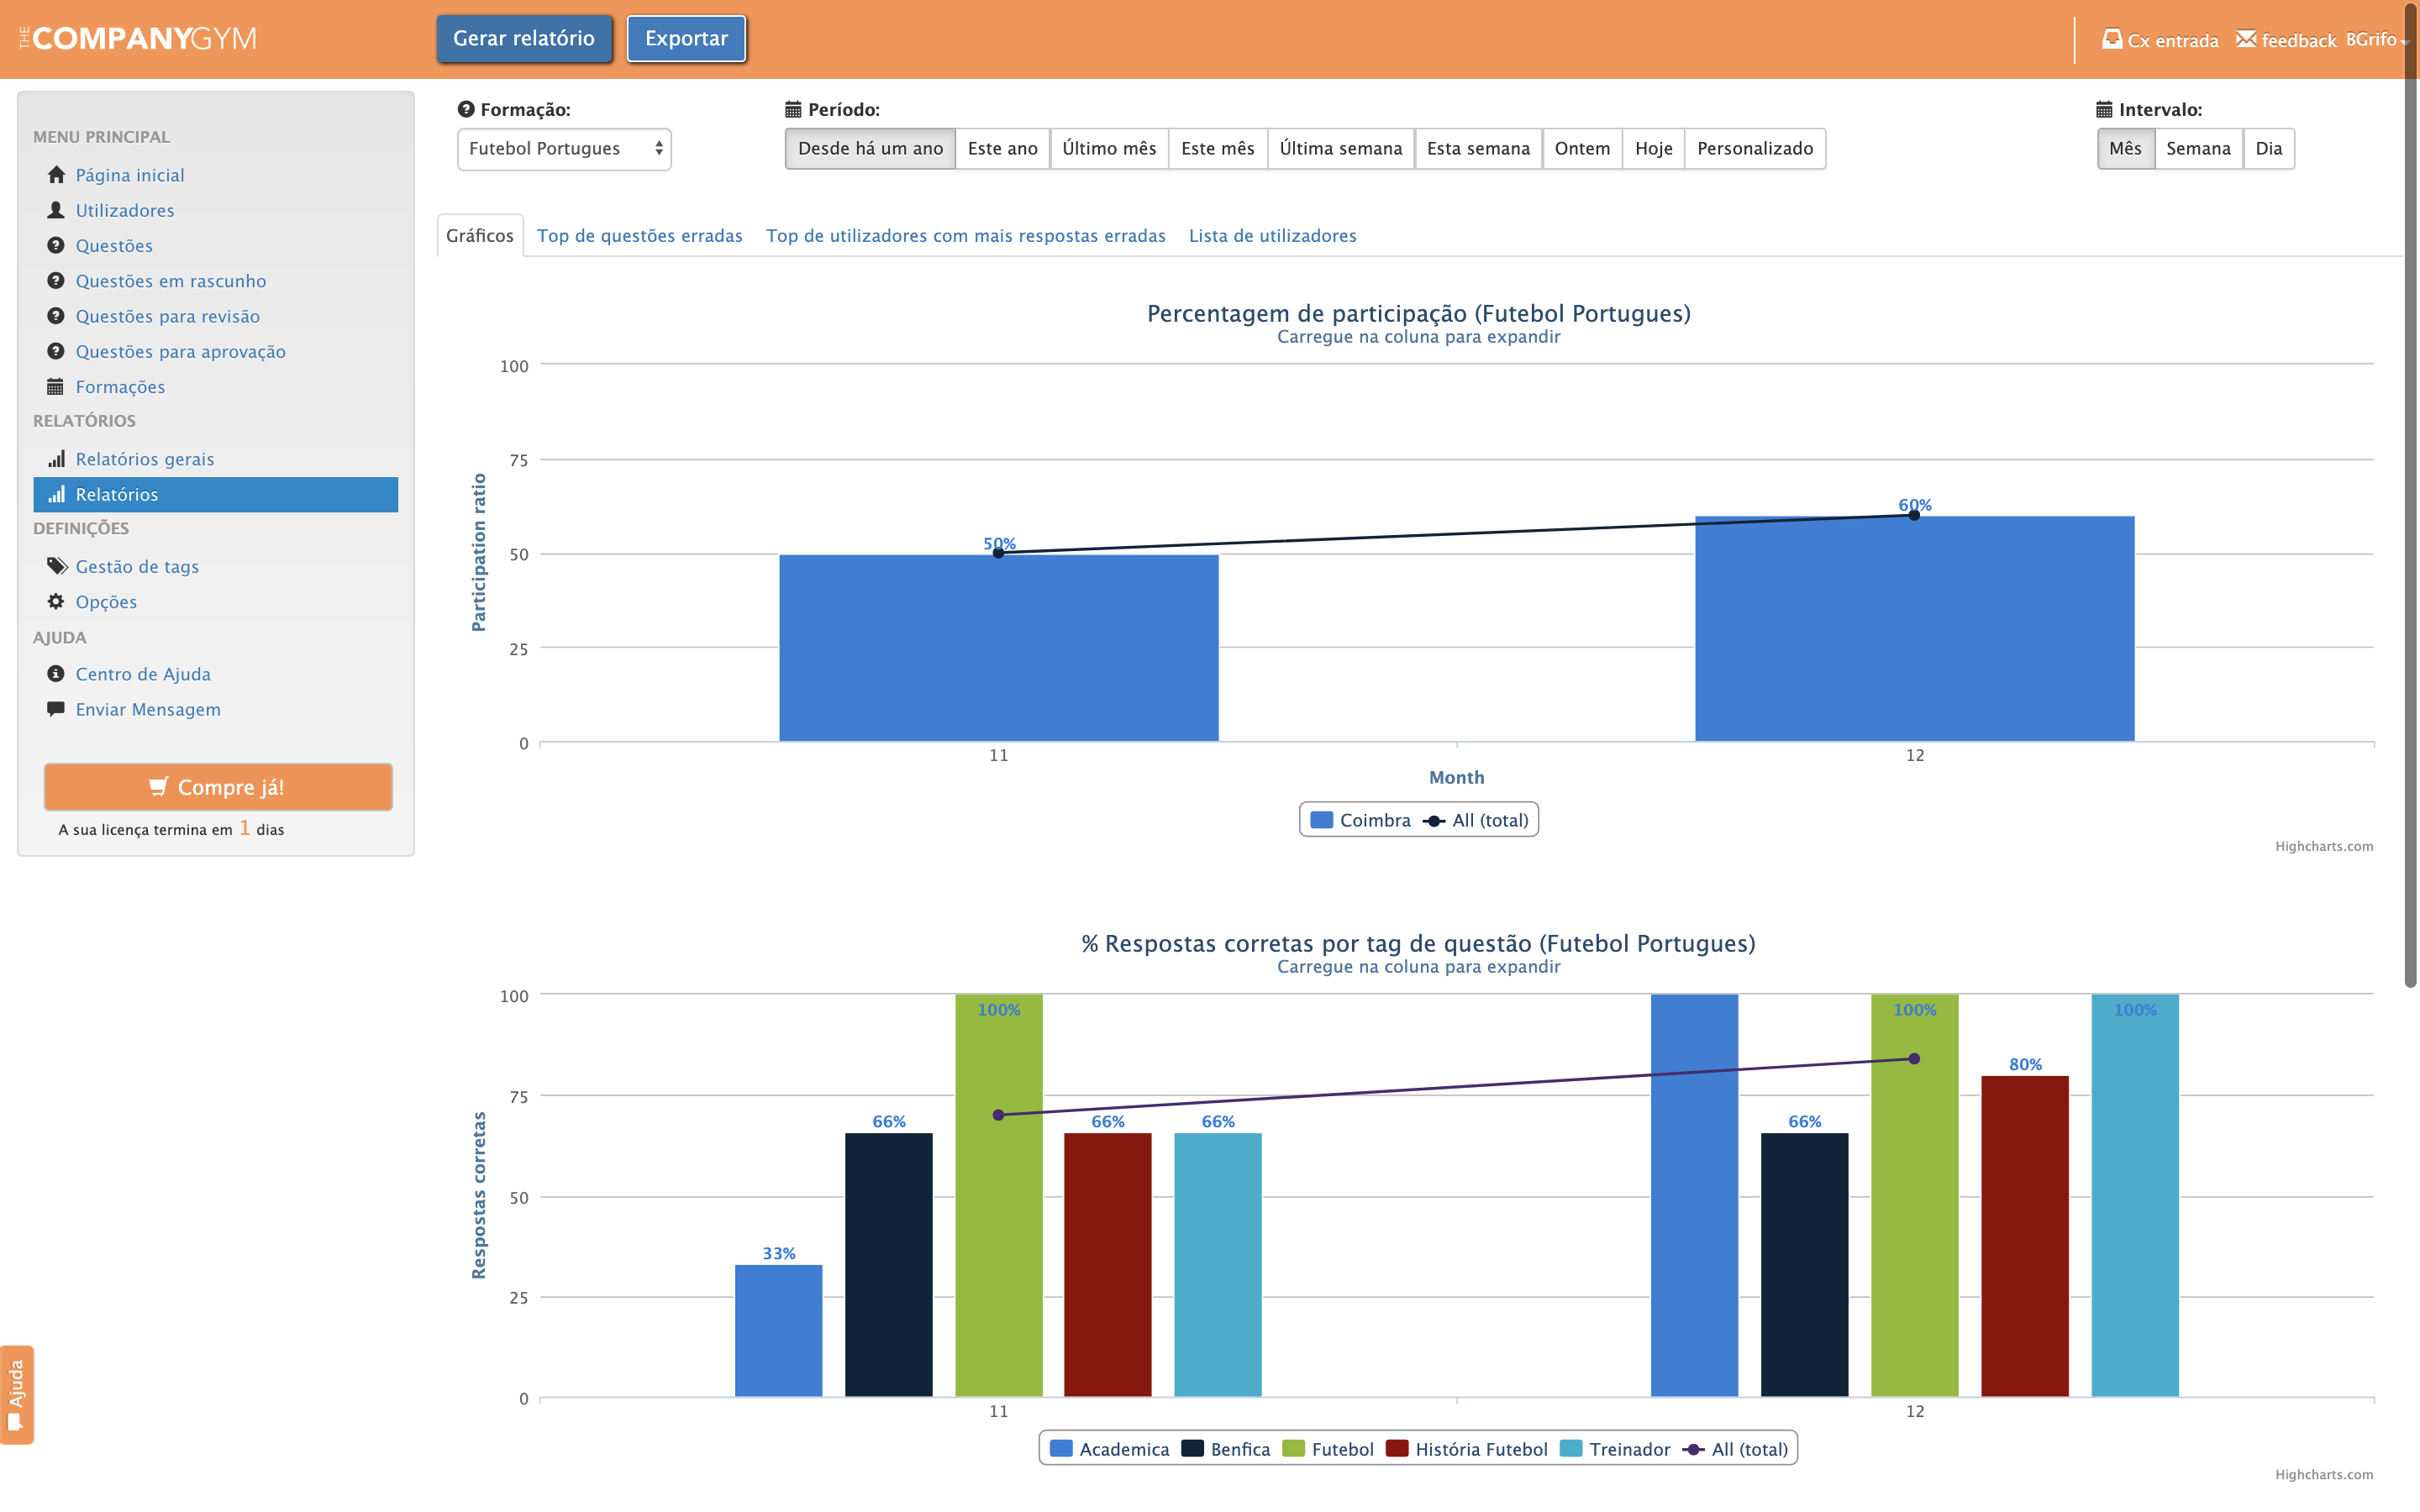
\includegraphics[width=1\textwidth]{img/tcg/tcg-data-f.png}
		\caption{The Company Gym - Relatório específico de uma formação (Gráficos)}
		\label{fig:tcg-data-f}
	\end{center}
\end{figure}
\pagebreak

\begin{figure}[ht!]
	\begin{center}
		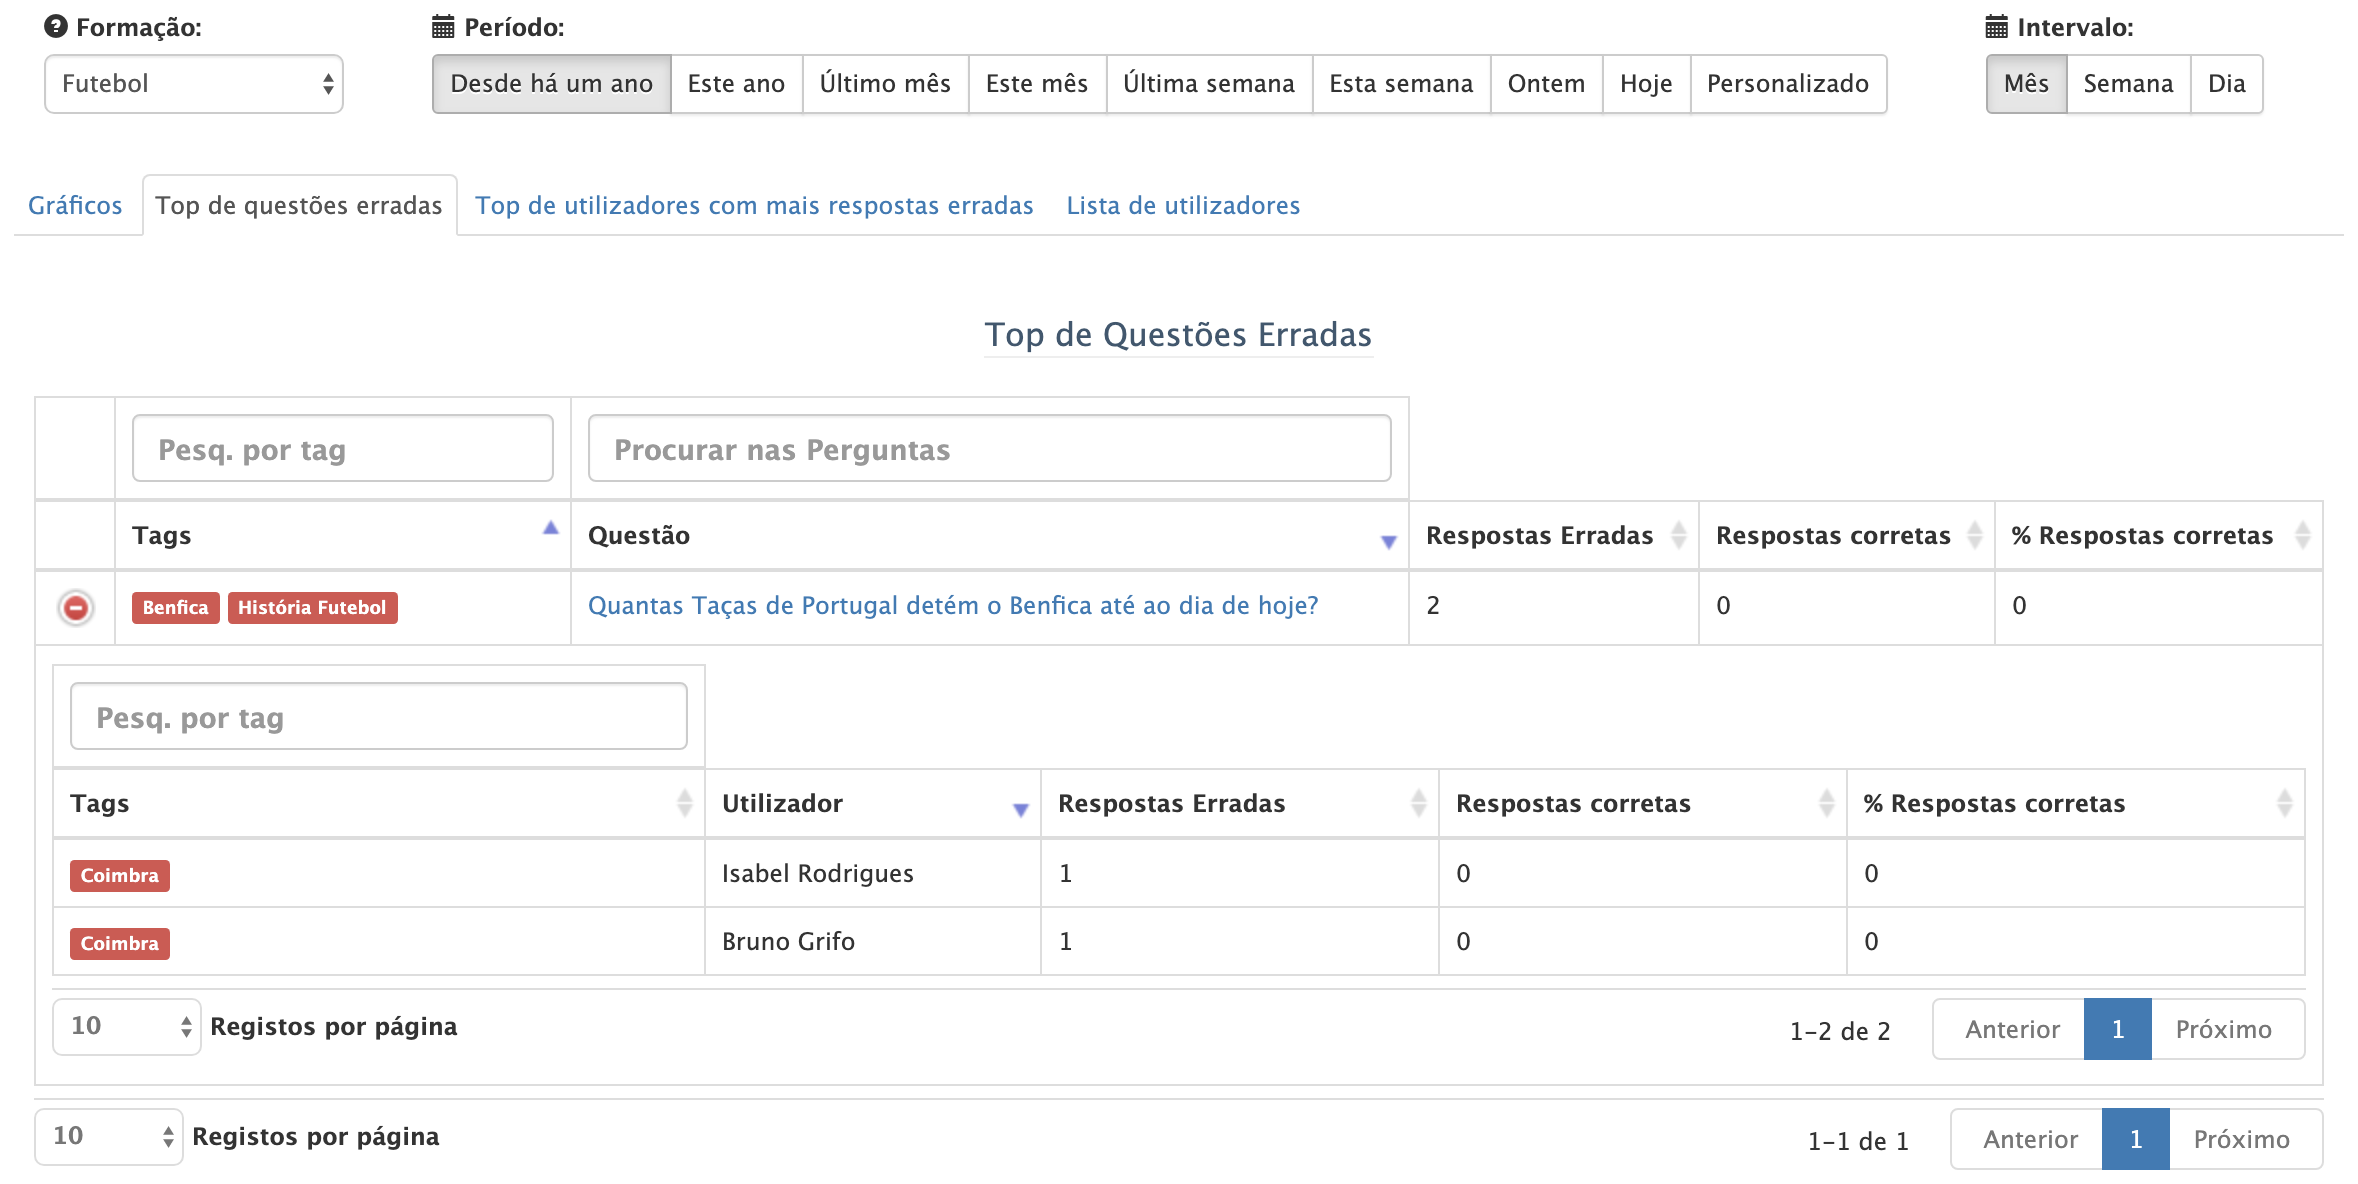
\includegraphics[width=1\textwidth]{img/tcg/tcg-data-f1.png}
		\caption{The Company Gym - Relatório específico de uma formação (\textit{Top} de questões erradas)}
		\label{fig:tcg-data-f1}
	\end{center}
\end{figure}
\mbox{}
\begin{figure}[ht!]
	\begin{center}
		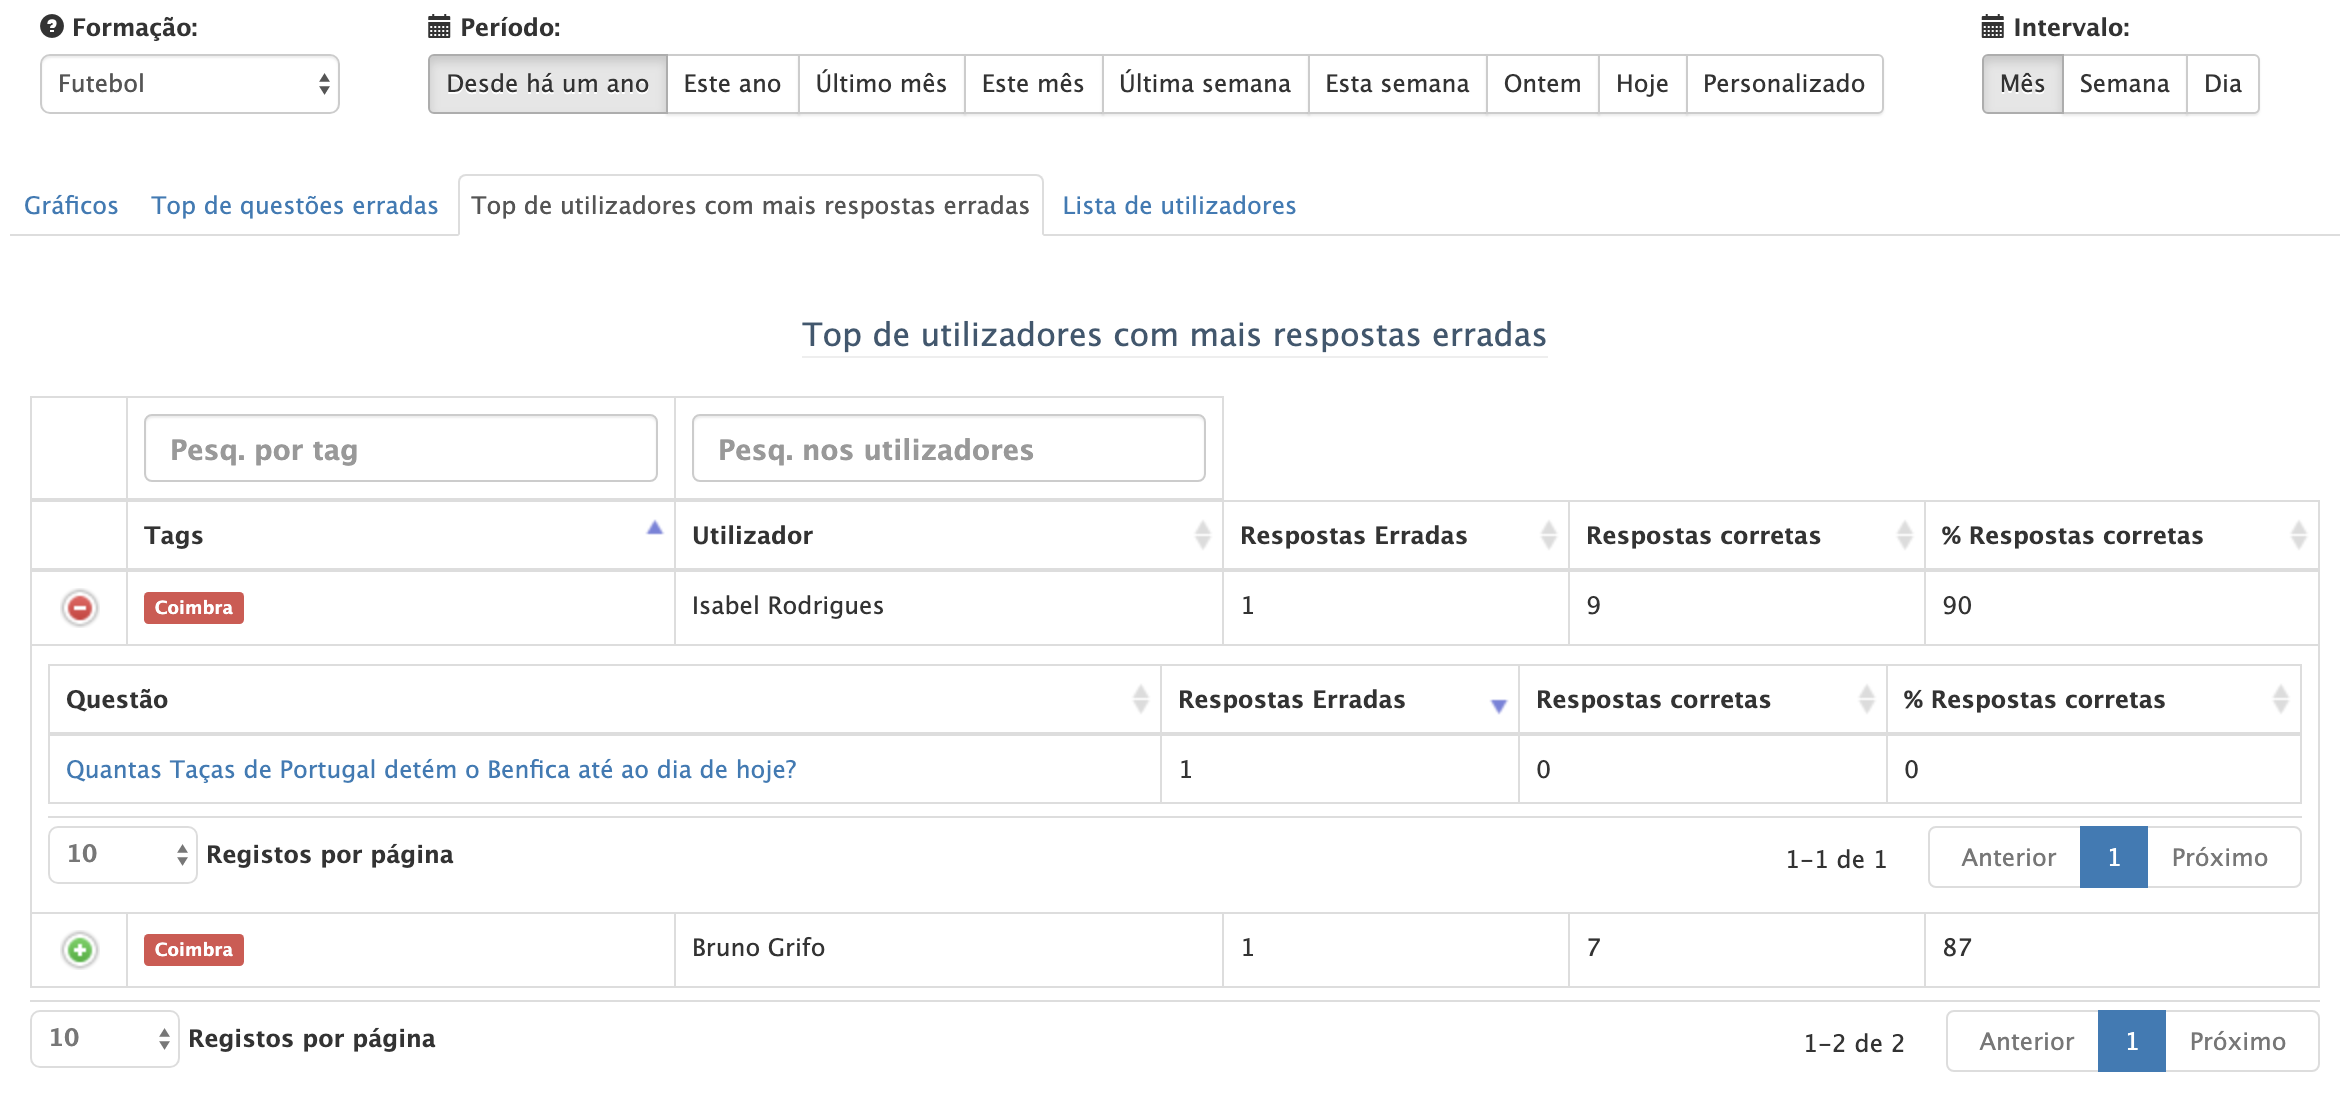
\includegraphics[width=1\textwidth]{img/tcg/tcg-data-f2.png}
		\caption{The Company Gym - Relatório específico de uma formação (\textit{Top} de utilizadores com mais respostas erradas)}
		\label{fig:tcg-data-f2}
	\end{center}
\end{figure}

\newpage
\begin{figure}[ht!]
	\begin{center}
		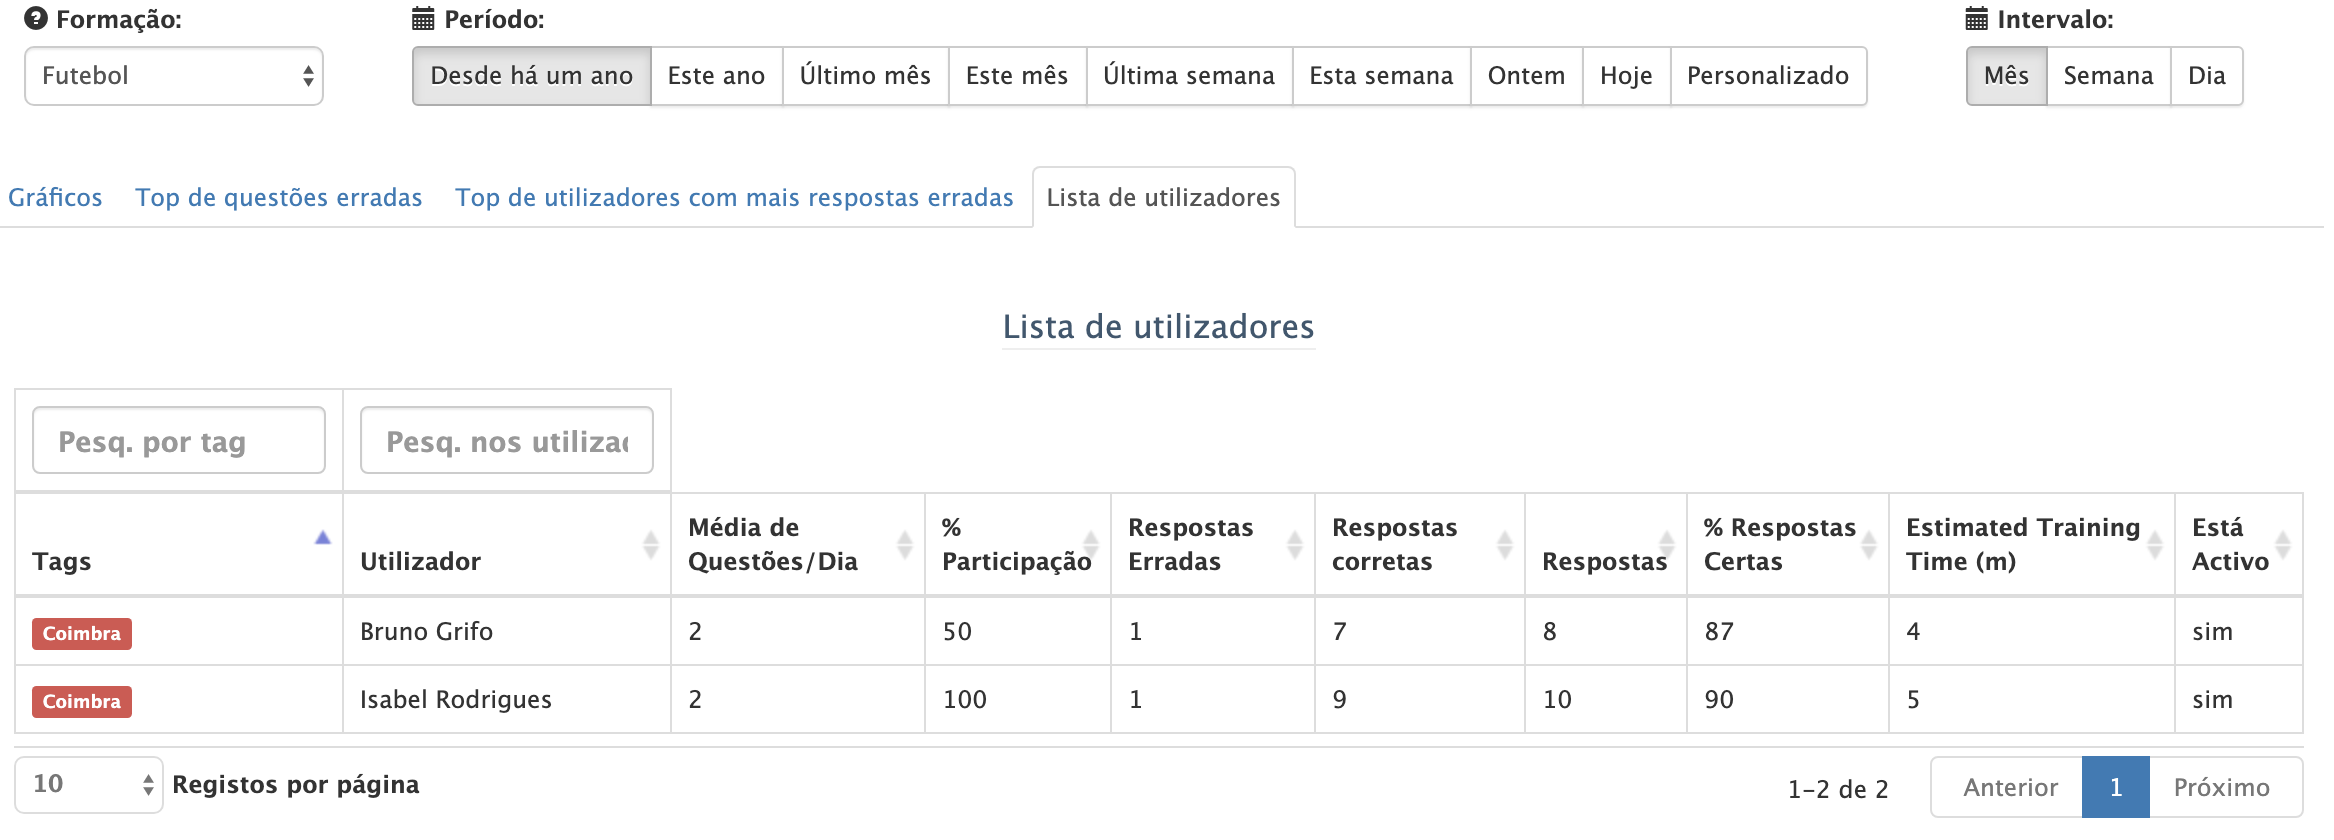
\includegraphics[width=1\textwidth]{img/tcg/tcg-data-f3.png}
		\caption{The Company Gym - Relatório específico de uma formação (Lista de utilizadores)}
		\label{fig:tcg-data-f3}
	\end{center}
\end{figure}



\section{involve.me}
\label{involveme}


"\textit{involve.me is a next-generation user engagement \& customer experience platform with a focus on digital marketers \& e-commerce.}"\cite{involve}.
Esta plataforma foca-se também em recolher e analisar informações sobre os utilizadores finais.

O involve.me oferece um plano gratuito com 100 submissões por mês e acesso limitado às funcionalidades da plataforma. Para aceder às funcionalidades da plataforma é necessário criar um conta.

Para testar as funcionalidades desta ferramenta, foi criado um questionário para calcular o local ideal para passar férias consoante as preferências do utilizador final. 


Uma das funcionalidades interessantes do involve.me é a criação de questionários que por exemplo, consoante as respostas do utilizador final, o resultado vai ser diferente, tal como podemos ver nas Figuras \ref{fig:ivme-x1} e \ref{fig:ivme-x2}.
\newpage


\begin{figure}[ht!]
	\begin{center}
		\includegraphics[width=1\textwidth]{img/ivme/x1}
		\caption{involve.me - Exemplo de um Questionário}
		\label{fig:ivme-x1}
	\end{center}
\end{figure}

\begin{figure}[ht!]
	\begin{center}
		\includegraphics[width=1\textwidth]{img/ivme/x2}
		\caption{involve.me - Resultado do Questionário da Figura \ref{fig:ivme-x2}}
		\label{fig:ivme-x2}
	\end{center}
\end{figure}

\pagebreak

A partir da página principal, como podemos ver na Figura \ref{fig:ivme-dash} temos listados todos os projetos do utilizador. A partir da página principal podemos também criar um novo projeto, aceder à lista de \textit{templates} (Figura \ref{fig:ivme-templares}) recomendados para os projetos, análise dos resultados dos projetos, integrações (i. e. com sistemas externos) e informações e definições da conta do utilizador. 

\begin{figure}[ht!]
	\begin{center}
		\includegraphics[width=1\textwidth]{img/ivme/dashboard}
		\caption{involve.me - Página Principal}
		\label{fig:ivme-dash}
	\end{center}
\end{figure}

\begin{figure}[ht!]
	\begin{center}
		\includegraphics[width=1\textwidth]{img/ivme/templates}
		\caption{involve.me -Templates}
		\label{fig:ivme-templares}
	\end{center}
\end{figure}


Representado na Figura \ref{fig:ivme-elements} temos o início do processo da criação de um questionário para mostrar a um utilizador final um destino para passar férias. Outras experiências podem ser criadas (e. g. formulário, \textit{survey} etc...), contudo serão apenas mostradas as funcionalidades chaves que competem com o 10.quest. Como podemos ver é possível adicionar vários tipos de elementos e personalizá-los ao gosto do utilizador. 


\begin{figure}[ht!]
	\begin{center}
		\includegraphics[width=1\textwidth]{img/ivme/elements}
		\caption{involve.me - Elementos}
		\label{fig:ivme-elements}
	\end{center}
\end{figure}

Como foi referido anteriormente o involve.me permite a criação de questionários que consoante as respostas do utilizador final, devolve uma determinada resposta. Para isso é necessário associar as respectivas respostas às perguntas. Em primeiro lugar é necessário selecionar o elemento para que seja possível editar o mesmo, tal como podemos ver na Figura \ref{fig:ivme-associar}.

Os resultados têm de ser criados previamente antes de serem associados às respostas do questionário. Como podemos ver na Figura \ref{fig:ivme-result} um resultado pode ser composto por um conjunto de elementos. 

É ainda de notar que o involve.me permite a adição de pontuação às respostas, permitindo assim criar um sistema de pontuação que possibilita atribuir maior relevância a uma ou mais respostas.

 Antes de publicar o questionário é possível fazer uma pré-visualização para verificar se o questionário cumpre as necessidades do utilizador. O involve.me permite a pré-visualização dos \textit{items}/experiências em dispositivos móveis e computador como podemos ver na Figura \ref{fig:ivme-preview}.
 
\newpage
\begin{figure}[ht!]
	\begin{center}
		\includegraphics[width=1\textwidth]{img/ivme/associar}
		\caption{involve.me - Associar resultados às respostas}
		\label{fig:ivme-associar}
	\end{center}
\end{figure}

\begin{figure}[ht!]
	\begin{center}
		\includegraphics[width=1\textwidth]{img/ivme/result}
		\caption{involve.me - Resultado possível}
		\label{fig:ivme-result}
	\end{center}
\end{figure}
 
 \begin{figure}[ht!]
 	\begin{center}
 		\includegraphics[width=1\textwidth]{img/ivme/preview}
 		\caption{involve.me - Pré-visualização do questionário}
 		\label{fig:ivme-preview}
 	\end{center}
 \end{figure}
\newpage

Depois de terminar o questionário, tal como podemos ver nas Figuras \ref{fig:ivme-project} e \ref{fig:ivme-social}, é necessário definir algumas informações sobre o mesmo (e. g. nome, URL, validade etc..)e é ainda possível criar um \textit{template} com o título e descrição para ser partilhado nas redes sociais. O questionário pode também ser partilhado através de um URL ou embebido noutro \textit{website}.


\begin{figure}[ht!]
	\begin{center}
		\includegraphics[width=1\textwidth]{img/ivme/project}
		\caption{involve.me - Definições do projeto}
		\label{fig:ivme-project}
	\end{center}
\end{figure}

\begin{figure}[ht!]
	\begin{center}
		\includegraphics[width=1\textwidth]{img/ivme/social}
		\caption{involve.me - Template para as redes sociais}
		\label{fig:ivme-social}
	\end{center}
\end{figure}


Na secção de análise de dados, o involve.me apresenta as estatísticas gerais de todos os projectos do utilizador, dando uma percepção acerca da participação geral nos mesmos. É também possível selecionar um dos projetos do utilizador e assim gerar e visualizar os resultados, como podemos ver nas Figuras \ref{fig:ivme-overall1} e \ref{fig:ivme-results1}.

No sumário de respostas é possível ver quais as respostas mais frequentes, contudo o mesmo resultado não se consegue verificar para o resultado final (i. e. não é possível visualizar quais os resultados mais frequentes). As respostas detalhadas, tal como os dados pessoais, apresentam todas as respostas de um respetivo utilizador final. 

\newpage

\begin{figure}[ht!]
	\begin{center}
		\includegraphics[width=1\textwidth]{img/ivme/overall1}
		\caption{involve.me - Estatísticas gerais do quesitonário}
		\label{fig:ivme-overall1}
	\end{center}
\end{figure}

\begin{figure}[ht!]
	\begin{center}
		\includegraphics[width=1\textwidth]{img/ivme/results1}
		\caption{involve.me - Sumário de respostas do questionário}
		\label{fig:ivme-results1}
	\end{center}
\end{figure}


\subsection{Survey Anyplace}
\label{surveyanyplaceM}



O Survey Anyplace é uma plataforma online com foco na criação de \textit{surveys} e questionários interativos. O Survey Anyplace afirma proporcionar uma boa experiência para o utilizador através de elementos interativos e funcionalidades de personalização. Esta plataforma permite também a análise dos dados recolhidos através dos questionários publicados. Apesar de não ser fornecido nenhum plano gratuito, o Survey Anyplace disponibiliza um trial de 6 dias que fornece acesso a grande parte das funcionalidades.

Como podemos ver na Figura \ref{fig:sap-dash}, na página principal temos acesso aos questionários do utilizador. O utilizador a partir desta página consegue criar um novo questionário, editar e eliminar um questionário já existente. A partir daqui o utilizar consegue também aceder à sua conta onde pode atualizar/alterar as suas informações básicas(e. g. nome, email, idioma etc..). 


\begin{figure}[ht!]
	\begin{center}
		\includegraphics[width=1\textwidth]{img/sap/dash}
		\caption{Survey Anyplace - Página inicial}
		\label{fig:sap-dash}
	\end{center}
\end{figure}

Na Figura \ref{fig:sap-create} está representado o processo de criação de um questionário na plataforma. No exemplo estão apenas representados dois tipos de perguntas (i. e. escolha múltipla de texto e de imagens), contudo outros géneros de perguntas podem ser adicionados como podemos ver na Figura \ref{fig:sap-type}. A plataforma permite anexar ficheiros às perguntas e respostas através de um link, redes sociais ou do dispositivo do utilizador, sendo que para as perguntas estes ficheiros podem ser imagens ou vídeos e para as respostas apenas são aceites imagens.

Ainda na Figura \ref{fig:sap-create} podemos verificar que é possível atribuir uma pontuação a uma resposta, e de seguida associar a mesma a um resultado. Desta forma é criado um sistema de pontuação que baseado nas respostas do utilizador, irá apresentar o resultado com maior pontuação. Outras definições tais como permitir mais do que uma resposta, tornar uma pergunta mandatória, etc.. são acessíveis nesta página.

\newpage

\begin{figure}[ht!]
	\begin{center}
		\includegraphics[width=1\textwidth]{img/sap/create}
		\caption{Survey Anyplace - Criar questionário}
		\label{fig:sap-create}
	\end{center}
\end{figure}

\begin{figure}[ht!]
	\begin{center}
		\includegraphics[width=1\textwidth]{img/sap/type}
		\caption{Survey Anyplace - Tipo de pergunta}
		\label{fig:sap-type}
	\end{center}
\end{figure}
\pagebreak

Na secção \textit{Design} encontra-se todas as funcionalidades relacionadas com a personalização do template, tal como podemos ver na Figura \ref{fig:sap-design}

\begin{figure}[ht!]
	\begin{center}
		\includegraphics[width=1\textwidth]{img/sap/design}
		\caption{Survey Anyplace - Personalização do questionário}
		\label{fig:sap-design}
	\end{center}
\end{figure}

O Survey Anyplace disponibiliza ainda uma série de funcionalidades extra para os questionários ( Figura \ref{fig:sap-extra} ). Algumas destas funcionalidades são importantes e visto que partilham um comportamento semelhante com a plataforma a desenvolver. Neste sentido algumas destas funcionalidades foram analisadas ao pormenor:
\begin{itemize}
	\item[--] \textbf{Condições lógicas} - Representado na Figura \ref{fig:sap-condicao} temos a implementação de uma condição lógica em que se duas condições se confirmarem então o utilizador será redirecionado para uma a pergunta definida. Esta e outras acções estão disponíveis dando ao utilizador possibilidade de, através de condições, criar um fluxo ou comportamento desejado.
	\item[--] \textbf{Resultados} - Como foi referido anteriormente é possível adicionar resultados a respostas é nesta secção que os resultados podem ser criados. Representado na Figura \ref{fig:sap-outcome} temos a criação de um resultado. É ainda de notar que em adição ao sistema de pontuações pode-se adicionar condições lógicas aos resultados para restringir os mesmos às necessidades do utilizador.
	\item[--] \textbf{Email} - Outra funcionalidade do Survey Anyplace é a possibilidade de enviar um email personalizado para um utilizador final. À semelhança da funcionalidade anterior pode-se adicionar condições lógicas aos templates para restringir os mesmos às necessidades do utilizador.
\end{itemize}

\newpage

\begin{figure}[ht!]
	\begin{center}
		\includegraphics[width=1\textwidth]{img/sap/extra}
		\caption{Survey Anyplace - Opções extra }
		\label{fig:sap-extra}
	\end{center}
\end{figure}
\mbox{}
\begin{figure}[ht!]
	\begin{center}
		\includegraphics[width=1\textwidth]{img/sap/condicao}
		\caption{Survey Anyplace - Condição lógica}
		\label{fig:sap-condicao}
	\end{center}
\end{figure}

\begin{figure}[ht!]
	\begin{center}
		\includegraphics[width=1\textwidth]{img/sap/outcome}
		\caption{Survey Anyplace - Resultados possíveis}
		\label{fig:sap-outcome}
	\end{center}
\end{figure}
\newpage

Na análise de resultados, representado na Figura \ref{fig:sap-results} o Survey Anyplace permite visualizar a percentagem de vezes que uma determinada resposta foi escolhida, para a respectiva pergunta. Tendo em conta que existem diversos de perguntas, pode ser visualmente mais agradável visualizar os dados de forma diferente e por isso é possível escolher o tipo de gráfico que queremos para visualizar a informação. 

É também possível visualizar as os resultados (i. e. todas as respostas ) de um utilizador na secção \textit{Responses} e ainda apresentar os resultados em forma de apresentação na secção seguinte. Por último o Survey Anyplace fornece a possibilidade de descarregar os dados dos questionário. Esta informação pode ser descarregada através de um ficheiro em formato CSV, XLS ou PDF.

\newpage

\begin{figure}[ht!]
	\begin{center}
		\includegraphics[width=1\textwidth]{img/sap/results}
		\caption{Survey Anyplace - Condição lógica}
		\label{fig:sap-results}
	\end{center}
\end{figure}



\subsection{Interact}
\label{interact}

O Interact é uma das grandes plataformas de criação de questionários e geração de leads. Um dos grandes focos da empresa é a geração de leads e segmentação da audiência. "Interact is a tool for creating online quizzes that generate leads, segment your audience, and drive traffic to your website."\cite{interact}

O Interact não tem nenhum plano gratuito, contudo é possível experimentar qualquer um dos planos durante 6 dias. 

Para testar as principais funcionalidades desta plataforma foi criado um questionário para o cálculo do destino ideal para passar férias. Como podemos ver na Figura \ref{fig:interact-home}, na página principal temos acesso aos questionários, votações e \textit{giveaways}. A partir da página principal podemos também aceder às definições da conta.

\newpage

\begin{figure}[ht!]
	\begin{center}
		\includegraphics[width=1\textwidth]{img/interact/home}
		\caption{Interact - Página Principal}
		\label{fig:interact-home}
	\end{center}
\end{figure}

\begin{figure}[ht!]
	\begin{center}
		\includegraphics[width=1\textwidth]{img/interact/create}
		\caption{Interact - Criar questionário}
		\label{fig:interact-create}
	\end{center}
\end{figure}

Representado na Figura \ref{fig:interact-create} temos a criação de um questionário. Quando se cria um questionário, a primeira página/capa já está pré-configurada (i. e. apenas é necessário personalizar os elementos no que diz respeito à cor, imagens e fonte de texto). Depois de adicionar e personalizar todos os resultados e perguntas como podemos ver nas Figuras \ref{fig:interact-result} e \ref{fig:interact-quest}, respectivamente, podendo a qualquer momento adicionar mais, pode-se criar uma correlação entre as respostas e os resultados, como será visto mais à frente.


\begin{figure}[ht!]
	\begin{center}
		\includegraphics[width=1\textwidth]{img/interact/result}
		\caption{Interact - Possível resultado}
		\label{fig:interact-result}
	\end{center}
\end{figure}


\begin{figure}[ht!]
	\begin{center}
		\includegraphics[width=1\textwidth]{img/interact/quest}
		\caption{Interact - Pergunta do questionário}
		\label{fig:interact-quest}
	\end{center}
\end{figure}


Assim que o utilizador tiver todos os resultados desejados, pode começar a criar correlações entre as respostas e os resultados possíveis como podemos ver na Figura \ref{fig:interact-currelation}. Desta forma, no final do questionário, será mostrado o resultado que tem maior correlação com todas as respostas dadas pelo utilizador final. Outra opção, que poderá ser aplicada em simultâneo com a correlação ou não, é criar um fluxo lógico para o questionário. Representado na Figura \ref{fig:interact-logic} temos uma possível árvore de decisão para o questionário em que, em algumas respostas específicas é mostrado o resultado de imediato, caso contrário segue o fluxo normal aplicado.

\begin{figure}[ht!]
	\begin{center}
		\includegraphics[width=1\textwidth]{img/interact/currelation}
		\caption{Interact - Correlação entre a pergunta e os resultados}
		\label{fig:interact-currelation}
	\end{center}
\end{figure}

\begin{figure}[ht!]
	\begin{center}
		\includegraphics[width=1\textwidth]{img/interact/logic}
		\caption{Interact - Fluxo lógico}
		\label{fig:interact-logic}
	\end{center}
\end{figure}

Como foi referido anteriormente, o Interact é uma plataforma que foca um dos objectivos principais na recolha de \gls{lead}s. Como podemos ver nas Figuras \ref{fig:interact-collect}, \ref{fig:interact-collect1} e \ref{fig:interact-collect2} é possível adicionar a funcionalidade de captura de leads. 

Em primeiro lugar, representado na Figura \ref{fig:interact-collect} o utilizador deve escolher os campos/dados que pretende recolher do utilizador final e ajustar as definições para o formulário (i. e. se o utilizador tem a opção de saltar o formulário e definir o consentimento do Regulamento Geral sobre a Proteção de Dados). 

Representado nas Figuras \ref{fig:interact-collect1} e \ref{fig:interact-collect2} está a possibilidade de adicionar eventos a resultados do questionário. No exemplo foi feita a integração com a plataforma HubSpot e como podemos ver na Figura \ref{fig:interact-collect2} é possível segmentar a audiência, adicionando os dados do utilizador final que ativou o evento a uma lista de contactos específica, a um \textit{workflow} ou ainda para actualizar uma propriedade de um contacto. O mesmo se aplica para respostas (i. e. adicionar eventos a respostas).

Representado na Figura \ref{fig:interact-share} temos as definições que dizem respeito à partilha dos questionários as redes sociais.



\begin{figure}[ht!]
	\begin{center}
		\includegraphics[width=1\textwidth]{img/interact/collect}
		\caption{Interact - Recolha de dados no questionário}
		\label{fig:interact-collect}
	\end{center}
\end{figure}

\pagebreak


\begin{figure}[ht!]
	\begin{center}
		\includegraphics[width=1\textwidth]{img/interact/collect1}
		\caption{Interact - Segmentação de Leads}
		\label{fig:interact-collect1}
	\end{center}
\end{figure}

\begin{figure}[ht!]
	\begin{center}
		\includegraphics[width=1\textwidth]{img/interact/collect2}
		\caption{Interact - Segmentação de Leads HubSpot}
		\label{fig:interact-collect2}
	\end{center}
\end{figure}

\begin{figure}[ht!]
	\begin{center}
		\includegraphics[width=1\textwidth]{img/interact/share}
		\caption{Interact - Definições de partilha do questionário}
		\label{fig:interact-share}
	\end{center}
\end{figure}

\newpage

Depois de terminado e visualizar o questionário, para ver se o mesmo ficou conforme desejado, o utilizador pode partilhar o questionário. O questionário pode ser partilhado através de um \textit{pop-up}, barra de anúncio, anúncio no Facebook, embebido num website, link direct ou através da partilha nas redes sociais. 

Nas Figuras \ref{fig:interact-data}, \ref{fig:interact-data1}, \ref{fig:interact-data2}, \ref{fig:interact-data3} e \ref{fig:interact-data4} temos representado todas as funcionalidades de análise dos dados recolhidos durante o período do questionário, ou durante uma data definida pelo utilizador.

Representado na Figura \ref{fig:interact-data} temos uma visão geral dos dados. Tal como representado é facilmente visível os resultados que apareceram mais vezes, o túnel de conversão e taxa de partilha nas redes sociais. É também possível verificar a conversão entre dois tipos de utilizador final (no exemplo temos a conversão entre utilizadores que completaram o questionário e utilizadores finais que se tornaram leads). 

Nas Figuras \ref{fig:interact-data1} e \ref{fig:interact-data2}  temos listadas todas as leads com os respectivos resultados (i. e. respostas e resultado final) relativamente ao questionário e os resultados que maior sucesso, respectivamente.

Representado na Figura \ref{fig:interact-data3}  todas as perguntas e respostas (i. e. número de clicks, por resposta, por pergunta). 

Por último, na Figura \ref{fig:interact-data4} temos um gráfico que mostra o número de eventos ao longo do tempo e respectiva taxa de conversão. É de notar que o gráfico para a taxa de conversão representa a conversão escolhida na Figura \ref{fig:interact-data}.


\mbox{}
\begin{figure}[ht!]
	\begin{center}
		\includegraphics[width=1\textwidth]{img/interact/data}
		\caption{Interact - Análise de resultados (visão geral)}
		\label{fig:interact-data}
	\end{center}
\end{figure}


\begin{figure}[ht!]
	\begin{center}
		\includegraphics[width=1\textwidth]{img/interact/data1}
		\caption{Interact - Análise de resultados (leads)}
		\label{fig:interact-data1}
	\end{center}
\end{figure}
\mbox{}
\begin{figure}[ht!]
	\begin{center}
		\includegraphics[width=1\textwidth]{img/interact/data2}
		\caption{Interact - Análise de resultados (resultados)}
		\label{fig:interact-data2}
	\end{center}
\end{figure}

\begin{figure}[ht!]
	\begin{center}
		\includegraphics[width=1\textwidth]{img/interact/data3}
		\caption{Interact - Análise de resultados (perguntas e respostas)}
		\label{fig:interact-data3}
	\end{center}
\end{figure}

\mbox{}
\begin{figure}[ht!]
	\begin{center}
		\includegraphics[width=1\textwidth]{img/interact/data4}
		\caption{Interact - Análise de resultados (taxa de conversão)}
		\label{fig:interact-data4}
	\end{center}
\end{figure}
\clearpage






